
\documentclass[a4paper,12pt,onecolumn]{template}

%%%%%%%%%%%%%%%%%%%%%%%%% EXTRA PACKAGES %

\usepackage{bookmark}
\usepackage{lineno}
\usepackage{caption}
\usepackage[babel=true]{csquotes}
\usepackage{hyperref}
\usepackage{pdfpages}
\hypersetup{
    backref=true,
    pagebackref=true,
    hyperindex=true,
    colorlinks=true,
    breaklinks=true,
    urlcolor=black,
    linkcolor=black,
    citecolor=black,
    bookmarks=true,
    bookmarksopen=true,
    pdffitwindow=true,
    pdfauthor={Charles Rocabert},
    pdftitle={\'Etude de l'\'evolution des micro-organismes bact\'eriens par des approches de mod\'elisation et de simulation informatique},
    pdfsubject={\'Etude de l'\'evolution des micro-organismes bact\'eriens par des approches de mod\'elisation et de simulation informatique},
    pdfcreator={charles.rocabert@gmail.com},
    pdfkeywords={\'Evolution de l'\'evolution ; bruit ph\'enotypique ; complexit\'e ph\'enotypique ; construction de niche ; cross-feeding stable ; diversification bact\'erienne ; mod\'elisation math\'ematique ; mod\'elisation multi-\'echelles ; mod\'elisation individu-centr\'ee ; \'evolution exp\'erimentale in silico}
}

% Define environnement tablehere
\renewcommand{\textfraction}{0}
\makeatletter
\newenvironment{tablehere}
{\def\@captype{table}}
{}

% Define environnement figurehere
\newenvironment{figurehere}
{\def\@captype{figure}}
{}
\makeatother

% Define some variables
\newcommand{\aevol}{\ae vol}
\newcommand{\sigmaFGM}{$\sigma$\textsc{FGM}}
\newcommand{\EvoEvoSim}{\textsc{Evo\textsuperscript{2}Sim}}

% Path to figures
\graphicspath{
{general_introduction/figures/},
{misc/figures/},
{part1/figures/},
{part2/figures/}
}

\begin{document}
\selectlanguage{english} 

%%%%%%%%%%%%%%%%%%%%%%%%% FRONT PAGES %

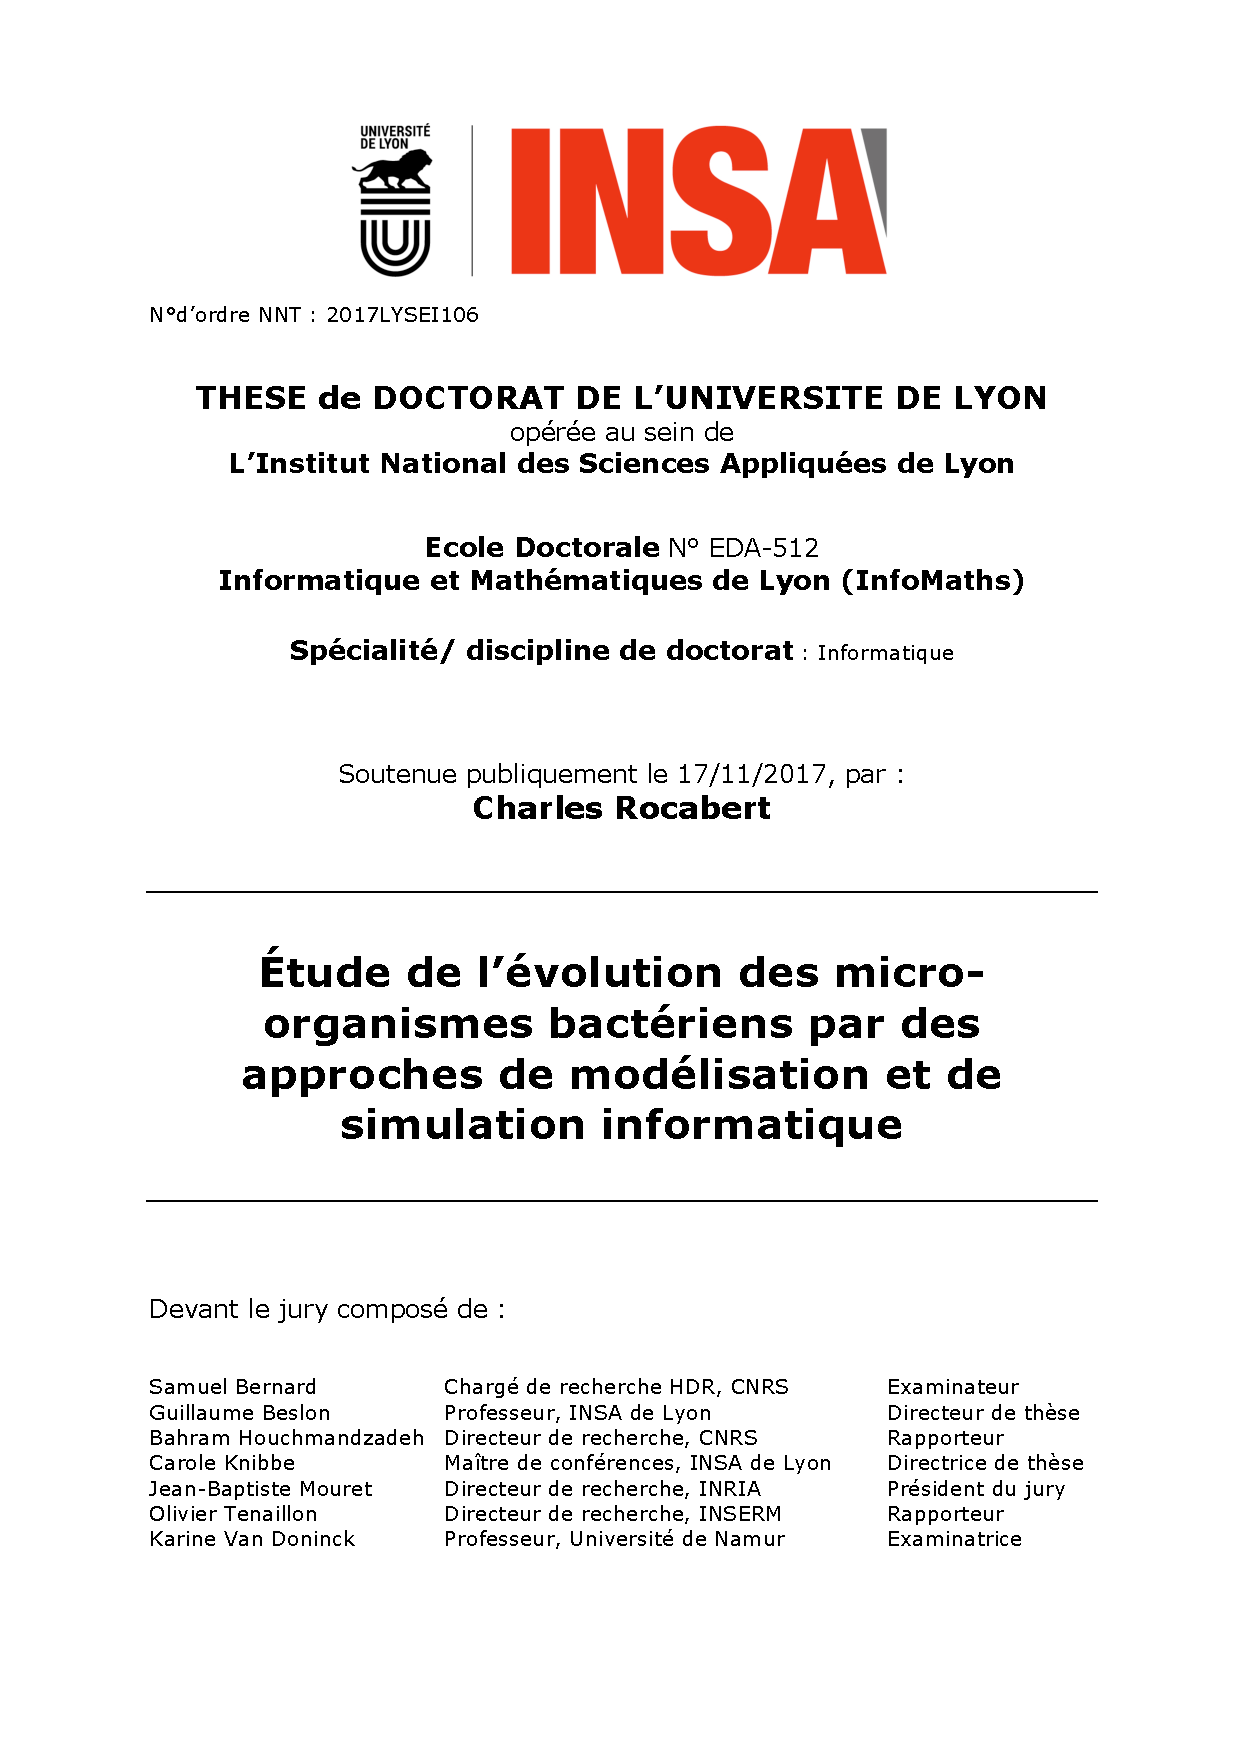
\includepdf[pages={1-}]{misc/header.pdf}

%%%%%%%%%%%%%%%%%%%%%%%%% HEADER PAGES %


\chapternonum{Remerciements}

Il y a neuf ans, je reprenais mes \'etudes \`a Lyon avec l'intention de faire de la recherche en biologie \'evolutive. Le monde universitaire et acad\'emique m'\'etait alors compl\`etement \'etranger. Aujourd'hui encore, chaque nouveau pas dans cet univers est une d\'ecouverte. Ce sont toutes les rencontres, scientifiques et humaines, qui ont fait de ces neuf ann\'ees les plus passionnantes et les plus riches de ma vie.
Je prends donc le temps ici d'\'evoquer les personnes qui ont compt\'e pour moi, sur une p\'eriode plus large que mes seules ann\'ees de th\`ese.

Tout d'abord, je remercie chaleureusement Jean-Baptiste Mouret et Karine Van Doninck d'avoir accept\'e de participer \`a mon jury de th\`ese, ainsi que Bahram Houchmandzadeh et Olivier Tenaillon pour leur relecture attentionn\'ee de ce manuscrit et leur retour positif.

Alors que j'\'etais en qu\^ete d'un stage de master 1, j'envoyai un mail laconique (``\textit{Je suis tr\`es int\'eress\'e par les travaux de votre \'equipe (COMBINING). Serait-il possible de vous rencontrer afin de discuter d'un \'eventuel stage ?}'') \`a un certain G\_\_ll\_\_\_ (barbu \`a l'\'epoque) qui m'invita imm\'ediatement \`a en discuter autour d'un caf\'e. Lorsque je lui pr\'esentai mon projet : \'etudier l'\'evolution de la stochasticit\'e d'expression des g\`enes avec {\aevol}, G\_\_ll\_\_\_  accepta sans h\'esitation (c'\'etait avant qu'il ne d\'ecouvre que je vouais un culte \`a K\_p\_\_\_).
Cela fait maintenant six ans que je tra\^ine dans les couloirs de Beagle, cela m'a laiss\'e le temps de comprendre pourquoi cette \'equipe est simplement la plus humaine et la plus soud\'ee que je connaisse. \`A l'\'evidence, c'est gr\^ace \`a toi Guillaume. Ton respect pour les go\^uts et les int\'er\^ets de chacun$\cdot$e, le fait que tu privil\'egies toujours le bien-\^etre des membres de l'\'equipe, sont la source de l'ambiance chaleureuse et unique qui r\`egne \`a Beagle. En quatre ann\'ees de th\`ese, j'ai appr\'eci\'e la disponibilit\'e et l'ouverture d'esprit dont tu fais preuve, malgr\'e un emploi du temps charg\'e. Tu m'as toujours fait confiance et laiss\'e libre de mes choix, tout en \'etant l\`a pour m'\'eclairer, me motiver et surtout, me faire prendre du recul. Tu t'en doutes certainement, ton approche et ta philosophie de la mod\'elisation ont eu une influence immense sur moi.

Comment remercier Guillaume sans remercier Carole, leur compl\'ementarit\'e est \'evidente. Carole, cette th\`ese n'aurait jamais aboutie sans ta contribution d\'ecisive. Tu as la capacit\'e de t'investir pleinement dans un travail de recherche, en ne laissant rien au hasard, et tu m'as transmis la pratique rigoureuse et objective de la science. Mais ce portrait serait bien r\'educteur, car tu t'es toujours souci\'ee de ma situation, et tu as toujours \'et\'e l\`a pour me soutenir et me conseiller.

En d\'ebut de th\`ese, alors que les lign\'ees Beagle et Dracula s'\'etaient un peu plus m\^el\'ees, Carole a demand\'e \`a Samuel de relire un obscur manuscrit rempli d'\'equations. Avec Sam, nous avons construit un vrai travail collaboratif, au point que je ne puisse dire de qui proviennent certaines id\'ees de notre mod\`ele. Sam, je n'oublierai jamais la confiance sereine que tu as eu en notre projet d\`es le d\'ebut -- ainsi que notre tentative d'entra\^inement au semi-marathon. J'esp\`ere que nous continuerons \`a travailler ensemble.

Carole, Guillaume et Samuel, je revendiquerai toujours votre h\'eritage. Pour tout cela, et plus encore, merci.

Ah, l'\'equipe Beagle, et son esprit d'ind\'ependance -- voire parfois de r\'esistance -- qui y r\`egne et que j'affectionne tant. Mettons \`a part les blagues douteuses de Huge Belly, qui en a traumatis\'e plus d'un$\cdot$e. Je pense au th\'esard$\cdot$e$\cdot$s bien-s\^ur : Priscilla, Vincent, Ilya, Sergio, Alexandre, Audrey, Marie, Alvaro, Jules, Marine, Yoram, avec qui j'ai pass\'e tant de bons moments. J'ai tout de m\^eme une pens\'ee particuli\`ere pour Jonathan et Vincent, avec qui nous avons partag\'e nombre de grenades lacrimog\`enes.
Hugues, qui a toujours \'et\'e l\`a pour m'\'ecouter et me conseiller, a \'et\'e l'un des organisateurs de l'\'ecole la plus passionnante \`a laquelle j'ai assist\'e\footnote{http://ecoleporquerolles.inria.fr/index.html}. Ton humour me manquera, Hugues ; que tu le veuilles ou non, tu es un des piliers de l'\'equipe Beagle. Merci \`a David -- qui m'a tant appris en informatique et en d\'eveloppement logiciel --, \'Eric, Christophe, H\'edi, Maurizio, Jaap, Ga\"elle et Nicolas, qui a eu le malheur de m'avoir comme enseignant. Je remercie aussi Caroline, qui a d\^u r\'eparer bien des bourdes administratives de ma part.

Dracula n'est pas en reste. Je pense notamment \`a Fabien, qui m'a souvent \'ecout\'e, aid\'e et encourag\'e. Je remercie \'egalement Olivier, qui conna\^it mon int\'er\^et pour le r\^ole du hasard dans le fonctionnement cellulaire, et qui m'a accueilli deux fois en stage.

Beagle, Dracula, vous me manquerez.

Le monde scientifique est petit, il y a un peu du LIRIS dans Beagle, et un peu du LEHNA dans le LIRIS. \`A ce croisement o\`u la bi\`ere bordelaise coule, naquit MoRIS. J\'er\^ome Gippet, mon ami de fac de toujours, et Serge Fenet, forgeron \`a ses heures perdues (ou bouilleur de cru ?), je vous dois cette belle aventure.
Un jour, J\'er\^ome m'a parl\'e d'un mod\`ele de propagation d'esp\`ece invasive qu'il avait en t\^ete. Quelques semaines plus tard \'etait n\'e MoRIS. D'un simple jouet, ce mod\`ele est devenu le fruit d'un v\'eritable travail collaboratif, avec financement, conf\'erences et publications \`a l'appui. J\'er\^ome, Serge, je n'oublierai jamais nos s\'eances de travail au milieu des Alpes et notre petit voyage \`a Bordeaux. MoRIS n'est qu'au d\'ebut d'une longue vie. Je remercie \'egalement Benjamin Galliot, pour son expertise en interface graphique, ainsi que Jean-Paul L\'ena, du LEHNA (ce n'est certainement pas un hasard) et Bernard Kauffman (du LEHNA aussi), pour nos discussions autour de votre inf\^ame caf\'e.

Un peu plus proche des Alpes, je me tourne maintenant vers le monde des bo\^ites de Petri et des micro-pipettes, pour remercier chaleureusement Dominique Schneider, Jessika Consuegra, et Otmane Lamrabet, ainsi que tous les membres de l'\'equipe grenobloise pour les vins-fromages du vendredi midi. Je remercie \'egalement tous les membres du projet EvoEvo, que j'ai eu la chance de c\^otoyer tout au long de cette th\`ese.

\`A propos de rencontres, beaucoup de choses se sont tram\'ees dans la r\'esidence \'etudiante Puvis de Chavannes. Je pense tout particuli\`erement \`a mon ami, Pierre Charrier, avec qui j'ai eu des discussions scientifiques passionn\'ees et partag\'e tant de lectures. Nous avons d\'ecouvert l'informatique ensemble, sur notre temps libre, alors que nous \'etudiions la biologie. Cet apprentissage autodidacte a \'et\'e d\'eterminant pour nous deux. Entre autres, Pierre avait dans sa chambre de 9 m\textsuperscript{2} une antenne wifi DIY en bo\^ite de conserve, une imposante collection d'insectes morts, et un \'equipement de culture hydroponique dans un placard -- pour des tomates.
Je pense aussi \`a mon autre ami d'infortune \'etudiante, Wam Human. Nous avons beaucoup de souvenirs en commun, entre randonn\'ees, s\'eances de grimpe, joggings \`a 6 heures du matin en d\'ecembre, ainsi que toutes nos soir\'ees \`a partager l'unique cuisine de notre \'etage avec Arnaud, Jacquou, Pierre et tant d'autres ; tout cela sous le regard bienveillant de Jean-Luc, le gardien de nuit de la r\'esidence.

Que serais-je devenu politiquement si Ivo Vassilev et Stan Chabert n'avaient pas \'et\'e l\`a ? Votre esprit militant a influ\'e sur toutes nos activit\'es, que ce soit en manif, en amphi, ou en soir\'ee. Je n'oublierai jamais les AGs de lutte \`a Lyon 1, les interventions de Stan, et la fameuse r\'eunion du POI. C'est aussi gr\^ace \`a vous deux -- et \`a vos colocs respectives -- que nous avons pu nous r\'eunir si souvent pendant les ann\'ees de licence.
Merci aussi \`a Perrine, pour les vir\'ees \`a Limas, ainsi qu'\`a Maxence, Magali, Julie, Cl\'ement, M\'elissa et tous les autres pour les bons souvenirs et les soir\'ees au petit parc.

Avant de me tourner vers ma famille, il y a trois autres personnes que j'aimerais citer. Annabelle, m\^eme si nous nous sommes perdus de vue depuis, c'est toi qui m'a fait d\'ecouvrir le travail de Jean-Jacques Kupiec, et qui a suscit\'e ma passion pour ce sujet en biologie. C'est aussi sous ton impulsion que nous avons fait notre premier stage ensemble, dans l'\'equipe d'Olivier Gandrillon. Je te remercie vraiment pour cela. Je pense aussi \`a Vincent Lacroix, qui repr\'esente pour moi ce que devrait \^etre l'enseignement universitaire : un travail d'\'emancipation collective, o\`u tout le monde est tir\'e vers le haut. Une derni\`ere personne que je veux remercier est Isabelle Illouz, qui s'est battue chaque ann\'ee pour que je puisse renouveler ma bourse \'etudiante et sans qui je n'aurais jamais pu poursuivre mes \'etudes.

Un grand merci \`a Fran\c coise, la maman de Manu\`ela, pour avoir toujours \'et\'e l\`a pour nous \'epauler, et nous avoir permis de respirer l'air frais des monts d'Ard\`eche toutes ces ann\'ees. Merci aussi \`a Alain pour les belles \'echapp\'ees dans les-dits monts, gr\^ace \`a son quad.

Je me tourne maintenant vers mes deux soeurs, Jeanne et Louise. Je vous dois la reprise de mes \'etudes. Vous m'avez r\'ev\'el\'e l'\'emancipation qu'apportent les \'etudes universitaires. L'\'el\'ement d\'eclencheur f\^ut un voyage au Royaume-Uni, mais votre influence oeuvrait depuis longtemps d\'ej\`a. Je ne vous remercierai jamais assez pour cela.

Maman et Papa, merci de m'avoir toujours laiss\'e libre de mes choix, et de m'avoir toujours soutenu, quelque f\^ut la direction que je pris. Papa, avec tes piles de Science \& Vie, et Maman avec ton intense activit\'e syndicale, vous m'avez appris \`a avoir un esprit critique. Je sais que vous \^etes fiers de moi pour cette th\`ese, mais au bout du compte, tout cela est de votre fait.

Manu\`ela, mon niabs, nous nous sommes rencontr\'es dans une r\'esidence \'etudiante, et depuis nous partageons tout. Je ne peux imaginer la vie sans toi. Durant ces longues ann\'ees de th\`ese, tu as \'et\'e mon \'echappatoire, la plupart de mes souvenirs vont vers toi. Tu m'as insuffl\'e ton courage pour traverser les \'epreuves, et tu m'as toujours tir\'e vers le haut. Ce manuscrit m\^eme porte ton empreinte, car il n'y a pas une figure, ou une mise en page qui ne viennent un peu de toi. Nous avons pleins de projets ensemble ; \`a tes c\^ot\'es, je n'aurai jamais peur d'avancer.

\begin{figurehere}
\centering
\includegraphics[width=1\textwidth]{tableau.pdf}
\caption*{\small{\textit{Par Manu\`ela, octobre 2017}}}
\end{figurehere}




\clearemptydoublepage


\chapternonum{R\'{e}sum\'{e}}

\section*{(en fran\c cais)}

Variation et s\'{e}lection sont au coeur de l'\'{e}volution Darwinienne. Cependant, ces deux m\'{e}canismes d\'{e}pendent de processus eux-m\^{e}me fa\c conn\'{e}s par l'\'{e}volution. Chez les micro-organismes, qui font face \`a des environnements souvent variables, ces propri\'{e}t\'{e}s adaptatives sont particuli\`erement bien exploit\'{e}es, comme le d\'{e}montrent de nombreuses exp\'{e}riences en laboratoire. Chez ses organismes, l'\'{e}volution semble donc avoir optimis\'{e} sa propre capacit\'{e} \`a \'{e}voluer, un processus que nous nommons \'{e}volution de l'\'{e}volution (EvoEvo).
La notion d'\'{e}volution de l'\'{e}volution englobe de nombreux concepts th\'{e}oriques, tels que la variabilit\'{e}, l'\'{e}volvabilit\'{e}, la robustesse ou encore la capacit\'{e} de l'\'{e}volution \`a innover (open-endedness). Ces propri\'{e}t\'{e}s \'{e}volutives des micro-organismes, et plus g\'{e}n\'{e}ralement de tous les organismes vivants, sont soup\c conn\'{e}es d'agir \`a tous les niveaux d'organisation biologique, en interaction ou en conflit, avec des cons\'{e}quences souvent complexes et contre-intuitives. Ainsi, comprendre l'\'{e}volution de l'\'{e}volution implique l'\'{e}tude de la trajectoire \'{e}volutive de micro-organismes -- r\'{e}els ou virtuels -- et ce \`a diff\'{e}rents niveaux d'organisation (g\'{e}nome, interactome, population, ...).

L'objectif de ce travail de th\`ese a \'{e}t\'{e} de d\'{e}velopper et d'\'{e}tudier des mod\`eles math\'{e}matiques et num\'{e}riques afin de lever le voile sur certains aspects de l'\'{e}volution de l'\'{e}volution. Ce travail multidisciplinaire, car impliquant des collaborations avec des biologistes exp\'{e}rimentateur$\cdot$rice$\cdot$s, des bio-informaticien$\cdot$ne$\cdot$s et des math\'{e}maticien$\cdot$ne$\cdot$s, s'est divis\'{e} en deux parties distinctes, mais compl\'{e}mentaires par leurs approches : \textbf{(i)} l'extension d'un mod\`ele historique en g\'{e}n\'{e}tique des populations -- le mod\`ele g\'{e}om\'{e}trique de Fisher -- afin d'\'{e}tudier l'\'{e}volution du bruit ph\'{e}notypique en s\'{e}lection directionnelle, et \textbf{(ii)} le d\'{e}veloppement d'un mod\`ele d'\'{e}volution \textit{in silico} multi-\'{e}chelles permettant une \'{e}tude plus approfondie de l'\'{e}volution de l'\'{e}volution.
Dans un premier temps, gr\^{a}ce \`a une version \'{e}tendue du mod\`ele de Fisher, nous avons montr\'{e} qu'un bruit corr\'{e}l\'{e} sur diff\'{e}rents caract\`eres ph\'{e}notypiques \'{e}volue sous s\'{e}lection directionnelle vers une forme bien particuli\`ere permettant de compenser en grande partie le co\^{u}t de la ``complexit\'{e} ph\'{e}notypique'', qui limite habituellement et fortement les chances de fixer des mutations favorables lorsque le nombre de caract\`eres sous s\'{e}lection est grand. Ces r\'{e}sultats prometteurs d\'{e}montrent l'importance et l'avantage s\'{e}lectif du bruit ph\'{e}notypique en s\'{e}lection directionnelle, et devrait susciter de nouveaux travaux de recherche, en collaboration avec des biologistes exp\'{e}rimentateur$\cdot$rice$\cdot$s.
Dans un deuxi\`eme temps, gr\^{a}ce au d\'{e}veloppement d'un mod\`ele d'\'{e}volution exp\'{e}rimentale \textit{in silico} multi-\'{e}chelles, nous avons pu reproduire virtuellement des approches exp\'{e}rimentales \textit{in vivo} -- notamment l'exp\'{e}rience d'\'{e}volution \`a long terme (LTEE) -- et ainsi contribu\'{e} \`a comprendre les ph\'{e}nom\`enes de construction de niche et d'\'{e}mergence d'un cross-feeding stable, pr\'{e}misses \`a la diversification et \`a la sp\'{e}ciation bact\'{e}rienne.
Ce mod\`ele d'\'{e}volution \textit{in silico} nous a \'{e}galement permis de nous interroger sur l'\'{e}mergence et l'\'{e}volution de la r\'{e}gulation g\'{e}n\'{e}tique, comme solution au maintien de l'\'{e}conomie \'{e}nerg\'{e}tique de la cellule. Nos r\'{e}sultats, encore pr\'{e}liminaires, confirment l'id\'{e}e que le r\^{o}le de la r\'{e}gulation g\'{e}n\'{e}tique n'est pas d'ajuster le m\'{e}tabolisme aux conditions environnementales, mais plut\^ot d'assurer l'\'{e}conomie \'{e}nerg\'{e}tique interne et la survie de la cellule, ind\'{e}pendamment des variations environnementales. Ces premiers r\'{e}sultats sugg\`erent \'{e}galement que la structuration des g\'{e}nomes bact\'{e}riens est fortement influenc\'{e}e par les contraintes \'{e}nerg\'{e}tiques internes.

Cette th\`ese a \'{e}t\'{e} financ\'{e}e par le projet europ\'{e}en EvoEvo (FP7-ICT-610427), gr\^{a}ce \`a la commission europ\'{e}enne.

\section*{(in english)}

Variation and selection are the two core processes of Darwinian Evolution. Yet, both are directly regulated by many processes that are themselves products of evolution. Microorganisms efficiently exploit this ability to dynamically adapt to new conditions. Thus, evolution seems to have optimized its own ability to evolve, as a primary means to react to environmental changes. We call this process evolution of evolution (EvoEvo). EvoEvo covers several aspects of evolution, encompassing major concepts such variability, evolvability, robustness, and open-endedness. Those phenomena are known to affect all levels of organization in bacterial populations. Indeed, understanding EvoEvo requires to study organisms experiencing evolution, and to decipher the evolutive interactions between all the components of the biological system of interest (genomes, biochemical networks, populations, ...).
The objective of this thesis was to develop and exploit mathematical and numerical models to tackle different aspects of EvoEvo, in order to produce new knowledge on this topic, in collaboration with partners from diverse fields, including experimental biology, bioinformatics, mathematics and also theoretical and applied informatics. To this aim, we followed two complementary approaches: \textbf{(i)} a population genetics approach to study the evolution of phenotypic noise in directional selection, by extending Fisher's geometric model of adaptation, and \textbf{(ii)} a digital genetics approach to study multi-level evolution. This work was funded by the EvoEvo project, under the European Commission (FP7-ICT-610427).


\clearemptydoublepage


\chapternonum{Liste des publications personnelles}

\section*{Articles parus}

\begin{itemize}
\item \textbf{Rocabert, C.}, Knibbe, C., Consuegra, J., Schneider, D., \& Beslon, G. (2017). Beware batch culture: Seasonality and niche construction predicted to favor bacterial adaptive diversification. \textit{PLoS Computational Biology}, 13(3), e1005459.
\item \textbf{Rocabert, C.}, Knibbe, C., \& Beslon, G. (2015, July). Towards a Integrated Evolutionary Model to Study Evolution of Evolution. In Proceedings of \textit{the First EvoEvo Workshop (Satellite workshop of ECAL 2015)} (York, UK).
\end{itemize}

\section*{Articles soumis ou en pr\'eparation}
\begin{itemize}
\item \textbf{Rocabert, C.}, Bernard, S., Beslon, G., \& Knibbe, C. (2017). Phenotypic Noise and the Cost of Complexity. \textit{Evolution}, under review.
\item Gippet M.W., J., \textbf{Rocabert, C.}, Fenet, S., \& Kaufmann, B. MoRIS: Model of Routes of Invasive Spread. Human-mediated dispersal, road network and invasion parameters. In preparation.
\end{itemize}

\section*{Résumés des conférences}
\begin{itemize}
\item \textbf{Rocabert, C.}, Knibbe C., Consuegra J., Schneider D., \& Beslon G. (2017, September) Environmental seasonality drives digital populations towards stable cross-feeding. In Proceedings of \textit{ECAL 2017 conference. 14\textsuperscript{th} European Conference on Artificial Life} (Lyon, France). Communication orale
\item \textbf{Rocabert, C.}, Knibbe, C., Consuegra, J., Schneider, D., \& Beslon, G. (2016, September). In Silico Experimental Evolution Highlights the Influence of Environmental Seasonality on Bacterial Diversification. In Proceedings of \textit{the Second EvoEvo Workshop. Satellite workshop of CCS2016} (Amsterdam, Netherlands). Communication orale
\item Gippet, J., Fenet, S., Dumet, A., Kaufmann, B. \& \textbf{Rocabert, C.} (2016, August) MoRIS: Model of Routes of Invasive Spread. Human-mediated dispersal, road network and invasion parameters. In Proceedings of \textit{IENE 2016 conference. 5\textsuperscript{th} International Conference on Ecology and Transportation: Integrating Transport Infrastructures with Living Landscapes} (Lyon, France). Communication orale par J. Gippet.
\item \textbf{Rocabert, C.}, Knibbe, C., Consuegra, J., Schneider, D. \& Beslon, G. (2016, April). In Silico Experimental Evolution Highlights the Influence of Environmental Seasonality on Bacterial Diversification. In \textit{EvoAct: Evolution in action with living and artificial organisms conference} (Autrans, France). Communication orale
\item \textbf{Rocabert, C.}, Knibbe C., Consuegra J., Schneider D., \& Beslon G. (2016, March) Environmental Driving of Bacterial Diversification in In Silico Experimental Evolution. In \textit{Evolutionary systems biology: from model organisms to human disease workshop}, (Cambridge, UK). Poster
\item Gippet, J., \textbf{Rocabert, C.}, Fenet, S., Dumet, A., \& Kaufmann, B. (2015, July). Modeling and evaluating human-mediated dispersal mechanisms at landscape scale: a study of road network and invasion parameters for Lasius neglectus ants invasive species. In Proceedings of \textit{World Conference on Natural Resource Modeling} (Bordeaux, France). Communication orale par J. Gippet.
\end{itemize}

\clearemptydoublepage

%%%%%%%%%%%%%%%%%%%%%%%%% TABLES OF CONTENT %

\tableofcontents
\markboth{Table of contents}{Table of contents}

\clearemptydoublepage

\listoffigures
\markboth{List of figures}{List of figures}

\clearemptydoublepage

\listoftables
\markboth{List of tables}{List of tables}

\clearemptydoublepage

%%%%%%%%%%%%%%%%%%%%%%%%% FOREWORD %


%%%%%%%%%%%%%%%
%%%      CHAPTER      %%%
%%%%%%%%%%%%%%%

\chapternonum{Foreword}
\label{ch:general_introduction:foreword}
\addcontentsline{toc}{chapter}{Foreword}

I precisely remember the first book of theoretical biology I read. At this time, I was an aircraft mechanic, apparently far from the academic world. With \textit{Chance and Necessity}, Jacques Monod made a remarkable demonstration of the central dogma of molecular biology, introduced 12 years ago by Francis Crick \citep{crick-1958}. As a novice, I have been impressed by the clarity and the rigor of this philosophical essay, stamped with a certain arrogance to have explained everything about life on Earth.

\begin{quote}
L'ultima ratio de toutes les structures t\'{e}l\'{e}onomiques des \^{e}tres vivants est donc enferm\'{e}e dans les s\'{e}quences de radicaux des fibres polypeptidiques, ``embryons'' de ces d\'{e}mons de Maxwell biologiques que sont les prot\'{e}ines globulaires. En un sens, tr\`es r\'{e}el, c'est \`a ce niveau d'organisation chimique que g\^{i}t, s'il y en a un, le secret de la vie. Et saurait-on non seulement d\'{e}crire ces s\'{e}quences, mais \'{e}noncer la loi d'assemblage \`a laquelle elles ob\'{e}issent, on pourrait dire que le secret de la vie est perc\'{e}, l'ultima ratio d\'{e}couverte \citep{monod-1970}.
\end{quote}

This book sowed the seeds of my fascination for evolutionary biology.
In the following year, I went back to school with this kind of convictions: living organisms own a ``genetic program'', encoding for their phenotype.
This program is regularly altered by purely random mutations, thereby providing the fuel for evolution. I found comfortable consistency with this dogma in the first lessons I followed at university. The apotheosis has probably been reached on reading \textit{The Selfish Gene} by Richard Dawkins \citep{dawkins-1976}.

During my first year of college, I met astonishing people\footnote{See the acknowledgments.} that pushed me to take a more measured look at theoretical biology. In particular, I had the opportunity to read the work of Jean-Jacques Kupiec \citep{kupiec-2000,kupiec-2008}, a fervent partisan of nominalism in science, that definitively influenced my scientific itinerary. While J-J. Kupiec's narrative is tinged with a touch of bitterness, his epistemology has the merit to promote thought and criticism. I will always remember the little joke I heard at the time: ``\textit{People believing that stochastic gene expression is important are often to the left, people believing that a genetic program exists are often to the right}''\footnote{A classical debate between essentialist and nominalist views in sum.}. 

Armed with this very small, but necessary epistemological knowledge, I finally read \textit{On the Origin of Species} by Charles Darwin. I was not surprised to discover that his reasoning was almost at the opposite from Jacques Monod's ones. While the latter stated that the three properties distinguishing living organisms from the rest of the universe were teleonomy, autonomous morphogenesis and reproductive invariance, Charles Darwin original theory defined individual differences and natural selection as the main properties of life.

\begin{quote}
No one supposes that all the individuals of the same species are cast in the very same mould. These individual differences are highly important for us, as they afford materials for natural selection to accumulate, in the same manner as man can accumulate in any given direction individual differences in his domesticated productions \citep{darwin-1859}.
\end{quote}

Indeed, a form of essentialism flowed back in biology in the 1960's, mainly following Erwin Schr\"odinger's book \textit{What is Life?} \citep{schrodinger-1944}, and the discover of DNA structure \citep{avery-et-al-1944,watson-et-al-1953}. According to E. Schr\"odinger, most physical properties on a large scale (\textit{e.g.} diffusion process or kinetic theory of gases) emerge from chaos at a low scale: this property is known as the principle of order-from-disorder. On the contrary, living matter ``\textit{is likely to involve `other laws of physics' hitherto unknown, which however, once they have been revealed, will form just as integral a part of science as the former}'' \citep{schrodinger-1944}. E. Schr\"odinger was believing in a principle of order-from-order, the living matter escaping from thermodynamics laws. This point of view, while probably never accepted as is by convinced darwinists\footnote{In \textit{Chance and Necessity}, J. Monod largely argued against the principle of order-from-order in life. However, all the paradox of his interpretation of life resurged when he used the term ``Maxwell's demons'' to design enzymes.}, still influences nowadays scientific works.

\begin{quote}
Pour la biologie mol\'{e}culaire, l'organisme est donc toujours une machine d\'{e}terministe, mais la vieille horloge de Descartes a \'{e}t\'{e} remplac\'{e}e par un ordinateur \citep{kupiec-2008}.
\end{quote}

As a consequence, a paradoxical representation of life pervaded theoretical biology for decades: while a small ``Copernican revolution'' was accomplished in evolutionary biology with C. Darwin, a strong essentialism was hidden in the wood, particularly in molecular biology.

One example is the strong belief that genes are the fundamental units of natural selection. Initially, genes have been defined as inheritable units predetermining\footnote{One could ask why a causation was introduced, while just a correlation was observed.} phenotypic traits \citep{johannsen-1911} (W. Johannsen also introduced the notions of genotype and phenotype). As discussed right above, the discover of DNA and the mechanisms of gene expression reinforced this view and led to a ``genocentric'' view of evolution, with a clear separation between the genotype, undergoing mutations and inherited, and the phenotype \citep{rivoire-and-leibler-2014}. This net separation is often criticized as a resurgence of an Aristotelian interpretation of life\footnote{The model (the essence) of an organism is encoded in its genotype, out of the scope of natural selection (in the world of ideas), its phenotype being an imperfect instantiation of the model (in the sensible world).}, against the evident nominalism of C. Darwin. \textit{The selfish gene} by \cite{dawkins-1976} is often cited as a culmination of genetic reductionism in biology.

Another consequence of essentialism in biology is the belief that mutations purely occur at random. As stated by \cite{monod-1970}, the purpose---or teleonomy---of any living organism is to transmit its intact genotype---by reproductive invariance---to its offspring. Of course, as explained by J. Monod himself, teleonomy is not teleology: the apparent finalism of life is a consequence of natural selection. But the damage is done: in the face of teleonomy and reproductive invariance, the way mutations occur is necessarily out of the scope of selection. For decades, any statement that organisms could partly control the way mutations occur (\textit{e.g.}, the evolution of mutation rates, globally or locally on the genome), was accused of finalism---which is indeed quite paradoxical. In the last decades, this dogmatic view has been undermined by experimental an theoretical highlights, leading to the idea that evolution could shape its own fate. This phenomenon is usually known as the evolution of evolvability.

A last example I would give is the classical interpretation of organismal development as a genetic program, deterministically expressing the phenotype from the genotype:
``\textit{chaque \oe uf contient donc, dans les chromosomes re\c cus de ses parents, tout son propre avenir, les \'etapes de son d\'eveloppement, la forme et les propri\'et\'es de l'\^etre qui en \'emergera. L'organisme devient ainsi la r\'ealisation d'un programme prescrit par l'h\'er\'edit\'e}'' \citep{jacob-1970}\footnote{These words could remind the preformationist views developed during the XVII\textsuperscript{th} century.}.
An essential role is attributed to the concept of protein stereospecificity, conferring to the cell the ability to run deterministic and logical tasks based on signaling and regulation pathways. As stated by \cite{kupiec-2008}: ``\textit{bien que cela soul\`eve de nombreux probl\`emes, ce programme g\'{e}n\'{e}tique a \'{e}t\'{e} con\c cu par analogie avec un programme informatique}''. However, biochemical reactions do not escape thermodynamics laws, and the low number of molecules involved in many biological processes implies that ``\textit{chance is at the heart of the cell}'' \citep{gandrillon-et-al-2012}. Nowadays, the stochastic nature of cellular functioning is widely documented and accepted, but its consequences on the evolution of biological organisms are still largely unknown.

Of course, there is no sense to criticize \textit{a posteriori} the work of an entire scientific community, without considering the extraordinary progresses of biology during the XX\textsuperscript{th} century.
This is why my thesis work will be mostly based on the rationale that the tools and models of theoretical evolutionary biology proven to be efficient can be revisited, extended or modified to ask new scientific questions.

The starting point of my thesis work is the process of evolution of evolution, or EvoEvo, as coined by \cite{hindre-et-al-2012}, that encompasses the evolution of variability, evolvability, robustness and open-endeness.

There is no scientific theory without modeling \citep{servedio-et-al-2014}. I explored two different---but not opposite---modeling approaches to study EvoEvo: mathematical modeling and multi-scale individual-based simulations. On this particular point, I have been strongly influenced all along my stay in the INRIA-Beagle team by the complementary approach of Carole Knibbe and Guillaume Beslon, well-resumed by the quadruplet ``\textit{Create, Play, Experiment, Discover}'', used as a slogan for the 14\textsuperscript{th} European Conference on Artificial Life.

As explained in chapter \ref{ch:general_introduction:introduction}, there is a deep sense to tackle EvoEvo by these two modeling sides. The first, and most obvious reason is that analytical demonstrations are needed to sit a theory and convince a scientific community. The second reason is more specific to EvoEvo: the evolution of an organism implies the interaction of many biological organization levels, with different temporalities and scales. To properly understand how evolution shapes such a complex system, we need to simulate it with a multi-scale model catching, at least partially, this complexity \citep{lavelle-et-al-2008}. As stated by S. L. Peck: ``\textit{The world is complex and we need all the tools that we can muster to understand it}'' \citep{peck-2004}.

This manuscript is structured as following: in a first chapter, I will introduce the concept of evolution of evolution, and the modeling approaches used to decipher some of its aspects. Then, in part \ref{part1}, I will present a mathematical modeling study on the evolution of phenotypic noise. This model extends Fisher's geometric model \citep{fisher-1930}. In part \ref{part2}, I will introduce {\EvoEvoSim}, a multi-scale model of \textit{in silico} experimental evolution \citep{hindre-et-al-2012} dedicated to the study of evolution of evolution (chapter \ref{ch:part2:methodology}). Two results obtained with this model will be presented, one on niche construction and the evolution of stable cross-feeding (chapter \ref{ch:part2:first_result}), another on the evolution of regulation when organisms undergo strong energy trade-offs (chapter \ref{ch:part2:second_result}).

Some of these results have been published, or submitted to scientific journals. Others come from documents produced in the course of the FP7 EvoEvo project I were involved in, or are preliminary. I will indicate it when it will be the case. This manuscript also contains appendices; I will refer to them in the main text when necessary.

\newpage

\begin{quote}
Some rain forests in the Amazon region occur on white-sand soils. In these locations, the physical environment consists of clean white sand, air, falling water, and sunlight. Embedded within this relatively simple physical context, we find one of the most complex ecosystems on earth, containing hundreds of thousands of species. These species do not represent hundreds of thousands of adaptations to the physical environment. Most of adaptations of these species are to the other living organisms. The forest creates its own environment. \citep{ray-1993}
\end{quote}

\begin{figure}[!h]
\centering
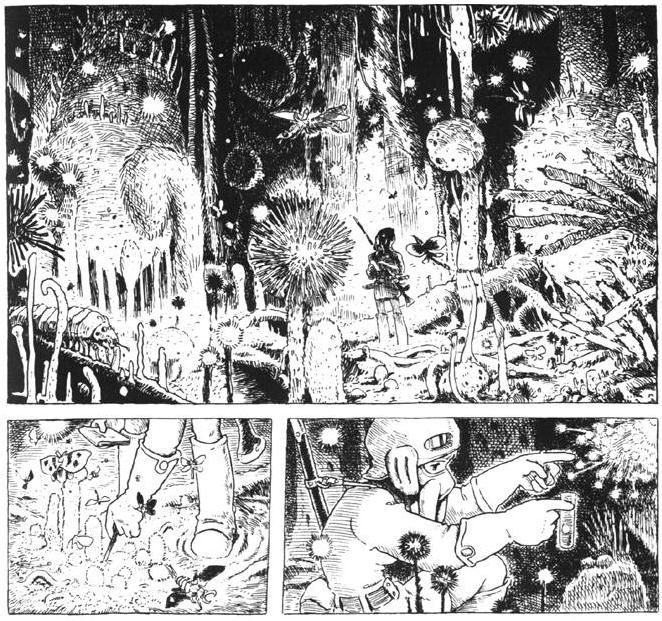
\includegraphics[width=0.8\textwidth]{nausicaa.jpeg}
\caption[An example of complex ecosystem.]{{\bf An example of complex ecosystem.} From \textit{Nausica\"a}, by Hayao Miyazaki.}
\label{fig:nausicaa}
\end{figure}



%%%%%%%%%%%%%%%%%%%%%%%%%% GENERAL INTRODUCTION %


%%%%%%%%%%%%%%%
%%%      CHAPTER      %%%
%%%%%%%%%%%%%%%

\chapter{Introduction}
\label{ch:general_introduction:introduction}

%%%%%%%%%%%%%%%%%%%%%%%%%%%%%%%%%%%%%%%%%
%%%%%%%%%%%%%%%%%%%%%%%%%%%%%%%%%%%%%%%%%

\section{The limits of the modern synthesis}
\label{sec:general_introduction:introduction:darwin_limits}

Variation and selection are at the core of evolution \citep{darwin-1859}. In theory, these two mechanisms are sufficient to engage a process of Darwinian evolution, where differences in reproduction and survival rates---summarized by the concept of \textbf{fitness}---lead to the ``survival of the fittest'' \citep{spencer-1864}. During the XX\textsuperscript{th} century, the modern synthesis has been developed to rise this mechanism as the central paradigm of biology, merging C. Darwin's and G. Mendel's theories \citep{huxley-1942} (Fig. \ref{fig:general_introduction:introduction:fig1}). Variation and selection are also exploited in other fields such as evolutionary optimization algorithms. However, while the modern synthesis mostly focused on molecular evolution, at the level of the \textbf{genotype} (by attributing a fitness to an allele segregating in the population for example), selection actually plays on the \textbf{phenotype} of an organism \citep{lande-1976}. Despite the attempt of quantitative genetics to link phenotypic variability with genetic mutations, the relationship between the genotype and the phenotype, known as the \textbf{genotype-to-phenotype map} \citep{alberch-1991}, is far from being understood, and classical models of evolution are unable to explain the most integrated properties of living organisms, \textit{e.g.}, phenotypic innovations or major transitions \citep{smith-szathmary-1997}. Three main reasons could be invoked to explain the apparent failure of modern synthesis to model the most complex evolutionary outcomes:

\begin{figure}[!h]
\centering
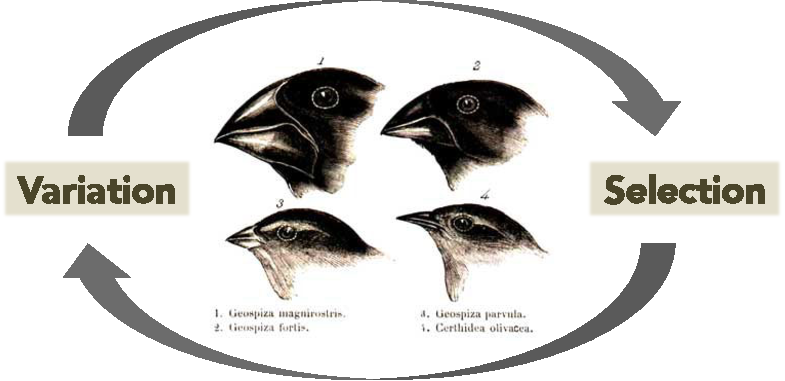
\includegraphics[width=0.6\textwidth]{generalintroduction_introduction_fig1.pdf}
\caption[Variation and selection at the heart of Darwinian evolution.]{{\bf Variation and selection at the heart of Darwinian evolution.} As symbolically represented by the Darwin finches, whose beaks are adapted to various sizes and shapes of seeds, variation and selection are at the heart of Darwinian evolution, a theoretical basis to the modern synthesis.}
\label{fig:general_introduction:introduction:fig1}
\end{figure}

\paragraph{$\bullet$ Biotic systems process information.}
In the early 1970's, Paulien Hogeweg and Ben Hesper coined the term ``bioinformatics'' to design the study of ``informatic processes in biotic systems'' \citep{hogeweg-hesper-1978,hogeweg-1978}. Even if the term has later been distorted to refer to biological data analysis, an important idea was released: according to P. Hogeweg, ``\textit{it seemed to us that one of the defining properties of life was information processing in its various forms, e.g., information accumulation during evolution, information transmission from DNA to intra and intercellular processes, and the interpretation of such information at multiple levels}'' \citep{hogeweg-2011}. Indeed, an essential property of living species seems to be their ability to accumulate information from past environments, on the long-term. By ``learning'' about past environmental features, species can ``react'' to new environments, by enhancing their \textbf{evolvability} (\textit{e.g.}, by increasing mutation rates, or favoring mutations in a specific region of their genome, ...), or their \textbf{robustness} (\textit{e.g.}, by evolving DNA repair mechanisms, or by buffering genetic variations through the regulation network, ...). During the last decades, this property of evolution received a lot of interest, and is often referred as \textbf{evolution of evolvability}\footnote{The concept of information accumulation and ``evolution learning'' is also a concern of the \textbf{extended evolutionary synthesis}, an attempt to extend the modern synthesis \citep{laland-et-al-2015,watson-szathmary-2016}.}.

\paragraph{$\bullet$ Evolution acts at multiple levels.}
In 2003, Paulien Hogeweg and Nabuto Takeuchi noticed that: ``\textit{although there has been much discussion on what is the appropriate level on which Darwinian selection operates, we now know that in many cases the interesting features arise through the occurrence of multiple levels of selection which act in concordance and/or in conflict}'' \citep{hogeweg-and-takeuchi-2003}. While the definition of ``level'' is the source of a classical debate in biology\footnote{See \cite{banzhaf-et-al-2016} for a discussion on the notion of ``biological level''.}, one would hardly disagree that life takes place on multiple physical and time scales. A living organism is composed of one or more cells, each containing a cytoplasm with numerous and complex structures, DNA, RNA, proteins and so on. Each organism interacts with its environment and with other organisms. Populations of organisms modify their environment, creating new selective pressures, and various species interact together, directly or indirectly. Life on earth thus scales from molecules to entire ecosystems, all of these structures interacting and evolving in concert. Here, a question rises about how to model such a complex system. Nobody pretends to be able to forecast the weather by only simulating a set of gas molecules under brownian motion. With such a low-scale modeling, important properties of weather, such as gravity and Coriolis forces, temperature gradients or day/night cycles will never emerge from the model. This is quite similar in evolutionary biology: a gene-centered model will not be able to produce the most integrated properties of evolution, simply because there is no support in the model for it \citep{banzhaf-et-al-2016}. To do so, \textbf{multi-level models} are needed.

\paragraph{$\bullet$ Interesting properties of evolution emerge with second-order selection.}
According to \cite{tenaillon-et-al-2001}, the Darwinian view of evolution needs a refinement to explain its ``complex dynamic aspects''. More than just a selection for better adaptation to a specific environment, \textbf{second-order selection}, or \textbf{indirect selection} \citep{kirschner-gerhart-1998,reisinger-miikkulainen-2006}, acts on the regulation of the processes of adaptation to any new environment \citep{pennisi-1998}. Some survival strategies could not evolve without second-order selection, such as evolution of mutation rates and mutators \citep{denamur-matic-2006}, or evolution of bet-hedging \citep{beaumont-et-al-2009} for example. Second-order selection is also responsible for the emergence of important processes discussed just above, such as information accumulation in biotic systems.

Finally, as shown in Figure \ref{fig:general_introduction:introduction:fig2}, long-term evolution and second-order selection led to the emergence of many mechanisms observed in living systems, at all the biological organization levels. These mechanisms directly control the variability of organisms, and are themselves under selection. Hence, we can expect that living organisms, more than being adapted to their environment, \textbf{are adapted to evolve}. \cite{hindre-et-al-2012} coined the term \textbf{evolution of evolution} (EvoEvo) to refer to this evolutionary process.

\begin{figure}[!h]
\centering
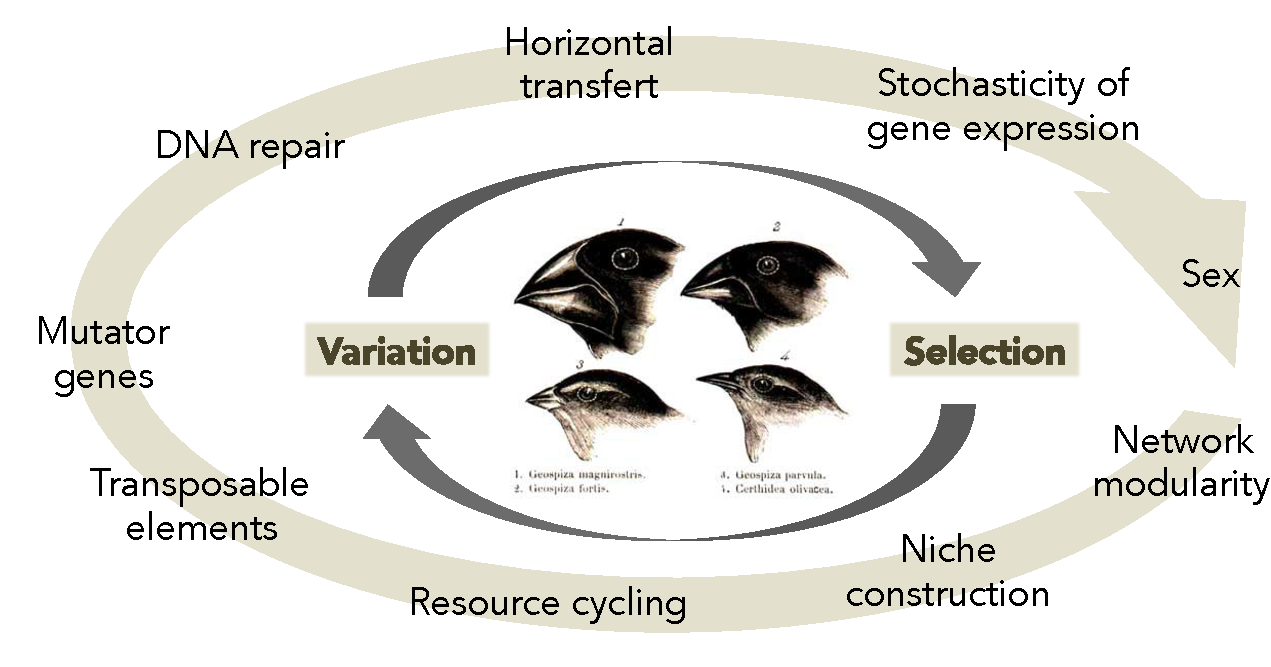
\includegraphics[width=1\textwidth]{generalintroduction_introduction_fig2.pdf}
\caption[Long-term evolution leads to evolution of evolution.]{{\bf Long-term evolution leads to evolution of evolution.} On the long-term, living organisms have evolved different mechanisms (DNA repair, horizontal transfer, sex, and so on) that control their own variability. However, these mechanisms are themselves under selection, implying that the basic mechanisms of evolution are therefore themselves evolving, a process called evolution of evolution, or EvoEvo.}
\label{fig:general_introduction:introduction:fig2}
\end{figure}

%%%%%%%%%%%%%%%%%%%%%%%%%%%%%%%%%%%%%%%%%%
%%%%%%%%%%%%%%%%%%%%%%%%%%%%%%%%%%%%%%%%%%

\section{What is evolution of evolution?}
\label{sec:general_introduction:introduction:what_is_evoevo}

By evolving, living organisms permanently adapt to rarely stable and sometimes unpredictable environments. Moreover, organisms constantly modify their environment, by interacting with it and by evolving, thus generating complex and challenging conditions. While higher eukaryotes have evolved complex sensori-motor systems to plastically adapt to environmental variations, micro-organisms (that represent more than an half of the biomass on earth) do not have such complex sensoring abilities. However, they are surprisingly efficient to adapt to their environment by simply ... evolving. Many experimental studies demonstrated that bacteria and viruses are able to adapt to new environments in only a few tens of generations \citep{rainey-travisano-1998,zhang-et-al-2011}. Hence, micro-organisms are excellent candidates to study evolution of evolution \citep{hindre-et-al-2012}.

EvoEvo encompasses the evolution of four essential evolutionary properties: \textbf{variability}, \textbf{evolvability}, \textbf{robustness}, and \textbf{open-endedness}. While the notions of evolvability and robustness pervaded theoretical evolutionary biology during the last decades, the concept of open-endedness is more familiar to computational scientists. However, it is strongly related to \textbf{phenotypic innovations} and \textbf{major transitions} \citep{smith-szathmary-1997}, two important concepts in evolutionary biology.

%%%%%%%%%%%%%%%%%%%%%%%%%%

\subsection{Variability}
Variability is the ability to generate new phenotypes. It is a necessary condition for any evolutionary process to take place. A lot of biological mechanisms have been identified that produce and/or control variability:
\begin{enumerate}
% GENETIC VARIABILITY
\item[\textbf{(1)}] \textbf{Genetic variability.}  For historical reasons, genetic variability has been widely studied during the XX\textsuperscript{th} century, and a variety of mutational events altering genomes have been identified (point mutations, small insertions and deletions, large rearrangements, horizontal transfers, gene amplifications, ...). Many mechanisms are known to modify the rate at which these mutation events occur in the genome, locally or globally, as reviewed in \cite{ryall-et-al-2012}. For example, when \textbf{contingency loci}---localized on small portions of the genome---are mutated, mutation rates are locally increased. Another example is \textbf{mutations in DNA repair or maintenance genes}, that can lead to hyper-mutator strains, which have constitutively elevated mutation rates. In some conditions, these strains can be positively selected and favor adaptation \citep{tenaillon-et-al-1999,denamur-matic-2006}. As a last example, \textbf{transient changes in the expression level of DNA repair and maintenance genes} allow for rapid mutation rates increase in case of environmental stress \citep{foster-2007};
% PHENOTYPIC PLASTICITY
\item[\textbf{(2)}] \textbf{Phenotypic plasticity.}
According to \cite{stearns-1989}, phenotypic plasticity refers to phenotypic variability in response to the environment. Micro-organisms own genetic regulation networks, able to sense their environment. Evolution can shape these regulation networks such that one genotype can produce many phenotypes as a function of an environmental signal (the reaction norm). When one genotype produces several discrete phenotypes depending on the environmental signal, we speak about \textbf{polyphenism}. When one genotype produces a single phenotype, whatever the environmental variations, we speak about \textbf{environmental canalization}, one source of evolutionary robustness \citep{waddington-1942};
% EPIGENETIC INHERITANCE
\item[\textbf{(3)}] \textbf{Transgenerational epigenetic inheritance.}
According to \cite{veening-et-al-2008}, epigenetic inheritance refers to any transmission of a cellular state from one generation to another without genome modification. A classical example of this mechanism is DNA methylation or acetylation \citep{avery-2006}.
For example, the agouti yellow mouse phenotype is due to the unmethylation of the retrotransposon gene \textit{Avy}, inserted upstream of \textit{agouti} gene. Agouti yellow mices have yellow coat and suffer obesity. It appeared that unmethylated sequences are transmissible from one generation to the other via the gametes, without modification of the genotype.
% PHENOTYPIC STOCHASTICITY
\item[\textbf{(4)}] \textbf{Phenotypic stochasticity.}
Finally, the stochastic fluctuations of the phenotype (or phenotypic noise) are an important source of variability \citep{symmons-and-raj-2016}. Phenotypic noise is mainly due to the inherent stochastic nature of biochemical reactions inner the cell, because of the low number of implicated molecules and thermodynamic fluctuations. An example is \textbf{stochastic gene expression} (SGE). SGE has an important role in genetic regulation and the emergence of interesting phenotypic properties such as stochastic switching \citep{acar-et-al-2008,tsuru-et-al-2011}. Stochastic fluctuations are of primary importance in some survival strategies, such as bet-hedging \citep{veening-et-al-2008}, as reviewed in details by \cite{dejong-et-al-2011}. The evolution of phenotypic noise will be studied in part \ref{part1} of this manuscript.
\end{enumerate}

All these mechanisms being themselves under selection, we can expect that variability---and thus evolution---can evolve.

%%%%%%%%%%%%%%%%%%%%%%%%%%

\subsection{Evolvability and robustness}
The question of the evolution of evolvability and its relationship with the evolution of robustness has received important contributions in the last years. However, the question is still open. While the term evolvability has been used in different ways \citep{wagner-2013}, it is usually defined as \textbf{the ability to increase the proportion of beneficial mutations}, while robustness is defined as \textbf{the ability to withstand mutations without losing fitness}. Both mechanisms has been shown to evolve, mainly in numerical simulations (see \textit{e.g.} \citealt{bedau-packard-2003,elena-sanjuan-2008,crombach-hogeweg-2008,beslon-et-al-2010a}). Demonstrating evolution of evolvability or robustness experimentally is much more difficult since it necessitates to perform experimental evolution experiments, which are long and costly (see \textit{e.g.} \citealt{elena-and-lenski-2003}).

At first sight, evolvability and robustness seem to be antagonistic. An evolvable organism should not be robust, and a robust organism should not be evolvable. However, the remarkable ability of Darwinian evolution to generate sophisticated emergent properties is demonstrated here. Indeed, evolvability has an important role in \textbf{innovation}: a biological system is evolvable if it can acquire novel functions through genetic change that increase fitness \citep{wagner-2005}. However, and counter-intuitively, robustness and \textbf{neutral mutations} also play a key role in the innovation process, because they allow to explore the phenotypic space while the fitness of the organism remains constant. By exploring the neutral landscape of an organism, neutral mutations promote future innovation.

This mechanism has nicely been represented by \cite{wagner-2008b} (Fig. \ref{fig:general_introduction:introduction:fig3}). Let's consider a network of all possible genotypes of an organism, each node being a genotype, linked to accessible other genotypes by single mutations. A fitness is attributed to each genotype. Some mutations are neutral, meaning that they link two genotypes with the same fitness, negative (if they decrease the fitness), or positive. A positive mutation can also be an innovation (the acquisition of a novel function with a beneficial fitness value, as discussed later in this introduction). For a robust organism, many mutations are neutral, such that evolution consists to travel in the neutral genotype network. Robust organisms can thus explore vast regions of the genotype network with no consequence on their fitness, and access new genotypes not accessible otherwise. As metaphorically stated by A. Wagner:
\begin{quote}
Perhaps the most compact way to express this problem is with an analogy from politics: evolving populations need to be both ``conservative'' and ``progressive'' at the same time \citep{wagner-2012}.
\end{quote}

\begin{figure}[!h]
\centering
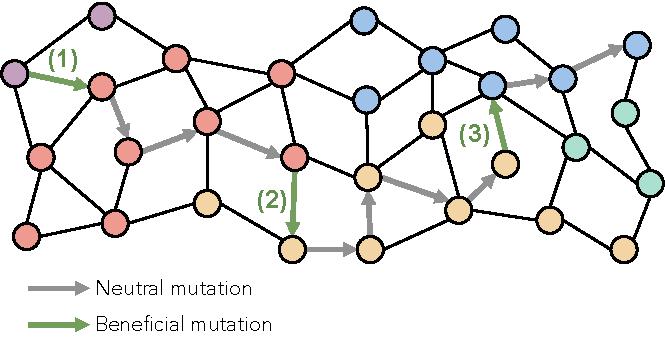
\includegraphics[width=0.7\textwidth]{generalintroduction_introduction_fig3.pdf}
\caption[Evolution on the genotype network for a robust organism.]{{\bf Evolution on the genotype network for a robust organism.} Each genotype is represented by a node, colored according to its fitness. Single mutations linking genotypes together generate a network, explored by evolving populations of organisms. The successive fixed mutations are represented by a path on this network. Beneficial mutations are represented by green arrows, while neutral ones are represented by grey arrows. Here, the evolutive path is composed by long successive travelling sessions on the neutral network, punctuated with three beneficial mutations (inspired from \citealt{wagner-2008b})}
\label{fig:general_introduction:introduction:fig3}
\end{figure}

%%%%%%%%%%%%%%%%%%%%%%%%%%

\subsection{Open-endedness}
The notion of open-endedness has been extensively discussed in \cite{banzhaf-et-al-2016}. Often defined as the ability to continuously produce novelty and/or complexity, open-endedness is a quite fuzzy notion. Considered as an important modeling challenge in the field of artificial life, the term is almost unknown in theoretical biology. Indeed, this recent concept still needs to be properly defined. According to \cite{banzhaf-et-al-2016}, open-endedness is essentially a \textbf{modeling concept}, and can refer to the capacity of a model to generate ``novelty''. \cite{banzhaf-et-al-2016} identified three types of novelties, depending on model capabilities: \textbf{variation}, \textbf{innovation} and \textbf{emergence}:

\begin{enumerate}
\item[\textbf{(1)}] \textbf{Variation.} A variation is defined here as a change to the values of a variable, or an instance in the model. This means that variations are simply the exploration of the predefined space of the model (``\textit{novelty in the model}'', \citealt{banzhaf-et-al-2016}). This definition could correspond to the notion of variability presented above;
\item[\textbf{(2)}] \textbf{Innovation.} An innovation is a change to the model itself. Hence, an innovation modifies the space in which variation can operate (``\textit{novelty that changes the model}'', \citealt{banzhaf-et-al-2016}). This definition could correspond to the notion of innovation discussed above;
\item[\textbf{(3)}] \textbf{Emergence.} Emergence is a change to the ``meta-model''. Indeed, a model is the instantiation of a conceptual model, defining types of objects and their relationships (``\textit{novelty that changes the meta-model}'', \citealt{banzhaf-et-al-2016}). This idea is exemplified by \cite{andrews-et-al-2011}: collective behavior (\textit{e.g.} collective bird fly) is often modeled by a class of individual-based models known as flocking or boids models \citep{reynolds-1987}. It is first needed to define the behavior of the boids (to define the agents), and then to collect individual positions (to collect data) in order to detect flockness (to measure the data). Then, a meta-model of a flocking model is the association of the concepts of agent, data and measure \citep{andrews-et-al-2011}. The notion of emergence directly refers to \textbf{major transitions}. According to \cite{smith-szathmary-1997}, a major transition occurs when ``\textit{entities that were capable of independent replication before the transition can only replicate as parts of a large unit after it}''. The comprehension of this property of living organisms is an important challenge for evolutionary biologists.
\end{enumerate}

We see that the concepts of variability, evolvability, robustness and open-endedness are intertwined in a complex way. Their evolution also require interdependencies between many mechanisms and properties, at multiple levels of biological organization.

%%%%%%%%%%%%%%%%%%%%%%%%%%%%%%%%%%%%%%%%%%%%%%%%
%%%%%%%%%%%%%%%%%%%%%%%%%%%%%%%%%%%%%%%%%%%%%%%%
\section{Capturing the whole spectrum of EvoEvo, or the necessity to build multi-level models}
\label{sec:general_introduction:introduction:evoevo_is_multilevel}

%%%%%%%%%%%%%%%%%%%%%%%%%%

\subsection{Modeling choices and the experimental method}
Building a model is a tough task, since modeling choices depend on the scientific question, but also on the kind of desired output (consciously or not) and maybe on some intuition. On this point, the modeling work presented in this manuscript has been largely influenced by the approach of the INRIA-Beagle team, in particular the works of \cite{knibbe-2007} and \cite{beslon-2008} on the modeling of complex biological systems.
A model is always false, and implies unavoidable assumptions, simplifications and shortcuts \citep{banzhaf-et-al-2016}. But more than that, when a model is correctly used to produce a new hypothesis or theory, this hypothesis or theory should acquire its own existence, independently from the model \citep{grimm-1999}. In this sense, the model is useful to generate new ideas, but should then disappear in their shadow \citep{beslon-2008}.

According to \cite{servedio-et-al-2014}, in evolutionary research, as in many other fields, some models are conceived to test the logic of verbal explanations of a theory, in the same way that empirical data is used to test scientific hypotheses. To build such a \textbf{proof-of-concept model}, we should follow the four steps of the \textbf{experimental method} promoted by Claude Bernard: \textbf{(i)} First, observe the nature and build hypotheses. \textbf{(ii)} Then, pick assumptions and build a model. \textbf{(iii)} Third, analyze the model, and finally \textbf{(iv)} evaluate new hypotheses and propose new directions, closing the loop (Fig. \ref{fig:general_introduction:introduction:fig4}). Even if the reality of scientific modeling has been shown to be more complex (the four steps are often interconnected, and even self-connected, such that building a model consist in navigating between them, \citealt{chalmers-1990,beslon-2008}), we should stick to this ``best practice'' guideline as much as possible. The hardiest task (but also the most exciting) probably consists in picking the right assumptions and build the model.

There is no well-defined guideline to pick the modeling assumptions, and to adjust the complexity of the model. However, depending on the scientific question, the model must at least represent the objects of interest, and their interactions. Regarding the study of EvoEvo, two important theoretical objects summarize the relationship between an evolving organism and its environment: \textbf{the genotype-to-phenotype map}, and the \textbf{fitness landscape}:

\begin{enumerate}
\item[\textbf{(1)}] \textbf{The genotype-to-phenotype map.}
The phenotype of an organism results from a complex and non-linear cascade of developmental, physiological and regulatory processes, summarized by the concept of genotype-to-phenotype map. According to the central dogma of molecular biology \citep{crick-1958}, the development of an organism reflects the flow of information from the genetic sequence to the phenotype. As such, the genotype-to-phenotype map is an object that represents all the functions of an organism (transcription, translation, regulation, protein folding, metabolism, environmental sensing, and so on). Hence, the genotype-to-phenotype map is generally a very complex object, an important condition to the evolution of evolution, as discussed above.
\item[\textbf{(2)}] \textbf{The fitness landscape.}
The fitness landscape is considered as one of the most important concepts in theoretical evolutionary biology. The fitness landscape projects the space of all possible genotypes, or phenotypes of a population of organisms in the space of fitness values, usually through a fitness function. Firstly used by \cite{wright-1932}, the fitness landscape is at the heart of historical models of evolution, such as \textbf{Fisher's geometric model} \citep{fisher-1930} or \textbf{NK-fitness landscapes model} \citep{kauffman-levin-1987}. The latter has been used to show how the complexity of a landscape influences the course of an evolutionary process \citep{correia-fonseca-2007}. The former will be presented in detail in part \ref{part1} of this manuscript. Often represented by a smooth function (\textit{e.g.}, a Gaussian-shaped function in Fisher's geometric model), the fitness landscape of living organisms is probably a much more complex, fluctuating and highly dimensional landscape (as discussed below).
\end{enumerate}

\begin{figure}[!ht]
\centering
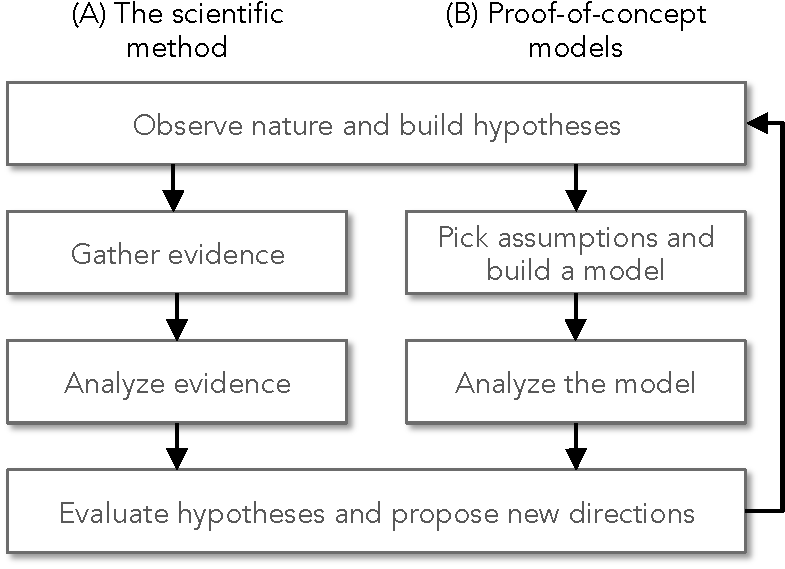
\includegraphics[width=0.6\textwidth]{generalintroduction_introduction_fig4.pdf}
\caption[Proof-of-concept modeling and the scientific method.]{{\bf Proof-of-concept modeling and the scientific method.} This flowchart shows the steps in the scientific process, with a parallel between the scientific method, as defined by C. Bernard, and proof-of-concept modeling methodology. (A) The main steps of the scientific method. (B) The steps of proof-of-concept modeling (inspired from \citealt{servedio-et-al-2014}).}
\label{fig:general_introduction:introduction:fig4}
\end{figure}

%%%%%%%%%%%%%%%%%%%%%%%%%%

\subsection{The necessity of multi-level modeling of evolution}
Computational models have been used to study evolution since the beginning of the 1990's \citep{adami-2006}. However, since then, most computational models used a partial representation of the genotype-to-phenotype map, generally in a fixed, predefined, fitness landscape. Yet, fitness is the result of the interaction of all the biological structures of an organism, including its interactions with the environment. Similarly, the variability/robustness/evolvability/open-endedness of the phenotype is the result of the interaction of variability/robustness/evolvability/open-endedness of all the biological structures of an organism, including its interactions with its environment. Furthermore, these properties are co-dependent and they may interact in a cooperative or competitive way (\textit{e.g.}, evolving chaperone proteins reduce phenotypic variability, thereby increasing robustness). Moreover, both the genotype-to-phenotype map and the fitness landscape are very likely to change during the course of evolution. That is why a computational model of EvoEvo must be multi-level, including the main organization levels of the genotype-to-phenotype map and the fitness landscape (genome, transcription network, metabolic network, phenotype, fitness, population, environment, and so on).

First, the genotype-to-phenotype map has long been considered as a one-directional and deterministic process, the genetic information flowing from the genotype to the phenotype. However, the development of living organisms is a non-deterministic process, depending on many molecular mechanisms that are fundamentally stochastic, as demonstrated by the stochastic nature of gene expression \citep{elowitz-et-al-2002}. Thus, one genotype can lead to several random phenotypes, and this stochastic variability can itself evolve through the genotype-to-phenotype map, as discussed in part \ref{part1} of this manuscript. Moreover, the information can flow back from the phenotype to the genotype (\textit{e.g.}, thanks to RNA interference, genetic regulation, or environment influence). Altogether, these mechanisms make the genotype-to-phenotype map of an organism a very complex object to analyze, generating non-intuitive situations through evolution of evolution.

Second, the fitness landscape of living organisms is much more complex than suggested in early models of evolutionary biology. The fitness of an organism depends on its environment. However, organisms constantly interact with it (including other organisms), such that the fitness landscape is constantly fluctuating, triggering complex evolutionary outcomes, such that co-evolution, niche construction, resource cycling, and ultimately major transitions. Some authors use the concept of \textbf{fitness seascape} to render the effect of fluctuating fitness landscapes on evolution \citep{mustonen-lassig-2009}.

As a whole, we see that the genotype-to-phenotype map and the fitness landscape form a complex system, which cannot be modeled statically as it is the case in classical mathematical representations \citep{fisher-1930,kauffman-levin-1987} (even the number of dimensions in the fitness landscape and in the genotype-to-phenotype map are evolvable). Moreover, both the genotype-to-phenotype map and the fitness landscape interact through evolution, a condition for evolution of evolution. For these reasons, a model of evolution of evolution should necessarily include complex, multi-layered and evolvable genotype-to-phenotype map and fitness landscape. Such a model will incorporate a large set of parameters and its study is likely to be very difficult. But as a compensation, it will give rise to new hypotheses and predictions, impossible to obtain with previous models.

%%%%%%%%%%%%%%%%%%%%%%%%%%

\subsection{But ...}
Based on the previous arguments, one could argue that our modeling approach should be exclusively a computational multi-scale approach, in the hope to observe the most complex features of EvoEvo; it would be foolish to do so. \textbf{(i)} The first reason is that history of theoretical evolutionary biology demonstrated the importance of mathematical models to understand evolution. From mendelian genetics to population genetics, quantitative genetics, coalescence theory, and so on, mathematical models remain the most powerful---and convincing---scientific tools. \textbf{(ii)} The second reason is that when the intuition of an hypothesis or a theory is acquired by the exploitation of a computational model of evolution, the best practice would be to derivate the mathematical equations representing the phenomenon in a more abstract way, and provide a robust mathematical analysis, if possible. This is for example the case for {\aevol} model \citep{knibbe-et-al-2007a} (presented below): in {\aevol}, a strong correlation between the genome size of bacterial-like digital organisms and their mutation rates has been identified. This observation has further been generalized with a more abstract mathematical model \citep{fischer-et-al-2014}.
\textbf{(iii)} The third reason is more practical: if some properties of EvoEvo can be studied with mathematical models, there is no reason not to do it \citep{peck-2004}. The approach used in this manuscript mostly results from this last reason. We decided to have a complementary approach, anchored in the modeling practice of the INRIA-Beagle team, using both sustainable mathematical and complex multi-scaled and individual-based approaches, as exemplified in the next parts of this manuscript.

%%%%%%%%%%%%%%%%%%%%%%%%%%%%%%%%%%%%%
%%%%%%%%%%%%%%%%%%%%%%%%%%%%%%%%%%%%%
\section{State of the art}
\label{sec:general_introduction:introduction:state_of_the_art}

We have seen above that the study of EvoEvo requires the use of a variety of models, including mathematical and multi-scaled individual-based approaches. In both cases, many models, with sometimes a long history behind them, already allowed to largely highlight the evolutive interactions between the genotype-to-phenotype map and the fitness landscape. Two modeling approaches will be presented below, and then be used as a basis to decipher some aspects of EvoEvo: \textbf{(i) Fisher's geometric model}, an historical mathematical model of the genetic theory of adaptation, and \textbf{(ii) digital genetics} formalism, that led to an experimental method in evolutionary modeling: \textbf{in silico experimental evolution}.

%%%%%%%%%%%%%%%%%%%%%%%%%%

\subsection{Fisher's geometric model of adaptation}

Fisher's geometric model (FGM, \citealt{fisher-1930}) has a long and interesting history (reviewed in \citealt{orr-2005,tenaillon-2014}), and received renewed interest in the last decades. According to \cite{tenaillon-2014}, a reason is that behind its apparent simplicity and limited number of parameters, FGM integrates a full model of mutations and epistatic interactions, with surprising emergent properties.

In FGM, each phenotypic character of an organism is represented by an axis in a Cartesian coordinate system. R.A. Fisher used the term \textbf{phenotypic complexity} to refer to the dimensionality $n$ of this space. Let's define the phenotype of an organism with $n$ characters by a point $\boldsymbol{z} = (z_1, z_2, ..., z_n)^T$ ($T$ being the matrix transposition operator). The fitness $W(\boldsymbol{z})$ of this organism is then determined by its distance to the fitness optimum $\boldsymbol{z_{opt}}$, such that:
\begin{equation}
W(\boldsymbol{z}) = exp \left[ -(\boldsymbol{z}-\boldsymbol{z_{opt}})^T \boldsymbol{\Sigma}^{-1} (\boldsymbol{z}-\boldsymbol{z_{opt}})\right]
\end{equation}
where $\boldsymbol{\Sigma}$ denotes a $n \times n$ positive-definite and symmetrical matrix defining the shape of the fitness landscape. For the sake of simplicity, an isotropic fitness landscape is usually assumed, meaning that fitness varies independently and in the same proportion for all characters. The origin of the coordinate system is also used as the fitness optimum ($\boldsymbol{z_{opt}} = \boldsymbol{0})$, such that the fitness function is reduced to a simple Gaussian-shaped function:
\begin{equation}
W(d) = \exp \left[ -\dfrac{d^2}{2} \right]
\label{eq:fitness_function}
\end{equation}
with $d = \lVert \boldsymbol{z} \rVert$ the euclidean distance of the phenotype $\boldsymbol{z}$ from the fitness optimum. Mutations are represented by a random vector $\boldsymbol{r} = (r_1, r_2, ..., r_n)^T$ moving the ancestral phenotype $\boldsymbol{z}$ to its offspring $\boldsymbol{z'}$ such that $\boldsymbol{z'}=\boldsymbol{z}+\boldsymbol{r}$. The probability distribution of the mutants is often characterized by a multivariate normal distribution of the form:
\begin{equation}
p(\boldsymbol{r}) = \dfrac{1}{\sqrt{(2\pi)^n|\boldsymbol{\Sigma_r}|}} \exp \left[ -\dfrac{1}{2}\boldsymbol{r}^T \boldsymbol{\Sigma_r}^{-1} \boldsymbol{r} \right]
\end{equation}
with $\boldsymbol{\Sigma_r}$ a covariance matrix. Thus, a mutation can potentially modify every characters, a property known as the \textbf{universal pleiotropy assumption} \citep{wagner-and-zhang-2011}. Usually, initial conditions are a maladapted clonal population of asexual organisms, sitting at a certain distance from the optimum $\boldsymbol{z_{opt}}$. Then, the work consists in studying the bout of adaptation towards the optimum. FGM implies some well-known assumptions, as described in details in \cite{martin-2014}: \textbf{(i)} the distribution of all random variables have finite mean and variance and satisfy Lindeberg's conditions (the central limit theorem can be applied), \textbf{(ii)} the fitness function is twice differentiable and admits at least one non-degenerate optimum, \textbf{(iii)} mutations have mild effects on the phenotype (mutational events remain ``local''), \textbf{(iv)} each mutation potentially affect every characters (the universal pleiotropy assumption), and \textbf{(v)} the variety of mutants is very large, such that quantitative characters vary continuously (the infinite-alleles approximation).

For a given phenotype $\boldsymbol{z}$, \cite{fisher-1930} demonstrated that the probability $P_a(x)$ that a random mutation of a given phenotypic size $s$ is favorable is $1-\Phi(x)$, where $\Phi$ is the cumulative distribution function of a standard normal random variable, and $x$ is a standardized mutational size $x = s\sqrt{n}/(2d)$. $n$ is the number of characters and $d = \lVert \boldsymbol{z} \rVert$ is the euclidean distance to the optimum. As shown in Figure \ref{fig:general_introduction:introduction:fig5}A, this probability quickly decreases with the mutational size.

R.A. Fisher also suggested that organisms may pay a cost for the complexity of their phenotype (the complexity being defined here as the number of characters $n$ under selection), because the probability to fix a beneficial mutation of a certain size literally vanishes when the number of characters increases \citep{orr-2000}. In consequence, only mutations with a very small size should segregate in a population. R.A. Fisher argued that his result was a demonstration of a \textbf{micro-mutationism} view of evolution, populations evolving smoothly by very little steps. However, R.A. Fisher omitted to consider that mutations occur in populations of finite size. As later demonstrated by M. Kimura with the neutral theory of evolution, new mutations appearing in a population have a significative chance to be lost at random, especially when their beneficial value is low. Thus, according to the cost of complexity and the effects of genetic drift, we should expect that only mutations of an intermediate size would segregate in an evolving population. Finally, as discussed by \cite{orr-2005}, evolution towards a fitness optimum cannot be reduced to the study of a single mutational event. When the entire boot of adaptation towards the fitness optimum is scrutinized in FGM, it appears that the size of fixed mutations depends on the distance from the optimum: very few large mutations are usually necessary to approach the fitness optimum, the remaining distance being filled with many small mutations, as shown in Figure \ref{fig:general_introduction:introduction:fig5}B.

\begin{figure}[!ht]
\centering
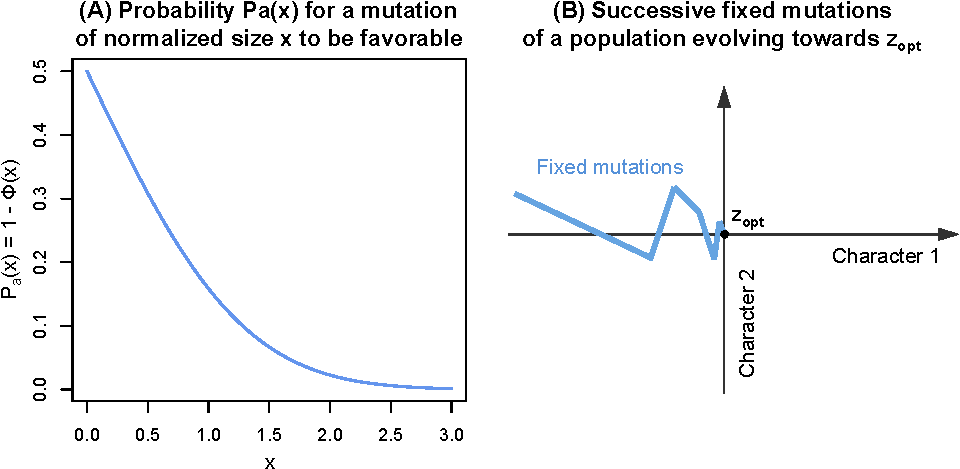
\includegraphics[width=0.9\textwidth]{generalintroduction_introduction_fig5.pdf}
\caption[The beneficial value of a mutation in FGM depends on its size.]{{\bf The beneficial value of a mutation in FGM depends on its size.}
\textbf{(A)} The probability $P_a(x)$ for a mutation of normalized size $x = s\sqrt{n}/(2d)$ (with $n$ the number of characters, and $d = \lVert \boldsymbol{z} \rVert$ the euclidean distance from the fitness optimum) to be favorable is $P_a(x) = 1-\phi(x)$ (blue curve). \textbf{(B)} When a population evolves towards the fitness optimum $\boldsymbol{z_{opt}}$, a few number of large mutations are usually sufficient to approach $\boldsymbol{z_{opt}}$. Then, a lot of small mutations are necessary to reduce this distance to zero, as shown in blue (inspired from \citealt{orr-2005}).}
\label{fig:general_introduction:introduction:fig5}
\end{figure}

%%%%%%%%%%%%%%%%%%%%%%%%%%

\subsection{In silico experimental evolution: a tool to study evolution}
\textit{In silico} experimental evolution \citep{hindre-et-al-2012,mozhayskiy-tagkopoulos-2013,batut-et-al-2013} is an approach based on the usage of individual-based models to evolve \textbf{digital organisms} in a computer, a field known as \textbf{digital genetics}. In digital genetics models \citep{adami-2006}, organisms are modeled by data-structures representing their genotype. The kind of structure used depends on the studied level(s) of organization (numerical vectors, binary sequences, regulation network, ...) and the formalism used to develop the model (reviewed in \citealt{mozhayskiy-tagkopoulos-2013,hindre-et-al-2012}). As discussed in part \ref{part2} of this manuscript, the development of an \textit{in silico} model of evolution needs some ``ingredients''. The minimum requirement is the \textbf{evolutionary engine} enabling the data-structures to reproduce, mutate and be selected depending on a fitness function. Many digital genetics models have been proposed in the literature, Avida being the best known \citep{wilke-et-al-2001,adami-2006}. However, only a few models are able to efficiently address questions related to evolution of evolution, in particular because most formalisms impose that the structure of organisms and the fitness landscape are fixed over time.

The increasing number of parameters and the computational and time resources needed to run multi-scale individual-based simulations forbid an exhaustive and rigorous exploration of the parameters and state spaces of the system, as it could be the case for Fisher's geometric model for example.
Hence, an \textbf{experimental approach} is needed to study this kind of models. According to \cite{peck-2004}, complex simulation models should be explored with the same experimental and statistics tools used for real systems:
\begin{quote}
Simulations are experimental systems. Their complexity can make them closer cousins in complexity to nature itself than to simple analytic models, but with a powerful advantage over the real world: the modeler has complete control of the system \citep{peck-2004}.
\end{quote}
In evolutionary biology, the experimental method that consists in studying evolving organisms is \textbf{experimental evolution}. In experimental evolution, fast replicating micro-organisms (\textit{e.g.}, bacteria or viruses) are being evolved in controlled environments for thousands of generations \citep{philippe-2007}. It is then possible to recover precisely the evolutionary history of lab strains by reviving frozen samples \citep{elena-and-lenski-2003}. However, despite its explanatory and statistical power, experimental evolution remains a long and costly process. \textbf{In silico experimental evolution} (ISEE) consists in mimicking this process with digital organisms \citep{hindre-et-al-2012,mozhayskiy-tagkopoulos-2013,batut-et-al-2013}, as shown in Figure \ref{fig:general_introduction:introduction:fig6}: ancestral microbial (or digital) populations are evolved in controlled environments and regularly frozen (or saved in a backup), independent repetitions are made, and frozen populations can be revived (or reloaded in memory) to perform competition experiments and other analyses. ISEE approach while be exemplified in the part \ref{part2} of this manuscript.

\begin{figure}[!ht]
\centering
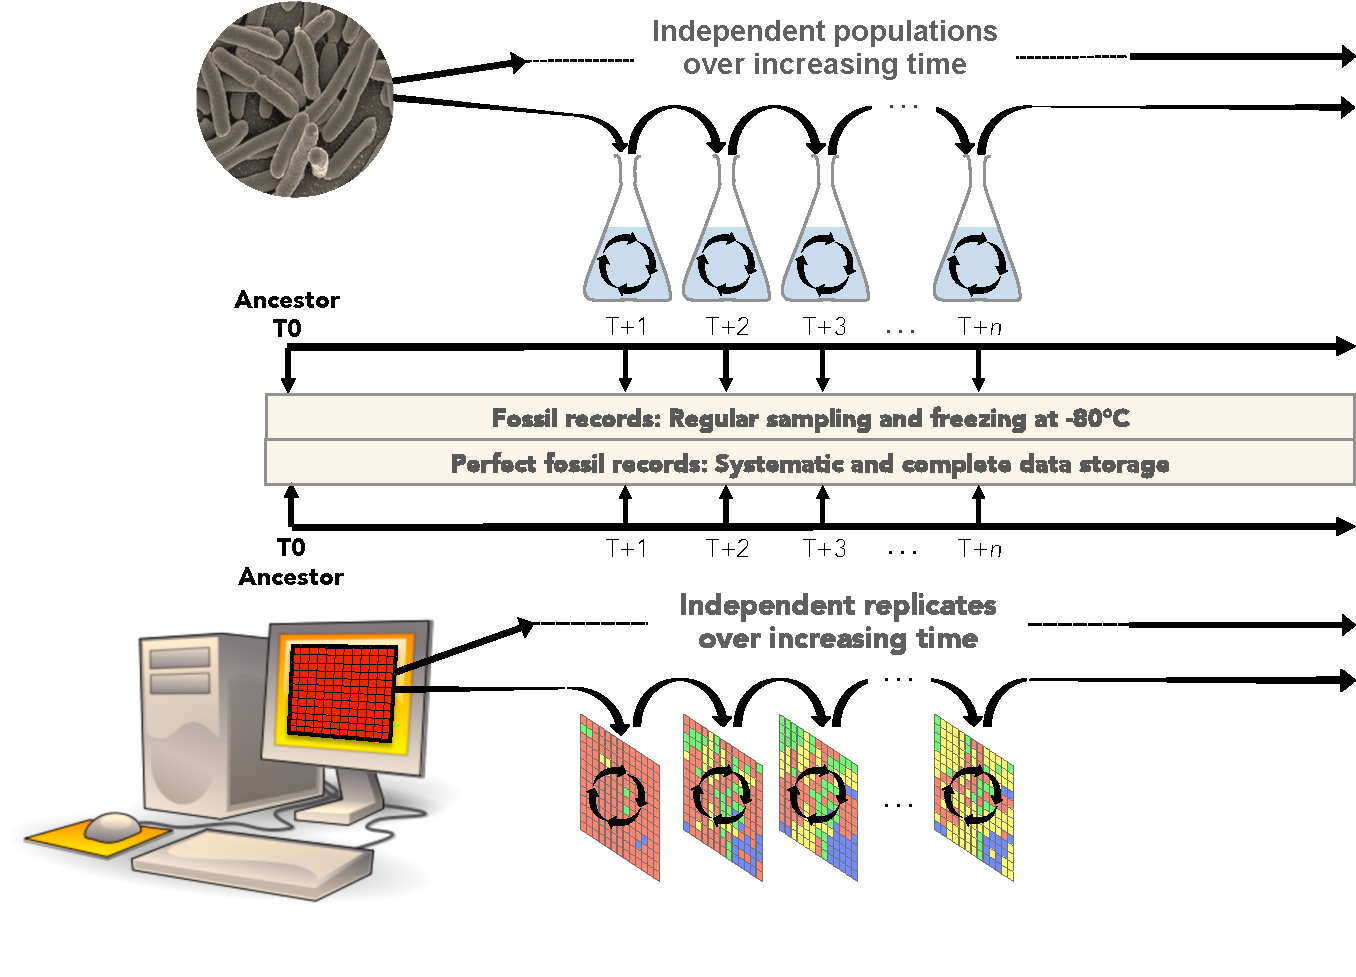
\includegraphics[width=1\textwidth]{generalintroduction_introduction_fig6.pdf}
\caption[In vivo and in silico evolution experiments.]{{\bf In vivo and in silico evolution experiments.}
Ancetral real micro-organisms (top) and digital organisms (bottom) are propagated in controlled environments, in a laboratory or in a computer respectively. Wet or digital populations are regularly frozen, or saved in backups, respectively and can be revived or reloaded at any time.
Many replicate populations can be independently evolved from a common ancestor T0 (inspired from \citealt{hindre-et-al-2012}).}
\label{fig:general_introduction:introduction:fig6}
\end{figure}

Two formalisms have recently been used to develop computational models allowing for \textit{in silico} experimental evolution. \cite{knibbe-et-al-2007a,knibbe-et-al-2007b} used the \textbf{sequence-of-nucleotides} formalism to develop {\aevol} software. With this model, the authors showed that indirect selection could select specific genetic and network structures depending on the mutational and selective pressures \citep{knibbe-et-al-2007b,beslon-et-al-2010a,beslon-et-al-2010b}. In parallel, \cite{crombach-hogeweg-2008} developed the \textbf{pearls-on-a-string} formalism and used it to show that, in time-varying environments, regulation networks, metabolic networks and species networks can acquire structures that increase the evolvability of the organisms \citep{crombach-hogeweg-2007,crombach-hogeweg-2008,crombach-hogeweg-2009}. These two formalisms are described in the next sections.

%%%%%%%%%%%%%%%%%%%%%%%%%%

\subsection{The sequence-of-nucleotides formalism}
In the sequence-of-nucleotides formalism, the genome is a variable-length string of characters. Predefined signal sequences, analogous to promoters, terminators or start/stop codons, are used to detect genes. Therefore, mutational processes, such as point mutations, small insertions and deletions, or large rearrangements can be simulated in a realistic manner \citep{hindre-et-al-2012}. The sequence-of-nucleotides formalism has been successfully used to study \textit{e.g.}, the evolution of non-coding DNA and the genes number \citep{knibbe-et-al-2007b}, the evolution of the size and topology of gene networks \citep{kuo-et-al-2006,beslon-et-al-2010a}, gene network interference \citep{mattiussi-floreano-2007,marbach-et-al-2009}, the evolution of ``public good'' production \citep{frenoy-et-al-2013}, and the reduction of genome size in some species \citep{batut-et-al-2013}.

Here, we will focus on the {\aevol} software \citep{knibbe-et-al-2007a}, because we will get inspired from its genome and genetic regulation representations in the following. In {\aevol}, each digital organism owns a circular, double-stranded chromosome (Fig. \ref{fig:general_introduction:introduction:fig7}a) that is actually a string of binary nucleotides, 0 being complementary of 1 and reciprocally. This chromosome contains coding sequences (genes) separated by non-coding regions. Each coding sequence is detected by a transcription-translation process and decoded into a ``protein'' able to contribute positively or negatively to a range of abstract quantitative characters (Fig. \ref{fig:general_introduction:introduction:fig7}a). The mechanisms of transcription and translation are modeled in detail (Fig. \ref{fig:general_introduction:introduction:fig7}b,c,e), depending on a genetic code (Fig. \ref{fig:general_introduction:introduction:fig7}d). The combination of all proteins yields the value of each abstract phenotypic character (Fig. \ref{fig:general_introduction:introduction:fig7}g). Adaptation is then measured by comparing the phenotypic values to an arbitrary set of target values. The most adapted individuals have higher chances of reproduction. When a chromosome is replicated, it can undergo point mutations, small insertions and small deletions, but also large chromosomic rearrangements: duplications, large deletions, inversions, and translocations. The various types of mutations can modify existing genes, but also create new genes, delete some existing genes, modify the length of the intergenic regions, modify gene order, and so on.

\begin{figure}[!ht]
\centering
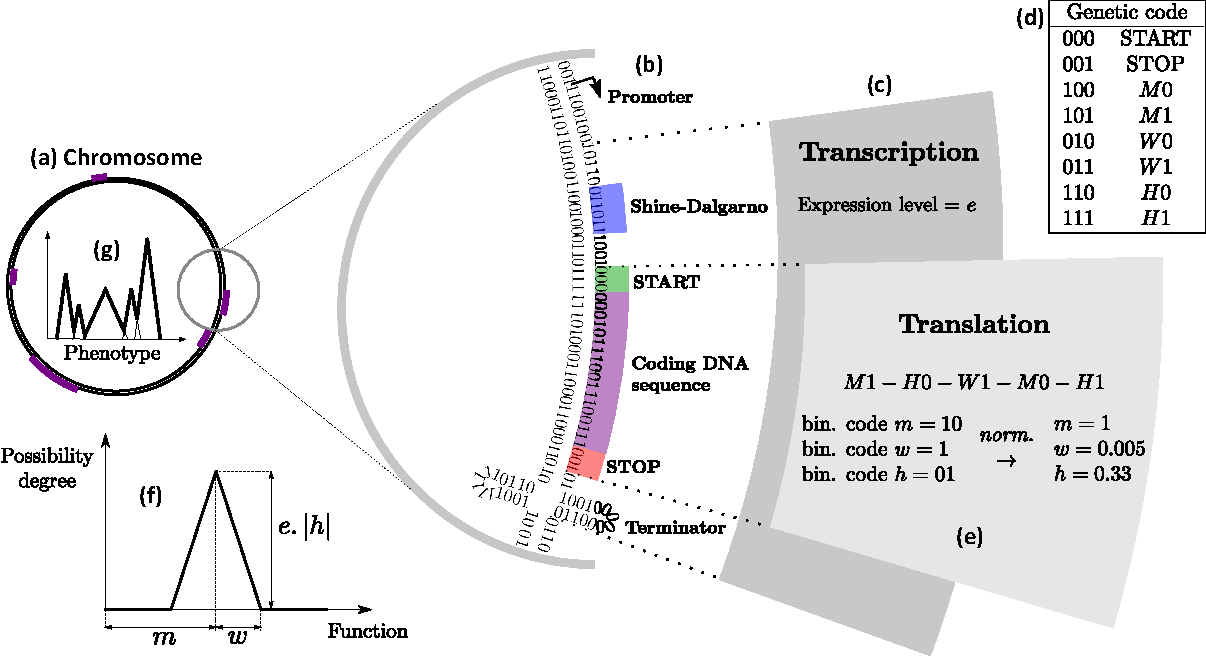
\includegraphics[width=1\textwidth]{generalintroduction_introduction_fig7.pdf}
\caption[A description of {\aevol} model.]{{\bf A description of {\aevol} model.}
In the model, each organism owns a circular double-stranded binary chromosome \textbf{(a)} along which genes are delimited by predefined signal sequences \textbf{(b)}. Promoters and terminators mark the boundaries of RNAs \textbf{(c)} within which coding sequences are in turn identified between a Shine-Dalgarno-START signal and an in-frame STOP codon. Each coding sequence is then translated into a protein sequence using a predefined genetic code \textbf{(d)}. This protein sequence is decoded as three real parameters called m, w and h \textbf{(e)}. Proteins, phenotypes and environments are represented similarly through mathematical functions that associate a level to each abstract phenotypic character in [0, 1]. The contribution of a protein is a piecewise-linear function with a triangular shape, with position $m$, half-width $w$ and height $h$ \textbf{(f)}. All proteins encoded in the chromosome are then combined to compute the phenotype \textbf{(g)}, which is compared to the environmental target to compute the fitness of the individual (inspired from \citealt{knibbe-parsons-2014}).}
\label{fig:general_introduction:introduction:fig7}
\end{figure}

{\aevol} model has been extended to include regulation of genetic expression, by adding a representation of cellular gene networks \citep{beslon-et-al-2010a}. This extended version of {\aevol}, named R-{\aevol}, is a model of prokaryotic regulation. To simulate the interactions between \textbf{transcription factors} and \textbf{promoters}, two \textbf{binding sites} are defined for each promoter. Located immediately before the promoter, the \textbf{enhancer site} increases the transcriptional activity when transcription factors bind to it. Directly following the promoter, \textbf{the operator site}, down-regulates the promoter's activity when a transcription factor binds to it. Each promoter $i$ owns a basal expression level $\beta_i$, which depends on how close its sequence is to a consensus sequence. The transcriptional activity of this promoter depends on the combined activity of the enhancer site activity $A_i$ and the operator site activity $O_i$, that read:
\begin{equation}
A_i(t) = \sum_j c_j(t)A_{ji}
\end{equation}
and:
\begin{equation}
O_i(t) = \sum_j c_j(t)O_{ji}
\end{equation}
with $A_{ji}$ (resp. $O_{ji}$) the affinity of protein $j$ for the enhancer site of the promoter $i$ (resp. for the operator site) and $c_j(t)$ the concentration of protein $j$ at time $t$.

The transcription rate $e_i(t)$ of the RNA sequence associated to the promoter $i$ is then given by the following Hill-like function:
\begin{equation}
e_i(t) = \beta_i \left( \dfrac{\theta^n}{O_i(t)^n+\theta^n} \right) \left( 1 + \left( \dfrac{1}{\beta_i}-1\right) \left( \dfrac{A_i(t)^n}{A_i(t)^n+\theta^n} \right) \right)
\end{equation}
where $n$ and $\theta$ are the two parameters defining the shape of the Hill-function. Finally, given the transcription rate, one can compute the protein concentration (for simplicity, it is assumed that the protein concentration is linearly proportional to the RNA concentration) through the following synthesis-degradation rule:
\begin{equation}
\left\{
\begin{array}{rcl}
c_i(0) & = & \beta_i/\phi\\\\
\dfrac{d c_i}{d t} & = & e_i(t) - \phi c_i(t)
\end{array}
\right.
\end{equation}
where $\phi$ is a temporal scaling constant representing the protein degradation rate. Thus, when a gene is regulated, the concentration of its product is scaled up or down depending on its transcription rate.

%%%%%%%%%%%%%%%%%%%%%%%%%%

\subsection{The pearls-on-a-string formalism}

In the pearls-on-a-string formalism, the genome is a variable-length string of ``pearls'' of different types: phenotype genes, transcription factor genes, repeats, retrotransposons, binding sites, and so on. Each pearl type can exist in a predefined number of variants. Mutational operators (point mutations, rearrangements) can modify the genes number, the order of the pearls and the regulation. The pearls-on-a-string formalism has been successfully used for the study of genome and network evolvability \citep{crombach-hogeweg-2007,crombach-hogeweg-2008}, resource processing in ecosystems \citep{crombach-hogeweg-2009}, and sympatric speciation \citep{tentussscher-hogeweg-2009}.

Recently, \cite{cuypers-hogeweg-2012} developed a multi-scale model based on the pearls-on-a-string formalism: the Virtual Cell model.
As shown on Figure \ref{fig:general_introduction:introduction:fig8}, in Virtual Cell model, digital organisms own circular genomes made of ``pearls'', encoding for five types of proteins. Organisms grow on an externally provided resource $A$ (Fig. \ref{fig:general_introduction:introduction:fig8}a), by pumping it (Fig. \ref{fig:general_introduction:introduction:fig8}b) or by passive diffusion through the cell's membrane (Fig. \ref{fig:general_introduction:introduction:fig8}c). The pumps require the consumption of an energy carrier molecule $X$, enzymatically produced from $A$ by a catabolic reaction (Fig. \ref{fig:general_introduction:introduction:fig8}d). Both $A$ and $X$ molecules are required to build end products via another enzymatic reaction (Fig. \ref{fig:general_introduction:introduction:fig8}e). Two other protein types are transcription factors that up-regulate or down-regulate the production of proteins depending on the effect of their ligands, $A$ or $X$ (Fig. \ref{fig:general_introduction:introduction:fig8}f). With their model, \cite{cuypers-hogeweg-2012} proposed that the complex genotype-to-phenotype map of digital organisms drives genome size dynamics, due to an emerging interplay between adaptation, neutrality, and evolvability, showing that genome expansion and streamlining are generic patterns of evolving systems. More recently, \cite{cuypers-et-al-2017} shown with the Virtual Cell model that depending on the frequency of environmental changes, digital organisms evolve different adaptive strategies: when the change frequency is low, evolution leads to phenotypic plasticity, while when the change is high, evolution leads to enhanced evolvability.

\begin{figure}
\centering
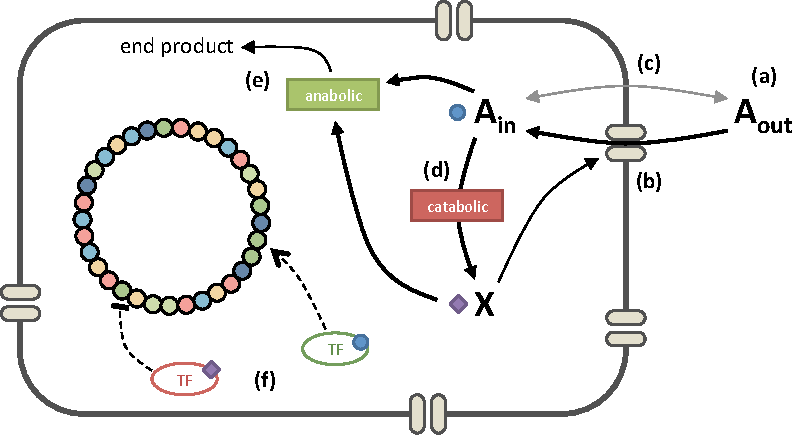
\includegraphics[width=1\textwidth]{generalintroduction_introduction_fig8.pdf}
\caption[A description of the Virtual Cell model.]{{\bf A description of the Virtual Cell model.}
In Virtual Cell model, digital organisms own circular genomes made of ``pearls'', encoding for five types of proteins. Organisms grow on an externally provided resource $A$ \textbf{(a)}, by pumping it \textbf{(b)} or by passive diffusion through the cell's membrane \textbf{(c)}. The pumps require the consumption of an energy carrier molecule $X$, enzymatically produced from $A$ by a catabolic reaction \textbf{(d)}. Both $A$ and $X$ molecules are required to build end products via another enzymatic reaction \textbf{(e)}. Two other protein types are transcription factors that up-regulate or down-regulate the production of proteins depending on the effect of their ligands, $A$ or $X$ \textbf{(f)} (inspired from \citealt{cuypers-hogeweg-2012}).}
\label{fig:general_introduction:introduction:fig8}
\end{figure}

%%%%%%%%%%%%%%%%%%%%%%%%%%%%%%%%%%%%%%%%
%%%%%%%%%%%%%%%%%%%%%%%%%%%%%%%%%%%%%%%%
\section{An attempt to merge sequence-of-nucleotides and pearls-on-a-string formalisms}
\label{sec:general_introduction:introduction:bag_of_tuples}

%%%%%%%%%%%%%%%%%%%%%%%%%%
\subsection{A common formalism: the ``bag of tuples''}

The \textbf{sequence-of-nucleotides} and the \textbf{pearls-on-a-string} formalisms have a common property: while their genomic representation (the way information is stored in the genome) differ significantly, in both formalisms, a non-ordered set of tuples is extracted from the genomic data-structure: a \textbf{bag of tuples}.

A tuple is an ordered list $(x_1,x_2,...,x_n): T_1 \times T_2 \times ... \times T_n$ with $T_i$ the ``product type'' of $x_i$ (\textit{e.g.}, $\mathbb{R}$, $\mathbb{N}$,...). In both sequence-of-nucleotides and pearls-on-a-string formalisms, the genotype-to-phenotype map is based on the extraction of an unordered set of tuples from the genotype. This set of tuples is then used to build the higher organism level in another specified space. For example, {\aevol} uses a complex and non-linear artificial genetic code to extract a set of triplets $(m,w,h) \in \mathbb{R}^3$ from a circular and double-stranded binary sequence. In pearls-on-a-string models, the genome is an unordered list of tuples. Depending on the complexity of projection operators, the evolution on the genome structure and the genotype-to-phenotype map will not be the same. In both models, the order of the tuples does not impair the fitness, but, since the tuples are encoded locally in the genome (in coding regions, or in pearls), the modification of their order on the sequence can potentially affect long-term evolution, as demonstrated in \cite{knibbe-et-al-2007a,knibbe-et-al-2007b}.
 
%%%%%%%%%%%%%%%%%%%%%%%%%%
\subsection{Bags of tuples and artificial chemistries}

When developing a new individual-based model of evolution, one important task is to define an \textbf{artificial chemistry} for this model: how to represent the various bio-molecules (DNA, RNA, proteins, metabolites, and so on) and their interactions? Artificial chemistry (AChem) is an entire field of research \citep{dittrich-2001,banzhaf-yamamoto-2015}, which is not directly in the scope of this manuscript. However, it is important to define here the most basic steps necessary to develop an AChem:

An AChem can be defined as a triplet $(S,R,A)$, where $S$ is the set of all possible molecules, $R$ is a set of reaction rules representing the interactions among the molecules, and $A$ is an algorithm describing the reaction vessel or domain and how the rules are applied to the molecules inside the vessel \citep{dittrich-2001}. The set of molecules $S = \{s_1,s_2,...,s_n\}$ can potentially be infinite. A reaction rule $r \in R$ is a chemical equation:
\begin{equation}
s_1 + s_2 + ... + s_i \rightarrow s'_1 + s'_2 + ... + s'_j
\end{equation}
With the reactants (or the substrates) on the left side, and the products on the right side. $i$ is the order of the reaction. The set of reaction rules $R$ can be defined explicitly (all possible reactions $r$ are defined and are in finite number), or implicitly. In this example, stoichiometry is 1 for all reactants, but there is no constraint on this point. The algorithm $A$ is applied on an instance of $S$, that is, a collection $P$ of molecules. The set of chemical equations $R$ can be solved with stochastic or deterministic methods, possibly adding spatial rules.

From this simple definition, two ways to define an AChem in the bag-of-tuples formalism are possible in first instance (Fig. \ref{fig:generalintroduction:introduction:fig9}):
\begin{enumerate}
\item[\textbf{(1)}] Each tuple codes for a reaction rule. In this case, each organism $i$ owns a specific set of reactions rules $R_i$, somehow carrying its own artificial chemistry. For instance, a tuple $(x_1,x_2,...,x_n)$ could define the chemical equation of order $n/2$:
\begin{equation}
s_1 + s_2 + ... + s_{\frac{n}{2}} \rightarrow s_{\frac{n}{2}+1} + s_{\frac{n}{2}+2} + ... + s_n
\end{equation}
With $x_i \equiv s_i$ (Fig. \ref{fig:generalintroduction:introduction:fig9}.1).
\item[\textbf{(2)}] Each tuple codes for a chemical species, being potentially a reactant for a subset of reactions in $R$. In this case, $R$ is defined once for the whole system, a reaction occurring only if all the reactants are present. For instance, let's consider the set of reaction rules $R$ containing the reaction:
\begin{equation}
s_i + s_j \leftrightarrow s_i . s_j
\label{eq:reaction1}
\end{equation}
And the reaction:
\begin{equation}
s_i . s_j \rightarrow s_k + s_j
\label{eq:reaction2}
\end{equation}
With $s_i, s_j, s_k \in S$, and ``.'' symbolizing a chemical bound. Thus, a singleton $x_j \equiv s_j$ (a tuple of length 1) catalyzes the enzymatic reaction:
\begin{equation}
s_i + s_j \leftrightarrow s_i . s_j \rightarrow s_k + s_j
\label{eq:reaction3}
\end{equation}
To describe more precisely the reaction, it is also possible to replace the singleton $x_i$ by a pair $(x_j, c_j)$, with $c_j = [s_j]$. With this AChem, a tuple could encode a useless compound, if no other reactant is present (Fig. \ref{fig:generalintroduction:introduction:fig9}.2).
\end{enumerate}

\begin{figure}[!ht]
\centering
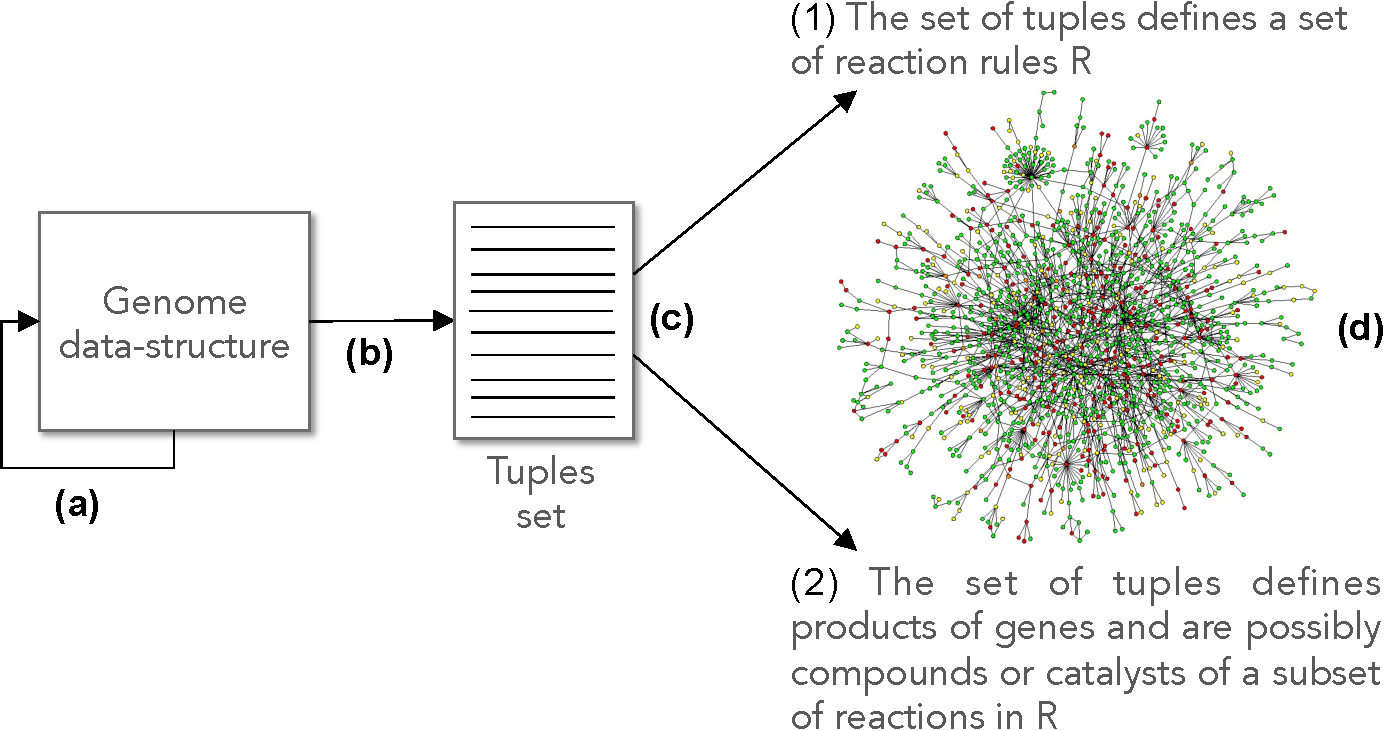
\includegraphics[width=0.7\textwidth]{generalintroduction_introduction_fig9.pdf}
\caption[A general framework for the bag-of-tuples formalism.]{{\bf A general framework for the bag-of-tuples formalism.}
\textbf{(a)} At each replication, the genome data-structure undergoes mutations (point mutations, large rearrangements, recombinations, horizontal transfers). \textbf{(b)} A mapping, often complex and non-linear, gives a non-ordered set of tuples (the bag of tuples). \textbf{(c)} Depending on modeling choices, the set of tuples defines: (1) an independent set of reactions rules $R$ in each organism, or (2) chemical products (proteins, catalysts, metabolites, ...) involved or not in a subset of reactions belonging to $R$. \textbf{(d)} The set of reaction rules defines the interactome of the organism (the biochemical network including all organism's reactions). On modeling purpose, this biochemical network can be splitted into several sub-networks (genetic regulation network, metabolic network, ...).}
\label{fig:generalintroduction:introduction:fig9}
\end{figure}

The bag-of-tuples formalism thus provides a general framework to encode an artificial chemistry with a genetic sequence. As shown in part \ref{part2}, we chose the modeling scheme \textbf{(1)} to define the artificial chemistry in our multi-scale model of evolution (Fig. \ref{fig:generalintroduction:introduction:fig9}.1).

%%%%%%%%%%%%%%%%%%%%%%%%%%%%%%%%
%%%%%%%%%%%%%%%%%%%%%%%%%%%%%%%%
\section{Outline}
\label{sec:general_introduction:introduction:outline}

To summarize, we have seen that the modeling approach needed to model and study EvoEvo is multi-faceted, but can efficiently use well-defined modeling formalisms available in the literature.

On the one hand, it is essential to extend previous mathematical models used in theoretical evolutionary biology to deal with some aspects of EvoEvo. The advantage of this approach is to provide robust predictions, often accompanied with analytical solutions and mathematical proofs. In the next part of this manuscript, this approach will be exemplified with an extended version of Fisher's geometric model accounting for the evolution of phenotypic noise (part \ref{part1}). With this model, we made promising predictions on the evolution of phenotypic noise in the face of phenotypic complexity.

On the other hand, we have seen that some of the most salient properties of EvoEvo emerge from multi-level evolution. The usage of a multi-scaled individual-based model of evolution, including a complex and evolvable genotype-to-phenotype map is required to tackle this complexity. Two formalisms have been independently developed with the ultimate goal to deal with some of the EvoEvo aspects: the sequence-of-nucleotides formalism and the pearls-on-a-string formalism. Moreover, a methodology has been specifically developed to study \textit{in silico} models of evolution: \textit{in silico} experimental evolution, that provides the same experimental tools than wet experimental evolution. In the second part of this manuscript, a multi-scale model of evolution merging these different formalisms will be presented. This model allowed us to study the evolution of niche construction and stable cross-feeding, and also the evolution of genetic regulation networks.






%%%%%%%%%%%%%%%%%%%%%%%%%% PART 1 %

\part{An extended version of Fisher's geometric model to study phenotypic noise}
\label{part1}


%%%%%%%%%%%%%%%
%%%      CHAPTER      %%%
%%%%%%%%%%%%%%%

\chapter{Phenotypic noise and the cost of complexity}
\label{ch:part1:sigmaFGM}

\paragraph{}
\paragraph{}
\paragraph{}
\paragraph{}
\paragraph{}
\paragraph{}
\paragraph{}
\paragraph{}
\begin{center}
\large \textbf{The results presented in this chapter have been submitted to the Evolution journal.}
\end{center}

%%%%%%%%%%%%%%%%%%%%%%%%% ABSTRACT %
\newpage

\begin{quote}
My Umi said shine your light on the world\\
Shine your light for the world to see\\
(Mos Def -- Umi Says, Black on Both Sides)
\end{quote}

\definecolor{grisclair}{rgb}{0.91,0.89,0.85}
\begin{center}
\colorbox{grisclair}{
\begin{minipage}[t]{0.9\textwidth}
\begin{center}
\large{\textbf{Abstract}}
\end{center}
Experimental studies demonstrate the existence of phenotypic diversity despite constant genotype and environment, and suggest that the intensity of this phenotypic noise could be evolvable. Theoretical models based on a single phenotypic character predict that during an adaptation event, phenotypic noise should be positively selected under directional selection, and then be reduced when the selection becomes stabilizing. However, it is unclear whether the (temporary) selective advantage of phenotypic noise would hold for more realistic, multidimensional phenotypes. Indeed, Fisher's geometric model of adaptation predicts a cost of complexity, where beneficial mutations become increasingly harder to fix as the number of phenotypic characters increases. Here, we extend Fisher's geometric model by adding an evolvable phenotypic noise. We show that the cost of complexity makes noise useless under directional selection, except if noise correlations between characters are evolvable. In this case, noise evolves to a specific configuration, with elevated noise towards the fitness optimum, and minimized noise in all other directions. Such an aligned noise speeds up adaptation and largely compensates for the cost of complexity. By analyzing published phenomic data of 37 yeast strains, we confirm the plausibility of intra-strain noise correlations between phenotypic characters.
\end{minipage}
}     
\end{center}

%%%%%%%%%%%%%%%%%%%%%%%%%%%%%%%%%%%%%%%%%
%%%%%%%%%%%%%%%%%%%%%%%%% SECTION : INTRODUCTION %
%%%%%%%%%%%%%%%%%%%%%%%%%%%%%%%%%%%%%%%%%

\section{Introduction}

The phenotype of an organism results from a complex and non-linear cascade of developmental, physiological and regulatory processes, formalized by the concept of \textit{genotype-to-phenotype map} \citep{alberch-1991}.
An increasing number of experimental studies demonstrated that the genotype-to-phenotype map is not a deterministic process and can generate phenotypic diversity \citep{symmons-and-raj-2016}, not explained by environmental interactions.
Indeed, isogenic populations having the same genotype and grown in the same environment sometimes exhibit a random distribution of phenotypes, a phenomenon known as \textit{phenotypic noise} \citep{yvert-et-al-2013}.
This observed phenotypic stochasticity is mainly due to the propagation of stochastic molecular events \citep{elowitz-et-al-2002,jo-et-al-2005,raser-and-oshea-2005,bahar-et-al-2006,dar-et-al-2014} through the genotype-to-phenotype map.

Recent experimental results have suggested that phenotypic noise can be tuned. \cite{yvert-et-al-2013} used single-cells phenomics \citep{ohya-et-al-2015} on different natural strains of yeast to measure hundreds of phenotypic characters. They showed that phenotypic noise is strongly dependent on the strain background and largely character-specific (specific strains showing elevated noise for subset of characters) but also global (a few strains displaying elevated noise for many unrelated characters). 
\cite{shen-et-al-2012} demonstrated the importance of ``variance-controlling genes'' controlling phenotypic variance in \textit{Arabidopsis thaliana}. \cite{boukhibar-and-barkoulas-2016} reviewed experimental results also demonstrating the existence of ``variance-amplifier loci'', ``phenotypic capacitors'', or ``master regulators'' controlling phenotypic noise on multiple characters \citep{levy-and-siegal-2008,lempe-et-al-2013}.

Theoretical and experimental results also tend to demonstrate that phenotypic noise has an impact on fitness. On the one hand, phenotypic noise appears to be deleterious for organisms facing a stable environment. Recently, \cite{keren-et-al-2016} demonstrated with an experimental study on \textit{Saccharomyces cerevisiae} that phenotypic characters sensitive to variation (\textit{i.e.}, having a sharp fitness function) exhibit low noise, in opposition to robust characters, that exhibit higher noise levels. \cite{mineta-et-al-2015} used a mathematical model from population genetics to demonstrate that elevated phenotypic noise reduces effective population size and enhances genetic drift, when the population is at the fitness optimum.
On the other hand, many experimental and theoretical studies demonstrated the positive role of phenotypic noise in several \textit{evolutionary stable strategies} (ESS) such as bet-hedging  \citep{kussell-and-leibler-2005,acar-et-al-2008,beaumont-et-al-2009,tsuru-et-al-2011}, stable mix and altruistic strategies \citep{dejong-et-al-2011}, or bacterial persistence \citep{balaban-et-al-2004}.
Phenotypic noise could also be exploited by organisms in stress responses \citep{chalancon-et-al-2012}. For example, \cite{charlebois-et-al-2014} showed with a mathematical model that regulatory network motifs can enhance drug resistance by transiently increasing isogenic cell-to-cell variability. \cite{holland-et-al-2014} measured variability on fitness-dependent phenotypic characters in natural populations of yeasts. They showed that populations living in a polluted environment develop high heterogeneity as a survival strategy against adverse conditions in the wild. Experimental studies on yeast also revealed that expression noise of essential genes \citep{newman-et-al-2006} (or ``dosage-sensitive'' genes, \citealt{fraser-et-al-2004}) is minimized to prevent harmful variations \citep{lehner-2008,wang-and-zhang-2011}. Moreover, ``stress-related'' genes (\textit{e.g.}, drug-resistance genes) often present high levels of expression noise \citep{fraser-and-kaern-2009,zhuravel-et-al-2010,charlebois-et-al-2011,charlebois-et-al-2014,charlebois-2015}. This phenomenon was demonstrated in laboratory experiments on \textit{Escherichia coli} \citep{ito-et-al-2009}, and on yeast \citep{liu-et-al-2015}.

Together, these studies support ``\textit{the possibility that, if noise is adaptive, microevolution may tune it in the wild. This tuning may happen on specific traits or by varying the degree of global phenotypic buffering}'' \citep{yvert-et-al-2013}. Phenotypic noise thus appears as a complex and evolvable phenotypic character, exploited in many survival strategies. However, while phenotypic noise has been demonstrated to be exploited by evolution in a variety of ESS, the possible role of an evolvable phenotypic noise in directional selection, when a population must adapt to a new environment, is poorly known.
A few studies examined the simple case of a single gene undergoing stochasticity of gene expression, and brought important insights. \cite{zhang-et-al-2009} suggested with a mathematical model of a single gene that elevated expression noise facilitates evolution in directional selection, because it enhances the probability to fix beneficial mutations. According to the authors, this facilitated evolution is only possible if the fitness function is convex (there is no advantage for elevated noise in the case of a linear or a concave fitness function). A recent experimental study on \textit{Saccharomyces cerevisiae} \citep{keren-et-al-2016} suggests that fitness landscapes related to gene expression present a variety of curvatures, among which convex, concave or linear forms.
The prediction of \cite{zhang-et-al-2009} has also been corroborated by a recent experimental study by \cite{bodi-et-al-2017}, that showed that phenotypic heterogeneity due to the stochasticity of gene expression enhances the adaptive value of beneficial mutations on a specific gene of \textit{Saccharomyces cerevisiae} in directional selection.

As stated by \cite{eldar-and-elowitz-2010}, ``\textit{based on these general results, one might expect increased phenotypic noise during periods of adaptation to new environments, followed by reduction in noise when selection becomes stabilizing}''. It is tempting to generalize results from single gene models to the level of an entire and complex phenotype undergoing phenotypic noise. However, this generalization is far from being straightforward. Indeed, the phenotype is the result of a complex and non-linear process involving the expression of tens on thousands of genes.
Fisher's geometric model of adaptation (FGM) has been specifically conceived to study the adaptation of complex phenotypes to a new environment. Using it, \cite{fisher-1930} suggested that organisms may pay a cost to the ``complexity'' of their phenotype, beneficial mutations becoming increasingly harder to fix when the number of phenotypic characters under selection increases. As demonstrated by \cite{orr-2000}, the cost of complexity is a robust result of FGM, little affected by organismal modularity \citep{welch-and-waxman-2003}. In 2006, \cite{martin-and-lenormand-2006} compared the distributions of fitness effects of mutations across several species (from \textit{Escherichia coli} to fruit flies). Their results suggest that there may be a cost to phenotypic complexity, even if it is weaker than predicted by theoretical studies.
Could the evolution of phenotypic noise and its adaptive value be impacted by the complexity of the phenotype? And if yes, what are the consequences on the predictions made by \cite{zhang-et-al-2009} and \cite{eldar-and-elowitz-2010} for a population evolving a single phenotypic character?

To address these questions, we extended FGM with a model of evolvable phenotypic noise.
Based on an analysis of yeast phenomic data, we allowed for evolvable correlations between the noise levels on the various characters.
We studied how phenotypic noise would evolve when a population of asexual organisms is placed under directional selection, and must adapt to a novel environment.
With this model, named {\sigmaFGM}, we showed that phenotypic noise is indeed beneficial for organisms evolving a single phenotypic character in directional selection \citep{zhang-et-al-2009,eldar-and-elowitz-2010}.
However, this benefit is quickly impaired when the number of characters increases. Nonetheless, this cost of complexity on the phenotypic noise can be compensated if noise correlations between characters are allowed to evolve. In this case, phenotypic noise evolves towards a flattened, one-dimensional configuration in the phenotypic space, with elevated noise in the direction of the fitness optimum, and minimized noise in all other directions.
When phenotypic noise evolves this pattern, it strongly facilitates evolution towards the fitness optimum by producing very fit organisms and by increasing the probability to fix beneficial mutations. In these conditions, the convergence time towards the fitness optimum is even faster than for organisms having no phenotypic noise (as in canonical FGM), thereby demonstrating that an evolvable phenotypic noise can significantly compensate for the cost of complexity, as defined by \cite{fisher-1930}. Thus, our results suggest that such a non-isotropic and correlated phenotypic noise could be exploited by evolution, and call for further experiments to assess the functional nature of phenotypic noise.

%%%%%%%%%%%%%%%%%%%%%%%%%%%%%%%%%%%%%%
%%%%%%%%%%%%%%%%%%%%%%%%% SECTION : METHODS %
%%%%%%%%%%%%%%%%%%%%%%%%%%%%%%%%%%%%%%

\section{Methods}

%%%%%%%%%%%%%%%%%%%%%%%%%

\subsection*{Analysis of phenomic data in various strains of yeast}

In order to guess what would be the general shape of the phenotypic noise in real organisms, we analyzed phenomic data provided by \cite{yvert-et-al-2013}. The authors monitored 125 phenotypic characters on isogenic populations of 37  strains of yeast, in order to characterize phenotypic diversity at a single-cell resolution. We used raw datasets provided by the authors (freely available at \href{http://sunlight.k.u-tokyo.ac.jp/wild37noise/index.html}{http://sunlight.k.u-tokyo.ac.jp/wild37noise/index.html}) to study intra-strain isogenic phenotypic noise. 

The purpose of the analysis was to determine whether intra-strain variability presents correlations between characters \textit{once inter-strain correlations  between characters have been removed}. 

We first processed inter-strain variability. The idea was to find a phenotypic space in which there is as little character-specific variability and correlation as possible. Here we had 37 isogenic strains, hence 37 genotypes. We defined the ``phenotype'' of a strain/genotype as the vector of mean trait values, computed over all cells from this strain/genotype. We then defined the ``centered phenotype" of a strain/genotype by removing the grand mean of each character. The singular value decomposition of the $37\times125$ matrix of centered strain phenotypes gave us a set of orthonormal linear combinations of characters. By construction, when the centered strain phenotypes are expressed according to these new characters, they lose all their pairwise correlations, implying that the variance-covariance matrix is diagonal for those new characters. Moreover, we normalized the variance of each new strain phenotype to 1, such that the 37 new strain phenotypes were isotropically distributed.

This new base is the closest analogy we could think of to the phenotypic space in the classical version of Fisher's geometric model. Fisher's phenotypic space is orthogonal and normalized, and mutations on the genotype cause phenotypic traits to vary independently and with the same amplitude, according to an isotropic mutational distribution.

The second step was to project intra-strain single-cell data in Fisher's space, and to compute the possible remaining correlations of intra-strain phenotypic variability in this space.

The whole analysis is presented in more details in Appendix \ref{part1:AppendixS1}. 

%%%%%%%%%%%%%%%%%%%%%%%%%

\subsection{Evolving phenotypic noise in Fisher's geometric model}

%%%%%%%%%%%%%%%%%%%
% FGM quick reminder
%%%%%%%%%%%%%%%%%%%

In Fisher's geometric model, the phenotype of an organism is represented as a point $\boldsymbol{z} = (z_1,z_2,...,z_n)^T \in \mathbb{R}^n$ ($T$ being the matrix transposition operator) where $n$ is the number of phenotypic characters under selection.
\cite{fisher-1930} used the term ``phenotypic complexity'' to refer to the dimensionality $n$.
The absolute fitness of this organism is determined by its Euclidean distance $d(\boldsymbol{z}, \boldsymbol{z_{opt}}) = \lVert \boldsymbol{z}-\boldsymbol{z_{opt}} \rVert_2$ from the fitness optimum $\boldsymbol{z_{opt}}$, the absolute fitness function $W(\boldsymbol{z})$ commonly being a simple Gaussian-shaped function reading:
\begin{equation}
W(\boldsymbol{z}) = \exp \left[ -\dfrac{d(\boldsymbol{z}, \boldsymbol{z_{opt}})^2}{2} \right].
\label{eq:fitness_function}
\end{equation}
Usually, $\boldsymbol{z_{opt}}$ lies at the origin of the euclidean space ($\boldsymbol{z_{opt}}=\boldsymbol{0}$).
In FGM, mutations are modeled as a random perturbation of the ancestral phenotype $\boldsymbol{z}$. It is usually assumed that a mutation can affect multiple trait values (an hypothesis known as the ``universal pleiotropy assumption'', \citealt{paaby-rockman-2013}). The mutated phenotype $\boldsymbol{z'} \in \mathbb{R}^n$ is a random vector drawn from a $n$-dimensional multivariate normal distribution centered at $\boldsymbol{z}$, with a $n \times n$ covariance matrix $\boldsymbol{C_z}$,
\begin{equation}
\boldsymbol{z'} \sim \mathcal{N}_n(\boldsymbol{z}, \boldsymbol{C_z}).
\label{eq:classical_mutation_scheme}
\end{equation}
The distribution of $\boldsymbol{z'}$ is often assumed to be isotropic around $\boldsymbol{z}$, such that mutations have no preferential direction and can affect all characters similarly; in that case $\boldsymbol{C_z}$ can be written as $\sigma_z^2 \boldsymbol{I_n}$, with $\boldsymbol{I_n}$ the $n \times n$ identity matrix, and $\sigma_z$ the standard deviation of the mutation sizes along each axis. Usually, initial conditions are a maladapted clonal population of asexual organisms, sitting at a certain distance of the optimum $\boldsymbol{z_{opt}}$ ($d(\boldsymbol{z}, \boldsymbol{z_{opt}}) \gg 0$). Then, the work consists in studying the bout of adaptation towards the optimum.

Fisher's geometric model implies some well-known assumptions helping mathematical resolution of the equations \citep{martin-2014}: \textbf{(i)} the distribution of all random variables have finite mean and variance and satisfy Lindeberg's conditions (the central limit theorem can be applied), \textbf{(ii)} the fitness function is twice differentiable and admits at least one non-degenerate optimum, \textbf{(iii)} mutations have mild effects on the phenotype (mutational events remain ``local''), \textbf{(iv)} each mutation potentially affect all trait values (an assumption known as the universal pleiotropy assumption), and \textbf{(v)} the variety of mutants is very large, such that trait values vary continuously (an assumption known as the ``infinite-alleles'' approximation).

%%%%%%%%%%%%%%%%%%%
% sigmaFGM presentation
%%%%%%%%%%%%%%%%%%%

We now present an extended version of Fisher's geometric model accounting for an evolvable phenotypic noise. We called this extended model {\sigmaFGM}.
In canonical FGM, the phenotype $\boldsymbol{z}$ of each organism is deterministic and fixed by mutations.
Decades ago, Russell Lande paved the way to the usage of mathematical models of population genetics to study the impact on fitness of stochastic events  \citep{lande-1976} and correlations between characters \citep{lande-1983}. In line with this work, we represented the phenotype of each organism by a random variable. We assumed that the phenotype $\boldsymbol{z}$ follows a normal multivariate distribution $\mathcal{N}(\boldsymbol{\mu}, \boldsymbol{\Sigma})$.
The vector $\boldsymbol{\mu} \in \mathbb{R}^n$ is the mean phenotype of the organism, and the $n \times n$ matrix $\boldsymbol{\Sigma}$ is the covariance matrix of the phenotypic noise around its mean $\boldsymbol{\mu}$.
Thus, the phenotype of a given organism can be characterized by a deterministic component $\boldsymbol{\mu}$ (equivalent to $\boldsymbol{z}$ in canonical FGM) and a stochastic component characterized by the covariance matrix $\boldsymbol{\Sigma}$ representing the phenotypic noise.

The fitness of an organism is given by its realized phenotype $\boldsymbol{z}$,  the fitness function $W(\boldsymbol{z})$ being defined in Equation \ref{eq:fitness_function}. However, $W(\boldsymbol{z})$ is now a random variable, so it is useful to look at the expected fitness $\overline{W}(\boldsymbol{\mu},\boldsymbol{\Sigma})$ of an organism with parameters $\boldsymbol{\mu}$ and $\boldsymbol{\Sigma}$,
\begin{equation}
\overline{W}(\boldsymbol{\mu},\boldsymbol{\Sigma}) = \int_{\mathbb{R}^n} W(\boldsymbol{z}) p(\boldsymbol{z}, \boldsymbol{\mu},\boldsymbol{\Sigma}) d\boldsymbol{z},
\label{eq:integrative_fitness}
\end{equation}
where $p(\boldsymbol{z}, \boldsymbol{\mu},\boldsymbol{\Sigma})$ is the density function of the law $\mathcal{N}(\boldsymbol{\mu}, \boldsymbol{\Sigma})$,
\begin{equation}
p(\boldsymbol{z}, \boldsymbol{\mu},\boldsymbol{\Sigma}) = \dfrac{1}{\sqrt{(2\pi)^n \det \boldsymbol{\Sigma}}} \exp \left[ -\dfrac{1}{2} (\boldsymbol{z}-\boldsymbol{\mu})^T \boldsymbol{\Sigma}^{-1} (\boldsymbol{z}-\boldsymbol{\mu}) \right].
\label{eq:phenotypic_noise}
\end{equation}
Compared to canonical FGM, a distinction is made between the realized phenotype $\boldsymbol{z}$ and the parameters $\boldsymbol{\mu}$ and $\boldsymbol{\Sigma}$ characterizing the distribution of $\boldsymbol{z}$. Here, $\boldsymbol{\mu}$ and $\boldsymbol{\Sigma}$ undergo mutations and are the inherited properties of the phenotype, while the realized phenotype $\boldsymbol{z}$ is not inherited.
Thus, we purposely place ourselves in a worst-case scenario for the evolution of noise, meaning a scenario where a high noise level is not trivially expected to be selected \citep{charlebois-et-al-2011}.

Our model allows for correlated phenotypic noise through the covariance matrix $\boldsymbol{\Sigma}$. This choice is justified both by mathematical and experimental considerations: let us define a phenotypic space where mutations of the mean phenotype $\boldsymbol{\mu}$ are orthogonalized and normalized, \textit{i.e.}, mutations on $\boldsymbol{\mu}$ are isotropically distributed in this space. As in canonical FGM (Eq. \ref{eq:classical_mutation_scheme}), the mutation probability distribution is isotropic.
If we make the reasonable hypothesis that molecular mechanisms controlling the mean phenotype and its variance are not the same (see \textit{e.g.}, \citealt{vinuelas-et-al-2012}), there is no reason to suppose that phenotypic noise, nor its mutations, are also orthogonal in this phenotypic space, \textit{i.e}, that the phenotypic noise is isotropic. Consequently, it is necessary to consider a correlated phenotypic noise. This modeling choice is supported by a recent experimental work by \cite{cressler-et-al-2017} on \textit{Daphnia pulicaria}, a species of freshwater zooplankton. By growing genetic variants in a wide range of food quality environments, and by measuring three important life-history characters (growth, reproduction and longevity), they showed that there is no significant genetic correlations between characters, while there are significant non-genetic correlations. We also performed additional analyses on recently published single-cell data measuring hundreds of phenotypic characters from different species of yeast \citep{yvert-et-al-2013}. Our results suggest that phenotypic noise is indeed correlated in a space where mean phenotypic character variations between strains are uncorrelated (see Appendix \ref{part1:AppendixS1} and first part of the Results section).

We now describe in more details our modeling of the genotype-to-phenotype map in {\sigmaFGM}.
The $n \times n$ covariance matrix $\boldsymbol{\Sigma}$ is a real, symmetric and positive-definite matrix. As such, it admits an eigenvalue decomposition
\begin{equation}
\boldsymbol{\Sigma} = \boldsymbol{U} \boldsymbol{D} \boldsymbol{U}^T.
\label{eq:decomposition}
\end{equation}
The matrix $\boldsymbol{D}$ is a diagonal matrix containing the $n$ positive eigenvalues $\boldsymbol{\sigma}^2 = (\sigma^2_1,\sigma^2_2,...,\sigma^2_n)^T$ of $\boldsymbol{\Sigma}$, with $\boldsymbol{D} = \mathrm{diag}(\boldsymbol{\sigma}^2)$. The matrix $\boldsymbol{U}^T$ is a real orthogonal matrix decomposed as a product of rotations ($\boldsymbol{U}$ can be chosen as not to have any reflections, see \citealt{anderson-et-al-1987}).

We thus made the following geometrical interpretation: 
$\boldsymbol{\Sigma}$ defines an hyper-ellipse in $\mathbb{R}^n$ with semi-axis orientations are given by the column vectors of $\boldsymbol{U}$, and the semi-axis lengths by the square roots of the eigenvalues. Geometrically its makes sense to express mutations in the phenotypic noise by mutations in the lengths and in the orientations of the semi-axes of the hyper-ellipse.
Therefore, we define $\boldsymbol{\Sigma}$ by a vector of $n$ lengths $\boldsymbol{\sigma} = (\sigma_1,\sigma_2,...,\sigma_n)^T$ and a vector of $n(n-1)/2$ rotation angles $\boldsymbol{\theta} = (\theta_1,\theta_2,...,\theta_{n(n-1)/2})^T$.

The matrix $\boldsymbol{U}$ is built by applying successive rotations (in that specific order),
\begin{equation}
\boldsymbol{U} = \prod_{i=1}^{n-1} \prod_{j=i+1}^{n} \boldsymbol{G}_{ij}(\theta_{n(i-1)+(i-1)(i-2)/2+j-i})
\label{eq:rotations_order}
\end{equation}
with $\boldsymbol{G}_{ij}(\theta)$ the Givens matrix associated to the rotation between axes $i$ and $j$, with an angle $\theta$.

\cite{metzger-et-al-2015} suggested with an experimental study that the expression noise of TDH3 gene may evolve faster than its mean expression. To test this hypothesis, we decided to mutate $\boldsymbol{\mu}$, $\boldsymbol{\sigma}$ and $\boldsymbol{\theta}$ independently in {\sigmaFGM}. Indeed, in this model the mean phenotype $\boldsymbol{\mu}$ results from the genotype-to-phenotype map and is defined in an abstract way, such that there is no particular reason to consider it correlated with the phenotypic noise, as it is the case for gene expression for example \citep{ozbudak-et-al-2002}.
Similarly to Equation \ref{eq:classical_mutation_scheme}, the mutated mean phenotype $\boldsymbol{\mu}'$ follows a multivariate normal distribution $\boldsymbol{\mu}' \sim \mathcal{N}_n(\boldsymbol{\mu}, \boldsymbol{C_\mu})$, the mutated phenotypic noise amplitudes vector is $\boldsymbol{\sigma}' \sim \mathcal{N}_n(\boldsymbol{\sigma}, \boldsymbol{C_\sigma})$, and the mutated phenotypic noise orientations vector is $\boldsymbol{\theta}' \sim \mathcal{N}_{n(n-1)/2}(\boldsymbol{\theta}, \boldsymbol{C_\theta})$.
$\boldsymbol{C_\mu}$, $\boldsymbol{C_\sigma}$ and $\boldsymbol{C_\theta}$ are three constant covariance matrices of sizes $n \times n$ for $\boldsymbol{C_\mu}$ and $\boldsymbol{C_\sigma}$, and $n(n-1)/2 \times n(n-1)/2$ for $\boldsymbol{C_\theta}$.

In summary, {\sigmaFGM} includes three classes of variables: $\boldsymbol{\mu}$, $\boldsymbol{\sigma}$ and $\boldsymbol{\theta}$. The mean phenotype of each organism is represented by a vector $\boldsymbol{\mu}$. The phenotypic noise of each organism is modeled by a multivariate normal law $\mathcal{N}_n(\boldsymbol{\mu},\boldsymbol{\Sigma})$, $\boldsymbol{\Sigma}$ being decomposed in its semi-axis sizes $\boldsymbol{\sigma}$, and its rotation angles $\boldsymbol{\theta}$.
{\sigmaFGM} also includes three constant mutational parameters $\boldsymbol{C_\mu}$, $\boldsymbol{C_\sigma}$ and $\boldsymbol{C_\theta}$, and a fitness function $W(\boldsymbol{z})$ being defined here as a simple Gaussian-shaped function (Eq. \ref{eq:fitness_function}). Canonical Fisher's geometric model is a particular case of {\sigmaFGM}, when the noise vanishes and there is no mutation on noise amplitudes (\textit{i.e.}, $\boldsymbol{\sigma} \rightarrow \boldsymbol{0}$ and $\boldsymbol{C_\sigma} = \boldsymbol{0}$; see details in Appendix \ref{part1:AppendixS3}).

While {\sigmaFGM} admits a relatively low number of parameters, it generates complex and non-intuitive outcomes. Besides the analytical resolution of equations in the simplest cases (see below), we had to develop numerical tools to solve the equations in the most complex situations, especially for elevated phenotypic complexity. Our numerical approaches are presented below. All the mathematical variables used in this manuscript are listed in Table \ref{table1}.

\begin{table}[!ht]
\centering
\caption{List of mathematical variables.}
\scalebox{0.9}{
\begin{tabular}{|l|l|l|}
\hline
\textbf{Variable notation} & \textbf{Type} & \textbf{Description}\\
\hline
$n$ & $\mathbb{N}$ & Dimension of phenotypic space\\
$z$ & $\mathbb{R}^n$ & Phenotype\\
$W$ & $\mathbb{R}^n \to \mathbb{R}$ & Fitness function\\
$d$ & $\mathbb{R}^n \times \mathbb{R}^n \to \mathbb{R}$ & Euclidean distance to optimal phenotype\\
$\boldsymbol{z_{opt}}$ & $\mathbb{R}^n$ & Optimal phenotype\\
$\boldsymbol{C_z}$ & $\mathbb{R}^{n \times n}$ & Covariance matrix of mutations in FGM\\
$\boldsymbol{\mu}$ & $\mathbb{R}^n$ & Mean phenotype in {\sigmaFGM}\\
$\boldsymbol{\Sigma}$ & $\mathbb{R}^{n \times n}$ & Covariance matrix of phenotypic noise in {\sigmaFGM}\\
$\overline{W}$ & $\mathbb{R}^n \times \mathbb{R}^{n \times n} \to \mathbb{R}$ & Expected fitness given $\boldsymbol{\mu}$ and $\boldsymbol{\Sigma}$ in {\sigmaFGM}\\
$\boldsymbol{D}$ & $\mathbb{R}^{n \times n}$ & Diagonal matrix of eigenvalues of $\boldsymbol{\Sigma}$\\
$\boldsymbol{U}$ & $\mathbb{R}^{n \times n}$ & Real orthogonal matrix of the eigenvectors of $\boldsymbol{\Sigma}$\\
$\boldsymbol{\sigma}^2$ & $\mathbb{R}^{n}$ & Eigenvalues of $\boldsymbol{\Sigma}$\\
$\boldsymbol{\theta}$ & $\mathbb{R}^{n(n-1)/2}$ & Pairwise plane rotations to generate $\boldsymbol{U}$\\
$\boldsymbol{C_\mu}$ & $\mathbb{R}^{n \times n}$ & Covariance matrix of mutations of $\boldsymbol{\mu}$ in {\sigmaFGM}\\
$\boldsymbol{C_\sigma}$ & $\mathbb{R}^{n \times n}$ & Covariance matrix of mutations of $\boldsymbol{\sigma}$ in {\sigmaFGM}\\
$\boldsymbol{C_\theta}$ & $\mathbb{R}^{n(n-1)/2 \times n(n-1)/2}$ & Covariance matrix of mutations of $\boldsymbol{\theta}$ in {\sigmaFGM}\\
$s_\mu$ & $\mathbb{R}$ & $\boldsymbol{C_\mu} = s_\mu^2 I_{n}$\\
$s_\sigma$ & $\mathbb{R}$ & $\boldsymbol{C_\sigma} = s_\sigma^2 I_{n}$\\
$s_\theta$ & $\mathbb{R}$ & $\boldsymbol{C_\theta} = s_\theta^2 I_{n(n-1)/2}$\\
\hline
\end{tabular}}
\label{table1}
\end{table}

%%%%%%%%%%%%%%%%%%%%%%%%%

\subsection{A numerical implementation of {\sigmaFGM}}

As shown in the Results section below, it is possible to perform an analytical resolution of {\sigmaFGM} equations in simple conditions, \textit{e.g.} when organisms evolve a single phenotypic character, or when the phenotypic noise is isotropic. However, for the most complex scenarios, a numerical approach is needed to solve the evolutionary trajectories through time.

To this aim, we consider a Markov process where random events are the appearance of new mutants in the population. This stochastic process is known in population dynamics as the \textit{stochastic branching process} of Galton-Watson \citep{watson-galton-1875}, with jumps corresponding to mutated offspring. This branching process proceeds as follows. We consider a finite population with $N(t)$ organisms at time $t$, where each organism is characterized by a unique triplet $(\boldsymbol{\mu}, \boldsymbol{\sigma}, \boldsymbol{\theta})$. From this triplet, a realized phenotype $\boldsymbol{z}$ is drawn from the multivariate normal distribution $\mathcal{N}_n(\boldsymbol{\mu}, \boldsymbol{\Sigma})$. This realized phenotype remains constant for the lifetime of the organism. Time evolves continuously.
\begin{enumerate}
\item[\textbf{(0)}] At the beginning of a simulation, a isogenic population of $N_0$ organisms having the same triplet $(\boldsymbol{\mu}_0, \boldsymbol{\sigma}_0, \boldsymbol{\theta}_0)$ is generated;
\item[\textbf{(1)}] During a time interval $\Delta t$, the probability for an organism to produce an offspring during the interval $t+\Delta t$ is $p_{birth} = W(\boldsymbol{z}) \times \Delta t + \mathcal{O}(\Delta t^2)$. $\mathcal{O}(\Delta t^2)$ is due to the possible occurrence of other events in the interval $\Delta t$ (branchings, or deaths) that introduce a small error in the probability estimation. If $\Delta t$ is small enough, this error is negligible. To avoid to many events to occur during any time interval, $\Delta t$ is rescaled such that the best fitness $W_{max}$ in the population at time $t$ is always equal to 0.1 ($\Delta t = 0.1/W_{max}$);
\item[\textbf{(2)}] At birth, an organism acquires the mutated triplet $(\boldsymbol{\mu}', \boldsymbol{\sigma}', \boldsymbol{\theta}')$ derived from its parent's one $(\boldsymbol{\mu}, \boldsymbol{\sigma}, \boldsymbol{\theta})$;
\item[\textbf{(3)}] To keep the population size constant around a target size $N_{eq}$, we introduced a death process.
During a time interval $\Delta t$, every organism as the same probability $p_{death}$ to die, proportional to the population size $N$:
\begin{equation}
p_{death} = max \left( 0,\ \dfrac{N-N_{eq}}{N} \right).
\end{equation}
\end{enumerate}
For the sake of simplicity, we made an additional assumption on the mutational process. We considered that mutations are isotropic for $\boldsymbol{\mu}$, $\boldsymbol{\sigma}$ and  $\boldsymbol{\theta}$. Each mean trait value $\mu_i$ independently mutates through a normal distribution $\mathcal{N}(0,s^2_\mu)$. Each semi-axis size $\sigma_i$ independently mutates through a normal distribution $\mathcal{N}(0,s^2_\sigma)$. Finally, each rotation angle $\theta_i$ independently mutates through a normal distribution $\mathcal{N}(0,s^2_\theta)$. Thus, by varying the relative values of $s_\mu$, $s_\sigma$ and $s_\theta$, it is possible test the hypothesis of \cite{metzger-et-al-2015} (see above) at the level of the phenotype.
The stochastic branching process is simulated with a time-adaptive tau-leaping algorithm \citep{gillespie-2007}.
An example of the temporal dynamics is represented on Figure \ref{part1:FigureS1}, for $n=10$ dimensions.
The code of the numerical solver is freely available in Script \ref{part1:ScriptS1}, and is distributed under the open source GNU General Public License. Details on the numerical solver are given in Appendix \ref{part1:AppendixS2}.

%%%%%%%%%%%%%%%%%%%%%%%%%%%%%%%%%%%%%%
%%%%%%%%%%%%%%%%%%%%%%%%% SECTION : RESULTS %
%%%%%%%%%%%%%%%%%%%%%%%%%%%%%%%%%%%%%%

\section{Results}

%%%%%%%%%%%%%%%%%%%%%%%%%

\subsection{Phenomic data on 37 strains of yeast reveals correlated phenotypic noise}

Using raw datasets provided by \cite{yvert-et-al-2013}, we determined whether intra-strain variability presents correlations between characters \textit{once inter-strain correlations  between characters have been removed}. We found that intra-strain phenotypic noise is indeed correlated in many ways, for all the 37 strains. 

\begin{figure}[!h]
\begin{adjustwidth}{-0in}{0in}
\centering
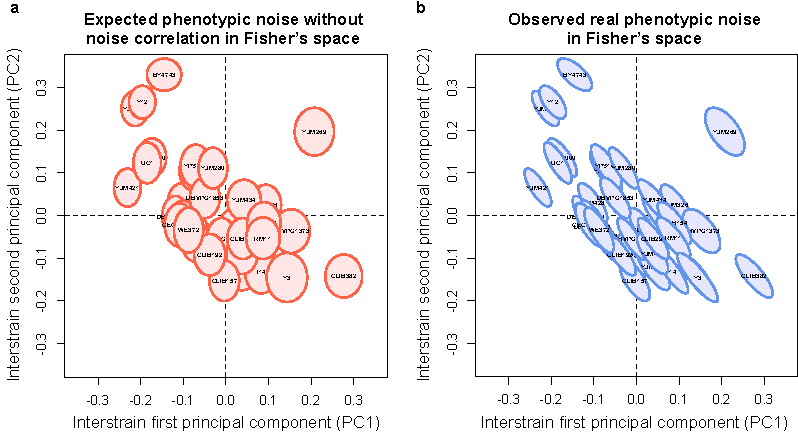
\includegraphics[scale=1]{part1_fig1.pdf}
\end{adjustwidth}
\caption[Yeast intra-strain phenotypic noise is correlated in Fisher's space.]{
\textbf{Yeast intra-strain phenotypic noise is correlated in Fisher's space.}
A singular value decomposition (SVD) is performed on the mean trait values of each of the 37 yeast strains. This space is similar to the phenotypic space used in Fisher's geometric model, where phenotypic characters mutate independently and with the same amplitude (\textit{i.e.} mean phenotype mutations are isotropic in this space). For this reason, we called this space ``Fisher's space''. We then projected single-cell data of each strain in this space. We identified the two Fisher's space axes showing most elevated noise correlation in mean, for all strains: they correspond to the first two components of Fisher's space (PC1 and PC2).
\textbf{a,} Expected phenotypic noise for each strain without noise correlation between Fisher's space axes (each axis representing a linear combination of phenotypic characters). The shape of the phenotypic noise of each strain is symbolized by an ellipse representing the standard deviation of the associated bivariate normal law. Each ellipse is tagged with the corresponding strain name. The size of the ellipses are rescaled by a factor 0.002 to better distinguish them. The coordinates of the center of each ellipse correspond to the real position of the corresponding strain in the Fisher's space (from real data).
\textbf{b,} Real observed phenotypic noise is represented, showing noise correlation between PC1 and PC2 axes, for all the strains.
}
\label{part1:fig1}
\end{figure}

For example on Figure \ref{part1:fig1}a, we show what would be an uncorrelated phenotypic noise for each strain for the two first principal components (PC1 and PC2) of the Fisher's space (the shape of the phenotypic noise of each strain is symbolized by an ellipse representing the standard deviation of the associated bivariate normal law, rescaled by a factor 0.002). On Figure \ref{part1:fig1}b, the real observed phenotypic noise is represented, showing noise correlations for all the strains. The most variable combinations of phenotypic characters (following PC1 and PC2 axes) between strains are also those exhibiting the most correlated intra-strain phenotypic noise. Thus, if one assume that phenotypic differences across strains are adaptive, our result suggests that the phenotypic characters most exposed to directional selection are also the ones with the most correlated phenotypic noise between characters.

Our analysis is described in details in Appendix \ref{part1:AppendixS1}, in Data \ref{part1:DataS1} in Data \ref{part1:DataS2}, and in Script \ref{part1:ScriptS2}.

%%%%%%%%%%%%%%%%%%%%%%%%%

\subsection{Analytical and numerical study of {\sigmaFGM}}

Our analytical and numerical approach followed three steps, as presented in Figure \ref{part1:fig2}. \textbf{(1)} We first studied {\sigmaFGM} in the case of organisms evolving a single phenotypic character, in order to evaluate previous statements \citep{zhang-et-al-2009,eldar-and-elowitz-2010,bodi-et-al-2017} (Fig. \ref{part1:fig2}a). \textbf{(2)} We then studied {\sigmaFGM} for more complex phenotypes when the phenotypic noise is isotropic, to test whether the fitness benefit of phenotypic noise for a single character is maintained for higher phenotypic complexity (Fig. \ref{part1:fig2}b). \textbf{(3)} Finally, we studied analytically and numerically the most general case in {\sigmaFGM}, where noise amplitudes on each character, as well as noise correlations between characters are evolvable, as suggested by our analysis of the phenomic data provided by \cite{yvert-et-al-2013} and by the experimental study by \cite{cressler-et-al-2017} (Fig. \ref{part1:fig2}c).

\begin{figure}[!h]
\begin{adjustwidth}{-0in}{0in}
\centering
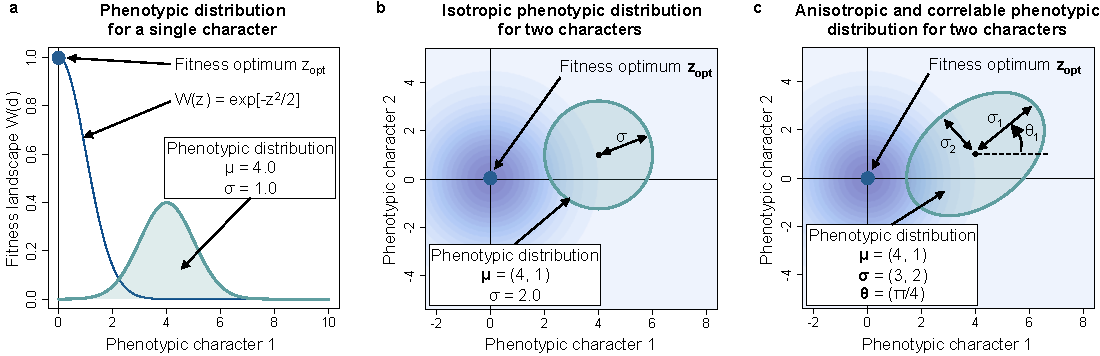
\includegraphics[width=1\linewidth]{part1_fig2.pdf}
\end{adjustwidth}
\caption[Three successive approaches to model phenotypic noise in Fisher's geometric model.]{
\textbf{Three successive approaches to model phenotypic noise in Fisher's geometric model.}
\textbf{a,} Example of an evolvable phenotypic noise on a single phenotypic character ($n=1$). $\mu=4$ and $\sigma=1$ (black box). The phenotypic distribution follows $z \sim \mathcal{N}(\mu,\sigma^2)$ (blue area). The one-dimensional fitness landscape $W(z)=\exp\left[-z^2/2\right]$ is represented in dark blue (dark blue dot: fitness optimum at $z_{opt} = 0$).
\textbf{b,} Example of an evolvable isotropic phenotypic noise on two phenotypic characters ($n=2$). $\boldsymbol{\mu} = (4,1)^T$ and $\sigma=2$ (black box). The standard deviation of the bivariate and isotropic phenotypic distribution is represented by the disc colored in blue. The fitness landscape $W(\boldsymbol{z})$ is represented by a gradient of blue (dark blue dot: fitness optimum at $\boldsymbol{z_{opt}} = (0,0)^T$).
\textbf{c,} Example of an evolvable anisotropic and correlated phenotypic noise on two phenotypic characters ($n=2$).  $\boldsymbol{\mu} = (4,1)^T$, $\boldsymbol{\sigma} = (3,2)^T$ and $\boldsymbol{\theta} = (\pi/4)$ (black box). The standard deviation of the bivariate phenotypic distribution is represented by the blue ellipse colored in blue. The fitness landscape $W(\boldsymbol{z})$ is represented by a gradient of blue (dark blue dot: fitness optimum $\boldsymbol{z_{opt}} = (0,0)^T$).
}
\label{part1:fig2}
\end{figure}

%%%%%%%%%%%%%%%%%%%%%%%%%

\subsubsection{Elevated phenotypic noise is beneficial in directional selection for a single phenotypic character.}

We first studied {\sigmaFGM} in the simple case of the evolution of a single phenotypic character. The phenotypic noise is then reduced to an univariate normal law $\mathcal{N}(\mu,\sigma^2)$, with $\mu$ the single mean trait value and $\sigma$ the standard deviation of the phenotypic noise on this character (Fig. \ref{part1:fig2}a). To understand what would be the selective pressures on $\mu$ and $\sigma$ in the phenotypic space, we analytically studied the sub-population fitness $\overline{W}(\mu,\sigma)$, under the hypothesis of an infinite population (Eq. \ref{eq:integrative_fitness}). The mathematical details of our analytical and numerical approaches are presented in Appendix \ref{part1:AppendixS2} and Appendix \ref{part1:AppendixS3}. Figure \ref{part1:fig3} shows that, if evolvable, phenotypic noise should increase during directional selection, and then decrease when selection becomes stabilizing, as predicted in \cite{eldar-and-elowitz-2010}.
When the population is far from the fitness optimum $z_{opt}$, it is beneficial to increase the phenotypic noise (Fig. \ref{part1:fig3} green area). On the contrary, when the population is near the fitness optimum, or when noise amplitude is too high, it is better to decrease phenotypic noise, as shown in previous studies \citep{mineta-et-al-2015,keren-et-al-2016} (Fig. \ref{part1:fig3} red area).

\begin{figure}[!ht]
\centering
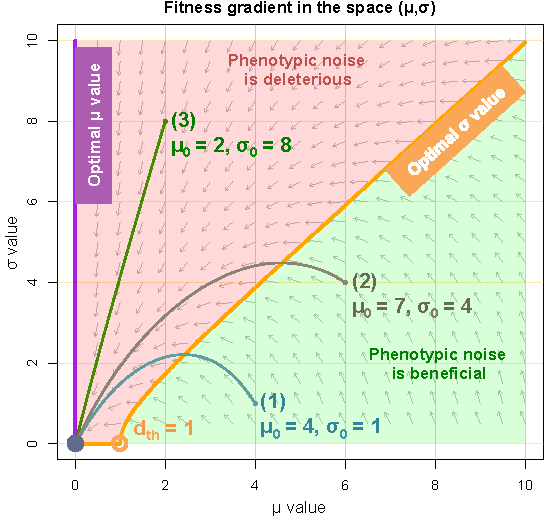
\includegraphics[scale=1]{part1_fig3.pdf}
\caption[Variations of the sub-population fitness $\overline{W}(\mu,\sigma)$ depending on $\mu$ and $\sigma$ values.]{\textbf{Variations of the sub-population fitness $\overline{W}(\mu,\sigma)$ depending on $\mu$ and $\sigma$ values.}
Following the purple curve, the optimal $\mu$ value given a $\sigma$ value. Following the orange curve, the optimal $\sigma$ value given a $\mu$ value. Green area: it is beneficial to increase the phenotypic noise. Red area: it is beneficial to reduce the phenotypic noise. Three trajectories following the fitness gradient are represented \textbf{(1)} in blue (initial values: $\mu_0=4, \sigma_0=1$), \textbf{(2)} in brown (initial values: $\mu_0=6, \sigma_0=4$) and \textbf{(3)} in green (initial values: $\mu_0=2, \sigma_0=8$). Black dot: fitness optimum $z_{opt}$. Orange circle: inflection point $d_{th}=1$ of the fitness landscape $W(z)$. Grey arrows indicate the direction of the fitness gradient, but not its amplitude.
}
\label{part1:fig3}
\end{figure}

Thus, depending on the euclidean distance from the fitness optimum, there exists an optimal value of $\sigma$ giving the highest fitness value, as shown by the orange curve on Figure \ref{part1:fig3}. At the critical distance $d_{th} = 1$ (Fig. \ref{part1:fig3} orange circle, Appendix \ref{part1:AppendixS3}), which corresponds to the inflection point of the fitness function $W(z)$ \citep{zhang-et-al-2009}, phenotypic noise is always deleterious and must be minimized by organisms. However, reducing the euclidean distance from the fitness optimum is always beneficial, whatever the value of $\sigma$, as shown by the purple curve on Figure \ref{part1:fig3}. As exemplified by trajectories \textbf{(1)}, \textbf{(2)} and \textbf{(3)} on Figure \ref{part1:fig3}, a population adapting to the new fitness optimum (Fig. \ref{part1:fig3} dark blue dot) will increase or decrease its phenotypic noise depending on initial conditions. The prediction of \cite{eldar-and-elowitz-2010} corresponds to trajectory \textbf{(1)}, \textit{e.g.}, when a population anciently in stabilizing selection (with reduced phenotypic noise) must adapt to a new environment. Trajectories \textbf{(2)} and \textbf{(3)} could correspond \textit{ e.g.}, to a single stress-related gene, with elevated phenotypic noise at the moment of the environmental shift.

Then, in the case of a population evolving a single phenotypic character, our results confirm the claim that phenotypic noise is beneficial in directional selection, when the population is far from the fitness optimum, and that phenotypic noise is deleterious in stabilizing selection, when the population reaches the fitness optimum \citep{eldar-and-elowitz-2010}. As previously demonstrated by \cite{zhang-et-al-2009}, a condition to the positive selection of phenotypic noise is the existence of a convex fitness landscape. In a recent experimental study on \textit{Saccharomyces cerevisiae}, \cite{keren-et-al-2016} suggest that it could be the case for many traits.

%%%%%%%%%%%%%%%%%%%%%%%%%

\subsubsection{There is a cost of complexity on isotropic phenotypic noise in directional selection}

When organisms evolve a single phenotypic character, {\sigmaFGM} is in accordance with previous results \citep{zhang-et-al-2009,eldar-and-elowitz-2010,bodi-et-al-2017}. However, the fitness effect of phenotypic noise is unclear when the phenotypic complexity increases, since the evolution of phenotypic noise can potentially be impeded by a cost of complexity, as defined by \cite{fisher-1930}. To address this question, we first generalized the one-dimensional case by increasing the number of phenotypic characters, but keeping an isotropic phenotypic noise (similar to a ``global'' phenotypic noise affecting the whole phenotype, \citealt{yvert-et-al-2013}). An isotropic noise is applied to the mean phenotype $\boldsymbol{\mu}$ of an organism, by independently varying each trait value $\mu_i$ with the same amplitude $\sigma$ (Fig. \ref{part1:fig2}b).
In {\sigmaFGM}, this scenario corresponds to constrain the evolution of the covariance matrix $\boldsymbol{\Sigma}$ such that $\boldsymbol{\Sigma} = \sigma^2 \boldsymbol{I_n}$, and to remove noise correlations ($\boldsymbol{\theta} = \boldsymbol{0}$).
We repeated the analysis made for a single phenotypic character, but ranging from a single to 50 characters. The details of our analytical and numerical approaches are presented in Appendix \ref{part1:AppendixS2} and Appendix \ref{part1:AppendixS3}.

The results, presented in Figure \ref{part1:fig4}, show that the advantage of an isotropic phenotypic noise is quickly impeded when the phenotypic complexity increases. First, the euclidean distance $d_{th}$ below which phenotypic noise is deleterious increases with the phenotypic complexity. An analytical resolution shows that $d_{th}$ increases as the square root of the number of phenotypic characters ($d_{th} = \sqrt{n}$, Fig. \ref{part1:fig4}a, and Appendix \ref{part1:AppendixS3}).
Second, the fitness gain brought by an optimal phenotypic noise (Fig. \ref{part1:fig4}a orange and grey curves) quickly vanishes with phenotypic complexity. Indeed, when organisms have more than one phenotypic characters ($n>1$), the beneficial value of phenotypic noise becomes rapidly negligible (Fig. \ref{part1:fig4}b). The maximal fitness gain when phenotypic noise is optimal also rapidly falls down, with \textit{e.g.}, a maximal fitness gain for two characters ($n=2$) representing only $\sim36\%$ of the maximal gain for a single character (Fig. \ref{part1:fig4}b black dots).

These results show that predictions based on the evolution of a single character cannot be generalized as is at the level of the phenotype, when the phenotypic noise is isotropic, as it undergoes a cost of complexity.

\begin{figure}
\centering
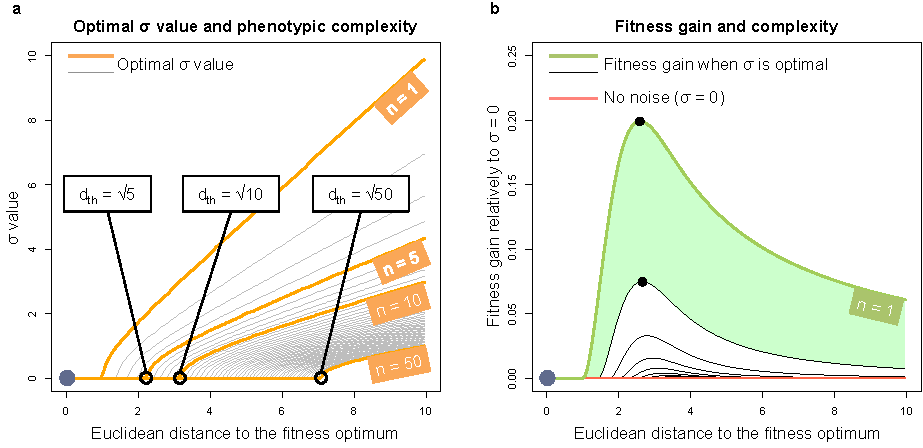
\includegraphics[scale=1]{part1_fig4.pdf}
\caption[Effects of phenotypic complexity on isotropic phenotypic noise fitness gain.]{\textbf{Effects of phenotypic complexity on isotropic phenotypic noise fitness gain.}
\textbf{a,} Variation of the optimal $\sigma$ value, depending on the euclidean distance. $x$ axis: the euclidean distance from the fitness optimum is varied from 0 to 10, for all phenotypic complexities ($d=\lVert \boldsymbol{\mu} \rVert$). $y$ axis: the amplitude $\sigma$ of the phenotypic noise is varied from 0 to 10. Grey curves: optimal $\sigma$ value for each phenotypic complexity. Phenotype complexities $n=1$, $n=5$, $n=10$ and $n=50$ are highlighted in orange. Black circle: the critical euclidean distance $d_{th}$ below which phenotypic noise is always deleterious is equal to $\sqrt{n}$ (exemplified here for $n=5$, $n=10$ and $n=50$).
\textbf{b,} Fitness gain when $\sigma$ is optimal, compared to canonical FGM scenario with no phenotypic noise ($\sigma = 0$). Dark blue dot: fitness optimum. Black curves: fitness gain when isotropic noise is optimal. Phenotypic complexity $n=1$ is highlighted in green. The green area indicates the difference of fitness gain between $n=1$ and $n=2$. Red line: no fitness gain (no phenotypic noise scenario). Black dots: maximal fitness gains when $n=1$ and $n=2$. The maximal fitness gain of isotropic noise when $n=2$ represents $\sim36\%$ of the maximal gain for a single character.
}
\label{part1:fig4}
\end{figure}

%%%%%%%%%%%%%%%%%%%%%%%%%

\subsubsection{Anisotropic and correlated phenotypic noise is beneficial when aligned with the fitness optimum}

Finally, we studied the most general case in {\sigmaFGM}, as described in Methods. Noise amplitude on each character, as well as noise correlations between characters are evolvable (Fig. \ref{part1:fig2}c). As a first step, we analyzed the model in a static situation, with no mutational process (as for previous results), in order to guess what would be the selective pressures on the phenotypic noise.

We show mathematically (Appendix \ref{part1:AppendixS3}) that when the population is far from the fitness optimum, the best configuration (\textit{i.e.}, the one that gives the best fitness advantage) is a flattened, one-dimensional phenotypic noise, with elevated noise in the direction of the fitness optimum and no noise in all other directions. Any other form of phenotypic noise (isotropic or not perfectly aligned with the fitness optimum) gives a lower sub-population fitness $\overline{W}(\boldsymbol{\mu},\boldsymbol{\Sigma})$. This does not mean that a badly aligned phenotypic noise is deleterious for organismal fitness, compared to an organism with no phenotypic noise for example. As shown in Figure \ref{part1:fig4}, even an isotropic noise slightly increases the fitness when the population is far from the fitness optimum. However, as also shown in Figure \ref{part1:fig4}, the best fitness gain is obtained when the phenotypic noise is one-dimensional. Similarly, the best phenotypic noise configuration in $n$ dimensions consists in a dimensionality reduction to fight the cost of complexity on phenotypic noise. A population evolving such a phenotypic noise will recover the benefit of a single character scenario, phenotypic noise conferring a strong fitness advantage to organisms in directional selection (Figs. \ref{part1:fig3} and \ref{part1:fig4}).
The mathematical demonstration of this result is provided in Appendix \ref{part1:AppendixS3}.

%%%%%%%%%%%%%%%%%%%%%%%%%

\subsubsection{Evolvable anisotropic and correlated phenotypic noise compensates for the cost of complexity in directional selection}

To test our mathematical prediction on the evolution of an anisotropic and correlated phenotypic noise (see above), we used a numerical scheme to compute the evolutionary trajectory of an initially maladapted population towards the fitness optimum. To do so, we estimated the evolution of the population distribution $n(\boldsymbol{\mu},\boldsymbol{\sigma},\boldsymbol{\theta})$ through time by simulating the stochastic branching process in finite population associated to the model, as described in Methods.

In directional selection and with a complex phenotype, if organisms are allowed to evolve a correlated phenotypic noise, will they do so? And if yes, what will be the consequence on the evolution speed depending on phenotypic complexity? To address these questions, we measured the convergence time to the fitness optimum of an evolving population in four different scenarios:
\begin{enumerate}
\item[\textbf{(1)}] The mutation sizes $s_\sigma$ and $s_\theta$ of the phenotypic noise parameters $\boldsymbol{\sigma}$ and $\boldsymbol{\theta}$ are lower than for $s_\mu$ ($s_\mu = 0.01, s_\sigma = s_\theta = 0.001$);
\item[\textbf{(2)}] The mutation sizes $s_\sigma$ and $s_\theta$ are equal to the mutation size $s_\mu$ ($s_\mu = s_\sigma = s_\theta = 0.01$);
\item[\textbf{(3)}] The mutation sizes $s_\sigma$ and $s_\theta$ are higher than $s_\mu$ ($s_\mu = 0.01, s_\sigma = s_\theta = 0.1$).
\item[\textbf{(4)}] Organisms have no phenotypic noise, as in canonical FGM ($s_\mu = 0.01, s_\sigma = s_\theta = 0.0$, and $\boldsymbol{\sigma}=\boldsymbol{0}, \boldsymbol{\theta}=\boldsymbol{0}$)
\end{enumerate}

The simulations were computed for a phenotypic complexity ranging from $n=1$ to $n=10$. 100 repetitions have been computed per parameter set. The population was considered to have converged towards the optimum when the mean fitness of the population was higher than 0.9.
All populations were initialized with a very low level of phenotypic noise ($\boldsymbol{\sigma} \sim \boldsymbol{0}$), and no rotation of the covariance matrix $\boldsymbol{\Sigma}$ ($\boldsymbol{\theta} = \boldsymbol{0}$). The initial euclidean distance was $d_{init} = 4.0$ for all the simulations (beyond the critical distance $d_{th} = \sqrt{n}$, see above). To do so, the $\mu_i$ values of the initial mean phenotype $\boldsymbol{\mu}$ were set to $\mu_i = d_{init}/\sqrt{n}$.
To keep the mutation sizes constant whatever the phenotypic complexity, $s_\mu$, $s_\sigma$ and $s_\theta$ were also normalized by $\sqrt{n}$.

To facilitate the analysis of numerical outputs, we used three different measures:
\begin{enumerate}
\item[\textbf{(1)}] The \textit{maximal eigenvalue} indicates the amount of phenotypic noise on the distribution $\mathcal{N}_n(\boldsymbol{\mu},\boldsymbol{\Sigma})$ (Eq. \ref{eq:phenotypic_noise}), and is equal to $\max(\boldsymbol{\sigma}^2)$;
\item[\textbf{(2)}] The \textit{maximal eigenvalue contribution} indicates the contribution of the maximum eigenvalue to the total amount of noise. It is obtained by computing:
\begin{equation}
\dfrac{\max(\boldsymbol{\sigma}^2)}{\sum\limits_{i \in n} \sigma_i^2};
\label{eq:maximum_eigenvalue_contribution}
\end{equation}
\item[\textbf{(3)}] The \textit{maximal eigenvector correlation} is the correlation (dot product) between the eigenvector associated to the maximal eigenvalue, and the direction of the optimum. If the correlation $\approx 1$, the principal axis of the phenotypic distribution is aligned towards the optimum. If the correlation $\approx 0$, the principal axis is orthogonal to the direction of the optimum (by symmetry, we take the absolute value of the dot product).
\end{enumerate}

\begin{figure}[!h]
\begin{adjustwidth}{-0in}{0in}
\centering
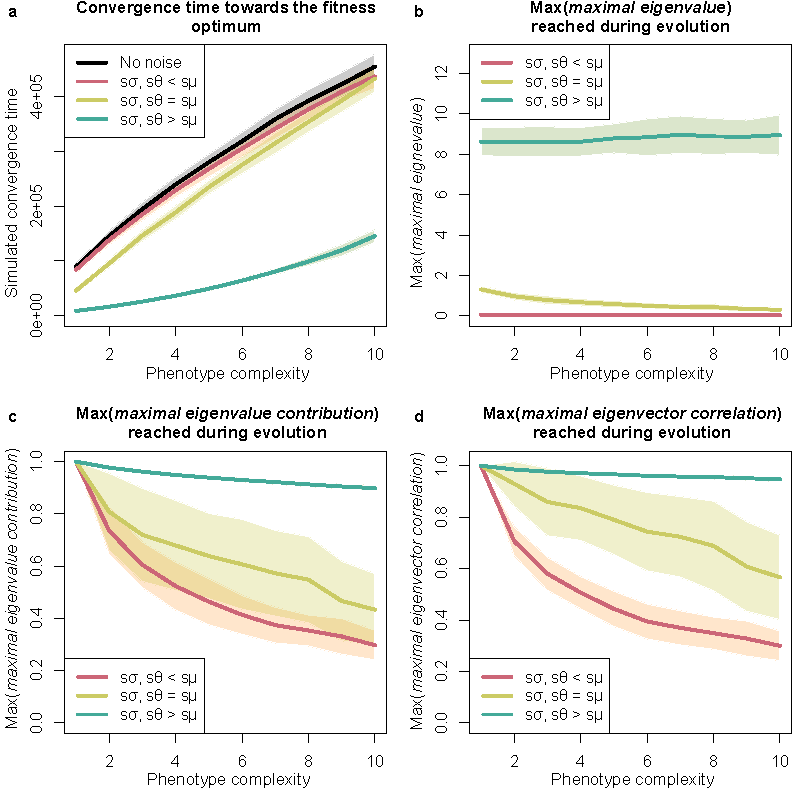
\includegraphics[scale=1]{part1_fig5.pdf}
\end{adjustwidth}
\caption[An evolvable anisotropic and correlated phenotypic noise speeds up evolution.]{\textbf{An evolvable anisotropic and correlated phenotypic noise speeds up evolution.}
\textbf{a,} Convergence time towards the fitness optimum. Four scenarios are evaluated. Black curve: canonical FGM scenario, with no phenotypic noise. Colored curves: evolvable phenotypic noise scenarios. $x$-axis: phenotypic complexity, from $n=1$ to $n=10$. $y$-axis: Convergence time.
\textbf{b, c, d,} Maximum values of \textbf{b,} the \textit{maximum eigenvalue} ($max(\boldsymbol{\sigma})$), \textbf{c,} the \textit{maximum eigenvalue contribution} (Eq. \ref{eq:maximum_eigenvalue_contribution}), and \textbf{d,} the \textit{maximum eigenvalue dot product} (with the direction of the fitness optimum) reached by the population during its evolution towards the fitness optimum, respectively. Four scenarios are evaluated (legends): three with evolvable phenotypic noise, one with no phenotypic noise (canonical FGM scenario). For each scenario, the mean (colored lines) and the standard deviation along the 100 repetitions (shaded areas) are represented. In all cases, the scenario where $s_\sigma, s_\theta >  s_\mu$ is characterized by the evolution of a near perfectly flattened and one-dimensional phenotypic noise, fully aligned with the fitness optimum, as predicted mathematically.
}
\label{part1:fig5}
\end{figure}

For each numerical simulation, both the mean and the variance of these measures have been computed along the 100 repetitions, at each time-step. As shown in Figure \ref{part1:fig5}, an evolvable phenotypic noise speeds up evolution, whatever the phenotypic complexity (Fig. \ref{part1:fig5}a). However, this gain depends on the mutation size of phenotypic noise parameters ($s_\sigma$ and $s_\theta$) relative to the mutation size of the mean trait values ($s_\mu$). If $s_\sigma$ and $s_\theta$ are lower or equal to $s_\mu$, the fitness gain is low (Fig. \ref{part1:fig5}a). If $s_\sigma$ and $s_\theta$ are higher than $s_\mu$, the evolution speed gain is significant, with a convergence time much lower than for canonical FGM scenario (with no phenotypic noise), whatever the phenotypic complexity.
The analysis of the three measures indicates that a cost of complexity exists on the evolution of the phenotypic noise, such that if $s_\sigma, s_\theta \leq s_\mu$, the phenotypic noise does not have the time to evolve towards a one-dimensional shape (with elevated noise in the direction of the fitness optimum, and no noise in all other directions). For each measure (the maximum eigenvalue, its contribution and its dot product), the maximum value reached during a simulation is plotted against the phenotypic complexity, for each of the four scenarios (Figs. \ref{part1:fig5}b,c,d). This maximum value represents the efficacy of evolution in shaping the phenotypic noise in directional selection, knowing that noise increases when the population is far from the fitness optimum, and then decreases when the population reaches the fitness optimum.
A trade-off seems to exist between the convergence time of the mean phenotype $\boldsymbol{\mu}$ and the time needed for evolution to shape the phenotypic noise. On Figure \ref{part1:fig5}b, we see that the maximum eigenvalue does not reach the optimal value $\approx 9.0$ when $s_\sigma, s_\theta \leq s_\mu$. However, when $s_\sigma, s_\theta > s_\mu$, the maximum eigenvalue reaches the optimal value whatever the phenotypic complexity. Indeed, in this situation organisms have time to evolve the most beneficial, flattened form of phenotypic noise.
On Figures \ref{part1:fig5}c and \ref{part1:fig5}d, the maximum eigenvalue contribution and the maximum eigenvalue dot product are strongly lessened with phenotypic complexity when $s_\sigma, s_\theta \leq s_\mu$, while they are almost equal to 1 whatever the phenotypic complexity when $s_\sigma, s_\theta > s_\mu$. In the latter case, the phenotypic noise evolves towards a near perfect flattened form, as predicted previously, hence strongly speeding up adaptation.

%%%%%%%%%%%%%%%%%%%%%%%%% SECTION : DISCUSSION %

\section{Discussion}

The fitness benefit of elevated phenotypic noise in directional selection was foreseen by \cite{eldar-and-elowitz-2010}, who stated that ``\textit{one might expect increased phenotypic noise during periods of adaptation to new environments, followed by reduction in noise when selection becomes stabilizing}''. Based on a mathematical model, \cite{zhang-et-al-2009} also stated that elevated noise would increase the probability to fix beneficial mutations in directional selection, provided that the local fitness landscape is convex. This prediction has been corroborated in a recent experimental study on the evolution of a single gene in \textit{Saccharomyces cerevisiae} \citep{bodi-et-al-2017}. However, these results are based on the evolution of a single phenotypic character, while real phenotypes are much more complex, with multiple characters under selection. We extended Fisher's geometric model \citep{fisher-1930} to account for evolvable phenotypic noise, in order to address the question of how phenotypic noise would evolve in directional selection, when organisms own complex phenotypes. This model, named {\sigmaFGM}, allows for evolvable phenotypic noise amplitudes on each character, but also for evolvable noise correlations between characters, as justified by our analysis of the phenomic data of \cite{yvert-et-al-2013}, and an experimental study by \cite{cressler-et-al-2017}.

First, we studied analytically the case where organisms own a single phenotypic character, and must evolve towards a novel environment. Doing so, we confirmed previous results \citep{zhang-et-al-2009,eldar-and-elowitz-2010,bodi-et-al-2017}: elevated phenotypic noise is beneficial under directional selection, when the population is far from the fitness optimum and experiences a convex fitness landscape. When the population is near the fitness optimum, the phenotypic noise is deleterious and must be minimized, confirming previous statements that phenotypic noise is deleterious under stabilizing selection \citep{mineta-et-al-2015,keren-et-al-2016}.

In 1930, \cite{fisher-1930} hypothesized that organisms evolving towards a fitness optimum experience a cost of complexity, beneficial mutations becoming increasingly harder to fix when the number of phenotypic characters under selection increases. Here, we demonstrated that this cost of complexity also hinders the benefit of an elevated phenotypic noise in directional selection, when noise is isotropic. In this case, when the number of phenotypic characters is higher than one, the beneficial fitness effect of phenotypic noise quickly vanishes. Moreover, the critical distance from the fitness optimum below which the phenotypic noise must be minimized increases as the square root of the number of characters, suggesting that for a constant distance from the fitness optimum, more complex organisms are expected to be less noisy.

Recent studies suggested that phenotypic noise could be considered as a complex phenotypic character, possibly tuned by the genotype-to-phenotype map \citep{yvert-et-al-2013,boukhibar-and-barkoulas-2016}, and correlated \citep{cressler-et-al-2017}. Here, we demonstrated that under directional selection on a convex fitness landscape, the best possible configuration for the phenotypic noise is to evolve towards a flattened, one-dimensional configuration, with elevated noise in the direction of the fitness optimum, and no noise in all other directions. In this case, the evolving population recovers the beneficial value of an elevated phenotypic noise, as for the single phenotypic character scenario. We also demonstrated that in this specific configuration, phenotypic noise increases the probability to fix beneficial mutations and accelerates evolution, whatever the phenotypic complexity, thereby partly compensating for the cost of complexity. To be fully exploitable by evolution, the properties of the phenotypic noise must evolve at a higher speed than the mean phenotype. However, it is not required for the noisy phenotype to be inherited in our model, suggesting that when it is the case \citep{charlebois-et-al-2011}, this constraint could be relaxed.

Our findings are in accordance with recent experimental results. First, \cite{cressler-et-al-2017} demonstrated the existence of correlated phenotypic noise on \textit{Daphnia pulicaria} (a freshwater zooplankton). By measuring three integrated phenotypic characters at the individual level (body growth, number of eggs and longevity) on different populations of genetic variants, they showed that there are no significant genetic correlations between characters, while there is strong evidence for positive non-genetic correlations between characters. Moreover, they showed that increasing phenotypic noise enhances growth rate when non-genetic correlations between characters are positive, in agreement with our prediction on the evolution of phenotypic noise. Second, our analysis of single-cell yeast data provided by \cite{yvert-et-al-2013} revealed that the phenotypic characters showing the strongest noise correlations are also the most variables between strains, suggesting that a correlated phenotypic noise evolved on the phenotypic characters most exposed to directional selection (Appendix \ref{part1:AppendixS1}). Finally, an experimental study by \cite{metzger-et-al-2015} suggested that the expression noise of TDH3 gene may evolve faster than its mean expression, suggesting that it could be the case for phenotypic noise in general, in agreement with our findings.

As a whole, our results show that such non-isotropic phenotypic noise could be exploited by evolution, and suggest further experiments to assess the functional nature of phenotypic noise. In particular, phenotypic noise has been demonstrated to have a role in drug resistance \citep{singh-et-al-2010,charlebois-et-al-2014,charlebois-2015}, cancer cells proliferation \citep{gascoigne-taylor-2008,cohen-et-al-2008,huang-2012,pisco-et-al-2013} as well as in the process of decision-making, seen as an adaptation to a environmental change \citep{richard-et-al-2016}. It could be interesting to initiate new experiments letting biological populations adapt to a novel environment, and acquire phenotypic noise data at the individual level \citep{ohya-et-al-2015}. The long-term evolution experiment (LTEE, \citealt{elena-and-lenski-2003}), where populations of \textit{Escherichia coli} are evolved in a minimum glucose medium since more than 66,000 generations, and regularly frozen to keep track of evolution, would be a good candidate to initiate such an experiment. Moreover, our predictions on the evolution of phenotypic noise in directional selection could be used to predict the future direction of evolution, and to localize the fitness optimum in the phenotypic space. Indeed, tracking the evolution of phenotypic noise experimentally could help biologists understand what are the selective pressures at work on organisms, and to anticipate the next evolution steps.

By extending Fisher's geometric model with evolvable phenotypic noise, we offered general predictions on what would be the evolution of phenotypic noise in directional selection, and its consequences on the fate of asexual populations experiencing directional selection.
Our demonstrations rely on the assumption that the phenotypic noise and the fitness landscape are Gaussian-shaped, as it is historically the case in Fisher's geometric model. If the phenotypic noise is not Gaussian, other particular cases could appear, even if locally there is always a benefit to be noisy in directions where the fitness is convex. By relaxing our hypotheses, other interesting questions could be tackled, for example the case where the fitness landscape is multimodal or not static, the case of a degenerated noise (\textit{e.g.}, where some directions in the phenotypic space are forbidden), or whether the case of a multiplicative noise. By deciphering the conditions in which phenotypic noise evolves towards specific patterns, our results may contribute to the growing field of predictive biology.

\newpage

%%%%%%%%%%%%%%%%%%%%%%%%% SECTION : SUPPORTING INFORMATION %

\section{Supporting Information}

%%%%%%%%%%%%%%%%%%%%%%%%%%%

\subsection{Figure S1. An example of the temporal dynamics in {\sigmaFGM}.}
\label{part1:FigureS1}

\begin{figurehere}
\begin{adjustwidth}{-0in}{0in}
\centering
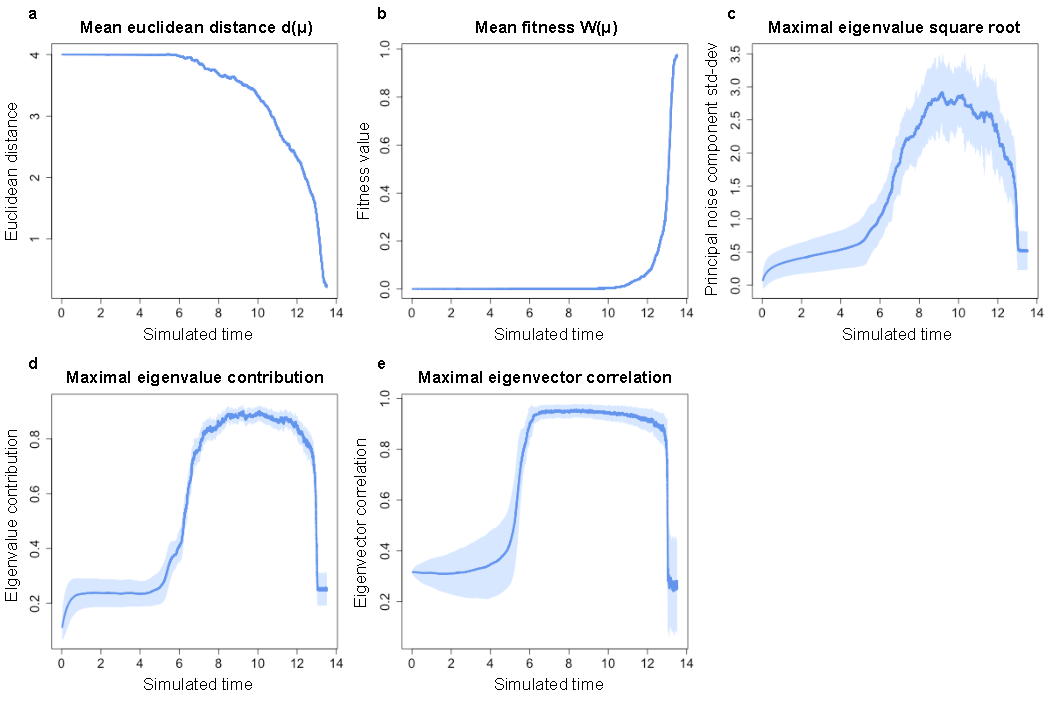
\includegraphics[width=1\linewidth]{part1_figS1.pdf}
\end{adjustwidth}
\caption[An example of the temporal dynamics in {\sigmaFGM}.]{
\textbf{An example of the temporal dynamics in {\sigmaFGM}.}
A simulation in $n=10$ dimensions is initialized with 10,000 organisms having the same triplet $(\boldsymbol{\mu}_0, \boldsymbol{\sigma}_0, \boldsymbol{\theta}_0)$, with $\boldsymbol{\mu}_0 = \{4.0/\sqrt{n}\}^T$, $\boldsymbol{\sigma}_0=\boldsymbol{0}$, and $\boldsymbol{\theta}_0=\boldsymbol{0}$. The initial population is then localized on the hyper-sphere of radius 4.0, none of the phenotypic characters being aligned with the fitness optimum $z_{opt}$, and thus requiring to be adapted. $s_\mu=0.01$, and $s_\sigma=s_\theta=0.1$. The simulation stopped when the population mean of the mean fitness $\langle W(\boldsymbol{\mu}) \rangle$ reached 0.9.
\textbf{a,} The population mean of the mean euclidean distance $\langle d(\boldsymbol{\mu}) \rangle$.
\textbf{b,} The population mean of the mean fitness $\langle W(\boldsymbol{\mu}) \rangle$.
\textbf{c,} The population mean of the maximal eigenvalue.
\textbf{d,} The population mean of the maximal eigenvalue contribution.
\textbf{e,} The population mean of the maximal eigenvector correlation with the direction of the fitness optimum.
The standard deviation of each variable is represented by a shaded blue area.
}
\label{figS1}
\end{figurehere}

\newpage

%%%%%%%%%%%%%%%%%%%%%%%%%%%

\subsection{Appendix S1. Various wild-types of yeast exhibit correlated phenotypic noise.}
\label{part1:AppendixS1}


In this appendix, we present the results of our analysis on the experimental single-cell data provided by \cite{yvert-et-al-2013}. We assume that the reader is aware of the basic definitions and equations provided in the main manuscript.

\cite{yvert-et-al-2013} used automated image analysis to describe yeast phenotypic diversity at a single-cell resolution (known as phenomics, \citealt{ohya-et-al-2015}). They monitored $n=125$ phenotypic characters on isogenic populations of $m=37$ different strains of yeast, living in natural or laboratory conditions. For each strain, they measured 5 replicates of approximately 200 cells each ($\sim$1000 cells per strain). They demonstrated that phenotypic noise significantly differs between strains, supporting ``\textit{the possibility that, if noise is adaptive, microevolution may tune it in the wild}'' \citep{yvert-et-al-2013}.

We used the raw datasets published by the authors to measure intra-strain (\textit{i.e.} isogenic) noise correlations between characters. The goal of our study is to test the existence of correlated phenotypic noise in natural strains of yeast. The datasets provided by \cite{yvert-et-al-2013} are structured as following: for each strain of yeast, a set of files is provided in a dedicated folder (a dataset per replicate). For each replicate, the list of single-cell measures is dispatched in three different files in \texttt{xls} format. Each cell is identified by a unique tag per image and the tag of the captured image. Each time a measure failed (on one character, or on the entire cell), the corresponding element (or line) in the table was filled with value $-1$.
Several characters are redundant (for example the volume and the size of the nucleus), and strongly correlated. Moreover, each trait value is provided with specific units (\textit{e.g.}, number of pixels, volume or angle units), such that some normalization is necessary.
The code associated to this analysis is freely available in Script \ref{part1:ScriptS2}. One can run again the whole analysis by following instructions provided in the README file. The raw dataset is freely provided by \cite{yvert-et-al-2013}.

The purpose of the analysis is to determine whether intra-strain variability presents correlations between characters \textit{once inter-strain correlations  between characters have been removed}. 

Let us first process inter-strain variability. The idea is to find a phenotypic space in which there is as little character-specific variability and correlation as possible. Here we have 37 isogenic strains, hence 37 genotypes. We define the ``phenotype'' of a strain/genotype as the vector of mean trait values, computed over all cells from this strain/genotype. We then define the ``centered phenotype" of a strain/genotype by removing the grand mean of each character. The singular value decomposition of the 37x125 matrix of centered strain phenotypes will give us a set of orthonormal linear combinations of characters. By construction, when the centered strain phenotypes are expressed according to these new characters, they lose all their pairwise correlations, implying that the variance-covariance matrix is diagonal for those new characters. Moreover, we normalize the variance of each new strain phenotype to one\footnote{Which is why our analysis is not exactly a PCA: We drop the singular values that are usually left in the PCA.}, such that the 37 new strain phenotypes are isotropically distributed.

This new base is the closest analogy we could think of to the phenotypic space in the classical version of Fisher's geometric model. Fisher's phenotypic space is orthogonal and normalized, and mutations on the genotype cause phenotypic traits to vary independently and with the same amplitude, according to an isotropic mutational distribution.

The second step is to project intra-strain single-cell data in Fisher's space, and to analyze the possible remaining correlations of intra-strain phenotypic variability in this space.

Figure \ref{part1:appendixS1:fig1} shows the detailed steps of our analysis, as described  below. First, we converted each \texttt{xls} file into \texttt{csv} format, and we merged the three files of each replicate to obtain a single dataset $\boldsymbol{M_{0,s,r}}$ ($s \in \{1,...,37\}$, $r \in \{1,...,5\}$) per replicate, and we removed useless information (such as cell identifiers, coordinates on the image, and so on) (Fig. \ref{part1:appendixS1:fig1}.1).
Then we merged the 5 replicates of each strain (Fig. \ref{part1:appendixS1:fig1}.2) to compute the matrix $\boldsymbol{M_0}$ of the mean phenotypic characters per strain (Fig. \ref{part1:appendixS1:fig1}.3).
Each column ${\boldsymbol{M_0}}_j$ of $\boldsymbol{M_0}$ was centered and normalized to obtain the matrix $\boldsymbol{M}$ (Fig. \ref{part1:appendixS1:fig1}.4):
\begin{equation}
{\boldsymbol{M}}_j = \dfrac{{\boldsymbol{M_0}}_j-\mathrm{mean}({\boldsymbol{M_0}}_j)}{\mathrm{stdev}({\boldsymbol{M_0}}_j)}.
\end{equation}
We also standardized each replicate to obtain $37\times5$ matrices $M_{s,r}, s \in \{1,...,37\}, r \in \{1,...,5\}$ (Fig. \ref{part1:appendixS1:fig1}.6). For each column ${\boldsymbol{M_{0,s,r}}}_j$ of $\boldsymbol{M_{0,s,r}}$:
\begin{equation}
{\boldsymbol{M_{s,r}}}_j = \dfrac{{\boldsymbol{M_{0,s,r}}}_j-\mathrm{mean}({\boldsymbol{M_{0,s,r}}}_j)}{\mathrm{stdev}({\boldsymbol{M_{0,s,r}}}_j)}.
\end{equation}
To find Fisher's space, we computed a SVD from $\boldsymbol{M}$ (see details below, and Fig. \ref{part1:appendixS1:fig1}.5).
For each standardized replicate dataset $\boldsymbol{M_{s,r}}$, many trait values are missing, and are replaced by $-1$ values, making impossible some mathematical operations. For this reason, a next step was to estimate the missing values: we used a simple conservative method, as described below (Fig. \ref{part1:appendixS1:fig1}.7). Finally, each replicate dataset was projected in Fisher's space (Fig. \ref{part1:appendixS1:fig1}.8). The inter-replicate variability was evaluated to ensure that experimental variability is low enough (Fig. \ref{part1:appendixS1:fig1}.9), and intra-strain phenotypic noise correlations were analyzed (Fig. \ref{part1:appendixS1:fig1}.10).

We describe below the steps requiring details.

%%%%%%%%%%%%%%%%%
%%%%%%%%%%%%%%%%%

\section*{Estimation of missing values}
To estimate missing values, we first computed the cell-to-cell Pearson correlation matrix $\boldsymbol{C}$ associated to each replicate, based on available data.
Knowing there are $m' \sim 200$ cells and $n=125$ phenotypic characters in each replicate, we defined a cell by a vector $\boldsymbol{X_i} \in \mathbb{R}^{125}$, with $i \in \{1,...,m'\}$.

Each missing value $x_{i,j}$ of $\boldsymbol{X_i}$ (with $j \in \{1,...,n\}$) was recovered by computing:
\begin{equation}
x_{i,j} = \bar{\boldsymbol{X_i}}+ \dfrac{\sum\limits_{k=1}^{m'} (x_{k,j}-\bar{\boldsymbol{X_k}})c_{i,k}}{\sum\limits_{k=1}^{m'} |c_{i,k}|}
\end{equation}
with $c_{i,k}$ element of $\boldsymbol{C}$. This simple method is conservative, meaning that noise amplitudes tend to be reduced through this estimation method.
Moreover, we removed all cells $X_i$ that contained only $-1$ values.

%%%%%%%%%%%%%%%%%
%%%%%%%%%%%%%%%%%

\section*{Singular value decomposition}
Let us consider the matrix $\boldsymbol{M}$ of dimension $m \times n$ that contains the standardized mean phenotypic trait values of each strain, where $m$ is the number of strains ($m=37$), and $n$ is the number of characters ($n=125$).
$\boldsymbol{M}$ can be decomposed into a $m \times m$ unitary matrix $\boldsymbol{U}$, a $m \times n$ positive and diagonal matrix $\boldsymbol{\Sigma}$, and a $n \times n$ unitary matrix $\boldsymbol{V}$ such that:
\begin{equation}
\boldsymbol{M} = \boldsymbol{U} \boldsymbol{\Sigma} \boldsymbol{V}^*
\label{eq:part1:sigmaFGM:SVD}
\end{equation}
with $\boldsymbol{V}^*$ being the conjugate transpose of $\boldsymbol{V}$.

The diagonal entries of $\boldsymbol{\Sigma}$ are the singular values $\boldsymbol{\sigma} \in \mathbb{R}^m$ of $\boldsymbol{M}$. $\boldsymbol{V}$ contains the right-singular vectors of $\boldsymbol{M}$, defining the base where $m$ linear combinations of phenotypic characters are separated and orthonormal. These linear combinations give 37 new phenotypic characters, whose means vary independently and have been normalized to the same amplitude. In the following, we will call the space generated by the base $\boldsymbol{V}$ the ``Fisher's space''.

As shown on Figure \ref{part1:appendixS1:fig2}, looking at the vector $\boldsymbol{\sigma}$ reveals that only the first 8 singular values carry significant variability between mean phenotypic characters (a method to keep significant singular values consists in removing all values after the shoulder point in Fig. \ref{part1:appendixS1:fig2}). We thus truncated matrices $\boldsymbol{V}$ and $\boldsymbol{\Sigma}$ to only keep the most significant singular values and singular vectors.
To this aim, we defined the matrix $\boldsymbol{V_{cut}}$ of size $n \times 8$ containing the 8 first singular vectors of $\boldsymbol{V}$, and the matrix $\boldsymbol{\Sigma_{cut}}$ of size $8 \times 8$ containing the first 8 singular values $\boldsymbol{\sigma_{cut}}$ such that $\boldsymbol{\Sigma_{cut}} = \mathrm{diag}(\boldsymbol{\sigma_{cut}})$.

%%%%%%%%%%%%%%%%%
%%%%%%%%%%%%%%%%%

\section*{Intra-strain data projection in Fisher's space}
Since the singular value decomposition has been computed on $\boldsymbol{M}$, and the most significant singular values and vectors have been isolated, we can use the base $\boldsymbol{V_{cut}}$ and the diagonal matrix $\boldsymbol{\Sigma_{cut}}$ to project each replicate data in Fisher's space. Let us define the $m' \times n$ matrix $\boldsymbol{M_{s,r}}$ which contains the single-cell data of the replicate $r \in \{1,...,5\}$ of the strain $s \in \{1,...,37\}$. $m'$ is the number of cells ($m' \sim 200$), and $n$ is the number of characters ($n=125$). The projection of $\boldsymbol{M_{s,r}}$ in Fisher's space is computed as following:
\begin{equation}
\boldsymbol{M'_{s,r}} = \boldsymbol{M_{s,r}} \boldsymbol{V_{cut}} \boldsymbol{\Sigma_{cut}}^{-1}
\label{eq:part1:sigmaFGM:projection}
\end{equation}
with $\boldsymbol{\Sigma_{cut}}^{-1} = \mathrm{diag}(1/\boldsymbol{\sigma_{cut}})$ a diagonal matrix where the diagonal entries are the reciprocal of the first 8 singular values. $\boldsymbol{M'_{s,r}}$ represents the single-cell data of the replicate $r$ of the strain $s$, projected in Fisher's space.

%%%%%%%%%%%%%%%%%
%%%%%%%%%%%%%%%%%

\section*{Results}

%%%%%%%%%%%%%%%%%

\subsection*{Inter-replicate variability does not impair phenotypic noise analysis.}

A first step in our analysis of intra-strain phenotypic noise is to check the absence of significant experimental variability between replicates. To this aim, we compared the structure of each replicate. For each replicate dataset $\boldsymbol{M_{s,r}}$ (with $r \in \{1,...,5\}$ and $s \in \{1,...,37\}$), we computed the vectors $\boldsymbol{\mu_{s,r}}$ and $\boldsymbol{\sigma_{s,r}}$ containing respectively the means and the standard deviations by character of $\boldsymbol{M_{s,r}}$. As shown in Figures \ref{part1:appendixS1:fig3} and \ref{part1:appendixS1:fig4}, replicates do not vary significantly from each other (each plot represents a strain, with one color per replicate). We also computed and plotted the correlation matrix of each replicate (5 matrices per strain) to check that experimental variability does not affect noise correlation structure. Noise correlations appeared to not strongly vary between replicates of each strain. The 37 figures corresponding to the 5 correlation matrices of each strain are provided in Data \ref{part1:DataS1}.

As a conclusion, we didn't notice impairing experimental variability between replicates. For this reason, we decided to merge replicates in a single dataset to facilitate further analyses.

%%%%%%%%%%%%%%%%%

\subsection*{Phenotypic noise correlation matrices for each strain.}

As described previously, experimental variability between replicates is low enough to allow us to merge replicates in a single dataset $\boldsymbol{M'_i}$, with $i \in \{1,...,37\}$.
First, in order to identify possible phenotypic noise correlations in Fisher's space, we computed the correlation matrix of $\boldsymbol{M'_i}\ \forall\ i$, and performed a Pearson correlation test on each off-diagonal pair of variables, with $\alpha = 0.05$. A Bonferroni correction of $k=28$ ($k=8*7/2$) was also applied on each test.
Then, we focused on the phenotypic characters exhibiting elevated noise correlations, as shown below.

Correlation matrices demonstrated that all the natural strains of yeast studied in \cite{yvert-et-al-2013} exhibit correlated phenotypic noise in Fisher's space (defined before as the space where inter-strain mean phenotypic characters are uncorrelated and of the same amplitude). For each strain, we found significant noise correlations, despite the Bonferroni correction ($k=28$).
For each correlation matrix, we generated a figure showing the correlations and the results of the Pearson correlation test. For each pair of characters, the strength of the correlation is symbolized by the size of the corresponding circle. A blue color indicates a positive correlation, and a red color a negative correlation. When the Pearson correlation test is negative, the corresponding circle is marked with a cross. The 37 figures corresponding to the correlation matrix of each strain are provided in \ref{part1:DataS2}.

%%%%%%%%%%%%%%%%%

\subsection*{Phenotypic characters with the highest noise correlation are also the most variable between strains.}

For each strain, we also identified the two axes of the phenotypic space showing the highest phenotypic noise correlation. As shown in Figure \ref{part1:appendixS1:fig5}, in a majority of strains, these two axes correspond to the first two axes of Fisher's space. These axes correspond to the most variable inter-strain mean phenotypic characters.
On Figure \ref{part1:appendixS1:fig6}a, we show what would be an uncorrelated phenotypic noise for each strain for the two first principal components (PC1 and PC2) of the Fisher's space (the shape of the phenotypic noise of each strain is symbolized by an ellipse representing the standard deviation of the associated bivariate normal law, rescaled by a factor 0.002). On Figure \ref{part1:appendixS1:fig6}b, the real observed phenotypic noise is represented, showing noise correlations for all the strains.

One must remember that PC1 and PC2 axes are a combination of phenotypic characters. The most variable combinations of phenotypic characters between strains are also the ones exhibiting the most correlated intra-strain phenotypic noise. Thus, if one assume that phenotypic differences across strains are adaptive, this result suggests that the phenotypic characters most exposed to directional selection are also the ones with the most correlated phenotypic noise between characters.

%%%%%%%%%%%%%%%%%%%%%%%%%%%%

\newpage

\begin{figurehere}
\begin{adjustwidth}{-0in}{0in}
\centering
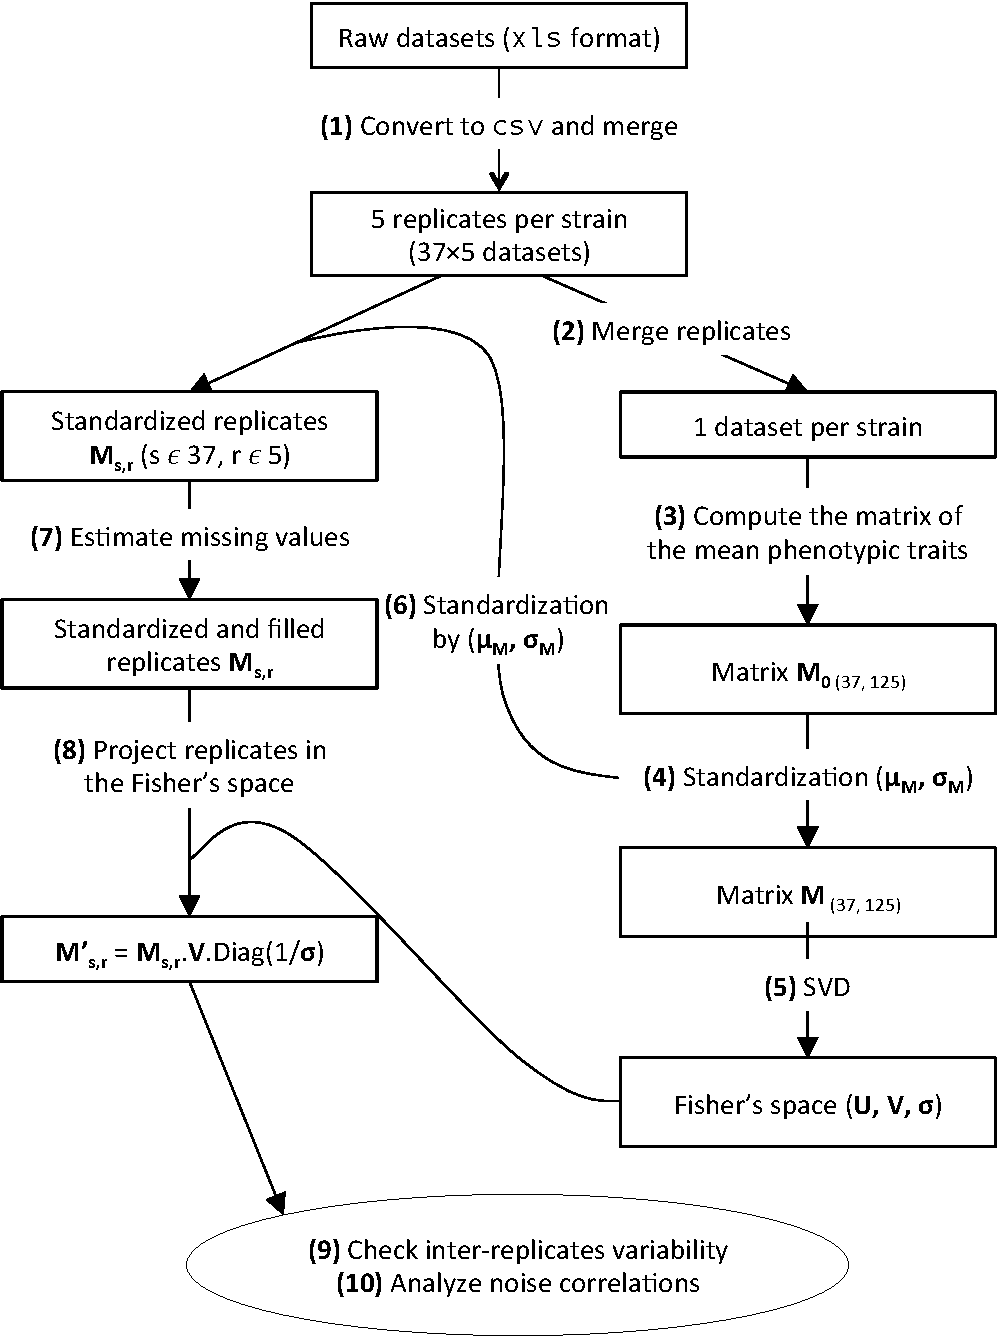
\includegraphics[scale=0.75]{part1_appendixS1_fig1.pdf}
\end{adjustwidth}
\caption[Step-by-step protocol used to analyze single-cell data.]{
\textbf{Step-by-step protocol used to analyze single-cell data.}
\textbf{(1)} Each \texttt{xls} file is converted into \texttt{csv} format, the three files related to each replicate being merged to obtain a single dataset $\boldsymbol{M_{0,s,r}}$ ($s \in \{1,...,m=37\}$, $r \in \{1,...,5\}$) per replicate.
\textbf{(2)} The 5 replicates of each strain are merged to obtain a single dataset per strain.
\textbf{(3)} The matrix $\boldsymbol{M_0}$ of the mean phenotypic trait values per strain is computed.
\textbf{(4,6)} Datasets are standardized according to the mean vector $\boldsymbol{\mu_M} \in \mathbb{R}^{125}$ and the standard deviation vector $\boldsymbol{\sigma_M} \in \mathbb{R}^{125}$ of $\boldsymbol{M_0}$.
\textbf{(5)} A singular values decomposition (SVD) is computed from standardized inter-strain dataset $\boldsymbol{M}$ (see above for the details of the SVD).
\textbf{(7)} Replicate missing values are estimated (see above).
\textbf{(8)} Each replicate dataset is projected into Fisher's space.
\textbf{(9)} Inter-replicate variability is evaluated to ensure that experimental variability is low enough.
\textbf{(10)} Intra-strain phenotypic noise correlations are analyzed.
}
\label{part1:appendixS1:fig1}
\end{figurehere}

%%%%%%%%%%%%%%%%%%%%%%%%%%%%

\newpage

\begin{figurehere}
\begin{adjustwidth}{-0in}{0in}
\centering
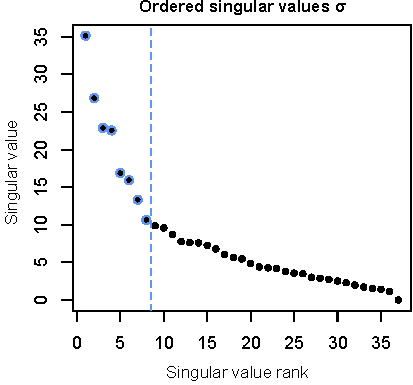
\includegraphics[scale=1.5]{part1_appendixS1_fig2.pdf}
\end{adjustwidth}
\caption[Ordered singular values contained in $\boldsymbol{\sigma}$.]{
\textbf{Ordered singular values contained in $\boldsymbol{\sigma}$.}
A simple empirical method to keep only significant variations is to isolate all the singular values located before the shoulder point in the ordered plot (as shown by a blue dashed line). Here, we kept the first 8 singular values.
}
\label{part1:appendixS1:fig2}
\end{figurehere}

%%%%%%%%%%%%%%%%%%%%%%%%%%%%

\newpage

\begin{figurehere}
\begin{adjustwidth}{-0in}{0in}
\centering
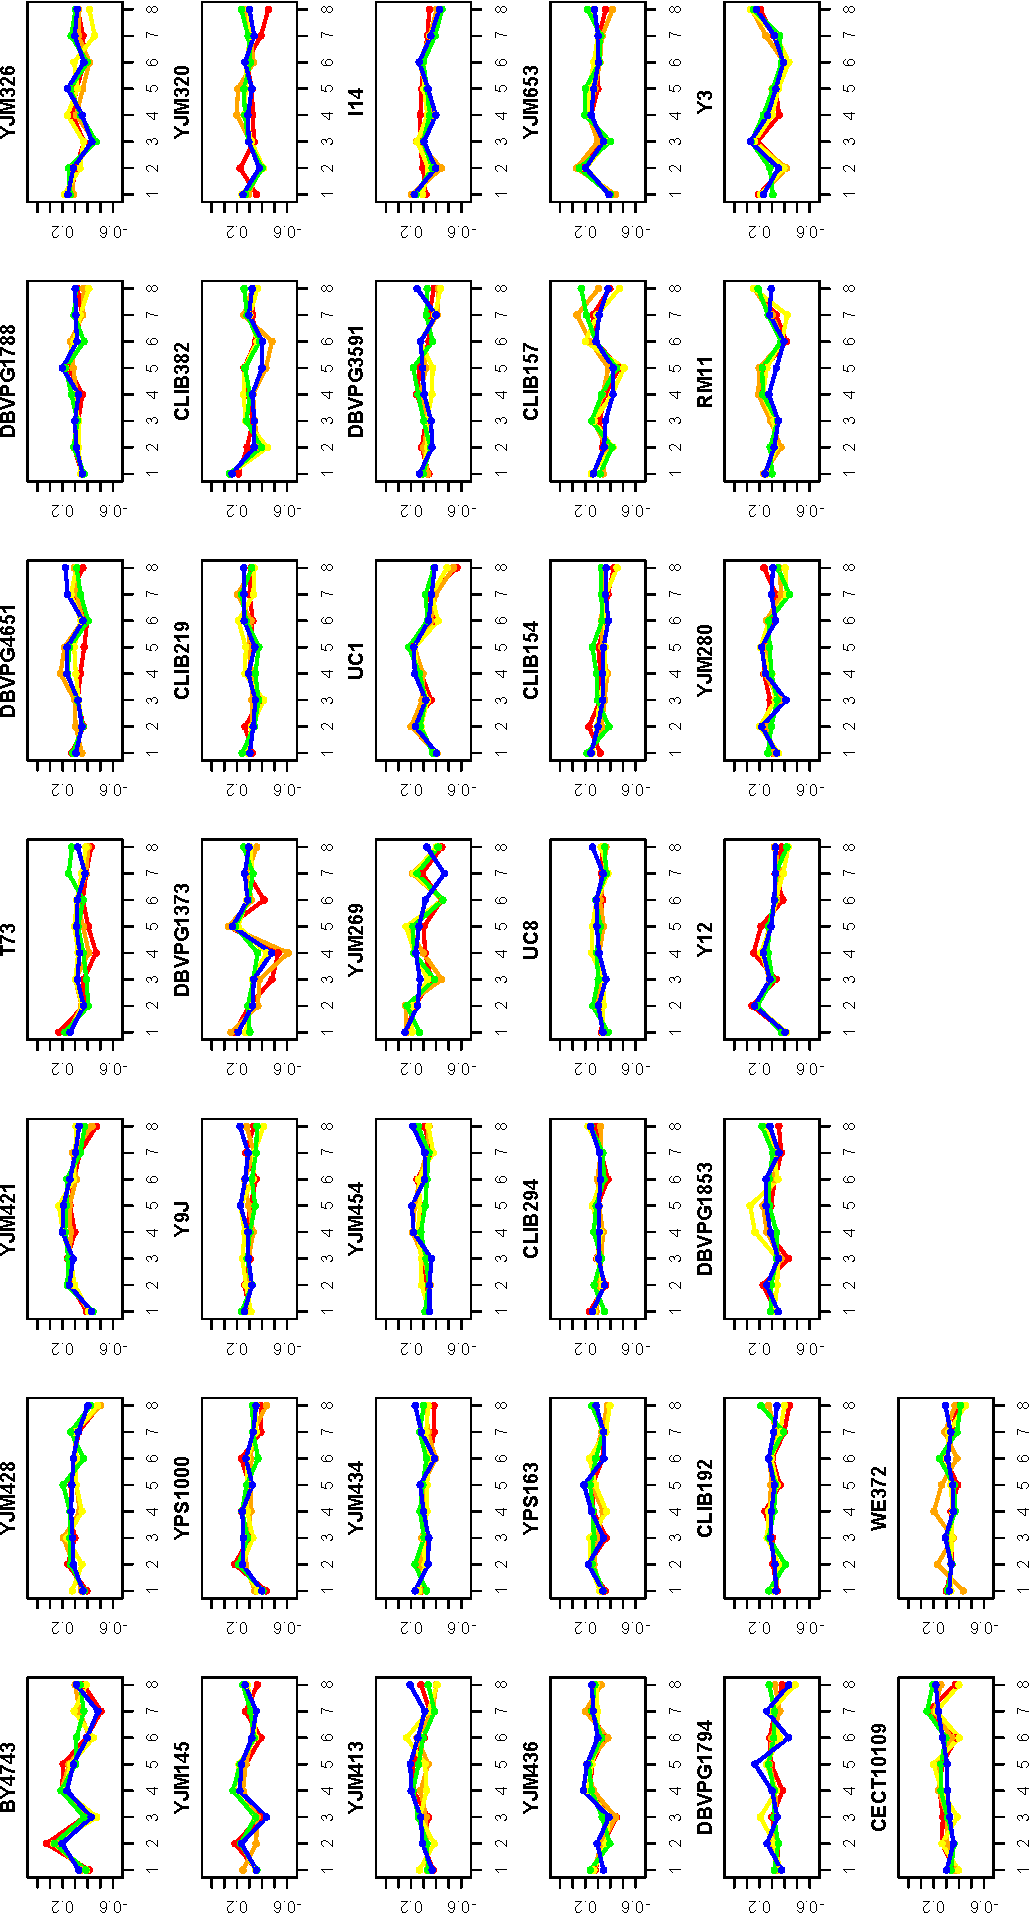
\includegraphics[scale=0.65]{part1_appendixS1_fig3.pdf}
\end{adjustwidth}
\caption[Mean phenotypic trait values per replicate per strain.]{
\textbf{Mean phenotypic trait values per replicate per strain.}
For each replicate of each strain, the mean phenotypic trait values are plotted (one color per replicate on each plot, one plot per strain).
}
\label{part1:appendixS1:fig3}
\end{figurehere}

%%%%%%%%%%%%%%%%%%%%%%%%%%%%

\newpage

\begin{figurehere}
\begin{adjustwidth}{-0in}{0in}
\centering
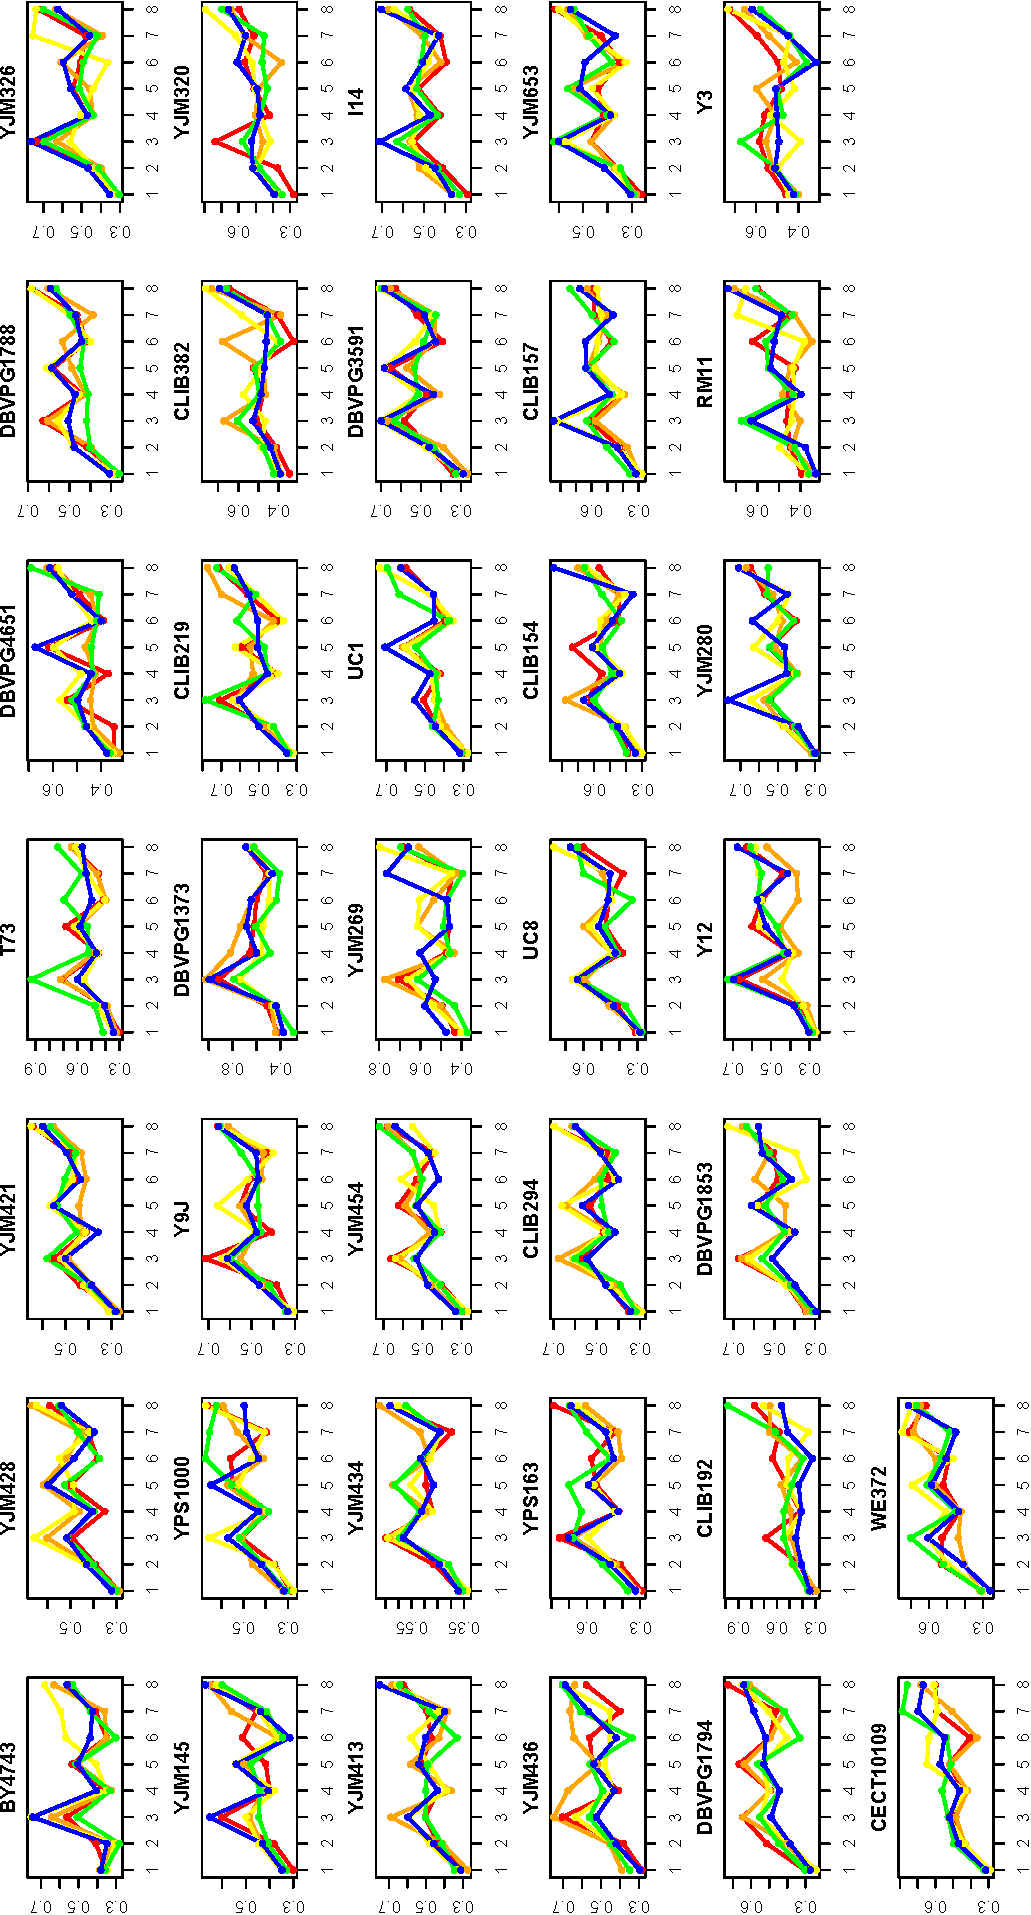
\includegraphics[scale=0.65]{part1_appendixS1_fig4.pdf}
\end{adjustwidth}
\caption[Standard deviation of each phenotypic character per replicate per strain.]{
\textbf{Standard deviation of each phenotypic character per replicate per strain.}
For each replicate of each strain, the standard deviation of each phenotypic character is plotted (one color per replicate on each plot, one plot per strain).
}
\label{part1:appendixS1:fig4}
\end{figurehere}

%%%%%%%%%%%%%%%%%%%%%%%%%%%%

\newpage

\begin{figurehere}
\begin{adjustwidth}{-0in}{0in}
\centering
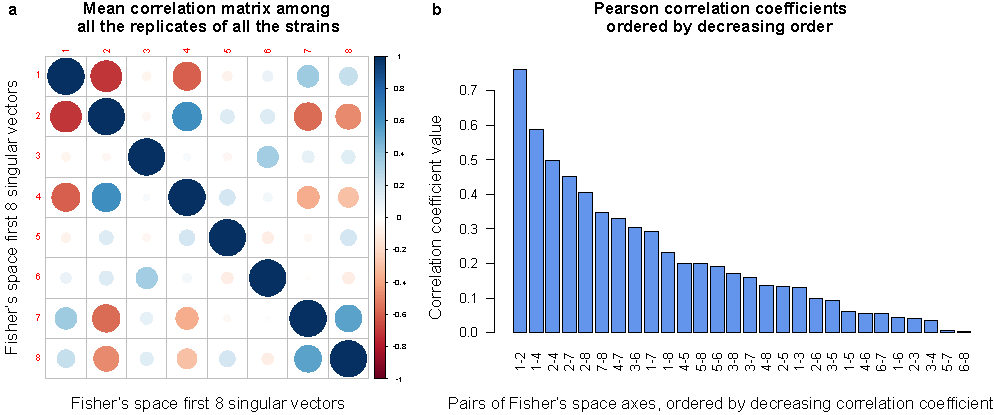
\includegraphics[scale=0.9]{part1_appendixS1_fig5.pdf}
\end{adjustwidth}
\caption[Mean phenotypic noise correlations in the Fisher's space.]{
\textbf{Mean phenotypic noise correlations in the Fisher's space.}
\textbf{a,} The mean correlation matrix across all the replicates of all the strains has been computed and plotted here. For each pair of characters, the strength of the correlation is symbolized by the size of the corresponding circle. A blue color indicates a positive correlation, and a red color a negative correlation.
\textbf{b,} All off-diagonal pairwise correlations between the first 8 axes of Fisher's space are sorted by decreasing order. The most correlated axes in mean are axes 1 and 2 (called PC1 and PC2).
}
\label{part1:appendixS1:fig5}
\end{figurehere}

%%%%%%%%%%%%%%%%%%%%%%%%%%%%

\newpage

\begin{figurehere}
\begin{adjustwidth}{-0in}{0in}
\centering
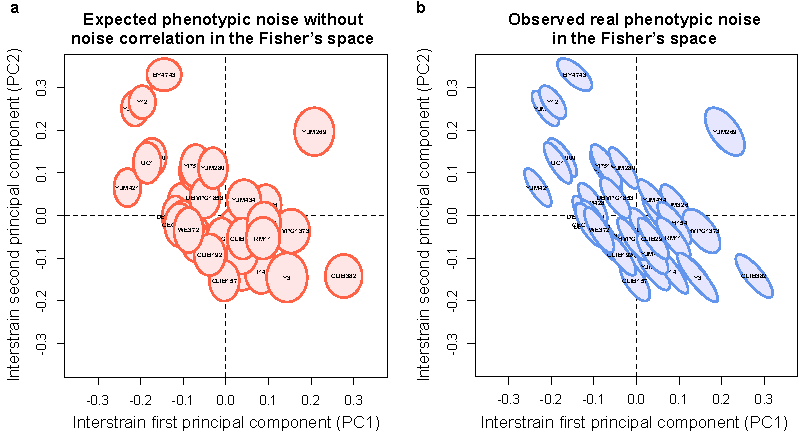
\includegraphics[scale=1]{part1_appendixS1_fig6.pdf}
\end{adjustwidth}
\caption[Yeast intra-strain phenotypic noise is correlated in the Fisher's space.]{
\textbf{Yeast intra-strain phenotypic noise is correlated in the Fisher's space.}
A singular value decomposition (SVD) was performed on the mean trait values of each of the 37 yeast strains. This space is similar to the phenotypic space used in Fisher's geometric model, where phenotypic characters mutate independently and with the same amplitude (\textit{i.e.} mean phenotype mutations are isotropic in this space). For this reason, we called this space ``Fisher's space''. We then projected single-cell data of each strain in this space. We identified the two axes showing the highest noise correlation in mean, for all strains: they correspond to the two first components of Fisher's space (PC1 and PC2).
\textbf{a,} Expected phenotypic noise for each strain without noise correlation between Fisher's space axes (each axis representing a linear combination of phenotypic characters). The shape of the phenotypic noise of each strain is symbolized by an ellipse representing the standard deviation of the associated bivariate normal law. Each ellipse is tagged with the corresponding strain name. The size of the ellipses are rescaled by a factor 0.002 to better distinguish them. The coordinates of the center of each ellipse correspond to the real position of the corresponding strain in Fisher's space (from real data).
\textbf{b,} Real observed phenotypic noise is represented, showing noise correlation between PC1 and PC2 axes, for all the strains.
}
\label{part1:appendixS1:fig6}
\end{figurehere}



\newpage

%%%%%%%%%%%%%%%%%%%%%%%%%%%

\subsection{Appendix S2. A numerical solver for {\sigmaFGM}.}
\label{part1:AppendixS2}


In this appendix, we present in more details the numerical solver of {\sigmaFGM}. We assume that the reader is aware of the basic definitions and equations provided in the main manuscript.

To estimate the evolution of the population distribution $n(\boldsymbol{\mu}, \boldsymbol{\sigma}, \boldsymbol{\theta})$ through time, we simulated the stochastic branching process associated to {\sigmaFGM} equations (as discussed in Methods). Once initial conditions are defined (Table \ref{part1:appendixS2:table1}), the evolutionary trajectory of $n(\boldsymbol{\mu}, \boldsymbol{\sigma}, \boldsymbol{\theta})$ is simulated through time using Algorithm \ref{part1:appendixS2:algorithm1}, which is similar to a time-adaptive tau-leaping algorithm \citep{gillespie-2007}.

%%%%%%%%%%%%%%%%%
%%%%%%%%%%%%%%%%%

\section*{Parameters of the numerical solver}

\begin{table}[!ht]
\begin{adjustwidth}{-0in}{0in}
\centering
\caption{List of parameters of the numerical solver for {\sigmaFGM}.}
\begin{tabular}{|l|c|c|}
\hline
Variable & Symbol & Domain\\
\hline
Number of particles & N & $[1, +\infty]$\\
Number of phenotypic characters (or dimensions) & n & $[1, +\infty]$\\
Initial mean phenotype vector & $\boldsymbol{\mu_0}$ & $\mathbb{R}^n$\\
Initial $\boldsymbol{\Sigma}$ eigenvalues vector & $\boldsymbol{\sigma_0}$ & $\mathbb{R}^{n}$\\
Initial $\boldsymbol{\Sigma}$ rotation angles vector & $\boldsymbol{\theta_0}$ & $\mathbb{R}^{n(n-1)/2}$\\
$\boldsymbol{\mu}$ values mutation size standard deviation & $s_\mu$ & $\geq 0$\\
$\boldsymbol{\sigma}$ values mutation size standard deviation & $s_\sigma$ & $\geq 0$\\
$\boldsymbol{\theta}$ values mutation size standard deviation & $s_\theta$ & $\geq 0$\\
\hline
\end{tabular}
\begin{flushleft}
These parameters must be set to initialize a stochastic branching process simulation.
\end{flushleft}
\label{part1:appendixS2:table1}
\end{adjustwidth}
\end{table}

%%%%%%%%%%%%%%%%%
%%%%%%%%%%%%%%%%%

\section*{Code availability}

The code of the numerical solver and parameter exploration scripts is freely available in Script \ref{part1:ScriptS1}, and is distributed under the open source GNU General Public License.

\newpage

%%%%%%%%%%%%%%%%%
%%%%%%%%%%%%%%%%%

\section*{Main algorithm of the numerical solver}

\begin{algorithm}[!ht]
\KwData{Set initial conditions (Table \ref{part1:appendixS2:table1}); Set $N$ particles with the same initial parameters $\boldsymbol{\mu_0}$, $\boldsymbol{\sigma_0}$ and $\boldsymbol{\theta_0}$.}
\KwResult{Evolution through time of the population distribution $n(\boldsymbol{\mu}, \boldsymbol{\sigma}, \boldsymbol{\theta})$.}
$t = 0$\;
$N_t = N$\;
\While{Stop criteria not reached}{
	$W_{max} = \max(W_i)$, for $i \in [0,N]$\;
	$dt = 0.1/W_{max}$\;
	\For{$i = 1\ ...\ N$}{
		\If{uniform\_draw(0,1) $ < W_i \times dt$}{
			$i'$ = Duplicate($i$)\;
			Mutate($i'$)\;
			$\boldsymbol{z_i}$ = multivariate\_normal\_draw($\boldsymbol{\mu_i},\boldsymbol{\Sigma_i}$)\;
			$W_i = W(\boldsymbol{z_i})$\;
			$N_t = N_t+1$\;
		}
	}
	$p_{death} = \max \left(0, (N_t-N)/N_t \right)$\;
	\For{$i = 1\ ...\ N$}{
		\If{uniform\_draw(0,1) $ < p_{death}$}{
			Kill($i$)\;
			$N_t = N_t-1$\;
		}
	}
	$t = t+dt$\;
	Compute\_moments()\;
	Compute\_statistics()\;
}
\caption{Main algorithm of the numerical solver of {\sigmaFGM}. This algorithm simulates the stochastic branching process associated to the equations of {\sigmaFGM}. In this algorithm, similar to a tau-leaping algorithm, the timestep $dt$ is not fixed and depends on the best organism's fitness $W_{max}$ at time $t$. This method is used to avoid long periods with no branching events (usually when population fitness is very low). Thus, the time scale is rescaled to set the proliferation rate of the best particle at 0.1: at each simulation time-step, $dt = 0.1/W_{max}$. The population size $N_t$ is also regulated by recomputing the death probability $p_{death}$ at each time-step such that $p_{death} = \max \left(0, (N_t-N)/N_t \right)$. Finally, at each time-step, the two first moments of $n(\boldsymbol{\mu}, \boldsymbol{\sigma}, \boldsymbol{\theta})$ are computed to extract the evolutionary trajectory, as well as the maximal eigenvalue, the maximal eigenvalue contribution and the maximal eigenvector correlation.}
\label{part1:appendixS2:algorithm1}
\end{algorithm}

%%%%%%%%%%%%%%%%%
%%%%%%%%%%%%%%%%%

\section*{Parametric exploration for a single phenotypic character.}

We performed a parametric exploration in the space $(\mu,\sigma)$ at a high resolution. More precisely, we computed the integrals in $\partial \overline{W}(\mu,\sigma)/\partial \sigma$ and $\partial \overline{W}(\mu,\sigma)/\partial \mu$ using the numerical method of Gauss-Kronrod adaptive integration on infinite intervals (QAGI) provided by the Gnu Scientific Library. We explored $\mu$ and $\sigma$ between 0 and 10, with a step of 0.01, thus representing the computation of $10^6$ points. We only explored $\mu \geq 0$ since the model is symmetric for $\mu < 0$ and $\mu > 0$.

We used the data to numerically find the ridge $\partial \overline{W}(\mu,\sigma)/\partial \sigma=0$, and the $\overline{W}(\mu,\sigma)$ gradient in the space $(\mu,\sigma)$.

%%%%%%%%%%%%%%%%%
%%%%%%%%%%%%%%%%%

\section*{Parametric exploration for an isotropic noise in $n$ dimensions}

We also performed a parametric exploration in the space $(\boldsymbol{\mu},\sigma)$ at a high resolution. We computed the integral $\partial \overline{W}(\boldsymbol{\mu},\sigma)/\partial \sigma$ using the numerical method of Gauss-Kronrod adaptive integration on infinite intervals (QAGI) provided by the Gnu Scientific Library.

We explored $\mu_1$ (all other $\mu_i, i \in \{2,\dots,n\}$ being equal to 0) and $\sigma$ between 0 and 10, with a step of 0.05, from $n=1$ to $n=50$, thus representing the computation of $2.10^6$ points. We only explored $\mu_1 \geq 0$ since the model is symmetric for $\mu_1 < 0$ and $\mu_1 > 0$.

We used the data to find numerically the ridge $\partial \overline{W}(\boldsymbol{\mu},\sigma)/\partial \sigma=0$ for each dimension, and the $\overline{W}(\boldsymbol{\mu},\sigma)$ gradient in the space $(\boldsymbol{\mu},\sigma)$.



\newpage

%%%%%%%%%%%%%%%%%%%%%%%%%%%

\subsection{Appendix S3. Analytical study of {\sigmaFGM}.}
\label{part1:AppendixS3}


In this appendix, we present in details our analytical study of {\sigmaFGM}. We assume that the reader is aware of the basic definitions and equations provided in the main manuscript.

%%%%%%%%%%%%%%%%%
%%%%%%%%%%%%%%%%%

\section*{Analytical study for a single phenotypic character}

In the single-character's version of {\sigmaFGM} ($n=1$), each organism owns two evolvable parameters $\mu \in \mathbb{R}$ and $\sigma \in \mathbb{R}_+$, encoding for the phenotypic distribution $z \sim \mathcal{N}(\mu,\sigma^2)$. The probability density to express the phenotype $z$ is:
\begin{equation}
p(z,\mu,\sigma) = \dfrac{1}{\sigma \sqrt{2\pi}} \exp \left[ \dfrac{-(z-\mu)^2}{2\sigma^2} \right].
\end{equation}
The fitness $W(z)$ of the expressed phenotype $z$ reads:
\begin{equation}
W(z) = \exp \left[ -z^2/2 \right].
\end{equation}
However, it is much more informative to look at the expected fitness $\overline{W}(\mu,\sigma)$ of an organism $(\mu,\sigma)$, that reads:
\begin{equation}
\begin{array}{rcl}
\overline{W}(\mu,\sigma) & = & \displaystyle\int_z p(z,\mu,\sigma)W(z)dz\\\\
& = & \displaystyle\int_z \dfrac{1}{\sigma \sqrt{2\pi}} \exp \left[ \dfrac{-(z-\mu)^2}{2\sigma^2} \right] \exp \left[ -\dfrac{z^2}{2} \right] dz.
\end{array}
\label{eq:part1:mean_fitness}
\end{equation}
We performed an analytical study of $\overline{W}(\mu,\sigma)$ in the space $(\mu,\sigma)$. We computed the partial derivatives $\partial \overline{W}(\mu,\sigma)/\partial \mu$ and $\partial \overline{W}(\mu,\sigma)/\partial \sigma$ in order to predict what would be the selective pressures on $\mu$ and $\sigma$, depending on the distance from the fitness optimum $z_{opt} = 0$. 

By way of introduction, we know that for $f$ continuously differentiable in $x$ and $t$, according to the Leibniz's rule:
\begin{equation}
\dfrac{d}{dt} \int_{\mathbb{R}} f(x,t)dx = \int_{\mathbb{R}} \dfrac{\partial}{\partial t} f(x,t) dx.
\label{eq:part1:leibniz_rule}
\end{equation}
Let us define the function $f(z,\mu,\sigma)$ such that:
\begin{equation}
f(z,\mu,\sigma) = p(z,\mu,\sigma)W(z)
\label{eq:part1:f_function}
\end{equation}

then:
\begin{equation}
\overline{W}(\mu,\sigma) = \displaystyle\int_{\mathbb{R}} f(z,\mu,\sigma)dz.
\label{eq:part1:int_f}
\end{equation}

%%%%%%%%%%%%%%%%%

\subsection*{Partial derivation on $\mu$}

According to Equations \ref{eq:part1:leibniz_rule} and \ref{eq:part1:int_f}, we know that:
\begin{equation}
\begin{array}{rcl}
\dfrac{\partial \overline{W}(\mu,\sigma)}{\partial \mu} & = & \displaystyle\int_z \dfrac{\partial}{\partial \mu} f(z,\mu,\sigma) dz.
\end{array}
\end{equation}

Let us compute $\partial f / \partial \mu$:

\begin{equation}
\begin{array}{rcl}
\dfrac{\partial f}{\partial \mu} & = & \dfrac{1}{\sigma \sqrt{2\pi}} \exp \left[ -\dfrac{z^2}{2} \right] \left(\exp \left[ \dfrac{-(z-\mu)^2}{2\sigma^2} \right] \right)'\\\\
& = & \dfrac{1}{\sigma \sqrt{2\pi}} \exp \left[ -\dfrac{z^2}{2} \right] \dfrac{(z-\mu)}{\sigma^2} \exp \left[ \dfrac{-(z-\mu)^2}{2\sigma^2} \right]\\\\
& = & \dfrac{(z-\mu)}{\sigma^2} f(z,\mu,\sigma)\\\\
& = & \dfrac{(z-\mu)}{\sigma^2} p(z,\mu,\sigma)W(z)
\end{array}
\label{eq:part1:mu_derivation}
\end{equation}

$p(z,\mu,\sigma)$ being a Gaussian density, we know that:
\begin{equation}
\dfrac{\partial p(z,\mu,\sigma)}{\partial z} = -\dfrac{(z-\mu)}{\sigma^2}\ p(z,\mu,\sigma).
\end{equation}

Then, Equation \ref{eq:part1:mu_derivation} can be rewritten as following:
\begin{equation}
\dfrac{\partial f(z,\mu,\sigma)}{\partial \mu} = -\dfrac{\partial p(z,\mu,\sigma)}{\partial z}W(z).
\end{equation}

Here, the goal here is to determine the sign of $\partial \overline{W}(\mu,\sigma)/\partial \mu$, that reads:
\begin{equation}
\begin{array}{rcl}
\dfrac{\partial \overline{W}(\mu,\sigma)}{\partial \mu} & = & \displaystyle\int_z \dfrac{\partial f(z,\mu,\sigma)}{\partial \mu} dz\\\\
& = & \displaystyle\int_z \underbrace{-\dfrac{\partial p(z,\mu,\sigma)}{\partial z}}_{\text{Anti-symmetric function}} \times \underbrace{W(z)}_{\text{Symmetric function}} dz.
\end{array}
\label{eq:part1:mu_full_equation}
\end{equation}

To determine the sign of $\partial \overline{W}(\mu,\sigma)/\partial \mu$, we must consider the shape of the integrated function, being the product of:
\begin{enumerate}
\item[\textbf{(1)}] $-\partial p(z,\mu,\sigma)/\partial z$, an anti-symmetric function centered on $\mu$, negative if $z < \mu$, and positive if $z > \mu$ (Fig. \ref{part1:appendixS3:fig1}a);
\item[\textbf{(2)}] $W(z)$, a strictly positive and symmetric function, centered on 0  (Fig. \ref{part1:appendixS3:fig1}b).
\end{enumerate}

When $\mu=0$, the product of the anti-symmetric and symmetric functions $\partial p(z,\mu,\sigma)/\partial z \times W(z)$ is an anti-symmetric function, its integral thus being equal to zero (Figs. \ref{part1:appendixS3:fig1}c and \ref{part1:appendixS3:fig1}d). Then, the sign of $\partial \overline{W}(\mu,\sigma)/\partial \mu$ depends on $\mu$ as following:
\begin{equation}
\left\{
\begin{array}{rcl}
\text{If } \mu < 0 &,& \partial f(z,\mu,\sigma)/\partial \mu > 0\\\\
\text{If } \mu = 0 &,& \partial f(z,\mu,\sigma)/\partial \mu = 0\\\\
\text{If } \mu > 0 &,& \partial f(z,\mu,\sigma)/\partial \mu < 0
\end{array}
\right.
\end{equation}

Hence, for any value of $\sigma > 0$, the selective pressures act to reduce $\mu$ towards $\mu=0$, defining a ridge $\partial \overline{W}(\mu,\sigma)/\partial \mu = 0$ when $\mu = 0$. Any organism owning a value of $\mu \neq 0$ has a lower fitness than an organism with $\mu = 0$, for any given value of $\sigma$. This ridge is plotted in purple on Figure \ref{part1:appendixS3:fig3}.

As revealed in Equation \ref{eq:part1:mu_derivation}, two other conditions exist for $\partial W(\mu,\sigma)/\partial \mu = 0$:
\begin{equation}
\left\{
\begin{array}{rcl}
\text{If } \mu \rightarrow \pm \infty &,& \partial f(z,\mu,\sigma)/\partial \mu = 0\\\\
\text{If } \sigma \rightarrow +\infty &,& \partial f(z,\mu,\sigma)/\partial \mu = 0\\\\
\end{array}
\right.
\end{equation}

Thus, organisms located very far from the fitness optimum (\textit{i.e.}, $|\mu| \gg 0$), or organisms with a very dispersed phenotypic distribution (\textit{i.e.}, $\sigma \gg 0$), do not experience selective pressures. However, according to Equation \ref{eq:part1:mean_fitness}, their mean fitness $\overline{W}(\mu, \sigma)$ is almost equal to zero in these conditions.

Another critical condition to clarify for the partial derivative $\partial \overline{W}(\mu,\sigma)/\partial \mu$ is when $\sigma \rightarrow 0$. Equation \ref{eq:part1:mu_full_equation} can help us to solve this special case. Indeed, normal distributions with parameters $\mu$ and $\sigma$ converge towards a Dirac distribution $\delta(z-\mu)$ when $\sigma \rightarrow 0$. The Dirac distribution satisfies, for all continuous function $\varphi(z)$,
\begin{equation}
\int_z \delta(z-\mu)\varphi(z)dz = \varphi(\mu).
\end{equation}

The first derivative of the Dirac distribution (in the sense of distributions) satisfies:
\begin{equation}
\displaystyle\int_{\mathbb{R}} \delta'(z-\mu)\varphi(z)dz = -\varphi'(\mu)
\end{equation}
and the $n$-th derivative, denoted $\delta^{(n)}$, satisfies:
\begin{equation}
\displaystyle\int_z \delta^{(n)}(z-\mu) \varphi(z) dz = (-1)^n \varphi^{(n)}(\mu).
\end{equation}
 
Thus, starting from Equation \ref{eq:part1:mu_full_equation}, we can derive the following limiting equation when $\sigma \rightarrow 0$:
\begin{equation}
\begin{array}{rcl}
\lim\limits_{\sigma \to 0}\ \dfrac{\partial \overline{W}}{\partial \mu} & = & \lim\limits_{\sigma \to 0}\ \dfrac{\partial}{\partial \mu} \displaystyle\int_{\mathbb{R}} p(z,\mu,\sigma)W(z)dz\\\\
& = & \dfrac{\partial}{\partial \mu} \lim\limits_{\sigma \to 0}\ \displaystyle\int_{\mathbb{R}} p(z,\mu,\sigma)W(z)dz\\\\
& = & \dfrac{\partial}{\partial \mu} \displaystyle\int_{\mathbb{R}} \delta(z-\mu)W(z)dz\\\\
& = & \dfrac{\partial W(\mu)}{\partial \mu}\\\\
& = & W'(\mu).
\end{array}
\label{eq:part1:sigma_zero_limit}
\end{equation}

Thus, when $\sigma \rightarrow 0$, the system converges towards canonical FGM scenario, according that $\mu \equiv z$ in this case.

%%%%%%%%%%%%%%%%%

\subsection*{Partial derivation on $\sigma$}

We first rewrite the equation $f(z,\mu,\sigma)$ to separate $\sigma$ from other terms:
\begin{equation}
f(z,\mu,\sigma) = \dfrac{W(z)}{\sqrt{2\pi}} \times \dfrac{1}{\sigma} \exp \left[\dfrac{-(z-\mu)^2}{2\sigma^2}\right].
\end{equation}
Let us define the term $a = W(z)/\sqrt{2\pi}$ that does not depend on $\sigma$, such that:
\begin{equation}
f(z,\mu,\sigma) = a \times \dfrac{1}{\sigma} \exp \left[\dfrac{-(z-\mu)^2}{2\sigma^2}\right].
\end{equation}

The partial derivation of $f$ with respect to $\sigma$ is more technical than for $\mu$. We describe it step by step below.
Let us define the terms $u$ and $v$ such that:
\begin{equation}
\left\{
\begin{array}{rcl}
u & = & \exp \left[\dfrac{-(z-\mu)^2}{2\sigma^2} \right]\\\\
v & = & \sigma
\end{array}
\right.
\end{equation}
Then:
\begin{equation}
\dfrac{\partial f(z,\mu,\sigma)}{\partial \sigma} = a \times \dfrac{(u'v-uv')}{v^2}
\end{equation}
with:
\begin{equation}
\left\{
\begin{array}{rcl}
u' & = & \dfrac{(z-\mu)^2}{\sigma^3} \exp \left[\dfrac{-(z-\mu)^2}{2\sigma^2} \right]\\\\
v' & = & 1
\end{array}
\right.
\end{equation}

Thus, the derivative $\partial f/\partial \sigma$ reads:
\begin{equation}
\begin{array}{rcl}
\dfrac{\partial f(z,\mu,\sigma)}{\partial \sigma} & = & a \times \left( \dfrac{\dfrac{\sigma(z-\mu)^2}{\sigma^3} \exp \left[\dfrac{-(z-\mu)^2}{2\sigma^2}\right] - \exp \left[\dfrac{-(z-\mu)^2}{2\sigma^2}\right]}{\sigma^2}\right)\\\\
& = & a \times \exp \left[\dfrac{-(z-\mu)^2}{2\sigma^2}\right] \times \left( \dfrac{\dfrac{(z-\mu)^2}{\sigma^2} - 1}{\sigma^2}\right)\\\\
& = & a \times \exp \left[\dfrac{-(z-\mu)^2}{2\sigma^2}\right] \times \dfrac{(z-\mu)^2-\sigma^2}{\sigma^4}\\\\
& = & \dfrac{(z-\mu)^2-\sigma^2}{\sigma^3}\ f(z,\mu,\sigma)\\\\
& = & \dfrac{(z-\mu)^2-\sigma^2}{\sigma^3}\ p(z,\mu,\sigma)W(z)\\\\
\end{array}
\label{eq:part1:sigma_derivative}
\end{equation}

$p(z)$ being the density of a normal law, we know that:
\begin{equation}
\dfrac{\partial^2 p(z,\mu,\sigma)}{\partial z^2} = \dfrac{(z-\mu)^2-\sigma^2}{\sigma^4}\ p(z,\mu,\sigma).
\end{equation}

From Equation \ref{eq:part1:sigma_derivative}, we thus find:
\begin{equation}
\dfrac{\partial f(z,\mu,\sigma)}{\partial \sigma} = \underbrace{\dfrac{\partial^2 p(z,\mu,\sigma)}{\partial z^2}}_{\text{Symmetric function}} \times \underbrace{\sigma\ W(z)}_{\text{Symmetric function}}.
\end{equation}

We were not able to compute the ridge $\partial \overline{W}(\mu,\sigma)/\partial \sigma=0$. We used a numerical scheme to compute $\partial \overline{W}(\mu,\sigma)/\partial \sigma$ depending on $\mu$ and $\sigma$ (see Appendix \ref{part1:AppendixS2}).

However, it is possible to determine analytically some essential characteristics of the ridge $\partial \overline{W}(\mu,\sigma)/\partial \sigma=0$ (Fig. \ref{part1:appendixS3:fig3} orange curve):
\begin{enumerate}
\item[\textbf{(1)}] The sign of $\partial \overline{W}(\mu,\sigma)/\partial \sigma$ when $\sigma \rightarrow 0$;
\item[\textbf{(2)}] The position of the inflection point $\mu=d_{th}$, below which the phenotypic noise is always deleterious (Fig. \ref{part1:appendixS3:fig3} orange circle).
\end{enumerate}

\paragraph{(1)}
As previously (Eq. \ref{eq:part1:sigma_zero_limit}), when $\sigma \rightarrow 0$, $\partial \overline{W}(\mu,\sigma)/\partial \sigma$ reads:
\begin{equation}
\begin{array}{rcl}
\lim\limits_{x \to 0}\ \dfrac{\partial \overline{W}(\mu,\sigma)}{\partial \sigma} & = & \displaystyle\int_z \delta^{''}(z-\mu) \times \sigma\ W(z) dz\\\\
& = & (-1)^2 \sigma\ W^{''}(\mu)\\\\
& = & \sigma (\mu^2-1) \ W(\mu)\\\\
& = & 0.
\end{array}
\end{equation}

Thus, when $\sigma \rightarrow 0$, the first order selective pressure on $\sigma$ vanishes, for any values of $\mu$. This means that to determine whether low noise levels are beneficial, one must look at the second derivative of $\overline{W}$ with respect to $\sigma$, and identify the inflection points that separate the regions where noise is beneficial or deleterious.

\paragraph{(2)}

We first compute $\partial^2 f/\partial \sigma^2$. From Equation \ref{eq:part1:sigma_derivative}, we define the terms $u$ and $v$ such that:
\begin{equation}
\left\{
\begin{array}{rcl}
u & = & \dfrac{(z-\mu)^2-\sigma^2}{\sigma^3}\\\\
v & = & f(z,\mu,\sigma)
\end{array}
\right.
\end{equation}

Thus, $\partial^2 f/\partial \sigma^2 = u'v+uv'$, with:
\begin{equation}
\begin{array}{rcl}
u' & = & \dfrac{\sigma^2-3(z-\mu)^2}{\sigma^4}\\\\
v' & = & \dfrac{(z-\mu)^2-\sigma^2}{\sigma^3} f(z,\mu,\sigma)
\end{array}
\end{equation}

%%%%%%%%%%%%%%%%%%%%%%%%%%%%%%%%%%%%%%%%%%%%
% FIGURES
%%%%%%%%%%%%%%%%%%%%%%%%%%%%%%%%%%%%%%%%%%%%

\begin{figure}[!h]
\begin{adjustwidth}{-0in}{0in}
\centering
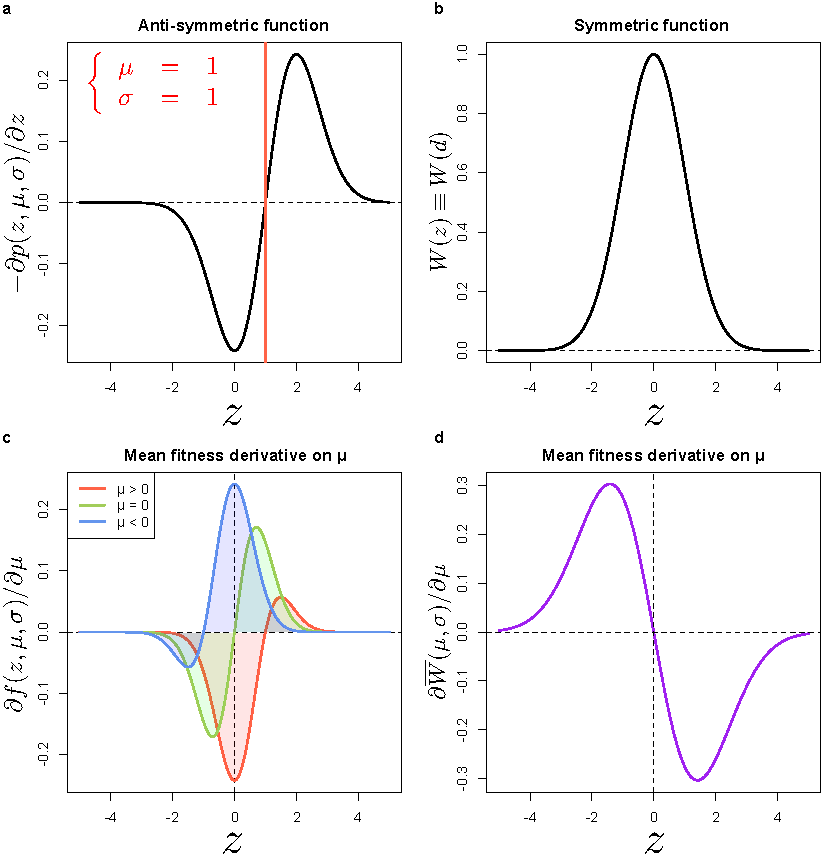
\includegraphics[scale=1]{part1_appendixS3_fig1.pdf}
\end{adjustwidth}
\caption[Behavior of $\partial \overline{W}(\mu,\sigma)/\partial \mu$.]{
\textbf{Behavior of $\partial \overline{W}(\mu,\sigma)/\partial \mu$.}
\textbf{a,} The normal distribution derivative $-\partial p(z,\mu,\sigma)/\partial z$ is an anti-symmetric function centered on $z=\mu$, such that the function is negative when $z < \mu$ and positive when $z > \mu$. Here, an example is given for $\mu=1$ and $\sigma=1$. The red vertical line represents the value of $\mu$, which is an axis of symmetry of the function.
\textbf{b,} The Gaussian-shaped fitness function $W(z)$ is a strictly positive, symmetric function centered on $z=0$.
\textbf{c,d,} The product of both functions, equal to $\partial f(z,\mu,\sigma)/\partial \mu$ is biased towards positive values if $\mu < 0$ (blue curve), towards negative values if $\mu > 0$ (red curve), or anti-symmetric if $\mu=0$ (green curve). Thus the integral $\int_z \partial f(z,\mu,\sigma)/\partial \mu\ dz$ is respectively positive, negative, or zero, if $\mu$ is negative, positive or zero (as shown in panel \textbf{d}, purple curve).
}
\label{part1:appendixS3:fig1}
\end{figure}

\begin{figure}[!h]
\begin{adjustwidth}{-0in}{0in}
\centering
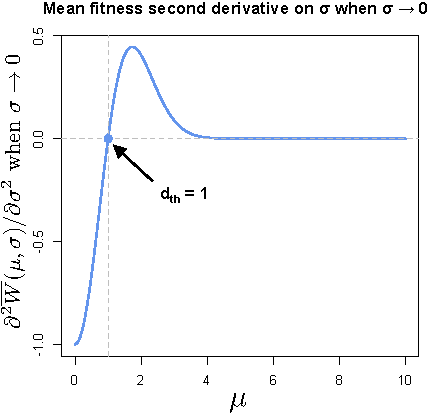
\includegraphics[scale=1]{part1_appendixS3_fig2.pdf}
\end{adjustwidth}
\caption[Variation of $\partial^2 W(\mu,\sigma)/\partial \sigma^2$ when $\sigma \rightarrow 0$.]{
\textbf{Variation of $\partial^2 \overline{W}(\mu,\sigma)/\partial \sigma^2$ when $\sigma \rightarrow 0$.}
The variation of $\partial^2 \overline{W}(\mu,\sigma)/\partial \sigma^2$ when $\sigma \rightarrow 0$ is represented here depending on $\mu$. It is described by Equation \ref{eq:part1:d2wdsigma}. Blue dot: inflection point of the ridge $\partial \overline{W}(\mu,\sigma)/\partial \sigma = 0$ (Fig. \ref{part1:appendixS3:fig3} orange circle), for $\mu = d_{th} = 1$.
}
\label{part1:appendixS3:fig2}
\end{figure}

\begin{figure}[!h]
\begin{adjustwidth}{-0in}{0in}
\centering
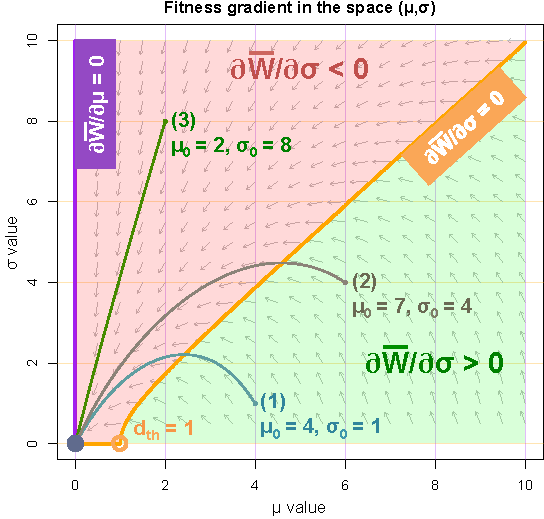
\includegraphics[scale=1]{part1_appendixS3_fig3.pdf}
\end{adjustwidth}
\caption[Variations of the mean fitness $\overline{W}(\mu,\sigma)$ in the space $(\mu,\sigma)$.]{\textbf{Variations of the mean fitness $\overline{W}(\mu,\sigma)$ in the space $(\mu,\sigma)$.}
In purple, the ridge $\partial \overline{W}/\partial \mu=0$. In orange, the ridge $\partial \overline{W}/\partial \sigma=0$. Green area: $\partial \overline{W}/\partial \sigma > 0$ (\textit{i.e.}, it is beneficial to increase the phenotypic noise). Red area: $\partial \overline{W}/\partial \sigma < 0$ (\textit{i.e.}, it is beneficial to reduce the phenotypic noise). Three trajectories following the fitness gradient are represented \textbf{(1)} in blue (initial values: $\mu_0=4, \sigma_0=1$), \textbf{(2)} in brown (initial values: $\mu_0=6, \sigma_0=4$) and \textbf{(3)} in green (initial values: $\mu_0=2, \sigma_0=8$). Black dot: fitness optimum $z_{opt}$. Orange circle: inflection point $d_{th}=1$ of the fitness landscape $W(z)$. Grey arrows indicate the direction of the fitness gradient, but not its amplitude.
}
\label{part1:appendixS3:fig3}
\end{figure}

%%%%%%%%%%%%%%%%%%%%%%%%%%%%%%%%%%%%%%%%%%%%
%%%%%%%%%%%%%%%%%%%%%%%%%%%%%%%%%%%%%%%%%%%%

The second derivative of $f$ then reads:
\begin{equation}
\begin{array}{rcl}
\dfrac{\partial^2 f(z,\mu,\sigma)}{\partial \sigma^2} & = & \dfrac{(z-\mu)^2-\sigma^2}{\sigma^3} f(z,\mu,\sigma) + \left( \dfrac{\sigma^2-3(z-\mu)^2}{\sigma^4}\right)^2 f(z,\mu,\sigma)\\\\
& = & f(z,\mu,\sigma) \left( \dfrac{\sigma^4-3\sigma^2(z-\mu)^2+(z-\mu)^4-2(z-\mu)^2\sigma^2+\sigma^4}{\sigma^6} \right)\\\\
& = & f(z,\mu,\sigma) \left( \dfrac{2\sigma^4-5(z-\mu)^2\sigma^2+(z-\mu)^4}{\sigma^6} \right).
\end{array}
\end{equation}
As demonstrated previously, it is possible to rewrite this equation to extract derivatives of normal law densities:
\begin{equation}
\begin{array}{rcl}
\dfrac{\partial^2 f(z,\mu,\sigma)}{\partial \sigma^2} & = & f(z,\mu,\sigma) \left( \dfrac{(z-\mu)^4-6(z-\mu)^2\sigma^2+3\sigma^4}{\sigma^6}+\dfrac{(z-\mu)^2\sigma^2-\sigma^4}{\sigma^6} \right)\\\\
& = & \sigma^2\ f(z,\mu,\sigma) \left( \dfrac{(z-\mu)^4-6(z-\mu)^2\sigma^2+3\sigma^4}{\sigma^8} + \dfrac{1}{\sigma^2}\dfrac{(z-\mu)^2-\sigma^2}{\sigma^4} \right)\\\\
& = & \sigma^2\ f(z,\mu,\sigma) \left( \dfrac{(z-\mu)^4-6(z-\mu)^2\sigma^2+3\sigma^4}{\sigma^8} + \dfrac{(z-\mu)^2-\sigma^2}{\sigma^6} \right)\\\\
& = & \sigma^2\ W(z) \left( \dfrac{\partial^4 p(z,\mu,\sigma)}{\partial z^4} + \dfrac{1}{\sigma^2} \times \dfrac{\partial^2 p(z,\mu,\sigma)}{\partial z^2} \right)\\\\
& = & \underbrace{\left( \sigma^2\ W(z) \dfrac{\partial^4 p(z,\mu,\sigma)}{\partial z^4} \right)}_{\rightarrow 0 \text{ when } \sigma \rightarrow 0} + \left(W(z) \dfrac{\partial^2 p(z,\mu,\sigma)}{\partial z^2} \right).
\end{array}
\label{eq:part1:second_derivative}
\end{equation}

Consequently, when $\sigma \rightarrow 0$, the partial derivative $\partial^2 \overline{W}(\mu,\sigma)/\partial \sigma^2$ reads:
\begin{equation}
\lim\limits_{x \to 0}\ \dfrac{\partial^2 \overline{W}(\mu,\sigma)}{\partial \sigma^2} = (\mu^2-1)\ W(\mu).
\label{eq:part1:d2wdsigma}
\end{equation}

The only value of $\mu$ for which $\partial^2 \overline{W}(\mu,\sigma)/\partial \sigma^2 = 0$ is $|\mu| = 1$. When $|\mu| < 1$, $\partial^2 \overline{W}(\mu,\sigma)/\partial \sigma^2 < 0$, meaning that the selective pressure is towards a reduction of the phenotypic noise $\sigma$. When $|\mu| > 1$, $\partial^2 \overline{W}(\mu,\sigma)/\partial \sigma^2 > 0$, meaning that the selective pressure is towards an increase of the phenotypic noise $\sigma$ (Fig. \ref{part1:appendixS3:fig2} blue curve, and Fig. \ref{part1:appendixS3:fig3} orange curve and circle). Thus, $d_{th}=1$.

%%%%%%%%%%%%%%%%%
%%%%%%%%%%%%%%%%%

\section*{Analytical and numerical studies of an isotropic noise on $n$ phenotypic characters}

As described in Results, an isotropic noise is applied to the mean phenotype $\boldsymbol{\mu}$, by independently varying each trait value $\mu_i$ with the same noise amplitude $\sigma$. The probability $p(\boldsymbol{z},\boldsymbol{\mu},\sigma)$ for an organism $(\boldsymbol{\mu}, \sigma)$ to express the phenotype $\boldsymbol{z}$ is then:
\begin{equation}
p(\boldsymbol{z},\boldsymbol{\mu},\sigma) = \prod_{i \in n} \dfrac{1}{\sigma \sqrt{2\pi}} \exp \left[ \dfrac{-(z_i-\mu_i)^2}{2\sigma^2} \right].
\end{equation}

As in the previous section, the goal is to compute the second derivative of $\overline{W}(\boldsymbol{\mu}, \sigma)$ on $\sigma$, and find its inflection point to detect the critical euclidean distance $d_{th}$ below which phenotypic noise must be minimized. However, we now must compute it in $n$ dimensions. Hopefully, two conditions allow us to strongly simplify the equations:
\begin{enumerate}
\item[\textbf{(1)}] Noise is isotropic, such that $\overline{W}(\boldsymbol{\mu}, \sigma)$ can be decomposed in a product of one-dimensional integrals;
\item[\textbf{(2)}] The mean phenotype of an organism $\boldsymbol{\mu}$ is taken away from the fitness optimum on a single axis, all other axes remaining at a distance zero of the fitness optimum. By rotational symmetry, we can generalize to any position $\boldsymbol{\mu}$ away from the fitness optimum.
\end{enumerate}

$\overline{W}(\boldsymbol{\mu}, \sigma)$ reads:
\begin{equation}
\begin{array}{rcl}
\overline{W}(\boldsymbol{\mu}, \sigma) & = & \displaystyle\int_{\mathbb{R}^n} p(\boldsymbol{z},\boldsymbol{\mu},\sigma)W(\boldsymbol{z})d\boldsymbol{z}\\\\
& = & \displaystyle\int_{\mathbb{R}} p(z_1,\mu_1,\sigma)W(z_1)dz_1 \times ... \times \displaystyle\int_{\mathbb{R}} p(z_n,\mu_n,\sigma)W(z_n)dz_n.
\end{array}
\end{equation}

If we only move the mean phenotypic trait value $\mu_1$ away from the fitness optimum, all other mean trait values being equal to zero, $\overline{W}(\boldsymbol{\mu}, \sigma)$ then reads:
\begin{equation}
\begin{array}{rcl}
\overline{W}(\boldsymbol{\mu}, \sigma) & = & \displaystyle\int_{\mathbb{R}} p(z_1,\mu_1,\sigma)W(z_1)dz_1 \times \left( \displaystyle\int_{\mathbb{R}} p(z,0,\sigma)W(z)dz \right)^{n-1}.
\end{array}
\end{equation}

As demonstrated above, we know that for a single character and when $\sigma \rightarrow 0$, the successive derivatives of $\overline{W}(\mu, \sigma)$ read:
\begin{equation}
\left\{
\begin{array}{ccl}
\overline{W} & = & W(\mu)\\\\
\overline{W}' & = & 0\\\\
\overline{W}'' & = & (\mu^2-1)W(\mu)
\end{array}
\right.
\label{eq:part1:derivative1}
\end{equation}

Moreover, when $\mu = 0$, we find that:
\begin{equation}
\left\{
\begin{array}{ccl}
\overline{W}_0 & = & 1\\\\
\overline{W}_0' & = & 0\\\\
\overline{W}_0'' & = & -1
\end{array}
\right.
\label{eq:part1:derivative2}
\end{equation}

We then define the terms $a$, $b$ and $c$ such that:
\begin{equation}
\left\{
\begin{array}{ccl}
a & = & \displaystyle\int_{\mathbb{R}} p(z_1,\mu_1,\sigma)W(z_1)dz_1\\\\
b & = & \displaystyle\int_{\mathbb{R}} p(z,0,\sigma)W(z)dz\\\\
c & = & b^{\ n-1}
\end{array}
\right.
\end{equation}

We now compute the second derivative of $\overline{W}(\boldsymbol{\mu}, \sigma)$ on $\sigma$, according to $a$, $b$ and $c$, this equation reads:
\begin{equation}
\dfrac{\partial^2 \overline{W}(\boldsymbol{\mu}, \sigma)}{\partial \sigma^2} = ac'' + 2a'c' + a''c
\end{equation}
With:
\begin{equation}
\left\{
\begin{array}{ccl}
c' & = & (n-1)b'b^{\ n-2}\\\\
c'' & = & (n-1)(n-2)b'b^{\ n-3} + (n-1)b''b^{\ n-2}
\end{array}
\right.
\end{equation}

Then, the complete equation of $\partial \overline{W}(\boldsymbol{\mu}, \sigma) / \partial \sigma$ reads:
\begin{equation}
\begin{array}{rcl}
\dfrac{\partial^2 \overline{W}(\boldsymbol{\mu}, \sigma)}{\partial \sigma^2} & = & a \left( (n-1)(n-2)b'b^{\ n-3} + (n-1)b''b^{\ n-2} \right)\\\\
& + & 2a'(n-1)b'b^{\ n-2}\\\\
& + & a''b^{\ n-1}.
\end{array}
\end{equation}

We now replace the terms $a$ and $b$ by the corresponding terms in Equations \ref{eq:part1:derivative1} and \ref{eq:part1:derivative2}:

\begin{equation}
\begin{array}{rcl}
\dfrac{\partial^2 \overline{W}(\boldsymbol{\mu}, \sigma)}{\partial \sigma^2} & = & \overline{W} \left( (n-1)(n-2)\overline{W}_0'\overline{W}_0^{\ n-3} + (n-1)\overline{W}_0''\overline{W}_0^{\ n-2} \right)\\\\
& + & 2\overline{W}'(n-1)\overline{W}_0'\overline{W}_0^{\ n-2}\\\\
& + & \overline{W}''\overline{W}_0^{\ n-1}.
\end{array}
\end{equation}

Finally, the second derivative of $\overline{W}(\boldsymbol{\mu}, \sigma)$ on $\sigma$ reads:
\begin{equation}
\dfrac{\partial^2 \overline{W}(\boldsymbol{\mu}, \sigma)}{\partial \sigma^2} = (\mu_1^2-n)W(\mu_1).
\label{eq:part1:super_equation}
\end{equation}

The only value of $\mu_1$ for which Equation \ref{eq:part1:super_equation} is equal to zero is $\mu_1 = \pm \sqrt{n}$. Since this result is valid when the euclidean distance $d = \lVert \boldsymbol{\mu} \rVert$ is equal to $\sqrt{n}$, we can conclude that the critical distance below which isotropic phenotypic noise must be minimized is $d_{th} = \sqrt{n}$.

%%%%%%%%%%%%%%%%%
%%%%%%%%%%%%%%%%%

\section*{Anisotropic and correlated phenotypic noise is beneficial when aligned with the fitness optimum}

Let us consider the organism $(\boldsymbol{\mu}, \boldsymbol{\sigma}, \boldsymbol{\theta})$ in a $n$-dimensional phenotypic space, sitting at a certain distance of the fitness optimum $\boldsymbol{z_{opt}}$ (beyond $d_{th}=\sqrt{n}$) and evolving towards it. We describe the phenotypic noise of this organism by a multivariate normal distribution $\mathcal{N}_n(\boldsymbol{\mu},\boldsymbol{\Sigma})$. This multivariate normal distribution can be represented by an hyper-ellipse in $\mathbb{R}^n$, as shown in Figure \ref{part1:appendixS3:fig4} for two dimensions.

We now define the axes $\boldsymbol{v_1}, ..., \boldsymbol{v_n}$ (the origin of the new basis also being $\boldsymbol{\mu}$), with $\boldsymbol{v_1}$ aligned towards the fitness optimum $\boldsymbol{z_{opt}}$, all other axes $\boldsymbol{v_i}$ being orthogonal to $\boldsymbol{v_1}$ (Fig. \ref{part1:appendixS3:fig4}a).
Along axis $\boldsymbol{v_1}$, the organism $(\boldsymbol{\mu}, \boldsymbol{\sigma}, \boldsymbol{\theta})$ experiences a convex fitness if $\lVert \boldsymbol{\mu} \rVert > 1$. Along all other axes $\boldsymbol{v_i}$, the organism experiences a concave fitness, sitting at a local optimum in all cases (Fig. \ref{part1:appendixS3:fig4}b).
The basis associated to axes $\boldsymbol{v_1}, ..., \boldsymbol{v_n}$ is the orthonormal matrix $\boldsymbol{V}$ of size $n \times n$, where $\boldsymbol{v_1}$ is defined by the vector $\boldsymbol{\mu}$. By defining $\overline{\boldsymbol{\mu}} = \boldsymbol{\mu}/\lVert \boldsymbol{\mu} \rVert$, the matrix $\boldsymbol{V}$ reads:
\begin{equation}
\boldsymbol{V} = 
\begin{pmatrix}
\left. \overline{\boldsymbol{\mu}} \right| ... 
\end{pmatrix}
\end{equation}

The goal here is to find the phenotypic noise configuration that maximizes the expected fitness $\overline{W}(\boldsymbol{\mu}, \boldsymbol{\Sigma})$, knowing that:
\begin{equation}
\overline{W}(\boldsymbol{\mu}, \boldsymbol{\Sigma}) = \int_{\mathbb{R}^n} p(\boldsymbol{z},\boldsymbol{\mu},\boldsymbol{\Sigma})W(\boldsymbol{z})d\boldsymbol{z}.
\end{equation}

We first make a variable change by defining $\boldsymbol{\epsilon}$ such that the realized phenotype $\boldsymbol{z} = \boldsymbol{\mu}+\boldsymbol{\epsilon}$. Thus:
\begin{equation}
\overline{W}(\boldsymbol{\mu}, \boldsymbol{\Sigma}) = \int_{\mathbb{R}^n} p(\boldsymbol{\epsilon},\boldsymbol{0},\boldsymbol{\Sigma})W(\boldsymbol{\mu}+\boldsymbol{\epsilon})d\boldsymbol{\epsilon}.
\label{eq:part1:Wbar_epsilon}
\end{equation}
According to our previous results, we know that if $\lVert \boldsymbol{\mu} \rVert > 1$, phenotypic noise is beneficial along $\boldsymbol{v_1}$ axis, where $W(\boldsymbol{z})$ is convex, and is deleterious along all other orthogonal axes of $\boldsymbol{V}$ (Fig. \ref{part1:appendixS3:fig4}b).
Thus, for any covariance matrix $\boldsymbol{\Sigma}$ and for any $\boldsymbol{\epsilon} \sim \mathcal{N}_n(\boldsymbol{0},\boldsymbol{\Sigma})$, the fitness $W(\boldsymbol{\mu}+\boldsymbol{\epsilon})$of the expressed phenotype $\boldsymbol{z} = \boldsymbol{\mu},\boldsymbol{\epsilon}$ is always lower or equal to the fitness of its projection along axis $\boldsymbol{v_1}$ (\textit{i.e.}, the distance towards the optimum will always be shorter or equal for the projection). Thus:
\begin{equation}
\int_{\mathbb{R}^n} p(\boldsymbol{\epsilon},\boldsymbol{0},\boldsymbol{\Sigma})W(\boldsymbol{\mu}+\boldsymbol{\epsilon})d\boldsymbol{\epsilon}
\leq
\int_{\mathbb{R}^n} p(\boldsymbol{\epsilon},\boldsymbol{0},\boldsymbol{\Sigma})W(\boldsymbol{\mu}+\overline{\boldsymbol{\mu}}^T\boldsymbol{\epsilon}\overline{\boldsymbol{\mu}})d\boldsymbol{\epsilon}.
\label{eq:part1:inequality1}
\end{equation}

We then express $\boldsymbol{\epsilon}$ in the basis $\boldsymbol{V}$ by making the following variable change: $\boldsymbol{s} = \boldsymbol{V}^T \boldsymbol{\epsilon}$. Consequently, $\boldsymbol{\epsilon} = \boldsymbol{V}\!\boldsymbol{s}$, such that:
\begin{equation}
\begin{array}{rcl}
\overline{\boldsymbol{\mu}}^T\boldsymbol{\epsilon}\overline{\boldsymbol{\mu}} & = & \overline{\boldsymbol{\mu}}^T\boldsymbol{V}\boldsymbol{s}\overline{\boldsymbol{\mu}}\\\\
& = & s_1 \overline{\boldsymbol{\mu}}.
\end{array}
\end{equation}

We can rewrite the right term of the Equation \ref{eq:part1:inequality1} as following:
\begin{equation}
\int_{\mathbb{R}^n} p(\boldsymbol{V}\!\boldsymbol{s},\boldsymbol{0},\boldsymbol{\Sigma}) \underbrace{W(\boldsymbol{\mu}+s_1 \overline{\boldsymbol{\mu}})}_{\text{Only depends on $s_1$}}ds_1, ..., ds_n.
\label{eq:part1:mega_integral1}
\end{equation}
The term $W(\boldsymbol{\mu}+s_1 \overline{\boldsymbol{\mu}})$ only depending on $s_1$, we can extract it from the integral by writing:
\begin{equation}
\int_{\mathbb{R}} W(\boldsymbol{\mu}+s_1 \overline{\boldsymbol{\mu}}) \left[\int_{\mathbb{R}^{n-1}} p(\boldsymbol{V}\!\boldsymbol{s},\boldsymbol{0},\boldsymbol{\Sigma}) ds_2, ..., ds_n \right] ds_1.
\label{eq:part1:mega_integral2}
\end{equation}

The probability density function $p(\boldsymbol{V}\!\boldsymbol{s},\boldsymbol{0},\boldsymbol{\Sigma})$ from Equation \ref{eq:part1:mega_integral2} is strictly equivalent to $p(\boldsymbol{s},\boldsymbol{0},\boldsymbol{V}^T\boldsymbol{\Sigma}\boldsymbol{V})$ (demonstration not shown here).
In this case, the inner integral of Equation \ref{eq:part1:mega_integral2} reads:
\begin{equation}
\int_{\mathbb{R}^{n-1}} p(\boldsymbol{s},\boldsymbol{0},\boldsymbol{V}^T\boldsymbol{\Sigma}\boldsymbol{V}) ds_2, ..., ds_n.
\label{eq:part1:mega_integral3}
\end{equation}
This equation (Eq. \ref{eq:part1:mega_integral3}) describes the marginal density of $s_1$, following the univariate normal law:
\begin{equation}
s_1 \sim \mathcal{N}(0, \left[\boldsymbol{V}^T\boldsymbol{\Sigma}\boldsymbol{V}\right]_{1,1})
\label{eq:part1:univariate1}
\end{equation}
the subscript ``$1,1$'' denoting the coefficient of the first raw and first column.

Then, Equation \ref{eq:part1:mega_integral3} reads:
\begin{equation}
\int_{\mathbb{R}} W(\boldsymbol{\mu}+s_1 \overline{\boldsymbol{\mu}}) p(s_1,0,\left[\boldsymbol{V}^T\boldsymbol{\Sigma}\boldsymbol{V}\right]_{1,1}) ds_1.
\label{eq:part1:mega_integral4}
\end{equation}
Note that, by rotational symmetry, $W(\boldsymbol{\mu}+s_1 \overline{\boldsymbol{\mu}}) = W((\lVert \boldsymbol{\mu} \rVert + s_1)\boldsymbol{e_1})$, because vectors $\boldsymbol{\mu}$ and $\overline{\boldsymbol{\mu}}$ are aligned. Thus, Equation \ref{eq:part1:mega_integral4} is just the one dimensional expected fitness $\overline{W}(\lVert \boldsymbol{\mu} \rVert, \left[\boldsymbol{V}^T\boldsymbol{\Sigma}\boldsymbol{V}\right]_{1,1})$. Previous results demonstrated that along axis $\boldsymbol{v_1}$, phenotypic noise properties can be described in one dimension, such that there is an optimal value $\left[\boldsymbol{V}^T\boldsymbol{\Sigma}\boldsymbol{V}\right]_{1,1} = \sigma_{opt}^2$ that maximizes the expected fitness $\overline{W}(\lVert \boldsymbol{\mu} \rVert, \left[\boldsymbol{V}^T\boldsymbol{\Sigma}\boldsymbol{V}\right]_{1,1})$. This leads to the inequality:
\begin{equation}
\overline{W}(\lVert \boldsymbol{\mu} \rVert, \left[\boldsymbol{V}^T\boldsymbol{\Sigma}\boldsymbol{V}\right]_{1,1}) = \int_{\mathbb{R}} W(z) p(z,\lVert \boldsymbol{\mu} \rVert,\left[\boldsymbol{V}^T\boldsymbol{\Sigma}\boldsymbol{V}\right]_{1,1}) dz
\leq
\overline{W}(\lVert \boldsymbol{\mu} \rVert, \sigma_{opt}^2).
\label{eq:part1:inequalitybis}
\end{equation}

By decomposing the covariance matrix $\boldsymbol{\Sigma}$ in its eigenvalues $\boldsymbol{\sigma}^2$, such that $\boldsymbol{\Sigma} = \boldsymbol{U}\boldsymbol{D}\boldsymbol{U}^T$, we obtain:
\begin{equation}
\boldsymbol{V}^T\boldsymbol{\Sigma}\boldsymbol{V} = \boldsymbol{V}^T\boldsymbol{U}\boldsymbol{D}\boldsymbol{U}^T\boldsymbol{V}.
\label{eq:part1:sigma_decomposition}
\end{equation}
If the eigenvector $\boldsymbol{u_1}$ of $\boldsymbol{U}$ (Fig. \ref{part1:appendixS3:fig4}a) is aligned with the axis $\boldsymbol{v_1}$ of the basis $\boldsymbol{V}$, then the best phenotypic noise configuration is to have $\boldsymbol{\sigma}^2 = \{\sigma_{opt}^2, 0, ..., 0\}$ (with $\boldsymbol{D} = \mathrm{diag}(\boldsymbol{\sigma}^2)$).

As a whole, our analytical study led to two important inequalities described in Equations \ref{eq:part1:inequality1} and \ref{eq:part1:inequalitybis}. 
For any organism $(\boldsymbol{\mu}, \boldsymbol{\sigma}, \boldsymbol{\theta})$ where $\lVert \boldsymbol{\mu} \rVert > 1$, the first inequality (Eq. \ref{eq:part1:inequality1}) demonstrates that it is always preferable to not have positive phenotypic noise that is not aligned with the fitness optimum (\textit{i.e.}, along the axis $\boldsymbol{v_1}$).
However, if none of the principal components $\boldsymbol{u_i}$ of the covariance matrix $\boldsymbol{\Sigma}$ are aligned with the fitness optimum, this optimal scenario is unreachable because there is always positive phenotypic noise orthogonal to the direction of the fitness optimum $\boldsymbol{u_i}$ (the inequality \ref{eq:part1:inequality1} is strict).
On the contrary, if one of the principal components $\boldsymbol{u_1}$ is aligned with the fitness optimum, it is possible to minimize orthogonal noise components (the inequality \ref{eq:part1:inequality1} is not strict).

Moreover, in the case where $\boldsymbol{u_1}$ is aligned with the fitness optimum and if orthogonal noise components are set to zero (\textit{i.e.}, phenotypic noise is one-dimensional), results presented above show that it exists an optimal noise amplitude $\sigma_{opt}^2$ that maximizes the one dimensional expected fitness $\overline{W}(\lVert \boldsymbol{\mu} \rVert, \left[\boldsymbol{V}^T\boldsymbol{\Sigma}\boldsymbol{V}\right]_{1,1})$. This corresponds to setting all the eigenvalues of $\boldsymbol{\Sigma}$ to zero, except the one associated to $\boldsymbol{u_1}$, that is equal to $\sigma_{opt}^2$.

\begin{figure}[!h]
\begin{adjustwidth}{-0.4in}{0in}
\centering
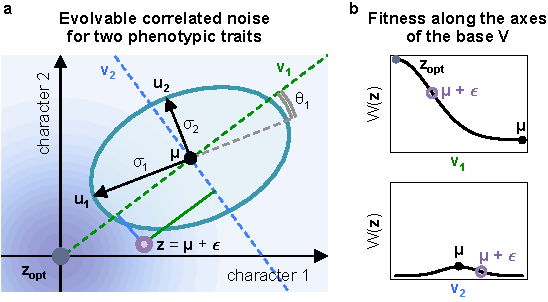
\includegraphics[scale=1.5]{part1_appendixS3_fig4.pdf}
\end{adjustwidth}
\caption[Anisotropic and correlated phenotypic noise for two traits.]{\textbf{Anisotropic and correlated phenotypic noise for two traits.}
\textbf{a,} The phenotypic distribution of an organism $(\boldsymbol{\mu}, \boldsymbol{\sigma}, \boldsymbol{\theta})$ is defined by a multivariate normal distribution with mean $\boldsymbol{\mu}$ (black dot), noise amplitudes $\sigma_1$ and $\sigma_2$ (black arrows) along axes $\boldsymbol{u_1}$ and $\boldsymbol{u_2}$, and a parameter of correlation $\theta_1$ (grey angle), defining a rotation of the basis $\boldsymbol{U} = (\boldsymbol{u_1}, \boldsymbol{u_2})$. A phenotype $\boldsymbol{z}$ (purple dot) is generated from the multivariate normal distribution by drawing a random vector $\boldsymbol{\epsilon} \sim \mathcal{N}_n(\boldsymbol{0},\boldsymbol{\Sigma})$ (with $\boldsymbol{\Sigma}$ the covariance matrix built from $\boldsymbol{\sigma}$ and $\boldsymbol{\theta}$), such that $\boldsymbol{z} = \boldsymbol{\mu} + \boldsymbol{\epsilon}$. The contribution of $\boldsymbol{\epsilon}$ on each axis $\boldsymbol{v_1}$ (in green) and $\boldsymbol{v_2}$ (in blue) of the basis $\boldsymbol{V}$, where $\boldsymbol{v_1}$ is aligned with the fitness optimum $\boldsymbol{z_{opt}}$, is represented by the vector $\boldsymbol{s} = (s_1, s_2)^T$. The fitness landscape is represented by a gradient of blue centered on the fitness optimum $\boldsymbol{z_{opt}}$ (blue dot).
\textbf{b,} Fitness along axes of the basis $\boldsymbol{V} = (\boldsymbol{v_1}, \boldsymbol{v_2})$. Along axis $\boldsymbol{v_1}$, aligned with the fitness optimum $\boldsymbol{z_{opt}}$, the organism experiences a convex fitness (if $\lVert \boldsymbol{\mu} \rVert > 1$). Along axis $\boldsymbol{v_2}$, orthogonal to $\boldsymbol{v_1}$, the organism a concave fitness, sitting on a local fitness optimum.
}
\label{part1:appendixS3:fig4}
\end{figure}

%%%%%%%%%%%%%%%%%
%%%%%%%%%%%%%%%%%

\section*{Concluding remarks}

Our demonstrations mainly rely on the study of the local convexity of the fitness function. As such, any function admitting the same properties as $W(\boldsymbol{z})=\exp\left[-\boldsymbol{z}^2/2\right]$ (\textit{i.e.}, a positive function being concave at the optimum and admitting one convex inflection point) will give the same general results. Moreover, in our study, phenotypic noise and mutation distributions are Gaussian-shaped. As demonstrated above, this choice allowed us to obtain precise analytical results.



\newpage

%%%%%%%%%%%%%%%%%%%%%%%%%%%

\subsection{Data S1. Phenotypic noise correlations matrices of each replicate of the 37 strains of yeast in Fisher's space.}
\label{part1:DataS1}

\href{https://github.com/charlesrocabert/SigmaFGM/tree/master/phenomics\_analysis/DataS1.zip}{https://github.com/charlesrocabert/SigmaFGM/tree/master/phenomics\_analysis/DataS1.zip}

\newpage

%%%%%%%%%%%%%%%%%%%%%%%%%%%

\subsection{Data S2. Phenotypic noise correlations matrices of each of the 37 strains of yeast in Fisher's space, with Pearson correlation tests.}
\label{part1:DataS2}

\href{https://github.com/charlesrocabert/SigmaFGM/tree/master/phenomics\_analysis/DataS1.zip}{https://github.com/charlesrocabert/SigmaFGM/tree/master/phenomics\_analysis/DataS2.zip}

\newpage

%%%%%%%%%%%%%%%%%%%%%%%%%%%

\subsection{Script S1. A numerical solver for {\sigmaFGM}.}
\label{part1:ScriptS1}

\href{https://github.com/charlesrocabert/SigmaFGM}{https://github.com/charlesrocabert/SigmaFGM}

\newpage

%%%%%%%%%%%%%%%%%%%%%%%%%%%

\subsection{Script S2. Phenomics analysis of 37 strains of yeast.}
\label{part1:ScriptS2}

\href{https://github.com/charlesrocabert/SigmaFGM/tree/master/phenomics\_analysis}{https://github.com/charlesrocabert/SigmaFGM/tree/master/phenomics\_analysis}

\newpage

%%%%%%%%%%%%%%%%%%%%%%%%%%%









%%%%%%%%%%%%%%%%%%%%%%%%%% PART 2 %

\part{An \textit{in silico} experimental evolution approach to study Evolution of Evolution}
\label{part2}


%%%%%%%%%%%%%%%
%%%      CHAPTER      %%%
%%%%%%%%%%%%%%%

\chapter{{\EvoEvoSim}, a multi-scale model dedicated to Evolution of Evolution}
\label{ch:part2:methodology}

\paragraph{}
\paragraph{}
\paragraph{}
\paragraph{}
\paragraph{}
\paragraph{}
\paragraph{}
\begin{center}
\large \textbf{The development of {\EvoEvoSim} is part of the European project EvoEvo (FP7-ICT-610427). The description of work of the project and the deliverables related to {\EvoEvoSim} are freely available at \href{www.evoevo.eu}{www.evoevo.eu}.}
\end{center}

\newpage

%%%%%%%%%%%%%%%%%%%%%%%%% SECTION : INTRODUCTION %

\begin{quote}
Although there has been much discussion on what is the appropriate level on which Darwinian selection operates, we now know that in many cases the interesting features arise through the occurrence of multiple levels of selection which act in concordance and/or in conflict.\\
\citep{hogeweg-and-takeuchi-2003}
\end{quote}

\section{Meet {\EvoEvoSim}}
\label{sec:part2:methodology:intro}

\begin{figurehere}
\centerline{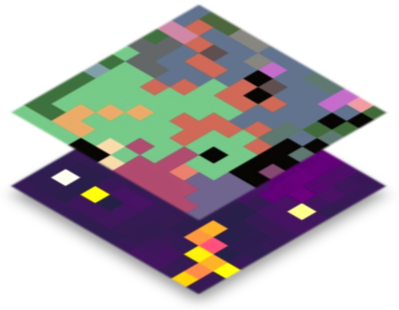
\includegraphics[width=0.2\textwidth]{part2_logo_evo2sim.png}}
\caption{{\EvoEvoSim} logo.}
\end{figurehere}

{\EvoEvoSim} is a \textbf{multi-scale} and \textbf{individual-based} model of evolution, inspired from \textbf{pearls-on-a-string} \citep{crombach-hogeweg-2008} and \textbf{sequence-of-nucleotides} \citep{beslon-et-al-2010a,hindre-et-al-2012}.
As discussed in introduction, developing complex representations of the genotype-to-phenotype map and fitness landscape has been a primary goal in the conception of this model. To do so, we used the \textbf{bag-of-tuples} formalism (also discussed in introduction) to develop an  \textbf{artificial chemistry} allowing for multi-level evolution. 

Two major objectives constrained the development of {\EvoEvoSim}: \textbf{(i)} integrate a maximum number of pertinent biological structures and levels (genome, genetic regulation, metabolic network, cell, population, ...) to enable deep exploration of EvoEvo, and \textbf{(ii)} maintain the model complexity low enough to enable its practical use. As such, a tough compromise had to be made between the degree of realism (the number of assumptions we want to pick to build the model, see \citealt{servedio-et-al-2014}), and what we want the model to tell us. This modeling problem is well-resumed by the concept of Medawar zone: as illustrated in Figure \ref{fig:part2:methodology:medawar_zone}, the Medawar zone is the area where the model complexity is most likely to produce fruitful results. Too simple models are unlikely to produce novel or significant results. Too complex models may not succeed at all or may be rejected by the research community at large \citep{loehle-1990}.
\begin{figure}[!ht]
\centering
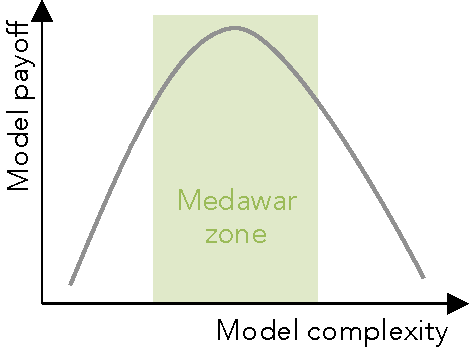
\includegraphics[width=0.4\textwidth]{part2_medawarzone.pdf}
\caption[The Medawar zone.]{\textbf{The Medawar zone.} The Medawar zone is the area where the model complexity is most likely to produce fruitful results. Too simple models are unlikely to produce novel or significant results. Too complex models may not succeed at all or may be rejected by the research community at large \citep{loehle-1990}.}
\label{fig:part2:methodology:medawar_zone}
\end{figure}

As described in the description of work of the EvoEvo project\footnote{Available at \href{www.evoevo.eu}{www.evoevo.eu}}, a primary objective in the development of {\EvoEvoSim} was to merge the R-{\aevol} model \citep{beslon-et-al-2010a}, which includes a complex representation of the genome and the genetic regulation network, with the pearls-on-a-string formalism, which is very flexible and allows for vast modeling possibilities at the level of the regulation and the metabolism \citep{crombach-hogeweg-2007,crombach-hogeweg-2008,crombach-hogeweg-2009}.
Six biological structures have been modeled in {\EvoEvoSim}.
\textbf{(i)} The \textbf{genome} encodes two interlaced networks: \textbf{(ii)} the \textbf{genetic regulatory network}, that controls gene expression, and \textbf{(iii)} the \textbf{metabolic network}, that allows the cell to perform tasks in interaction with the environment. \textbf{(iv)} Together, these three first levels form the fourth one: the \textbf{cell}. By uptaking, transforming and releasing metabolites (actively or at death), the cell grows, and produces material necessary to its division.
\textbf{(v)} Living cells compose the \textbf{population}, and evolve in \textbf{(vi)} a two dimensional \textbf{environment}, in which free metabolites diffuse and degrade over time.

The fitness of each organism depends on the production of essential metabolites, built from available resources in the local environment. Doing so, organisms constantly modify their environment, thus perturbing selective pressures. Free metabolites can be depleted, new unseen free metabolites can appear in the environment, resources can cycle, and so on. The fitness landscape is then completely dependent on the interaction between the population and the environment, and is evolvable. In this sense, it could be more appropriate to use the term \textbf{fitness seascape} to render the fluctuating selective pressures \citep{mustonen-lassig-2009}.

In the following section, the modeling choices for the artificial chemistry, the genotype-to-phenotype map and the fitness landscape will be described in more details.

%%%%%%%%%%%%%%%%%%%%%%%%% SECTION : THE GENOME %

\section{The genome}
\label{sec:part2:methodology:genome}

%%%%%%%%%%%%%

\subsection{Genome structure}
\label{subsec:part2:methodology:genome_structure}

In {\EvoEvoSim}, the genome structure mimics bacterial genomes organization, with some simplifications. Following the pearls-on-a-string formalism, the resolution of genomic sequences is coarse-grained: no nucleotides representation here, a sequence is made of \textbf{genetic units}, somehow corresponding to small DNA sequences carrying specific functions. Thus, the genome is a circular, single-stranded sequence of genetic units, belonging to five different types: \textbf{non-coding units} (\textbf{NC}), \textbf{promoter units} (\textbf{P}), \textbf{binding site units} (\textbf{BS}), \textbf{transcription factor coding units} (\textbf{TF}) and \textbf{enzyme coding units} (\textbf{E}). There is a unique, hard-coded, reading frame. Each genetic unit is an ordered list of attributes (a tuple), and has a specific role in the mapping. The interactions between the various objects of {\EvoEvoSim} artificial chemistry are defined by integer values called ``tags''. For example, if a transcription factor tag matches to a binding site tag, the transcription factor is allowed to bind to it. Metabolites are also implicitly defined by tags $\in \mathbb{N}$. In this case, we refer to the metabolite by \# (\textit{e.g.} metabolite \#10). The different genetic units and their attributes are described below, and summarized in Table \ref{table:part2:genetic_units}:
\begin{enumerate}
\item[\textbf{(1)}] Non-coding units (\textbf{NC}) have no particular function. They constitute the non-coding part of the genome, which has been demonstrated to have a strong influence on the long-term evolution of the genome structure \citep{knibbe-et-al-2007a};
\item[\textbf{(2)}] Promoter units (\textbf{P}) contain a floating-point number $\beta \in [0.0, 1.0]$ representing the production rate of the protein(s) under its control. Indeed, transcription and translation are implicit processes in {\EvoEvoSim}. $\beta$ can be up or down-regulated by the regulation network;
\item[\textbf{(3)}] Binding site units (\textbf{BS}) participate to the regulation if they flank promoters upstream (enhancer site) or downstream (operator site), and if transcription factors bind to them (Fig. \ref{fig:part2:methodology:functional_regions}). To this aim, they own a transcription factor tag $\text{TF}_\text{tag} \in \mathbb{Z}$ indicating which transcription factors can bind;
\item[\textbf{(4)}] Transcription factor coding units (\textbf{TF}) encode for transcription factors whose properties are defined by four attributes: the binding site tag $\text{BS}_\text{tag} \in \mathbb{Z}$ indicates on which binding site to bind. The co-enzyme tag $\text{CoE}_\text{tag} \in \mathbb{N}^*$ indicates which co-enzyme can bind to the transcription factor, and activate or inhibit it. The co-enzyme constant $k_{\text{CoE}}$, the free activity $A_{\text{free}}$ and the bound activity $A_{\text{bound}}$ define the effect of the co-enzyme on the transcription factor. Finally, the binding window $W_\text{bind}$ controls the transcription factor binding affinity, allowing it to bind on a binding site with a certain degree of mismatch;
\item[\textbf{(5)}] Enzyme coding units (\textbf{E}) encode for enzymes, that catalyze metabolic reactions. Four attributes define the activity of an enzyme: the substrate tag $s \in \mathbb{N}^*$; the product tag $p \in \mathbb{N}^*$; and two constants $k_{cat} \in \mathbb{R}$ and $k_{cat}/k_m \in \mathbb{R}_+$. These attributes define the properties of the Michaelis-Menten equation ruling the metabolic reaction.
\end{enumerate}

As for real bacteria, {\EvoEvoSim} genomes own \textbf{functional regions} having some transcriptional activity, and \textbf{non-coding regions}. Functional regions must have the following pattern: a promoter (\textbf{P}), optionally flanked upstream or downstream by one or more binding sites (\textbf{BS}), followed by one or more contiguous coding units (\textbf{E} or \textbf{TF}). A promoter can thus control several coding units, like in \textbf{bacterial operons}. Upstream binding sites constitute the \textbf{enhancer site} of a promoter, that up-regulates its activity. Downstream binding sites constitute the \textbf{operator site} of a promoter, that down-regulates its activity. The first unit that is not a coding one interrupts the transcription and marks the end of the functional region. Importantly, apart from non-coding units \textbf{(NC)}, any units that are not correctly ordered to form a functional region also compose the non-coding part of the genome. Figures \ref{fig:part2:methodology:functional_regions}a and \ref{fig:part2:methodology:functional_regions}b give some examples of combinations of genetic units forming functional or non-functional regions. The structure of a typical functional region is also presented in Figure \ref{fig:part2:methodology:functional_regions}c.


\begin{table}[!ht]
\begin{adjustwidth}{0in}{0in}
\centering
\caption[Presentation of the five types of genetic units.]{\textbf{Presentation of the five types of genetic units.} Each genetic unit is represented by a graphical symbol (that will be used in further figures), and is an ordered list of attributes (a tuple). \textbf{NC} units have no attributes. \textbf{P} units have one attribute (the basal expression level $\beta$). \textbf{BS} units also have one attribute (the transcription factor tag $\text{TF}_\text{tag}$). \textbf{TF} coding units own 5 attributes (the binding site tag $\text{BS}_\text{tag}$, the co-enzyme tag $\text{CoE}_\text{tag}$, the co-enzyme constant $k_\text{CoE}$, the free and bound activities $A_\text{free}$ and $A_\text{bound}$, and the binding window $W_\text{bind}$). \textbf{E} coding units own 4 attributes (the substrate tag $s$, the product tag $p$, the $k_{cat}$ constant, and the $k_{cat}/k_m$ constant. The role of each genetic unit is detailed in the following sections.}
\begin{tabular}{ | m{.3\textwidth} | m{.35\textwidth} | c |}
\hline
\textbf{Type of genetic unit} & \textbf{Attributes} & \textbf{Graphical symbol}\\
\hline
%%%%%%%%%%
% NON CODING %
%%%%%%%%%%
Non coding unit (NC)
& 
\begin{itemize}
\item[] No attributes;
\end{itemize}
&
\begin{minipage}{.1\textwidth}
\centering

\includegraphics[width=15mm, height=15mm]{NC.pdf}
\end{minipage}
\\
\hline
%%%%%%%%%
% PROMOTER %
%%%%%%%%%
Promoter unit (P)
& 
\begin{itemize}
\item[] Basal expression level $\beta$;
\end{itemize}
&
\begin{minipage}{.1\textwidth}
\centering

\includegraphics[width=15mm, height=15mm]{P.pdf}
\end{minipage}
\\
\hline
%%%%%%%%%%
% BINDING SITE %
%%%%%%%%%%
Binding site unit (BS)
& 
\begin{itemize}
\item[] Transcription factor tag $\text{TF}_\text{tag}$;
\end{itemize}
&
\begin{minipage}{.1\textwidth}
\centering

\includegraphics[width=15mm, height=15mm]{BS.pdf}
\end{minipage}
\\
\hline
%%%%%%%%%%%%%%%%
% TRANSCRIPTION FACTOR %
%%%%%%%%%%%%%%%%
Transcription factor coding unit (TF)
& 
\begin{itemize}
\item[] Binding site tag $\text{BS}_\text{tag}$;
\item[] Co-enzyme tag $\text{CoE}_\text{tag}$;
\item[] Co-enzyme constant $k_{\text{CoE}}$;
\item[] Free activity $\text{A}_{\text{free}}$;
\item[] Bound activity $\text{A}_{\text{bound}}$;
\item[] Binding window $W_\text{bind}$;
\end{itemize}
&
\begin{minipage}{.1\textwidth}
\centering

\includegraphics[width=15mm, height=15mm]{TF.pdf}
\end{minipage}
\\
\hline
%%%%%%%
% ENZYME %
%%%%%%%
Enzyme coding unit (E)
& 
\begin{itemize}
\item[] Substrate tag $s$;
\item[] Product tag $p$;
\item[] $k_{cat}$ constant;
\item[] $k_{cat}/k_m$ constant;
\end{itemize}
&
\begin{minipage}{.1\textwidth}
\centering

\includegraphics[width=15mm, height=15mm]{E.pdf}
\end{minipage}
\\
\hline
\end{tabular}
\begin{flushleft}

\end{flushleft}
\label{table:part2:genetic_units}
\end{adjustwidth}
\end{table}


\begin{figure}[!h]
\centering
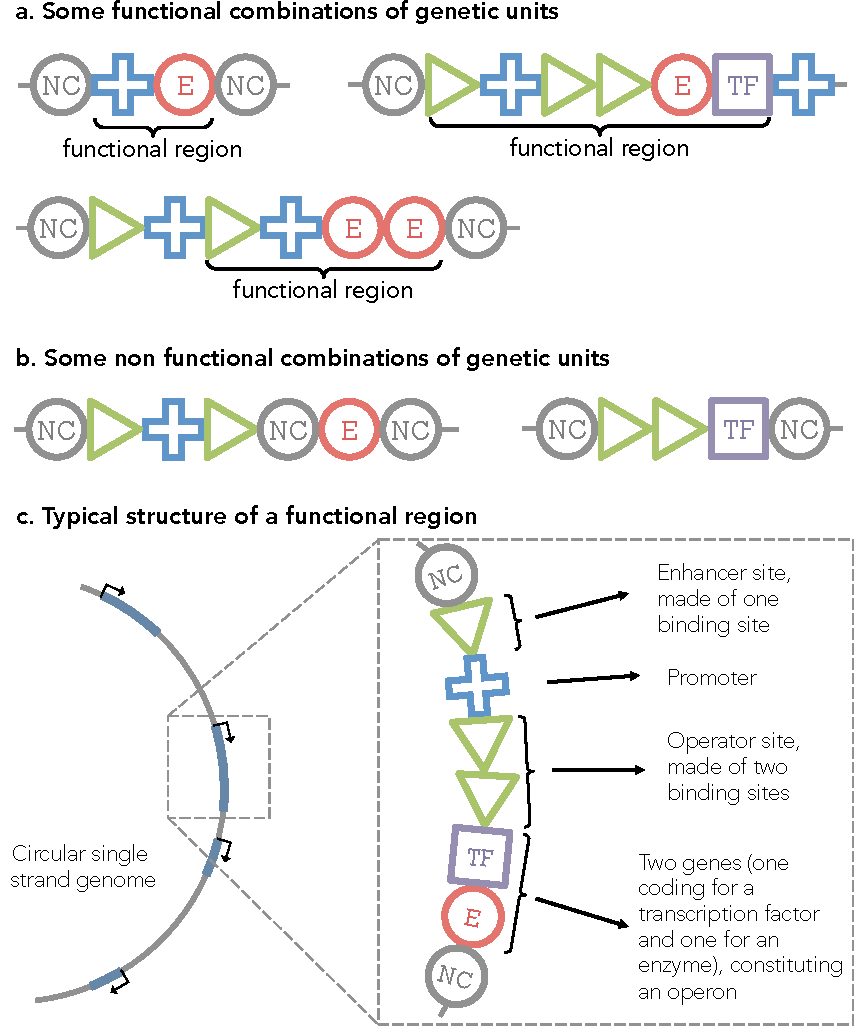
\includegraphics[width=0.8\textwidth]{part2_functional_regions.pdf}
\caption[Some examples of arrangements of genetic units forming functional or non-functional regions.]{\textbf{Some examples of arrangements of genetic units forming or non-functional functional regions.} Grey circles: non-coding units (\textbf{NC}). Blue triangles: binding site units (\textbf{BS}). Orange crosses: promoter units (\textbf{P}). Purple squares: transcription factor coding units (\textbf{TF}). Magenta circles: enzyme coding units (\textbf{E}). The functional regions of a genome are those that have the following pattern: a promoter (\textbf{P}), optionally flanked upstream (enhancer site) or downstream (operator site) by one or more binding sites (\textbf{BS}), followed by one or more contiguous coding units (\textbf{E} or \textbf{TF}). \textbf{a.} Some functional combinations of genetic units. \textbf{b.} Some non functional combinations of genetic units. \textbf{c.} An example of the structure of a typical functional region. The genome is a circular single-strand genome with a single reading frame. A zoom is done in one functional region (magenta regions). The rest of the genome (in grey) is non-coding (non-coding units or any type of unit not correctly arranged to form a functional region).}
\label{fig:part2:methodology:functional_regions}
\end{figure}

%%%%%%%%%%%%%

\subsection{Mutational operators}
\label{subsec:part2:methodology:mutational_operators}

At each replication, the genome undergoes \textbf{point mutations} and \textbf{large rearrangements} (duplications, deletions, translocations and inversions). To account for the effects of these events on the coarse-grained genome, two additional types of mutation have been introduced in {\EvoEvoSim}: \textbf{(i)} \textbf{transitions} : a genetic unit can transit from one type to any other at a certain rate, and \textbf{(ii)} \textbf{breakpoints}: during large rearrangements, genetic units located on sequence breakpoints are exposed to mutations.

\begin{enumerate}
\item[\textbf{(1)}] \textbf{Point mutations.} Point mutations modify the attributes of a genetic unit by adding random values to them. Each attribute (see Table~\ref{table:part2:genetic_units}) owns a dedicated \textbf{mutation kernel} whose properties are predefined as model parameters (usually uniform or gaussian). Two types of attribute exist: integer values and floating-point values. Integer variables mutate by adding a random value from a uniform distribution. Floating-point variables mutate by adding a random value from a normal distribution. For example, the basal expression level $\beta$ (a floating-point variable) mutation kernel is a normal law with a variance defined by the user at the beginning of the simulation. The substrate tag $s$ (an integer value) mutation kernel is a uniform law with a range defined by the user at the beginning of the simulation. In summary, the parameters of eight mutation kernels have to be set by the user (see the {\EvoEvoSim} user guide in Appendix \ref{ch:appendix:user_manual}). Besides the parametrization of the mutation kernels, the \textbf{point mutation rate} must be set by the user. The point mutation rate is expressed per attribute per replication;
\item[\textbf{(2)}] \textbf{Transitions.} Genetic units can also undergo a type transition from any unit type to any other at a rate defined by the user. The transition rate is expressed per genetic unit per replication. All types of genetic units are actually implemented as a tuple containing all possible attributes, like $(\text{unit\_type}, \beta, s, p, k_{cat}, k_{cat}/K_M)$. The unit type tells us which parameters are functionally relevant and the others are free to mutate neutrally. Doing so, digital organisms can explore the neutral fitness landscape and potentially innovate if a non-coding unit is re-functionalized by a type transition (as it the case for pseudogenes);
\item[\textbf{(3)}] \textbf{Duplications.} Large duplications consist in duplicating a random sequence on the genome, and inserting the duplicate at a random location. To select the random sequence to duplicate, two random locations are uniformly drawn in the whole genome. The insertion point is also drawn uniformly (for example, it is possible to insert a duplicate in the duplicated sequence). A duplication implies one breakpoint (Fig. \ref{fig:part2:methodology:large_rearrangements}a). The duplication rate is expressed per genetic unit per replication;
\item[\textbf{(3)}] \textbf{Deletions.} Large deletions consist in deleting a random sequence from the genome, and join the two extremities of the remaining sequence. To select the random sequence to delete, two random locations are uniformly drawn. A deletion implies two breakpoints (Fig. \ref{fig:part2:methodology:large_rearrangements}b). The deletion rate is expressed per genetic unit per replication;
\item[\textbf{(4)}] \textbf{Translocations.} Large translocations consist in moving a random sequence from one genome location to another. To select the random sequence to move, two random locations are uniformly drawn. The insertion point is also drawn uniformly in the whole genome. A translocation implies three breakpoints (Fig. \ref{fig:part2:methodology:large_rearrangements}c). The translocation rate is expressed per genetic unit per replication;
\item[\textbf{(5)}] \textbf{Inversions.} Large inversions consist in reverting a random sequence on the genome. To select the random sequence to revert, two random locations are uniformly drawn in the whole genome. An inversion implies two breakpoints (Fig. \ref{fig:part2:methodology:large_rearrangements}d). The inversion rate is expressed per genetic unit per replication;
\item[\textbf{(6)}] \textbf{Breakpoints.} In real genomes, spontaneous rearrangement breakpoints have no reason to lie exactly between two functional regions and could thus break them. To model that with the coarse-grained genome representation, the content of the two genetic units that are adjacent to a rearrangement breakpoint is altered. Suppose for example that a deletion joins two genetic units, one containing the attributes ($\text{unit\_type}_1$, $\beta_1$, $s_1$, $p_1$, $k_{cat1}$, $(k_{cat}/K_M)_1$) and the other the attributes ($\text{unit\_type}_2$, $\beta_2$, $s_2$, $p_2$, $k_{cat2}$, $(k_{cat}/K_M)_2$). Then for each attribute, there is a probability for the value in unit 1 to be exchanged with the value in unit 2. Both units could for example exchange their values of $s$, thereby leading to ($\text{unit\_type}_1$, $\beta_1$, $s_2$, $p_1$, $k_{cat1}$, $(k_{cat}/K_M)_1$) and ($\text{unit\_type}_2$, $\beta_2$, $s_1$, $p_2$, $k_{cat2}$, $(k_{cat}/K_M)_2$). The breakpoint rate is expressed per breakpoint per replication, and must be set by the user.
\end{enumerate}

\begin{figure}[!h]
\centering 
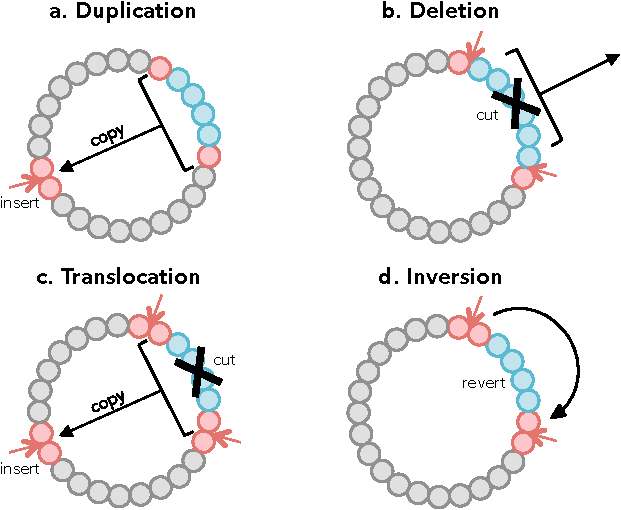
\includegraphics[width=0.8\textwidth]{part2_large_rearrangements.pdf}
\caption[The four types of large rearrangements in {\EvoEvoSim}.]{\textbf{The four types of large rearrangements in {\EvoEvoSim}.} At replication, genomes undergo four types of large rearrangements: \textbf{a.} duplications, \textbf{b.} deletions, \textbf{c.} translocations, and \textbf{d.} inversions. The genome sequence targeted by the rearrangement is colored in blue. Breakpoints are represented by red arrows. The genetic units undergoing mutations at breakpoints are colored in red.}
\label{fig:part2:methodology:large_rearrangements}
\end{figure}

%%%%%%%%%%%%%%%%%%%%%%%%% SECTION : THE GENETIC REGULATORY NETWORK %

\section{The genetic regulatory network}
\label{sec:part2:methodology:grn}

When transcription factors are expressed, they can contribute to the genetic regulatory network by binding to functional enhancer or operator sites. At each time-step $t$ and for each promoter $i$ belonging to a functional region, four steps are necessary to compute the activity of the network:

\begin{enumerate}

% COMPUTE BINDING SITE ACTIVITY
\item[\textbf{(1)}] The activity $A_s(t)$ of each binding site $s$ reads:

\begin{equation}
\label{eq:part2:methodology:binding_site_activity}
A_s(t) = \sum_j c_j(t) A_{js}
\end{equation}

with $c_j(t)$ the concentration of the transcription factor $j$ at time $t$ and $A_{js} \in [0, 1]$ the affinity of this transcription factor for the binding site $s$. In the following, all the concentrations will be expressed in \textbf{arbitrary concentration units} (ACU).
The affinity $A_{js}$ depends on the distance between the transcription factor tag $\text{TF}_\text{tag}(j) \in \mathbb{Z}$ and the binding site tag $\text{BS}_\text{tag}(j) \in \mathbb{Z}$, and the binding window $W_\text{bind}(j)$ of the transcription factor $j$. It reads:

\begin{equation}
\label{eq:part2:methodology:affinity}
A_{js} = \left\{
\begin{array}{l l}
1-\dfrac{|\text{TF}_\text{tag}(j) - \text{BS}_\text{tag}(j)|}{W_\text{bind}(j)} & \text{if \quad $|\text{TF}_\text{tag}(j) - \text{BS}_\text{tag}(j)| \leq W_\text{bind}(j)$}\\\\
0 & \text{else}
\end{array}
\right.
\end{equation}

Figure \ref{fig:part2:methodology:affinity} shows the variation of the affinity when the distance between the transcription factor tag and the binding site tag varies.

\begin{figure}[!ht]
\centering 
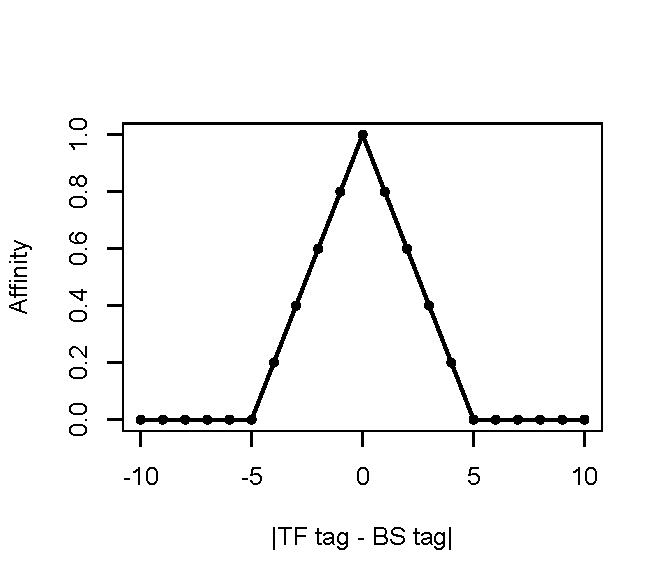
\includegraphics[width=0.5\textwidth]{part2_affinity.pdf}
\caption[The affinity of a transcription factor for a binding site depends on the distance between their respective tags.]{\textbf{The affinity of a transcription factor for a binding site depends on the distance between their respective tags.} On x-axis, the distance between the transcription factor tag and the binding site tag. On y-axis, the affinity computed thanks to Eq~\ref{eq:part2:methodology:affinity}. Here the binding window $W_\text{bind} = 5$.}
\label{fig:part2:methodology:affinity}
\end{figure}

% COMPUTE ENHANCER AND OPERATOR REGIONS ACTIVITY
\item[\textbf{(2)}] From \textbf{(1)}, the activities of the enhancer site $E_i(t) > 0$ and of the operator site $O_i(t) > 0$ flanking the promoter $i$ read:

\begin{equation}
\label{eq:part2:methodology:enhancer_operator_activity}
\left\{
\begin{array}{rcl}
E_i(t) & = & \sum\limits_{s\ \in\ \text{enhancer}_i} A_s(t)\\\\
O_i(t) & = & \sum\limits_{s\ \in\ \text{operator}_i} A_s(t)
\end{array}
\right.
\end{equation}

% COMPUTE THE EXPRESSION RATE
\item[\textbf{(3)}] Then, the expression rate $e_i(t)$ of the promoter $i$ is given by the following Hill-like function:

\begin{equation}
\label{eq:part2:methodology:hill_function}
e_i(t) = \beta_i . \left( \dfrac{\theta^n}{O_i(t)^n + \theta^n} \right) . \left( 1 + \left( \dfrac{1}{\beta_i} - 1 \right) . \left( \dfrac{E_i(t)^n}{E_i(t)^n + \theta^n} \right) \right)
\end{equation}

with $\beta_i \in [0, 1]$ the basal expression level of the promoter $i$, $n$ and $\theta$ two constants shaping the Hill-like function (defined by the user).

% COMPUTE THE EVOLUTION OF PROTEIN CONCENTRATIONS
\item[\textbf{(4)}] At each time-step $t$, coding units being controlled by the promoter $i$ are expressed at a rate $e_i(t)$. Then, the concentration of each protein depending on the promoter $i$ in the cytoplasm depends on the following synthesis-degradation rule:

\begin{equation}
\left\{
\begin{array}{l}
c_i(0) = \dfrac{\beta_i}{\phi}\\\\
\dfrac{\partial c_i}{\partial t} = e_i(t) - \phi . c_i(t)
\end{array}
\right.
\end{equation}

with $\phi$ the protein degradation rate, set by the user before the beginning of any simulation.

\end{enumerate}

%%%%%%%%%%%%%%%%%%%%%%%%% SECTION : THE METABOLIC NETWORK %

\section{The metabolic network}
\label{sec:part2:methodology:metabolism}

Enzyme coding units products can either be pumps, pumping metabolites from or to the growth medium, or enzymes performing catalytic transformations in the metabolic space.
 
Let us consider an enzyme in the cytoplasm that catalyzes one specific reaction $s \rightarrow p$ (with $s \in \mathbb{N}^*$ and $p \in \mathbb{N}^*$ being the substrate and the product of a Michaelis-Menten-like reaction, respectively). The variation in concentrations $[s]$ and $[p]$ over time are then driven by Eq~\ref{eq:michaelis_menten}:

\begin{eqnarray}
\label{eq:michaelis_menten}
\left\{
\begin{array}{lcr}
\dfrac{d[s]}{dt} = -\dfrac{k_{cat}[E][s]}{K_M+[s]}\\\\
\dfrac{d[p]}{dt} = \dfrac{k_{cat}[E][s]}{K_M+[s]}
\end{array}
\right.
\end{eqnarray}

where $K_M$ and $k_{cat}$ are the kinetic attributes of the enzyme ($K_M$ being deduced from $k_{cat}$ and $k_{cat}/K_M$ attributes).

Is $s=p$, enzymes are treated as pumps, for which $[s]$ and $[p]$ describe the internal and external concentrations of the same metabolite. If $k_{cat}$ is positive (resp. negative), $[s]$ is the external (resp. internal) concentration of the metabolite and $[p]$ the internal (resp. external) concentration. The dynamics of metabolic concentrations $[s]$ and $[p]$ are thus also driven by Eq~\ref{eq:michaelis_menten} when the enzyme coding unit product is a pump.

%%%%%%%%%%%%%%%%%%%%%%%%% SECTION : COUPLING NETWORKS %

\section{Coupling the genetic regulatory network and the metabolic network}
\label{sec:part2:methodology:coupling_networks}

Bacteria are able to sense their environment by detecting the presence of a particular molecule or signal, and to give an appropriate answer by updating their gene expression profile. The archetype of this behaviour is the \textbf{lactose operon} \citep{jacob-and-monod-1961}.

As shown in Figure \ref{fig:part2:methodology:lactose_operon}, this operon is composed of three genes (\textit{lacZ}, \textit{lacY} and \textit{lacA}), controlled by one promoter flanked by an operator. Another gene, \textit{lacI}, codes for a transcription factor which inhibates the operon when binding on the operator. \textit{lacI} is constitutively expressed and its concentration in the cytoplasm is almost constant. However its conformation, hence its affinity for the operator is modified by lactose. In absence of lactose, \textit{lacI} is active and down-regulates the operon. If lactose is present, it binds on \textit{lacI} and inhibits it. In this case, the operon is expressed and the cell is able to degrade lactose.

This mechanism is integrated to {\EvoEvoSim}: some metabolites can behave as co-enzymes, and repress or activate transcription factors activity. To this aim, each transcription factor own a co-enzyme tag $\text{CoE}_\text{tag} \in \mathbb{N}^*$, a co-enzyme constant $k_\text{CoE}$, a free activity $A_{\text{free}}$ and a bound activity $A_{\text{bound}}$. A metabolite $m$ can repress or activate a transcription factor in four ways:
\begin{enumerate}
\item[\textbf{(1)}] If $A_{\text{free}} = 1$ and $A_{\text{bound}} = 0$, $m$ inhibits the transcription factor;
\item[\textbf{(2)}] If $A_{\text{free}} = 0$ and $A_{\text{bound}} = 1$, $m$ activates the transcription factor;
\item[\textbf{(3)}] If $A_{\text{free}} = 1$ and $A_{\text{bound}} = 1$, the transcription factor is always activated;
\item[\textbf{(4)}] If $A_{\text{free}} = 0$ and $A_{\text{bound}} = 0$, the transcription factor is always repressed.
\end{enumerate}

\begin{figure}[!h]
\centering 
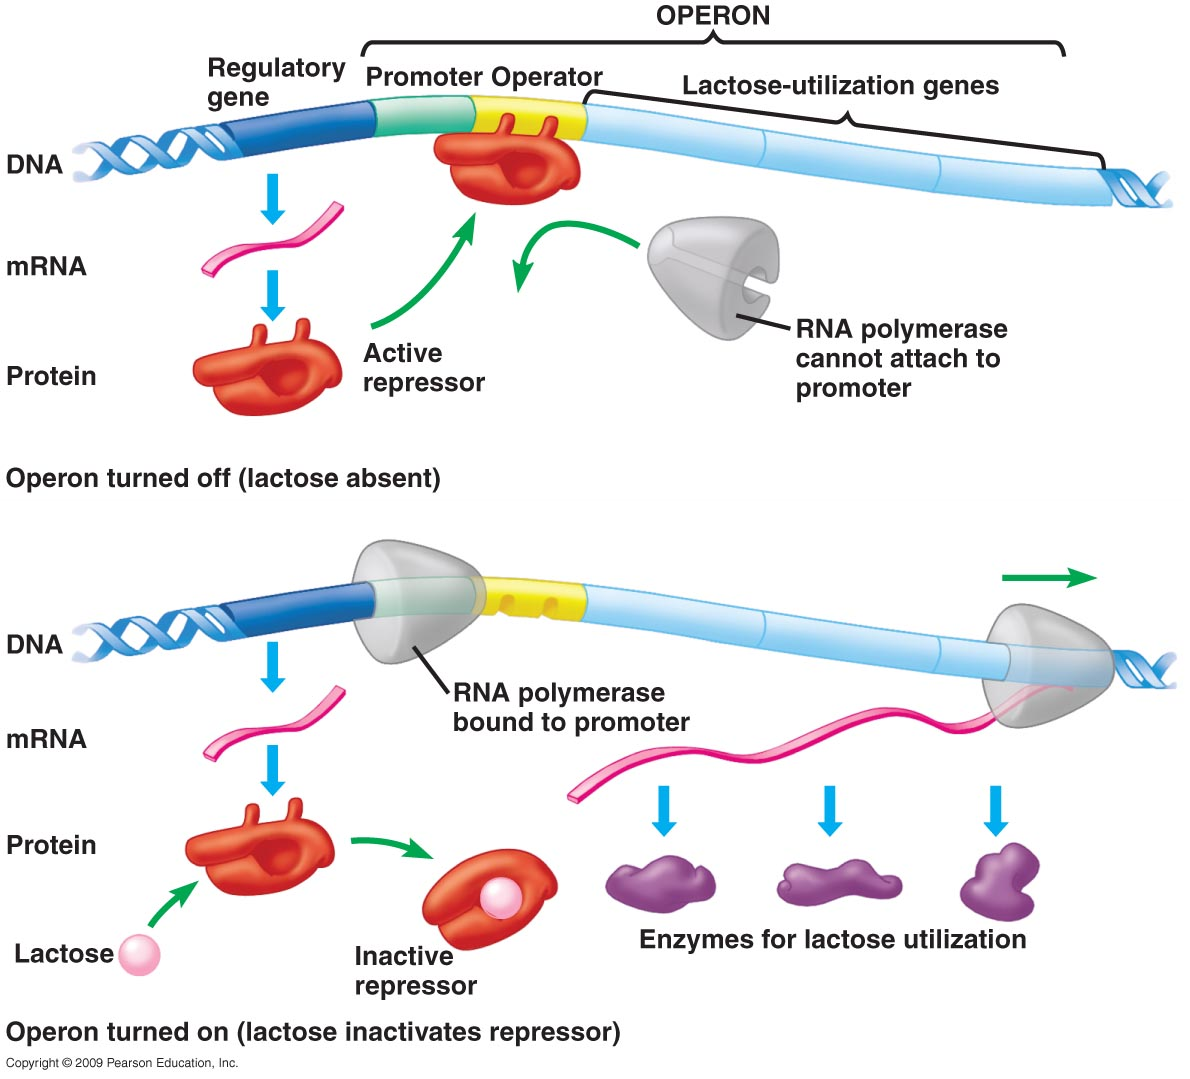
\includegraphics[width=0.8\textwidth]{part2_lactose_operon.jpg}
\caption[The lactose operon.]{\textbf{The lactose operon.} The lactose operon is inactive in the absence of lactose (top) because a repressor blocks attachment of RNA polymerase to the promoter. With lactose present (bottom), the repressor is inactivated, and transcription of lactose-processing genes proceeds (from \href{https://2fsfox.blogspot.fr/2013/05/the-lac-operon-continued-and-other.html}{https://2fsfox.blogspot.fr/2013/05/the-lac-operon-continued-and-other.html}).}
\label{fig:part2:methodology:lactose_operon}
\end{figure}

Table~\ref{table:part2:co_enzyme_activity} resumes these different outcomes by using the following picture: let's consider a transcription factor as a structure with two arms, linked by a pivotal point. The active site of the transcription factor is located on one arm, its exposure depending on the equilibrium state (or conformation) of the structure. Two configurations are possible: one when the transcription factor is free, and another when a co-enzyme binds to it via the anchoring points located at arms end. The combination of free and bound activities then leads to four behaviors, as described in Equation \ref{eq:part2:methodology:co_enzyme_activity}.

\begin{equation}
[\text{TF}_+] = 
\left\{
\begin{array}{ccl}
\left[\text{TF}\right] \times \dfrac{k_\text{CoE}}{k_\text{CoE}+[m]} & \text{ if } & A_{free}=1 \text{ and } A_{bound}=0\\\\
\left[\text{TF}\right] \times \dfrac{[m]}{k_\text{CoE}+[m]} & \text{ if } & A_{free}=0 \text{ and } A_{bound}=1\\\\
\left[\text{TF}\right] & \text{ if } & A_{free}=1 \text{ and } A_{bound}=1\\\\
0.0 & \text{ if } & A_{free}=0 \text{ and } A_{bound}=0
\end{array}
\right.
\label{eq:part2:methodology:co_enzyme_activity}
\end{equation}


\begin{tablehere}
\begin{adjustwidth}{0in}{0in}
\centering
\caption[The eight possible states of a transcription factor.]{\textbf{The eight possible states of a transcription factor.} The transcription factor is represented in dark grey. Its active site (the part allowing binding on a binding site) is represented in green. Depending on free and bound activities attributes, the co-enzyme (in blue) acts as an activator or a repressor. The active site is then free (or not) to bind on a binding site.}
\begin{tabular}{ | c | c | c | c |}
\hline
\textbf{Free TF} & \textbf{Bound TF} & \textbf{Free activity} & \textbf{Bound activity}\\
\hline

\begin{minipage}{3cm}
\centering

\includegraphics{TF1.pdf}
\end{minipage}
& 
\begin{minipage}{3cm}
\centering

\includegraphics{TF2.pdf}
\end{minipage}
&
\textit{1}
&
\textit{0}
\\
\hline

\begin{minipage}{3cm}
\centering

\includegraphics{TF3.pdf}
\end{minipage}
& 
\begin{minipage}{3cm}
\centering

\includegraphics{TF4.pdf}
\end{minipage}
&
\textit{0}
&
\textit{1}
\\
\hline

\begin{minipage}{3cm}
\centering

\includegraphics{TF5.pdf}
\end{minipage}
& 
\begin{minipage}{3cm}
\centering

\includegraphics{TF6.pdf}
\end{minipage}
&
\textit{1}
&
\textit{1}
\\
\hline

\begin{minipage}{3cm}
\centering

\includegraphics{TF7.pdf}
\end{minipage}
& 
\begin{minipage}{3cm}
\centering

\includegraphics{TF8.pdf}
\end{minipage}
&
\textit{0}
&
\textit{0}
\\
\hline

\end{tabular}
\begin{flushleft}

\end{flushleft}
\label{table:part2:co_enzyme_activity}
\end{adjustwidth}
\end{tablehere}




%%%%%%%%%%%%%%%%%%%%%%%%% SECTION : ENERGY CONSTRAINTS %

\section{Optional feature: energy constraints}
\label{sec:part2:methodology:energy_constraints}

One of the most evident constraints living organisms must cope with in the real world are the laws of thermodynamics. Indeed, real organisms cannot violate the energy balance with their environment, or have negative entropy. One direct consequence is that global entropy cannot decrease, whatever the organism's activity. For example, catabolic reactions produce heat, that will propagate in the local environment of the organism (and possibly kill it). This energy is lost for the organism.
In this sense, life could be seen as a fight against entropy \citep{alberts-et-al-2013}, as illustrated in Figure \ref{fig:part2:methodology:desk_entropy}.
Billions years of evolution made cells very efficient engines to exploit the energy gained with catabolism. Energy carriers, like ATP molecules, allow cells to transfer the energy won by degrading food, or capturing photons, in useful but costly reactions (for example, producing---or actively degrading---a protein). This coupling between food process (catabolism), and production of useful macromolecules (anabolism) is at the heart of cell's metabolism.

We introduced energy constraints in {\EvoEvoSim} by doing the distinction between two types of reactions: reactions rewarding the cell in energy (catabolic reactions), and reactions consuming energy (anabolic reactions). Implicit energy carrier molecules allow us to compute the \textbf{energy balance} $\mathcal{E}$ of the cell at each time-step $t$. To this aim, we introduced a notion of reaction cost, each type of reaction owning a specific cost defined by the user before the beginning of a simulation. There are four energy costs:
\begin{enumerate}
\item[\textbf{(1)}] The \textbf{expression cost} $c_{\text{expr}} \geq 0$: the cell consumes energy when proteins are expressed;
\item[\textbf{(2)}] The \textbf{degradation cost} $c_{\text{degr}} \geq 0$: the cell consumes energy when proteins are degraded (symbolizing, \textit{e.g.}, the functioning of the proteasome);
\item[\textbf{(3)}] The \textbf{enzymatic cost} $c_{\text{enz}} \geq 0$: depending on the type of metabolic reaction (see below), the cell consumes or produces energy when an enzymatic reaction is performed;
\item[\textbf{(4)}] The \textbf{pumping cost} $c_{\text{pump}} \geq 0$: the cell consumes energy when a metabolite is pumped in or out;
\end{enumerate}

\begin{figure}[!h]
\centering 
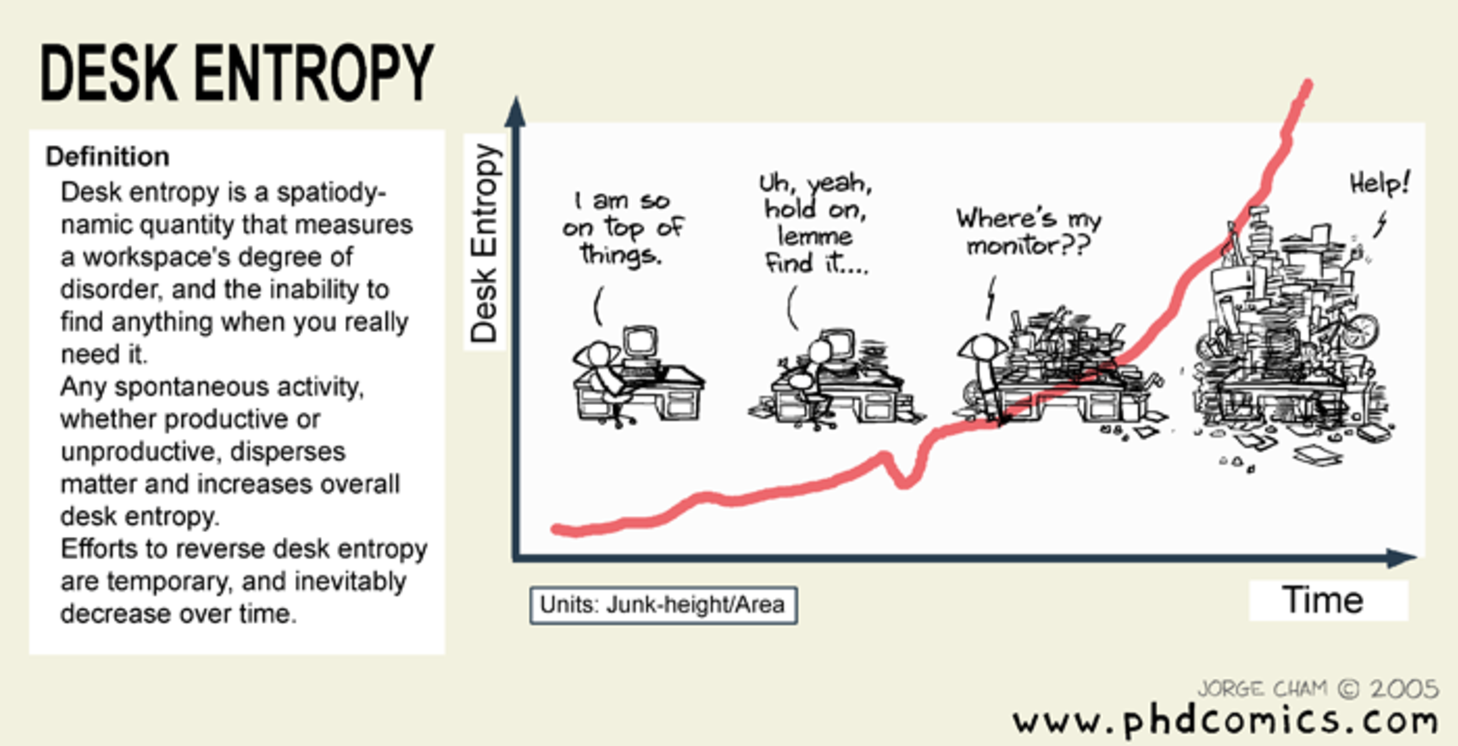
\includegraphics[width=1\textwidth]{part2_deskentropy.pdf}
\caption[An impossible-to-win fight against entropy.]{\textbf{An impossible-to-win fight against entropy.} An illustration of the unavoidable increase of entropy in a system (from \href{www.phdcomics.com}{www.phdcomics.com}).}
\label{fig:part2:methodology:desk_entropy}
\end{figure}

Enzymatic reactions consume or produce energy depending on the values of the substrate tag $s$, the product tag $p$ and the enzymatic cost $c_{\text{enz}}$:
\begin{enumerate}
\item[\textbf{(1)}] if $s < p$, the reaction consumes energy at a rate $(p-s) . c_{\text{enz}}$
\item[\textbf{(2)}] if $s > p$, the reaction produces energy at a rate $(s-p) . c_{\text{enz}}$
\end{enumerate}

It is then possible to describe the evolution of the energy balance $\mathcal{E}$ through time, as following:

\begin{equation}
\label{eq:part2:methodology:energy_balance}
\left.
\begin{array}{rcl}
\dfrac{\partial \mathcal{E}}{\partial t} & = & \sum\limits_{i\ \in\ \text{catabolic reactions}} \left( \dfrac{\partial [p_i]}{\partial t} \times (s_i - p_i) \times c_{\text{enz}} \right)\\\\
& - & \sum\limits_{i\ \in\ \text{anabolic reactions}} \left( \dfrac{\partial [p_i]}{\partial t} \times (p_i - s_i) \times c_{\text{enz}} \right)\\\\
& - & \sum\limits_{i\ \in\ \text{inflowing pumps}} \left( \dfrac{\partial [s_{in}]}{\partial t} \times (s_{in} - s_{out}) \times c_{\text{pump}} \right)\\\\
& - & \sum\limits_{i\ \in\ \text{outflowing pumps}} \left( \dfrac{\partial [s_{out}]}{\partial t} \times (s_{out} - s_{in}) \times c_{\text{pump}} \right)\\\\
& - & \sum\limits_{i\ \in\ \text{expressed genes}} \left( \dfrac{\partial [e_i]}{\partial t} \times c_{\text{expr}} \right)\\\\
& - & \sum\limits_{i\ \in\ \text{degraded proteins}} \left( [c_i] \times \phi \times c_{\text{degr}} \right)
\end{array}
\right.
\end{equation}

For practical reasons, $\mathcal{E}$ is not solved as an ordinary differential equation. Indeed, incorporating energy in differential equations would have lead to intractable simulations. For this reason, the energy balance $\mathcal{E}$ is evaluated at the end of each simulation time-step $t$. The cell's score is impaired if the energy balance $\mathcal{E} \leq 0$ (the score function is described below).

%%%%%%%%%%%%%%%%%%%%%%%%% SECTION : THE SCORE FUNCTION %

\section{The score function}
\label{sec:part2:methodology:score_function}

The set of all metabolites contained in the cell's cytoplasm can be converted into a unique concentration vector $\boldsymbol{M} = \{m_1, m_2, ..., m_n\}$. In {\EvoEvoSim}, $\boldsymbol{M}$ constitutes the ``phenotype'' determining the score $S$ of the cell. It is then possible to define a score function $f : \mathbb{R}^n \rightarrow \mathbb{R}_+$ such that $S = f(\boldsymbol{M})$.

Some metabolites are essential to cell's growth, and some other are intermediate products or waste. In {\EvoEvoSim}, essential metabolites are \textbf{prime numbers}: their production contributes to the growth rate by increasing the probability to produce offspring. However, producing metabolites above a predefined threshold leads to cell's toxicity, and impairs cell's score. Let's define the subset of $\boldsymbol{M}$ representing the essential metabolites $\boldsymbol{E} = \{e_1, e_2, ..., e_m\} \subset \boldsymbol{M}$. Then, the score $S$ of the cell is:
\begin{equation}
S = 
\left\{
\begin{array}{lcr}
\sum_i e_i & \mbox{if} & (\forall e \in \boldsymbol{E}\  |\ e < T_E) \cup  (\forall m \in (\boldsymbol{M} \backslash \boldsymbol{E})\  |\ m < T_M)\\\\
0 & \mbox{else} &
\end{array}
\right.
\end{equation}
with $T_M$ the toxicity threshold of non-essential metabolites ($\boldsymbol{M} \backslash \boldsymbol{E})$ and $T_E$ the toxicity threshold of essential metabolites ($\boldsymbol{E}$).

If the cell's score is under a minimum score $S < S_{\text{min}}$ defined by the user, then $S = 0$.

Importantly, the score and the fitness are different. The score represents the instantaneous performance of a cell (being computed at each time-step), while the fitness is usually defined as the combined effect of survival and reproduction, and can only be computed \textit{a posteriori}, when the whole cell's history is known. We will never compute the fitness in {\EvoEvoSim}. Instead, we will analyze the lineage of the final population, that is supposed to have increased its mean fitness through time, in order to recover evolutionary events.

%%%%%%%%%%%%%%%%%%%%%%%%% SECTION : POPULATION AND SELECTION %

\section{Population and selection}
\label{sec:part2:methodology:population_selection}

Organisms evolve on a two-dimensional toroidal grid (each location containing at most one organism), and compete for the external metabolites to produce offspring in empty locations. They interact with their local environment by pumping metabolites in and out and they release their metabolic content at death. At each time-step, organisms are evaluated and either killed, updated or replicated depending on their current state:
\begin{enumerate}
\item[\textbf{(1)}] If the organism does not die and cannot divide (\textit{e.g.}, because there is no free space in its neighborhood), its metabolic network is updated, and its score is computed;
\item[\textbf{(2)}] Organisms can also die randomly with a probability following a Poisson law of parameter $p_{death}$ expressed per organism per time-step. At death, the metabolic content of a cell is released into the local environment;
\item[\textbf{(3)}] For each empty grid location, all living organisms in the Moore neighborhood whose score is higher than a minimum score $S_{min}$ compete. The organism having the best score in the neighborhood is allowed to divide if it did not replicate previously at the same time-step (such that any dividing cell generates at most two daughters per time-step).
\end{enumerate}

%%%%%%%%%%%%%%%%%%%%%%%%% SECTION : ENVIRONMENT %

\section{The environment}
\label{sec:part2:methodology:environment}

The physical environment is described at the grid level: each grid location contains external metabolites, each with its concentration.
These external metabolites diffuse with a diffusion parameter $D$ expressed in gridstep\textsuperscript{2}.time-step\textsuperscript{-1}, meaning that a fraction $D$ of each metabolite present at one location will diffuse to each of the eight neighboring grid locations at each time-step. The discrete diffusion equation we are using is inspired from \cite{frenoy-et-al-2013}. External metabolites are also degraded with a degradation rate $D_g$, meaning that a fraction $D_g$ of each metabolite at each location will disappear at each time-step. We made the simplifying assumption that there are no enzymatic reaction in the environment, and that metabolite transformation only occurs inside the organisms.

At each time-step $t$, each grid location $k$ of coordinates $(x,y)$ is characterized by the individual occupying the location (possibly none), and the list of free metabolites, each metabolite $i$ being at concentration $c_{i,k}(t)$. Given the parameters of the environment, the dynamics of a free metabolite $i$ in a grid location $k$ reads:
\begin{equation}
\label{eq:part2:methodology:environment}
c_{i,k}(t+1) = c_{i,k}(t) - D_g . c_{i,k}(t) + \sum_{j\ \in\ \text{neighbors}} D . c_{i,j}(t) - 8 . D . c_{i,k}(t) + I_i(t)
\end{equation}
With $I_i$ the inflow rate of metabolite $i$ in the environment.

In conclusion, {\EvoEvoSim} allows for a precise parametrization of the environment. Apart from parameters described above, it is possible for the user to set a variety of behaviors (\textit{e.g.} the periodicity of metabolites influx, the type of metabolites provided or their locations, ...). It is thus possible to mimic realistic experimental setups, such as chemostat or batch-culture, as we will discuss in the next chapter.

%%%%%%%%%%%%%%%%%%%%%%%%% SECTION : TROPHIC NETWORKS %

\section{Trophic networks}
\label{sec:part2:methodology:trophic_networks}

Cells uptake various metabolites, provided externally or being by-products released by other cells. {\EvoEvoSim} keeps trace of the metabolic activity of every cells and computes, at each time-step, a \textbf{trophic network} representing the relationships between cells. This feature is mandatory to study, for example, the evolution of cross-feeding in the population. 

At each time-step $t$, a \textbf{trophic profile} is computed for each organism from its metabolic network activity. The trophic profile is a bit string summarizing the uptake, production, and release activity of an organism. The length of the bit string is defined by the largest metabolite tag present in the system at time $t$. For example, if an organism uptakes metabolite $\#4$, produces $\#3$ from $\#4$ and releases $\#3$, knowing that the largest metabolite tag in the system is $\#5$, then its profile is $|00010|00100|00100|$. Organisms with identical trophic profiles are grouped together, and the trophic network is computed depending on profile relationships. For example, if organisms of a profile $i$ uptake a metabolite produced by a profile $j$, then a directed link is created from $i$ to $j$. Cooperating links are also computed: a cell cooperates with another cell if the former \textbf{actively} releases metabolites useful to the latter.

Trophic profiles are then classified in four \textbf{trophic levels}:
\begin{enumerate}
\item[\textbf{(1)}] \textbf{Level 0} cells exclusively feed on exogenous metabolites, flowing in the environment;
\item[\textbf{(2)}] \textbf{Level 1} cells feed on exogenous metabolites and on metabolites produced by other cells;
\item[\textbf{(3)}] \textbf{Level 2} cells exclusively feed on metabolites produced by other cells;
\item[\textbf{(4)}] \textbf{No level} cells have no active uptaking functions.
\end{enumerate}

Figure \ref{fig:part2:methodology:trophic_network} shows a simple example of trophic network computed on the fly during a simulation, and available in {\EvoEvoSim} HTML viewer (see Appendix \ref{ch:appendix:user_manual}). Exogenously provided metabolites are symbolized by a black node (the \texttt{ENV} node), and other trophic profile nodes are colored depending on their level (purple for level 0, blue for level 1, green for level 2 and grey for no level). Trophic links are represented by solid arrows, cooperating links being represented by dashed arrows.

\begin{figurehere}
\centering 
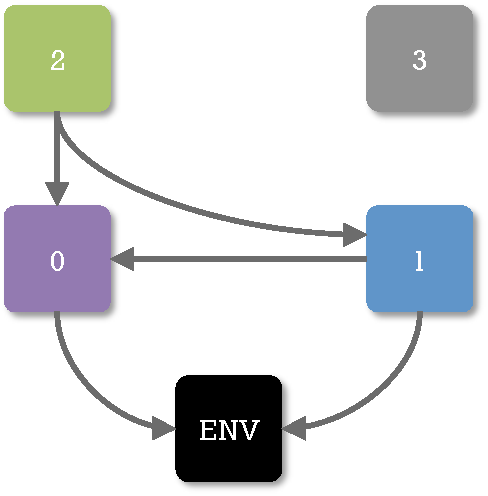
\includegraphics[width=0.3\textwidth]{part2_trophic_network.pdf}
\caption[A basic example of trophic network.]{\textbf{A basic example of trophic network.} A basic example of a trophic network, as it is computed in {\EvoEvoSim}, is presented here. Exogenously provided metabolites are represented by a black node tagged \texttt{ENV}. Trophic profiles (\textit{i.e.}, a group of cells having the exact same metabolic activity) exclusively feeding on exogenous metabolites belong to the level 0, and are represented by purple nodes. Trophic profiles feeding on exogenous metabolites and on by-products of other cells belong to level 1 ; they are represented by blue nodes. Trophic profiles exclusively feeding on by-products are represented by green nodes (level 2). Trophic profiles having no metabolic activity are represented by grey nodes. Here, one level 0 profile feeds on the environment, one level 1 profile feeds on the environment and on profile 0, one level 2 profile feeds on profiles 0 and 1, and one profile has no metabolic activity (no level).}
\label{fig:part2:methodology:trophic_network}
\end{figurehere}

%%%%%%%%%%%%%%%%%%%%%%%%% SECTION : PHYLOGENY %

\begin{figure}[!h]
\centering 
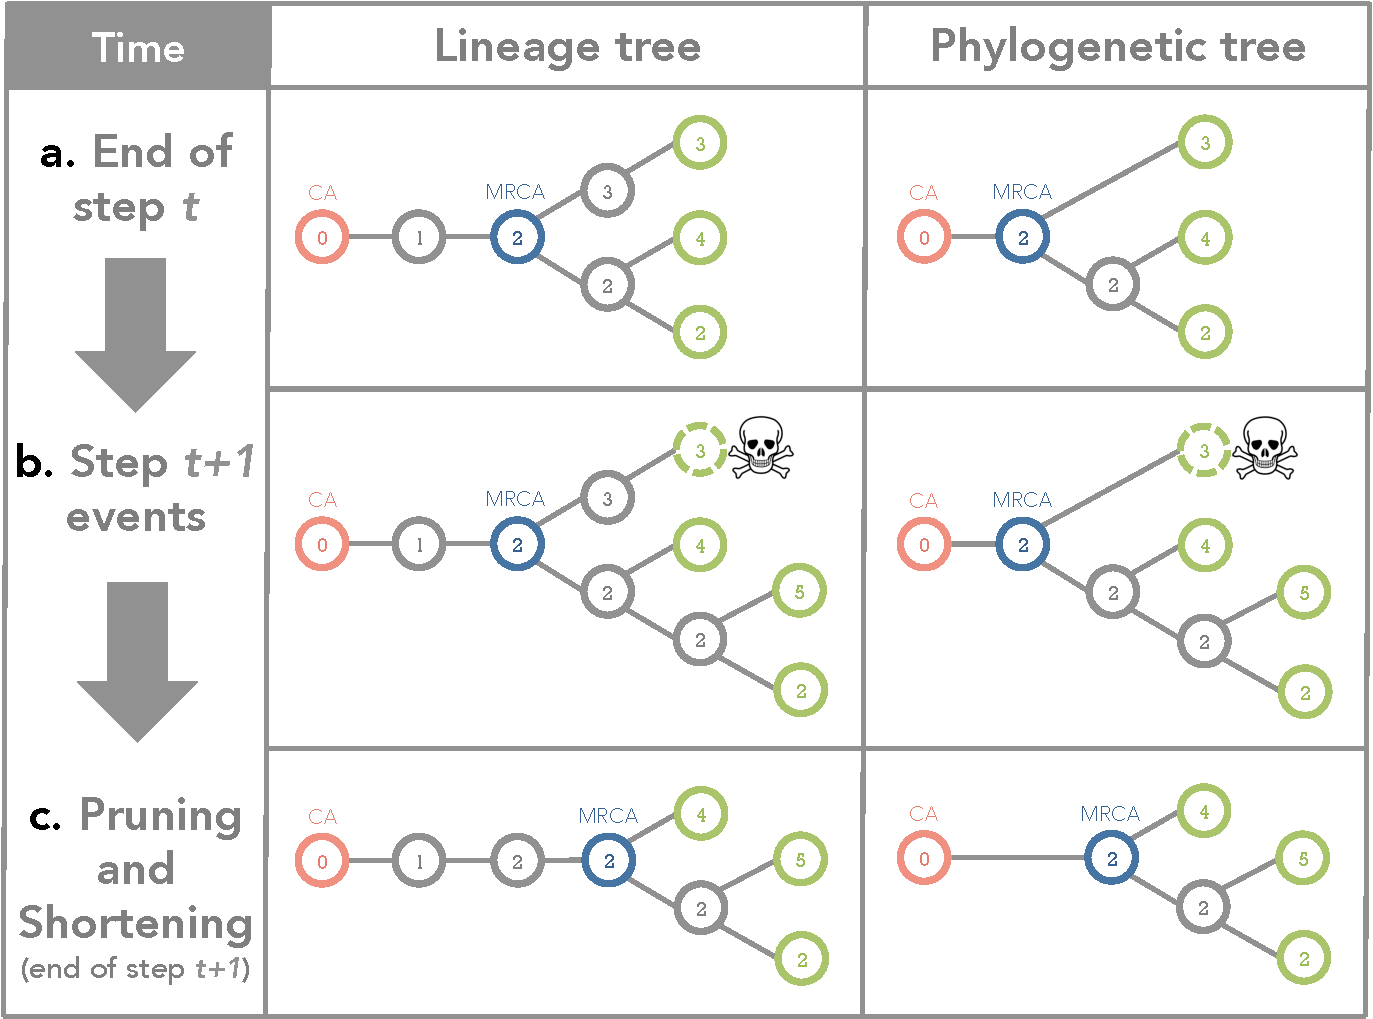
\includegraphics[width=1\textwidth]{part2_trees.pdf}
\caption[Live update of lineage and phylogenetic trees.]{\textbf{Live update of lineage and phylogenetic trees.} At each time-step $t$, the population state is updated (divisions, deaths, cell updates, ...): \textbf{(i)} at each division, the two daughter cells are added to the trees as leaves, with their parent as a common ancestor, \textbf{(ii)} dead cells are removed from trees. Both lineage and phylogenetic trees are pruned (dead branches are removed), and the phylogenetic tree is shortened (intermediate nodes not being common ancestors are removed). \textbf{In this example}, we start at time $t$. The common ancestor of the whole population (\textbf{CA}, in red) is the \textbf{dead cell} labelled $0$. The most recent common ancestor (\textbf{MRCA}, in blue) is the \textbf{alive cell} $2$. Tree leaves are represented in green and all correspond to alive cells (first row). The population state is then updated to time $t+1$: the cell $3$ dies, and the cell $2$ divides in daughter cells $2$ and $5$ (the cell $2$ is still tracked because it divided 4 times and didn't died yet). These events are added to both trees (second row). Then, \textbf{pruning} and \textbf{shortening} algorithms are applied: the lineage tree looses the branch $3-3$. The phylogenetic tree looses the leaf $3$, and the oldest $2$ node. The MRCA is now the node $2$, linked to nodes $2$ and $4$.}
\label{fig:part2:methodology:trees}
\end{figure}

\section{Lineages and phylogeny}
\label{subsec:part2:methodology:phylogeny}

In {\EvoEvoSim}, phylogenetic relationships are exhaustively recorded during a simulation. Two trees are updated at each time-step: the \textbf{lineage tree}, that saves the lineage relationships of every living cells, and the \textbf{phylogenetic tree}, that saves the complete phylogeny of every living cells. Besides phylogenetic relationships, many informations about the genome structure, the phenotype, the mutations, the trophic profile, and so on, are saved in every nodes of the trees. Thus, it is possible to precisely recover the evolution of a population, including fixed mutations. In particular, it is possible to determine if trophic groups are \textbf{monophyletic}, and thus can be considered as \textbf{ecotypes} (see the next chapter for a precise example).

Algorithmically speaking, the phylogenetic tracking deployed in {\EvoEvoSim} is updated as follows: at each simulation time-step $t$, \textbf{(i)} new offspring are added to both trees (Fig. \ref{fig:part2:methodology:trees}b), \textbf{(ii)} both trees are pruned to remove dead branches (Fig. \ref{fig:part2:methodology:trees}c), and \textbf{(iii)} the phylogenetic tree is shortened to remove intermediate nodes between common ancestors (Fig. \ref{fig:part2:methodology:trees}c). One node in the lineage or phylogenetic tree corresponds to one generation in the population. This means that when a cell produces offspring, new nodes are created for the two daughters, even if each cell is individually tracked for its entire life. For example, two or more contiguous nodes in a tree could correspond to a single cell that divided one or more times, as shown in Figure \ref{fig:part2:methodology:trees} with cell $\#2$. In each tree, the common ancestor (CA) of the whole population is tagged (red node on Fig. \ref{fig:part2:methodology:trees}), as well as the most recent common ancestor (MRCA, blue node on Fig. \ref{fig:part2:methodology:trees}).

%%%%%%%%%%%%%%%%%%%%%%%%% SECTION : GENERAL ALGORITHM %

\section{General algorithm}
\label{sec:part2:methodology:general_algorithm}

The general algorithm behind {\EvoEvoSim} is a classical, asynchronous algorithm of \textit{in silico} evolution \citep{hindre-et-al-2012}. At each time-step, each living cell is evaluated, and a decision is made between death, division, or simple update (as presented in Fig.~\ref{fig:part2:methodology:general_algorithm}). The lineage and phylogenetic trees are updated on the fly, as well as the trophic network. In the same time, very complete statistics are computed (tracking hundred of variables), and a large amount of statistics (population means, best individual lineage, phylogeny, ...) are displayed on the fly, in the {\EvoEvoSim} HTML viewer (see Appendix \ref{ch:appendix:user_manual}).

To solve the ordinary differential equations, We used the adaptive Runge-Kutta-Cash-Karp method (RKCK). At each simulation time-step $t$ and for each alive cell, the state of the genetic regulatory network and the metabolic network are updated by solving the ODE system during $t_{\text{ODE}}$ time-steps. This constant is set by the user before the beginning of the simulation (usually $t_{\text{ODE}} = 100$, meaning that each simulation time-step corresponds to 100 ODE time-steps). Altogether, if we consider a $32 \times 32$ environmental grid full of organisms, a time-step involves a thousand of ODE systems. The parameter values of each ODE system are potentially unique, as they are encoded in the organism's genome and thus result from the mutation process. Those ODE systems can also differ by their number of equations, which depends on the organism's genome.

Moreover, {\EvoEvoSim} admits parallel computing algorithms, and is designed for high performance computing (see the user guide in Appendix \ref{ch:appendix:user_manual}).

\newpage
\begin{figurehere}
\centering 
\includegraphics[width=1\textwidth]{part2_general_algorithm.pdf}
\caption[Global picture of {\EvoEvoSim}.]{\textbf{Global picture of {\EvoEvoSim}.} \textbf{a. Description of the genotype-to-phenotype mapping.} Organisms own a coarse-grained genome made of units. This genome is a circular single-strand sequence, with a unique reading frame. Non coding \textbf{(NC)} units are not functional \textbf{(a.1)}. The arrangement of the units on the sequence defines functional regions, where a promoter (\textbf{P}, blue cross) controls the expression of enzyme coding units (\textbf{E}, red circles) or transcription factor coding units (\textbf{TF}, purple squares), thereby allowing for operons (here, one E and one TF). When coding units are expressed \textbf{(a.2)}, they contribute to the genetic regulatory network (for TFs) and the metabolic network (for Es).
Depending on their attributes (see~\ref{sec:part2:methodology:genome} and~\ref{sec:part2:methodology:grn}), transcription factors bind on binding sites. \textbf{(a.3)} If they bind on the enhancer sequence (binding sites flanking the promoter upstream), the promoter activity is up-regulated. If they bind on the operator sequence (binding sites flanking the promoter downstream), the promoter activity is down-regulated. \textbf{(a.4)} Metabolites can bind on a transcription factor as co-enzymes, and activate or inhibit it, depending on transcription factor attributes (see~\ref{sec:part2:methodology:coupling_networks}).
Enzymes perform metabolic reactions in the cytoplasm \textbf{(a.5)}, or pump metabolites in or out \textbf{(a.6)}. The score of an organism is computed from its ``essential metabolites''
(usually the score is the sum of essential metabolite concentrations). Lethal toxicity thresholds are applied to each metabolic concentration and forbid organisms to accumulate resources. \textbf{b. Description of the population and environment levels.} Organisms are placed on a 2D toroidal grid, and compete for resources and space. When an organism dies, it leaves its grid cell empty and organisms in the Moore neighborhood (if any) compete to divide in available space. The competition is based on scores, a minimal threshold being applied on scores to forbid worst organisms to divide. At division, daughters share cytoplasm content (enzymes and metabolites). At death, metabolites from the cytoplasm are released in the local environment, and diffuse on the grid \textbf{(b.1)}. On the largest scale, the population evolves on the environment by up-taking, transforming and releasing metabolites. Metabolites then diffuse and are degraded. This strong interaction between the population and the environment allows for the evolution of complex ecological situations, depending on environmental properties \textbf{(b.2)}.}
\label{fig:part2:methodology:general_algorithm}
\end{figurehere}

%%%%%%%%%%%%%%%%%%%%%%%%% SECTION : CODE AVAILABILITY %

\section{Code availability}
\label{sec:part2:methodology:code_availability}

We developed {\EvoEvoSim} in C++, from scratch. Some scripts are written in Python and R, especially for the automatic generation of live statistics and figures. We also implemented a HTML viewer, including many informations (from best lineage evolution to phylogeny), useful to track evolution during a simulation. This viewer includes some Javascript. The code is hosted on Github in \texttt{charlesrocabert/Evo2Sim} repository. The {\EvoEvoSim} user manual is available in Appendix \ref{ch:appendix:user_manual}. Some simulation examples are also available on the EvoEvo project website at \href{http://evoevo.liris.cnrs.fr/evo2sim/}{http://evoevo.liris.cnrs.fr/evo2sim/}.

%%%%%%%%%%%%%%%%%%%%%%%%% SECTION : WHAT NEXT ? %

\section{What next?}
\label{sec:part2:methodology:what_next}

In the two following chapters, we will present two results obtained with {\EvoEvoSim}. The first has been published in PLoS Computational Biology, and is about niche construction and the evolution of stable cross-feeding. This work does not consider genetic regulation. For this reason, a simplified version of {\EvoEvoSim} will be presented. The second result is preliminary and is about genetic regulation evolution when energy constraints are applied to digital organisms.



%%%%%%%%%%%%%%%
%%%      CHAPTER      %%%
%%%%%%%%%%%%%%%

\chapter{Beware Batch Culture: Seasonality and Niche Construction Predicted to Favor Bacterial Adaptive Diversification}
\label{ch:part2:first_result}

\paragraph{}
\paragraph{}
\paragraph{}
\paragraph{}
\paragraph{}
\paragraph{}
\paragraph{}
\paragraph{}
\begin{center}
\large \textbf{The results presented in this chapter have been published in PLoS Computational Biology.}
\end{center}

%%%%%%%%%%%%%%%%%%%%%%%%% ABSTRACT %
\newpage

\begin{quote}
No one wins. One side just loses more slowly.\\
(Roland ``Prez'' Pryzbylewski -- No refugees, The Wire)
\end{quote}

\definecolor{grisclair}{rgb}{0.91,0.89,0.85}
\begin{center}
\colorbox{grisclair}{
\begin{minipage}[t]{0.9\textwidth}
\begin{center}
\large{\textbf{Abstract}}
\end{center}
Metabolic cross-feeding interactions between microbial strains are common in nature, and emerge during evolution experiments in the laboratory, even in homogeneous environments providing a single carbon source. In sympatry, when the environment is well-mixed, the reasons why emerging cross-feeding interactions may sometimes become stable and lead to monophyletic genotypic clusters occupying specific niches, named ecotypes, remain unclear. As an alternative to evolution experiments in the laboratory, we developed {\EvoEvoSim}, a multi-scale model of \textit{in silico} experimental evolution, equipped with the whole tool case of experimental setups, competition assays, phylogenetic analysis, and, most importantly, allowing for evolvable ecological interactions. Digital organisms with an evolvable genome structure encoding an evolvable metabolic network evolved for tens of thousands of generations in environments mimicking the dynamics of real controlled environments, including chemostat or batch culture providing a single limiting resource. We show here that the evolution of stable cross-feeding interactions requires seasonal batch conditions. In this case, adaptive diversification events result in two stably co-existing ecotypes, with one feeding on the primary resource and the other on by-products. We show that the regularity of serial transfers is essential for the maintenance of the polymorphism, as it allows for at least two stable seasons and thus two temporal niches. A first season is externally generated by the transfer into fresh medium, while a second one is internally generated by niche construction as the provided nutrient is replaced by secreted by-products derived from bacterial growth. In chemostat conditions, even if cross-feeding interactions emerge, they are not stable on the long-term because fitter mutants eventually invade the whole population. We also show that the long-term evolution of the two stable ecotypes leads to character displacement, at the level of the metabolic network but also of the genome structure. This difference of genome structure between both ecotypes impacts the stability of the cross-feeding interaction, when the population is propagated in chemostat conditions. This study shows the crucial role played by seasonality in temporal niche partitioning and in promoting cross-feeding subgroups into stable ecotypes, a premise to sympatric speciation.
\end{minipage}
}     
\end{center}

%%%%%%%%%%%%%%%%%%%%%%%%% SECTION : INTRODUCTION %

\section{Introduction}
\label{sec:part2:first_result:introduction}

Stable metabolic cross-feeding interactions between microbial strains are commonly observed in nature~\citep{stams-1994,dejonghe-et-al-2003,costa-et-al-2006,katsuyama-et-al-2009}. For example, nitrification, an important step of the nitrogen cycle, is carried out in consecutive steps by several bacterial species maintaining cross-feeding interactions \citep{costa-et-al-2006}. In laboratory experiments, microbial populations also demonstrated their ability to quickly establish metabolic cross-feeding interactions between morphotypes \citep{rainey-travisano-1998,rainey-rainey-2003,helling-et-al-1987,rosenzweig-et-al-1994,turner-et-al-1996,treves-et-al-1998,rozen-et-al-2000,rozen-et-al-2005,rozen-et-al-2009}.

An important question, at the crossroads between ecology and evolution, is the evolutionary stability of such cross-feeding polymorphisms, because they are often considered to be the first steps toward speciation. According to \cite{cohan-2002}, the species concept in bacteria should not rely on the named species of systematics but on the notion of \textit{ecotype}, which itself relies on the ecological and evolutionary dynamics of the subpopulations. Two bacterial subpopulations may be considered as different ecotypes if they form monophyletic clusters, occupy different ecological niches and if periodic selection purges diversity in one subpopulation independently from the other \citep{cohan-2002}. A cross-feeding polymorphism therefore leads to adaptive diversification and ultimately to speciation when it is stable enough to resist the invasion of a mutant that would otherwise take over the whole population. 

If the environment is spatially structured, the stabilization of new ecotypes that emerged after an adaptive diversification event is facilitated by the locality of environmental conditions and frequency-dependent interactions. This mechanism of allopatric (or micro-allopatric) divergence is well-known, since ecotypes can escape competitive exclusion in their local niches \citep{cohan-2002}. For example, \textit{Pseudomonas fluorescens} populations have been shown to produce adaptive diversification events in spatially heterogeneous environments, but not in homogenized conditions \citep{rainey-travisano-1998,rainey-rainey-2003}.

Microbial populations can also exhibit adaptive diversification in sympatry, when the environment is homogeneous with a single carbon source. In this case, the stability of ecotypes is maintained by frequency-dependent interactions, often due to cross-feeding interactions, as observed in the Long-Term Evolution Experiment with \textit{Escherichia coli} (LTEE) \citep{elena-and-lenski-2003}. In this ongoing experiment, 12 populations are being independently propagated in a constant glucose-limited environment in batch culture since 1988. The experiment reached 66,000 generations at the time of this writing. Every day, 1\% of the population is transferred into fresh medium such that each population experiences a daily cycle of feast and famine phases. In one of the 12 populations, a long-term polymorphism has been observed \citep{rozen-et-al-2000}. Two ecotypes, named S and L (for Small and Large, related to their respective colony sizes on plate), evolved from a common ancestor before generation 6,500. The L ecotype grows efficiently on glucose, while the S ecotype mainly grows on acetate, a by-product secreted by L \citep{grosskopf-et-al-2016}. Experiments showed that the interaction between S and L ecotypes relies on negative frequency-dependent selection, each ecotype having a selective advantage when rare. This balanced polymorphism is now stable for more than 55,000 generations \citep{rozen-et-al-2000}. It was also shown that S and L ecotypes specialized in their own niches, the L ecotype increasing its ability to grow on glucose but not on acetate, and conversely for the S ecotype \citep{grosskopf-et-al-2016}. 

The evolutionary stability of this polymorphism may be explained by the temporal niche partitioning that arises from the periodic transfers into fresh medium \citep{spencer-et-al-2007}. A first season starts immediately after a transfer, when the environment contains mostly glucose. The L ecotype grows during this season, consumes glucose and secretes acetate, thereby generating a second season where the environment contains mostly acetate and supports the growth of the S ecotype.

Yet several experiments have shown that microbial populations can also evolve cross-feeding interactions in a chemostat in a few tens of generations. Those interactions appear to be stable over a few hundreds of generations~\citep{helling-et-al-1987,rosenzweig-et-al-1994,treves-et-al-1998}. In chemostat, there is no obvious spatial or temporal niche partitioning and it is thus intriguing that the dynamics predicted by the competitive exclusion principle has not been observed so far. Indeed, one would expect a mutant to eventually appear, which would either completely degrade glucose or feed on both glucose and acetate, thereby outcompeting the specialized ecotypes. It has been proposed that energy constraints and flux optimization principles prevent competitive exclusion, thereby stabilizing the polymorphism~\citep{pfeiffer-bonhoeffer-2004,gerlee-lundh-2010a}. However, experimental evolution in chemostat has generally been performed for only a few hundreds of generations (up to 1,900 generations in~\cite{helling-et-al-1987}), precluding the possibility to confirm this statement on a longer term.

Thus, as a step to better understand how cross-feeding, niche construction and seasonality contribute to microbial diversification, we addressed here the following question: What makes emerging cross-feeding interactions stable in the long-term, in single carbon source batch culture or chemostat experiments?

While experimental evolution provides a very precise picture of evolution, it remains a long and costly process. An alternative approach consists in simulating evolution in a computer. \textit{In Silico} Experimental Evolution (ISEE), where digital organisms are evolved for tens of thousands of generations, reproduces the environmental conditions of experimental evolution~\citep{hindre-et-al-2012}. Like in the wet approach, it is possible to simulate several independent populations to understand the respective importance of general laws and historical contingencies. In addition, ISEE provides an exhaustive fossil record and, more importantly, allows for ``impossible experiments"~\citep{oneill-2003}, like saving the fitness at full resolution for tens of thousands of generations, or changing any parameter (mutation rates, environment fluxes) at will.

We developed {\EvoEvoSim}, a multi-scale computational model of \textit{in silico} experimental evolution. {\EvoEvoSim} allows us to address many questions raised by experimental evolution~\citep{hindre-et-al-2012}. Typically, we can use it to investigate how evolution shapes the different organization levels of an organism (\textit{e.g.}, genome size, complexity of the regulation network and metabolic network) and of an ecosystem (polymorphism, speciation) depending on global parameters such as environmental conditions or mutation rates. Here, we tested which environmental conditions can lead to stable adaptive diversification events, by reproducing the resource dynamics of experimental evolution setups like chemostat and batch culture.

Previous mathematical works have already studied the conditions of interspecific coexistence via resource partitioning~\citep{stewart-and-levin-1973}, and of cross-feeding interactions~\citep{doebeli-2002,pfeiffer-bonhoeffer-2004,gudelj-et-al-2016}, during one or more competition episodes. \cite{stewart-and-levin-1973} studied the conditions of coexistence of several ecotypes in batch culture and chemostat. However, they focused on a single episode of competition between preexisting strains without modeling a random mutational process. Moreover, the strains were not allowed to cross-feed on by-products of other strains.
\cite{rozen-et-al-2009} and \cite{ribeck-lenski-2015} modeled analytically the cross-feeding interaction between S and L ecotypes in the LTEE, showing the existence of negative frequency-dependence in batch conditions. These models also did not include a mutational process. \cite{gudelj-et-al-2016} studied the short-term dynamics of two competitors in various environmental conditions including batch and chemostat, and showed that stable cross-feeding was possible, depending on initial competitors frequency and resource abundance. Again, this model did not include the mutational process. Other mathematical studies introduced a simplified evolutionary dynamics, by computing successions of competition episodes and introduction of fit mutants. For example, \cite{pfeiffer-bonhoeffer-2004} studied the conditions of emergence of stable cross-feeding in chemostat conditions, when a trade-off on ATP production is introduced on abstract metabolic pathways.
\cite{doebeli-2002} compared the conditions of emergence of cross-feeding polymorphism in chemostat and batch culture. The authors concluded that the evolution of cross-feeding is more likely in chemostat than in batch culture.
However, this model forced a trade-off between consumption rates of glucose and acetate, forbidding the emergence of a generalist mutant. Two rates are evolvable but only the glucose consumption rate is mutable, as the acetate rate is deduced from the glucose rate. The rate at which acetate is secreted is constant (\textit{i.e.}, it does not depend on glucose consumption, which could affect the generality of the conclusions).
Thus, none of the previous models take into account a realistic random mutational process, and none of them explicitly models the genomic level. Indeed, it is difficult to include a competition process as well as realistic mutational dynamics in a single mathematical model. Another approach consists in simulating evolution with individual-based models.

Computational models of \textit{in silico} experimental evolution have already been used to explore the evolution of cross-feeding interactions. \cite{johnson-wilke-2004} used the Avida software~\citep{ofria-and-wilke-2004} to study the evolution of resource competition between two digital species coexisting via mutualistic cross-feeding in a closed environment, with only two possible metabolites. However, they did not test the influence of the environmental dynamics. \cite{williams-lenton-2010} used an individual-based evolutionary model to explore the stability of connected ecosystems undergoing cross-feeding and ``evolutionary regime shifts". Yet, the genotype-to-phenotype mapping of their organisms was rather simple (fixed size arrays defining the affinity of the organism for each resource), thus not allowing to study the effects of ecological dynamics on genome and metabolic network structures. \cite{crombach-hogeweg-2009} and \cite{boyle-et-al-2012} studied the evolution of resource cycling and its stability. In the first model~\citep{crombach-hogeweg-2009}, the resource cycling was imposed by the system. In the second model~\citep{boyle-et-al-2012}, the environment was strongly structured (patches of individuals with random migration events), such that it was not possible to study sympatric diversification. \cite{chow-et-al-2004} used Avida~\citep{ofria-and-wilke-2004} to explore the relation between productivity and diversity in a digital ecosystem under mixed influx of nine pre-defined resources, while \cite{gerlee-lundh-2010a} explained the maintenance of cross-feeding interactions in a microbial population by energy and efficiency constraints on metabolic fluxes. To do so, they developed an individual-based model evolving simple binary strings, thereby precluding evolvable interactions between the different organization levels of an organism, and their possible effects on the ecological dynamics.
\cite{gerlee-lundh-2010b} also related ecosystem productivity to energy-uptake efficiency, with the same type of individual-based model as in~\cite{gerlee-lundh-2010a}.
Recently, \cite{liu-and-sumpter-2017} used an individual-based model evolving artificial ecosystems relying on a ``number soup'': In this model, each species perform one modular addition transforming specific numbers into others, immediately available for other species. With their model, authors showed that artificial ecosystems always self-organize to consume all the available resources. While stable cross-feeding, and reciprocal cross-feeding, are common evolutionary outcomes in their model, authors also show that whole population extinctions sometimes occur, even without external perturbations. Yet, the absence of complex and evolvable genotype-to-phenotype map in their model precludes the possibility to get insights into the influence of ecosystem evolution on the structure of the organisms.
Finally, \cite{grosskopf-et-al-2016} predicted the adaptive diversification event leading to S and L ecotypes in the LTEE, by mixing flux balance analysis (FBA) and \textit{in silico} evolution in a single model. By modeling the evolution of reaction rates in the metabolic network of \textit{Escherichia coli}, they demonstrated that the emergence of a stable cross-feeding similar to S and L interaction is highly probable in the LTEE conditions. However, in their model, digital organisms are highly constrained (there is no innovation, \textit{e.g.} new by-products cannot appear in the evolutionary process).
To the best of our knowledge, none of these individual-based models compared the evolution of stable cross-feeding in different experimental setups, such as batch culture or chemostat.

To sum up, we were not able to find in the literature models that combine: {\bf (i)} an explicit mutational process along with the modeling of natural selection and drift, {\bf (ii)} evolvability at all organization levels (genome structure, metabolic network, number of reactions, number of metabolites, reaction rates, ...), and {\bf (iii)} a comparison between batch culture and chemostat.

Our results show that \textit{stable} cross-feeding interactions are favored in batch culture, owing to the seasonality of the environment. In continuous culture, the absence of seasonality precludes niche construction and leads to competitive exclusion, even if the population is initially composed of two ecotypes maintaining frequency-dependent interactions.
We also demonstrate that the long-term evolution of a stable cross-feeding interaction in batch culture leads to character displacement~\citep{legac-et-al-2012,grosskopf-et-al-2016}, at the level of the metabolic network but also of the genome structure. This difference of genome structure between the two ecotypes has an impact on the further stability of the cross-feeding interaction when the population is propagated into continuous culture.

%%%%%%%%%%%%%%%%%%%%%%%%% SECTION : MODEL %

\section{Model}

{\EvoEvoSim} is a multi-scale and individual-based computational model. Digital bacterial-like organisms own a coarse-grained genome that contains genomic units encoding a simplified metabolic network. The organisms evolve on a two-dimensional toroidal grid (the environment), uptaking, transforming and releasing metabolites, and dividing in the presence of empty spots or dying. Extracellular metabolites diffuse across the grid spots. In this model, metabolites are implicit molecules identified by a tag $\in \mathbb{N}^*$. The model is described in more details below, and summarized in Figure \ref{fig:part2:first_result:Fig1}. The source code is written in C++. All the material necessary to replay experiments (software, parameter files, strain backups, ...) is freely available at \href{http://www.evoevo.eu/adaptive-diversification-simulations/}{http://www.evoevo.eu/adaptive-diversification-simulations/}. The latest version of {\EvoEvoSim} is available on Github in \texttt{charlesrocabert/Evo2Sim} repository.

\begin{figure}[!h]
\centering
\includegraphics[width=1\textwidth]{part2_ploscb_fig1.png}
\caption[Presentation of the model.]{{\bf Presentation of the model.} The genotype-to-phenotype mapping, as well as the population and environment, are schematized here. {\bf (A)} Description of the genotype-to-phenotype mapping. Organisms own a coarse-grained genome that contains genomic units. {\bf (A.1)} Non-coding units (NC, grey circles) are not functional. The arrangement of the genomic units on the circular single strand defines functional regions, where a promoter (P, blue cross, {\bf A.2}) controls the expression of all contiguous enzyme units (E, red circles), thereby allowing for operons. {\bf (A.3)} When enzyme units are expressed, they contribute to the metabolic network. {\bf (A.4)} Enzymes perform metabolic reactions in the cytoplasm, or pump metabolites in or out (see the description of the metabolic network below). The score of an organism is computed from its ``essential metabolites" (see the description of the score function below). Lethal toxicity thresholds are applied to each metabolic concentration and preclude organisms to accumulate resources. {\bf (B)} Description of the population and environment levels. Organisms are placed on a 2D toroidal grid, and compete for resources and space. {\bf (B.1)} When an organism dies, it leaves its grid spot empty and organisms in the Moore neighborhood (if any) compete to divide in the available spot. The competition is based on scores, a minimal threshold being applied on scores to preclude worst organisms to divide. At division, daughters share cytoplasm content (enzymes and metabolites). At death, metabolites from the cytoplasm are released in the local environment and diffuse on the grid. {\bf (B.2)} At the largest scale, the population evolves in the environment by uptaking, transforming and releasing metabolites. Metabolites then diffuse and are optionally degraded. This interaction between the population and its environment allows for the evolution of complex ecological situations.}
\label{fig:part2:first_result:Fig1}
\end{figure}

%%%%%%%%%%%%%%%%%%%%%%%%% SUBSECTION : GENOME STRUCTURE %

\subsection{Genome structure}

The genome is a circular single-stranded sequence of genomic units, inspired from \cite{crombach-hogeweg-2008} and \cite{beslon-et-al-2010a}. Genomic units belong to three different types: non-coding units (NC), promoter units (P), and enzyme coding units (E). The order of the units in the genome determines the existence of functional regions, meaning that not all sequences of units are functional. The functional regions of a genome are those that have the following pattern: a promoter (P) followed by one or more enzyme coding units (E). A promoter can thus control several coding units, as bacterial operons. The first genomic unit that is not enzyme coding interrupts transcription and marks the end of the functional region. 

Non-coding units (NC) have no particular function. They constitute the non-coding part of the genome. Promoter units (P) contain a floating-point number $\beta \in [0.0, 1.0]$ representing the production rate of the protein(s) depending on the promoter.
All the parameters and their units are listed in Table \ref{table:part2:first_result:S1_Table}.
Enzyme coding units (E) contain two integers $s$ and $p \in \mathbb{N}^*$, indicating the tag of the substrate and product respectively, two floating-point numbers $k_{cat} \in \pm[10^{-3}, 10^{-1}]$, and the ratio $k_{cat}/K_M \in [10^{-5}, 10^{-3}]$ describing the enzymatic kinetics (see the description of the metabolic network below). In the special case where $s =p$, the enzyme is considered as a pump, actively pumping in (or out) the metabolite $s$ if $k_{cat}$ is positive (or negative, respectively).
Initial genomes of 50 genomic units are generated. These genomes contain ten P and ten E, all with random positions and attribute values.
 
Upon cell division, the parental genome is replicated with mutations in the two daughter cells. Each genomic unit can undergo point mutations, meaning here changes in the numbers it contains, like the values of $s$, $p$, $k_{cat}$ and $k_{cat}/K_M$ for an E. Each unit attribute mutates at a rate of $10^{-3}$ per attribute per replication.
For the substrate/product tags, a mutation consists in randomly incrementing/decrementing $s$ or $p$ respectively.
For $k_{cat}$ or $k_{cat}/K_M$, a random number drawn from $\mathcal{N}(0, 0.1)$ is added to the decimal logarithm of the parameter.
$\beta$ mutates by adding a random number drawn from $\mathcal{N}(0, 0.1)$.
A genomic unit can also undergo a type transition from any unit type to any other at a predefined rate, set here to $10^{-3}$ per genomic unit per replication. All types of genomic units are actually implemented as a tuple containing all possible attributes, like ($\text{unit\_type}$, $\beta$, $s$, $p$, $k_{cat}$, $k_{cat}/K_M$). The unit type tells us which parameters are functionally relevant and the others are free to mutate neutrally.

The genome can also undergo rearrangements affecting segments of any number of genomic units. There are four types of rearrangements : duplications, deletions, translocations and inversions. All rearrangement rates are set to $10^{-3}$ per genomic unit per replication, hence the number of rearrangements is related to the genome size thereby limiting genome expansion \citep{fischer-et-al-2014}.
The breakpoints for each rearrangement are randomly drawn in the whole genome.
In real genomes, spontaneous rearrangement breakpoints have no reason to lie exactly between two of our genomic units and could thus break our genomic units. To model that with our coarse-grained genome representation, we alter the content of the two genomic units that are adjacent to a rearrangement breakpoint. Suppose for example that a deletion joins two genomic units, one containing the attributes ($\text{unit\_type}_1$, $\beta_1$, $s_1$, $p_1$, $k_{cat1}$, $(k_{cat}/K_M)_1$) and the other the attributes ($\text{unit\_type}_2$, $\beta_2$, $s_2$, $p_2$, $k_{cat2}$, $(k_{cat}/K_M)_2$). Then for each attribute, there is a probability of $10^{-3}$ for the value in unit 1 to be exchanged with the value in unit 2. Both units could for example exchange their values of $s$, thereby leading to ($\text{unit\_type}_1$, $\beta_1$, $s_2$, $p_1$, $k_{cat1}$, $(k_{cat}/K_M)_1$) and ($\text{unit\_type}_2$, $\beta_2$, $s_1$, $p_2$, $k_{cat2}$, $(k_{cat}/K_M)_2$).

%%%%%%%%%%%%%%%%%%%%%%%%% SUBSECTION : METABOLIC NETWORK %

\subsection{Metabolic network}

Gene products can either be pumps, pumping metabolites from or to the growth medium, or enzymes performing catalytic transformations in the metabolic space.
 
Let us consider an enzyme in the cytoplasm, that catalyzes one specific reaction $s \rightarrow p$, with $s \in \mathbb{N}^*$ and $p \in \mathbb{N}^*$ being the substrate and the product of a Michaelis-Menten-like reaction, respectively. The variation in concentrations $[E]$, $[s]$ and $[p]$ over time are then driven by Eq~\ref{eq:part2:first_result:michaelis_menten}:

\begin{eqnarray}
\label{eq:part2:first_result:michaelis_menten}
\left\{
\begin{array}{lcr}
\dfrac{d[E]}{dt} = \beta - \phi[E]\\\\
\dfrac{d[s]}{dt} = -\dfrac{k_{cat}[E][s]}{K_M+[s]}\\\\
\dfrac{d[p]}{dt} = \dfrac{k_{cat}[E][s]}{K_M+[s]}
\end{array}
\right.
\end{eqnarray}

where $\beta$ is the basal production rate specified in the promoter unit, $\phi$ is the enzyme degradation rate (set to 0.1 per centi-time-step for all enzymes here, with 1 centi-time-step = 0.01 time-steps), $K_M$ and $k_{cat}$ are the kinetic attributes of the enzyme ($K_M$ being deduced from $k_{cat}$ and $k_{cat}/K_M$ attributes).

Pumps are treated here as special enzymes for which $[s]$ and $[p]$ describe the internal and external concentrations of the same metabolite. If $k_{cat}$ is positive (resp. negative), $[s]$ is the external (resp. internal) concentration of the metabolite and $[p]$ the internal (resp. external) concentration. The dynamics of metabolic concentrations $[s]$ and $[p]$ are thus also driven by Eq~\ref{eq:part2:first_result:michaelis_menten} when the gene product is a pump.

Each organism has an ODE (Ordinary Differential Equation) system that keeps track of: \textbf{(i)} the concentrations of all metabolites inside the organism, \textit{i.e.}, internal concentrations, \textbf{(ii)} the concentrations of all metabolites at the organism's location on the grid, \textit{i.e.}, external concentrations, and \textbf{(iii)} the concentrations of all proteins (pumps and enzymes) in the cytoplasm. For a very simple organism whose genome merely encodes one pump importing metabolite \#10 into the cell, and one enzyme converting \#10 to \#7, the ODE system would read:

\begin{eqnarray}
\left\{
\begin{array}{lcr}
\dfrac{d[\text{Pump}]}{dt} = \beta^{\text{Pump}} - \phi[\text{Pump}]\\\\
\dfrac{d[\text{Enzyme}]}{dt} = \beta^{\text{Enzyme}} - \phi[\text{Enzyme}]\\\\
\dfrac{d[\#10_{\text{external}}]}{dt} = -\dfrac{k_{cat}^{\text{Pump}}[\text{Pump}][\#10_{\text{external}}]}{K_M^{\text{Pump}}+[\#10_{\text{external}}]}\\\\
\dfrac{d[\#10_{\text{internal}}]}{dt} = \dfrac{k_{cat}^{\text{Pump}}[\text{Pump}][\#10_{\text{external}}]}{K_M^{\text{Pump}}+[\#10_{\text{external}}]} - \dfrac{k_{cat}^{\text{Enzyme}}[\text{Enzyme}][\#10_{\text{internal}}]}{K_M^{\text{Enzyme}}+[\#10_{\text{internal}}]}\\\\
\dfrac{d[\#7_{\text{internal}}]}{dt} = \dfrac{k_{cat}^{\text{Enzyme}}[\text{Enzyme}][\#10_{\text{internal}}]}{K_M^{\text{Enzyme}}+[\#10_{\text{internal}}]}
\end{array}
\right.
\end{eqnarray}

The number of equations in the ODE system generally differs across individuals within a population because it depends on the number of functional genes, and chromosomal rearrangements like duplications and deletions can alter gene number. In practice, the size of the ODE system goes from tens to thousands of equations depending on the individual. Similarly, the parameter values of the ODE system also vary across individuals, as they are encoded in the organism's genes and thus result from the mutation process.

Initially, in the individuals used to seed a run at time-step 0, each protein starts at its equilibrium concentration $\beta/\phi$, and each metabolite starts with an internal concentration of 0.0 ACU (Arbitrary Concentration Unit). At time-step 0, for all grid spots, external concentrations are initialized to 0.0 ACU for all nutrients except for metabolite \#10 (the exogenous carbon source). Between time-steps 0 and 1, the ODE system computes the dynamics of the metabolite and protein concentrations, using the adaptive Runge-Kutta-Cash-Karp method (RKCK), during 100 centi-time-steps. In organisms that possess a pump for metabolite \#10, this metabolite will enter the cell. If the genome of this organism also encodes an enzyme to transform \#10 into \#7 for example, then the internal concentrations will show an accumulation of \#7. At time-step 1, each organism will either die, divide or just survive (see paragraph ``Population and environment" below for details). If the organism merely survives without dividing, its current internal concentrations are used as initial conditions for the computation of the next 100 centi-time-steps (\textit{i.e.}, for the transition from time-step 1 to 2). If the organism divides, each of the two daughter cells inherits half of each metabolite and each protein amounts. These will constitute the initial conditions for each cell's ODE system for the next 100 centi-time-steps. If the organism dies, its internal content is released into the environment, thereby increasing the local external concentrations. As the metabolites can diffuse across the grid, the metabolites produced by the dead cell, like metabolite \#7, will become available to the neighboring cells, which will thus be able to feed on both \#10 and \#7, if they own the corresponding pumps. This process is repeated for each transition from time-step $t$ to time-step $t+1$.

Thus, when \textit{e.g.}, a $32 \times 32$ grid is full of organisms (see the description of the experimental protocol below), a time-step involves the computation of about a thousand different ODE systems, each of them containing from tens to thousands of equations depending on gene number.

%%%%%%%%%%%%%%%%%%%%%%%%% SUBSECTION : SCORE FUNCTION %

\subsection{Score function}

Some metabolites are essential for an organism's replication. Here, we arbitrarily define as essential the metabolites whose tag is a prime number. The score of an organism is then simply defined as the sum of its internal concentrations of essential metabolites. However, to prevent organisms from producing a single specific prime number in huge quantities, we also define lethal toxicity thresholds for both essential and non essential metabolites. Here these toxicity thresholds are set to 1.0 ACU for all metabolites.

%%%%%%%%%%%%%%%%%%%%%%%%% SUBSECTION : POPULATION AND ENVIRONMENT %

\subsection{Population and environment}

Organisms evolve on a two-dimensional toroidal grid, each spot containing at most one organism. The physical environment is described at the grid level: each grid spot contains external metabolites, each with its concentration.
These external metabolites diffuse with a diffusion parameter $D=0.1$ gridstep\textsuperscript{2}.time-step\textsuperscript{-1}, meaning that a fraction $D$ of each metabolite present at one location will diffuse to each of the eight neighboring grid spots at each time-step. The discrete diffusion equation we are using is inspired from \cite{frenoy-et-al-2013}. External metabolites are also degraded with a degradation rate $D_g$, meaning that a fraction $D_g$ of each metabolite at each location will disappear at each time-step. We make the simplifying assumption that there are no enzymatic reaction in the environment, and thus that metabolite transformation only occurs inside the organisms. Organisms compete for the external metabolites to produce offspring in empty spots. They interact with their local environment by pumping metabolites in and out and releasing their metabolic content at death. At each time-step, organisms are evaluated and either killed, updated or replicated depending on their current state:
\begin{enumerate}
\item If the organism does not die and cannot divide (\textit{e.g.}, because there is no free space in its neighborhood), its metabolic network is updated, and its score is computed. If lethal toxicity thresholds are reached, the organism dies (see point 2);
\item Organisms can also die randomly with a probability following a Poisson law of parameter $p_{death}=0.02$ per organism per time-step. At death, the metabolic content is released into the local environment;
\item For each empty grid spot, all living organisms in the Moore neighborhood whose score is higher than a minimum score of $10^{-3}$ ACU compete. The organism having the best score in the neighborhood is allowed to divide if it did not replicate previously at the same time-step (such that any dividing cell generates at most two daughters per time-step).
\end{enumerate}

%%%%%%%%%%%%%%%%%%%%%%%%% SECTION : EXPERIMENTAL PROTOCOL %

\section{Experimental protocol}

In all our simulations, the environment provided one primary resource with tag $m_{exo} = \#10$. 
To initialize an evolutionary run, the entire grid was populated with individuals having random genomes (different for each individual). This initial population was allowed to evolve for 500 time-steps, at which point its viability is assessed. We repeated this procedure until a viable population was found, \textit{i.e.}, with at least 500 viable individuals after the 500 time-steps. In this case, some organisms possess at least one pump to internalize $m_{exo}$, and (because $m_{exo}$ is not a prime number, see the description of the score function above) one enzyme to transform $m_{exo}$ into a prime number, thereby producing an ``essential metabolite". Up to a few hundred trials were usually needed to find a viable population, which was then used to seed the evolutionary run. Each evolutionary run was seeded with a different viable population.
These organisms grow on the primary resource and start to release by-products (mostly at death), hence modifying their environment. Populations evolved in two different environments:

\begin{enumerate}
\item The \textbf{periodic environment}, in which the resource dynamics of the LTEE \citep{elena-and-lenski-2003} was mimicked. The environment was periodically refreshed by removing all the external metabolites and introducing $m_{exo}$ at concentration $f_{in}$ = 10.0 ACU per grid spot. Internal metabolites were not affected by the refresh event.
The refresh period was $\Delta t = 333$ time-steps. We call a ``cycle" this time interval between two environmental resets.
The value of $\Delta t$ was calibrated to let the organisms live for approximately 7 generations per cycle, as in the LTEE.
Within each cycle, the metabolites in the environment were conserved ($D_g = 0$ per time-step).
Note that we mimicked the resource dynamics of the LTEE but not the 1\% population subsampling occurring during serial transfers, because it would have implied transferring populations of 10 individuals or fewer. Such a low population size would have implied dramatic genetic drift and impeded adaptive evolution (in the LTEE, where the population size before sampling is very large, the 1\% subsampling still leaves the population large enough to keep genetic drift reasonably low). To simulate subsampling, a significantly larger grid would have been needed, making the whole campaign impossible to compute in a reasonable time.
\item The \textbf{continuous environment}, in which the resource dynamics of a chemostat environment was mimicked. The medium was constantly provided with a small influx of the primary resource. All the external metabolites were slowly degraded. Specifically, at each time-step, a concentration $\Delta f_{in}$ = 0.03 ACU of $m_{exo}$ was added in every grid spot, and external metabolites were degraded at rate $D_g$ = 0.003 per time-step.
\end{enumerate}

For each environment, 12 independent populations were propagated for 500,000 time-steps (approximately 50,000 generations). On the long-term, the quantity of resources available in the system was equivalent in both environments. The grid size is $32 \times 32$. Complementary experiments were also run in a randomized batch environment similar to the periodic environment except that the environment reset intervals followed a Poisson law of parameter $\Delta t = 333$ time-steps instead of the exact regular period of 333 time-steps. The simulation parameters common to all the simulations are described in Table \ref{table:part2:first_result:S1_Table}.

%%%%%%%%%%%%%%%%%%%%%%%%% SUBSECTION : CROSS-FEEDING INTERACTIONS %

\subsection{Cross-feeding interactions}

In order to detect the potential cross-feeding interactions in the population, the metabolic activity of each individual was evaluated at each time-step. For each organism, a ``trophic profile" was computed from its metabolic network activity. The trophic profile is a binary sequence summarizing the uptake, production and release activity of an organism. The length of the binary string was defined by the largest metabolite tag present in the system at time $t$. For example, if an organism uptakes metabolite \#4, produces \#3 from \#4 and releases \#3, knowing that the largest metabolite tag in the whole grid is \#5, then its profile is $|00010|00100|00100|$.
We classified organisms in two trophic groups depending on their trophic profiles:
\begin{enumerate}
\item ``Group A" pumps in $m_{exo}$, and possibly other metabolites,
\item ``Group B" pumps in group A by-products, and possibly other metabolites, but not the primary resource $m_{exo}$.
\end{enumerate}
A trophic group is considered an ecotype if the organisms of the group form a monophyletic cluster (see below).

%%%%%%%%%%%%%%%%%%%%%%%%% SUBSECTION : PHYLOGENETIC RELATIONSHIPS %

\subsection{Phylogenetic relationships}

Phylogenetic relationships were exhaustively recorded during each simulation.
Since organisms can only divide once per time-step, phylogenetic trees are binary trees.
It was possible to recover the line of descent of any organism, and to compare the phylogenetic tree structure with the distribution of the trophic groups in the population. In particular, we can determine if groups A and B are monophyletic, and thus can be considered as ecotypes. To this aim, we computed a phylogenetic structure score ($PS$ score) to identify the degree of monophyly of both groups. This phylogenetic structure score was defined as $PS = |f_1 - f_2|$, where $f_1$ and $f_2$ are the relative frequencies of group B in both subtrees rooted to the last common ancestor of the whole final population. A high $PS$ value indicates a strong clustering of groups A and B in the phylogenetic tree, \textit{i.e.}, that groups A and B are two different ecotypes. A low $PS$ value indicates a random distribution or the absence of polymorphism.

%%%%%%%%%%%%%%%%%%%%%%%%% SECTION : SENSITIVITY ANALYSIS %

\section{Sensitivity analysis}

We tested variations of our parameters set (see Table \ref{table:part2:first_result:S1_Table}), by changing the death probability $p_{death}$, the external metabolites diffusion rate, the mutation rates, the toxicity thresholds, the ``migration rate" (a parameter controlling the fraction of exchanged pairs among all possible pairs of individuals), and the grid size. Details and results are described in Appendix \ref{appendix:part2:first_result:S1_Appendix}.

%%%%%%%%%%%%%%%%%%%%%%%%% SECTION : RESULTS %

\section{Results}

First, the global evolutionary dynamics of the system can be analyzed by looking at main simulation statistics. The evolution of the mean score, the environmental richness (the number of different metabolites available in the environment), the number of trophic profiles, and the proportion of organisms of group A or B are represented in Figure~\ref{fig:part2:first_result:Fig2}. The score and the environmental richness were of the same order of magnitude in the continuous and the periodic environments, but they were more stable in the continuous environment. The number of trophic profiles showed no striking difference between the periodic and the continuous environment (Figs.~\ref{fig:part2:first_result:Fig2}A.3 and \ref{fig:part2:first_result:Fig2}B.3), indicating that polymorphism was common in both situations. However, the dynamics of groups A and B were completely different. In the periodic environment, groups coexisted, even if they showed long-term frequency variations (Fig.~\ref{fig:part2:first_result:Fig2}A.4). In the continuous environment, group B quickly emerged too but also quickly disappeared in all cases (Fig.~\ref{fig:part2:first_result:Fig2}B.4). Thus, even if the diversity of trophic profiles was similar in both environments, all profiles belonged to group A in the continuous environment. Hence, there was no group exclusively specialized on by-products in the continuous environment, while they were common in the periodic one.

\begin{figure}[!h]
\centering
\includegraphics[width=1\textwidth]{part2_ploscb_fig2.png}
\caption[Evolution of typical variables.]{{\bf Evolution of typical variables.} Evolution of the mean score ({\bf A.1} and {\bf B.1}), the environmental richness (the number of different metabolites present in the environment, {\bf A.2} and {\bf B.2}), the number of trophic profiles ({\bf A.3} and {\bf B.3}), and the proportion of organisms of group A or B are represented ({\bf A.4} and {\bf B.4}). {\bf (A)} Evolution in the periodic environment. {\bf (B)} Evolution in the continuous environment. In {\bf A.4} and {\bf B.4}, group A is represented in solid lines and group B in dashed lines.}
\label{fig:part2:first_result:Fig2}
\end{figure}

%%%%%%%%%%%%%%%%%%%%%%%%

\subsection*{Impact of environmental dynamics on evolved genome and network organization}

We compared the structure of both the genome and the metabolic network of final A organisms (after 500,000 time-steps) from the continuous and periodic environments of the main campaign (see above). We evaluated five variables: \textbf{(i)} the mean genome size, \textbf{(ii)} the mean amount of non-coding DNA, \textbf{(iii)} the mean number of enzyme coding units encoding the same metabolic reaction (the ``metabolic redundancy"), \textbf{(iv)} the mean number of different essential metabolites pumped in (the ``uptake diversity"), and \textbf{(v)} the mean number of different essential metabolites produced (the ``production diversity"). For each measure, we performed a two-sample Wilcoxon test with a Bonferroni correction ($n=5$).

As shown in Table~\ref{table:part2:first_result:table3}, there was no significant variation in the amount of non-coding DNA and the uptake diversity. By contrast, genome size (resp. 227.47 and 346.24 units, p-value $< 0.001/5$) and metabolic redundancy (resp. 15.80 and 7.98 units, p-value $< 0.001/5$) were significantly lower in the periodic environment compared to the continuous environment. Moreover, the number of essential metabolites produced was significantly higher in the periodic environment than in the continuous environment (resp. 5.04 and 6.58 essential metabolites, p-value $< 0.001/5$).
These differences are explained by selective pressures on the metabolic network. Indeed, organisms experienced a trade-off between maximizing their score (\textit{i.e.}, maximizing the concentration of essential metabolites in their cytoplasm) and avoiding lethal toxicity thresholds. In the periodic environment, the external resource $m_{exo}$ was introduced by bursts of 10.0 ACU at each serial transfer. Thus, to maximize the score without reaching toxicity thresholds, organisms must avoid specializing on a single essential metabolite and instead spread the toxicity by distributing metabolic fluxes in the production of several essential metabolites. In the continuous environment, the external resource was continuously provided at a lower concentration (0.03 ACU at each time-step). In this case, the selective pressure on toxicity was relaxed and the number of essential metabolites produced was significantly lower. Interestingly, metabolic fluxes were also adjusted by amplifying or deleting genes. Indeed, in the continuous environment, there were more copies of E (enzyme coding units) than in the periodic environment, while the production diversity was lower, meaning that those units were amplified in the continuous environment to maximize metabolic fluxes, thus increasing the genome size.

\begin{table}[!ht]
\begin{adjustwidth}{-0in}{0in}
\centering
\caption[Comparison of the structure of the genome and metabolic network structure of final A organisms evolved in the continuous and periodic environments.]{{\bf Comparison of the structure of the genome and metabolic network structure of final A organisms evolved in the continuous and periodic environments.} Five variables were evaluated: \textbf{(i)} the mean genome size, \textbf{(ii)} the mean amount of non-coding DNA, \textbf{(iii)} the mean number of E encoding the same metabolic reaction (the ``metabolic redundancy"), \textbf{(iv)} the mean number of different essential metabolites pumped in (the ``uptake diversity"), and \textbf{(v)} the mean number of different essential metabolites produced (the ``production diversity"). The standard deviation is also shown (mean $\pm$ sd.). For each measure, we performed a two-samples Wilcoxon test, with Bonferroni correction ($n=5$).}
\resizebox{\textwidth}{!}{
\begin{tabular}{|l|c|c|c|l|}
\hline
Variable & Continuous env. & Periodic env. & Wilcoxon test & Units\\
\hline
Genome size & 346.24 $\pm$ 12.98 & 227.47 $\pm$ 53.21 & *** & Genomic units\\
Non-coding DNA & 5.69 $\pm$ 1.21 & 4.69 $\pm$ 1.54 & - & Genomic units\\
Metabolic redundancy & 15.80 $\pm$ 1.84 & 7.98 $\pm$ 2.08 & *** & Genomic units\\
Uptake diversity & 3.48 $\pm$ 0.37 & 3.87 $\pm$ 1.41 & - & Metabolites\\
Production diversity & 5.04 $\pm$ 0.31 & 6.58 $\pm$ 0.93 & *** & Metabolites\\
\hline
\end{tabular}
}
\label{table:part2:first_result:table3}
\end{adjustwidth}
\end{table}

Figure~\ref{fig:part2:first_result:Fig3} shows an example of organisms A and B evolved in the periodic environment after 500,000 time-steps (repetition 10). The final best individual of groups A (Fig.~\ref{fig:part2:first_result:Fig3}A) and B (Fig.~\ref{fig:part2:first_result:Fig3}B) are represented including their genome (Figs.~\ref{fig:part2:first_result:Fig3}A.1 and \ref{fig:part2:first_result:Fig3}B.1), metabolic network (Figs.~\ref{fig:part2:first_result:Fig3}A.2 and \ref{fig:part2:first_result:Fig3}B.2) and internal metabolic concentrations (Figs.~\ref{fig:part2:first_result:Fig3}A.3 and \ref{fig:part2:first_result:Fig3}B.3). The metabolic network of organism A was structured around $m_{exo}$ (this metabolite being a hub in the network), even if the organism also fed on some by-products. Organism B's metabolic network was less complex, and indicates that the organism mostly grew on A-secreted products. Most parts of both genomes were coding enzymes, revealing large operons all along the genomes.

\begin{figure}[!h]
\centering
\includegraphics[width=1\textwidth]{part2_ploscb_fig3.png}
\caption[Final best individuals of groups A and B, from repetition 10 of the periodic environment.]{{\bf Final best individuals of groups A and B, from repetition 10 of the periodic environment.} {\bf (A)} Final best organism A. {\bf (B)} Final best organism B. {\bf (A.1, B.1)} The circular single-stranded genome. Non-functional regions are white, promoters black, E red, revealing numerous operons all along the genomes. {\bf (A.2, B.2)} The metabolic network. Non essential and essential metabolites are colored in black and blue, respectively. Non-functional parts of the metabolic network (where fluxes are null) are shown in grey. {\bf (A.3, B.3)} The internal metabolic concentrations (non essential metabolite concentrations: black. Essential metabolite concentrations: blue).}
\label{fig:part2:first_result:Fig3}
\end{figure}

%%%%%%%%%%%%%%%%%%%%%%%%

\subsection*{Relationship between ecology and phylogeny}

For each simulation, we analyzed the final phylogenetic tree and compared it to the distribution of groups A and B. All the phylogenetic trees are represented in Figure \ref{fig:part2:first_result:S1_Fig}. Leaves are colored depending on their trophic group (group A in blue, group B in green). The structure of the trees was strongly related to the type of environment. In the periodic environment (Fig. \ref{fig:part2:first_result:S1_Fig}), 5 phylogenetic trees among 12 (repetitions 1, 3, 7, 9 and 10) showed two well-separated clusters, each belonging to one ecological group. In these repetitions, two ecotypes evolved separately and remained stable on the long-term, showing that a stable cross-feeding interaction evolved. In the seven other cases, trees were less deep, had no well separated clusters, and no clear correlation between ecological groups and phylogenetic structure was observed. In the continuous environment (Fig. \ref{fig:part2:first_result:S1_Fig}), trees were much shorter than in the periodic environment. Group A went to fixation in all repetitions. Then, while polymorphism and cross-feeding existed at a similar level in both periodic and continuous environments (Figs.~\ref{fig:part2:first_result:Fig2}A.3 and \ref{fig:part2:first_result:Fig2}B.3), this polymorphism was not stable in the continuous environment.

%%%%%%%%%%%%%%%%%%%%%%%%

\subsection*{Evolution of phylogenetic structure and trophic groups}

To get more insight into the evolutionary dynamics, we computed the distribution of the Most Recent Common Ancestor (MRCA) age at each time-step for all the simulations. The MRCA age reflects the stability of the polymorphism in a population. As shown in Figure~\ref{fig:part2:first_result:Fig4}, distributions confirmed that the deepest trees evolved in the periodic environment, with a mean MRCA age of $71,004$ time-steps, and a large distribution tail (some trees having almost the same depth as the total simulation time - $500,000$ time-steps). By contrast, the mean MRCA age is only $13,524$ time-steps in the continuous environment and $11,684$ time-steps in the complementary experiment with randomized refresh.
This result indicates that environmental variations must be regular to favor stable cross-feeding interactions. The evolution of MRCA age during simulations is also represented in Figure \ref{fig:part2:first_result:S2_Fig}, for the three types of environment. This figure gives a better idea of the evolutionary dynamics of the phylogenetic trees. It shows that the MRCA age regularly collapsed in the random and continuous environments, but was still increasing for some simulations in the periodic environment.

\begin{figure}[!h]
\centering
\includegraphics[width=0.6\textwidth]{part2_ploscb_fig4.png}
\caption[Distribution of the Most Recent Common Ancestor age in all the simulations.]{{\bf Distribution of the Most Recent Common Ancestor age in all the simulations.} For each environment, we computed the distribution across repetitions of the Most Recent Common Ancestor (MRCA) age, for each simulation time-step. All pairwise Student tests are significant, with Bonferroni correction (p-value $< 0.001/3$).}
\label{fig:part2:first_result:Fig4}
\end{figure}

We then compared the phylogenetic structure with the distribution of groups A and B on tree leaves by computing the phylogenetic structure score $PS$ (Fig.~\ref{fig:part2:first_result:Fig5}A).
In Figure~\ref{fig:part2:first_result:Fig5}B, this $PS$ score is plotted against the MRCA age every 1,000 time-steps for all the repetitions (grey points). Points corresponding to the end of each simulation are colored in black. On each plot, three areas are identified: the purple area indicates long-diverged clades (MRCA age higher than 200,000 time-steps), the orange area indicates when clades correspond to ecotypes (PS score $> 0.9$), and the intersection of the previous two areas (inside dashed borders) indicates long-diverged monophyletic ecotypes. In the periodic environment (Fig.~\ref{fig:part2:first_result:Fig5}B.1), the deepest trees were also the most structured, with two well separated monophyletic ecotypes A and B. In the random environment (Fig.~\ref{fig:part2:first_result:Fig5}B.2), the situation was contrasted, with a large distribution of the $PS$ score, ranging from monomorphic trees (A or B groups being fixed), to polymorphic trees. However, the MRCA age was very short compared to the periodic environment, revealing the instability of the phylogenetic structure. Note that the random environment is the only one where we observed a population extinction (1 out of 12). In the continuous environment (Fig.~\ref{fig:part2:first_result:Fig5}B.3), the population was mostly monomorphic (group A being fixed), with short MRCA ages.

\begin{figure}[!h]
\centering
\includegraphics[width=1\textwidth]{part2_ploscb_fig5.png}
\caption[Phylogenetic structure score against the MRCA age.]{{\bf Phylogenetic structure score against the MRCA age.} {\bf (A)} The PS score. The PS score is a measure indicating the degree of clustering of A and B trophic groups, on the two clades linked to the MRCA. A high PS value ($> 0.9$) indicates well separated A and B clusters. {\bf (B)} For each environment, the PS score is plotted against the MRCA age every 1,000 time-steps, for all repetitions, with the points corresponding to the final trees (at 500,000 time-steps) colored in black. Purple area: long-diverged clades (MRCA age higher than 200,000 time-steps). Orange area: clades corresponding to ecotypes (PS score $> 0.9$). Intersection (inside dashed borders): long-diverged monophyletic ecotypes. {\bf (B.1)} Periodic environment. {\bf (B.2)} Random environment. {\bf (B.3)} Continuous environment.}
\label{fig:part2:first_result:Fig5}
\end{figure}

To evaluate the robustness of these results to the variation of main simulation parameters, we performed a sensitivity analysis. The results are presented in details in Appendix \ref{appendix:part2:first_result:S1_Appendix}. Even if some parameters were more sensitive than others (\textit{e.g.}, the death probability and the toxicity thresholds, discussed in Appendix \ref{appendix:part2:first_result:S1_Appendix}), this analysis revealed that our results are robust.
In the continuous environment, no single simulation evolved a stable A/B cross-feeding in the whole analysis.
Moreover, when the diffusion rate was infinite, or when the population was perfectly mixed (all locations being randomized at each time-step), almost all repetitions (80\% in infinite diffusion conditions, 100\% in well-mixed conditions) evolved a stable A/B cross-feeding in the periodic environment (see Appendix \ref{appendix:part2:first_result:S1_Appendix}).
This result is in agreement with previous studies showing that the spatial structure may affect polymorphism~\citep{hauert-doebeli-2004,gerlee-lundh-2012}.

These results confirmed that the periodic environment strongly favored the evolution of stable cross-feeding interactions, in contrast to the random and continuous environments, in apparent contradiction with the results of wet experiments in chemostat, and we will discuss this point below.

%%%%%%%%%%%%%%%%%%%%%%%%

\subsection*{Evolution of trophic profiles}

We then recovered the proportion of trophic profiles over time (at every 1,000 time-steps) in all the simulations of the periodic and continuous environments (Figs.~\ref{fig:part2:first_result:Fig6}A and \ref{fig:part2:first_result:Fig6}B, respectively). Trophic profiles belonging to groups A and B are colored in shades of blue and green, respectively. Those figures show that evolution in the model was ruled by periodic selection in a highly polymorphic population. This polymorphism was mainly due to competition for resources, with the organisms constantly competing for the primary resource but also the by-products available in the environment.
However, in the periodic environment (Fig.~\ref{fig:part2:first_result:Fig6}A), trophic profiles from groups A and B coexisted over time, with periodic selection events occurring independently in both groups. This dynamics is typical from multiple niche selection, where beneficial mutations do not spread in all the population owing to competitive exclusion, but are confined in one specific niche. In the continuous environment (Fig.~\ref{fig:part2:first_result:Fig6}B), group A was predominant in all simulations, periodic selection affecting the whole population. In these conditions, the level of cross-feeding was maintained but the interactions were not stable (as shown by Figs.~\ref{fig:part2:first_result:Fig2}A.3 and \ref{fig:part2:first_result:Fig2}B.3).

\newpage
\begin{figurehere}
\centering
\includegraphics[width=1\textwidth]{part2_ploscb_fig6.png}
\caption[Evolution of trophic profiles in the population for the continuous and periodic environments.]{{\bf Evolution of trophic profiles in the population for the continuous and periodic environments.} Trophic profiles gather organisms that own the exact same metabolic activity (see Methods). Blue and green profiles belong to trophic groups A and B, respectively. {\bf (A)} Continuous environment simulations. {\bf (B)} Periodic environment simulations.}
\label{fig:part2:first_result:Fig6}
\end{figurehere}

These results reinforce the fact that stable cross-feeding interactions were only possible in the periodic environment. Specifically, in the periodic environment, evolution was driven by multiple niche selection, with periodic selection events independently occurring in ecotypes A and B. On the opposite, in the continuous environment, evolution was driven by periodic selection and competitive exclusion, indicating that there was less opportunity for niche construction.

%%%%%%%%%%%%%%%%%%%%%%%%

\subsection*{Ecological dynamics in the periodic environment}

Comparative analysis of phylogenetic structure in the different environments revealed that the periodic environment especially favored the evolution of stable cross-feeding interactions, leading to two monophyletic ecotypes A and B in 5 of 12 repetitions, with the ecotype A feeding on the primary resource and possibly on some by-products, while ecotype B consumed by-products.
In the LTEE, it has been shown that the coexistence of S and L ecotypes is driven by negative frequency-dependent interactions~\citep{rozen-et-al-2005,rozen-et-al-2009}. We analyzed in details the 5 populations to see whether the stable cross-feeding interactions were comparable to the S/L interaction.

%%%%%%%%%%%%%%%%%%%%%%%%

\subsubsection*{Mutational history of ecotypes A and B.}

In the 5 populations that evolved a stable cross-feeding, we recovered the mutational history of the lineages of ecotypes A and B. Final phylogenetic trees of the 5 populations are represented in Figure~\ref{fig:part2:first_result:Fig7}. For each tree, the trophic group of the MRCA, as well as the generation at which one of the monophyletic ecotypes switched from the ancestor group to the other one (\textit{i.e.}, when one ecotype lost or gained inflowing pumps for the primary resource), are shown.
In all 5 populations, the same pattern emerged: the population was primarily of group A, but niche construction on by-products resulted in adaptive diversification, with one ecotype strongly specializing on by-products, such that it lost the ability to uptake the primary resource.

Interestingly, in all simulations, the loss of this ability was not the source of the adaptive diversification. The diversification event occurred a few hundreds of generations \textit{before} the loss of the pump provoking the change of trophic group. In the LTEE, the S ecotype specialized on acetate, but was still able to grow on glucose. However, recent work has shown that while the S ecotype improved its ability to grow on acetate since the diversification event, it was not the case on glucose, presaging a possible complete loss of its ability to grow on glucose in the longer term \citep{grosskopf-et-al-2016}. Conversely, the L ecotype improved its ability to grow on glucose, but not on acetate, also presaging a loss of ability to grow on acetate at a longer term.

\begin{figure}[!h]
\centering
\includegraphics[width=1\textwidth]{part2_ploscb_fig7.png}
\caption[Analysis of the adaptive diversification event leading to the monophyletic ecotypes A and B.]{{\bf Analysis of the adaptive diversification event leading to the monophyletic ecotypes A and B.} In the phylogenetic trees of final evolved populations, the colored circles indicate the trophic group and the generation of the common ancestor. The colored triangles indicate the generation when one monophyletic ecotype moved from one trophic group to the other (\textit{i.e.}, losing or gaining pumps to feed on external nutrient). Group A (blue) grows on the primary resource and possibly on by-products. Group B (green) exclusively grows on by-products.}
\label{fig:part2:first_result:Fig7}
\end{figure}

%%%%%%%%%%%%%%%%%%%%%%%%

\subsubsection*{Ecotype B frequency-dependent fitness in short term competition experiments.}

To test whether ecotypes A and B coexistence is maintained by negative frequency-dependent interactions, we performed short term competition experiments with the 5 populations that evolved a stable cross-feeding interaction at the end of the simulations in the periodic environment (repetitions 1, 3, 7, 9 and 10). Initial populations were seeded at 9 different initial frequencies of B (0.1, 0.2, 0.3, 0.4, 0.5, 0.6, 0.7, 0.8 and 0.9---each with 10 repetitions) and were propagated in the same periodic environment during 1 cycle (\textit{i.e.}, 333 time-steps). Then, we computed the log-fitness~\citep{chevin-2011} of ecotype B, taking into account its initial frequency and its frequency at the end of the first cycle. Figure~\ref{fig:part2:first_result:Fig8} demonstrates that the ecotypes A and B interaction was frequency-dependent, the ecotype B being favored when initially rare, and penalized when initially abundant.
Since the external conditions varied during the seasons, the B organisms were not favored during the whole cycle. Video \ref{video:part2:first_result:S1_Video} shows the variation of B relative fitness over the 333 time-steps of the first cycle, at a full temporal resolution. This video shows the establishment of the negative frequency-dependent interaction along the cycle, and reveals that the relative fitness of B was initially negative at all initial frequencies. Indeed, at each cycle, B ecotype growth was delayed compared to A ecotype, the former growing on by-products during the second season, while the latter grew on fresh primary resource during the first season.
At low initial frequencies of B, their small number can randomly lead to their extinction, thus artificially reducing its mean relative fitness.
Those results are in full agreement with the LTEE~\citep{rozen-et-al-2000,ribeck-lenski-2015}.

\begin{figure}[!h]
\centering
\includegraphics[width=0.6\textwidth]{part2_ploscb_fig8.png}
\caption[Frequency-dependent relative fitness in short-term competition experiments.]{{\bf Frequency-dependent relative fitness in short-term competition experiments.} The frequency-dependent fitness was computed using log-fitness~\cite{chevin-2011,ribeck-lenski-2015} in short term competition experiments, starting with different initial frequencies of B ecotype. For each of the 5 populations that evolved monophyletic ecotypes at the end of the simulations, 10 repetitions were run per initial frequency of B (0.1, 0.2, 0.3, 0.4, 0.5, 0.6, 0.7, 0.8 and 0.9). The global mean frequency-dependent fitness is represented in black. Mean fitness per population is shown in shaded colors. Each individual experiment is plotted in shaded color dots, related to their mean color.}
\label{fig:part2:first_result:Fig8}
\end{figure}

%%%%%%%%%%%%%%%%%%%%%%%%

\subsubsection*{Convergence to an oscillatory dynamics.}

Owing to their negative frequency-dependent interaction, the relative frequencies of ecotypes A and B should stabilize over time, as in the LTEE~\citep{rozen-et-al-2000}.
We extended the previous competition experiments to 10 cycles and recorded the A and B proportions at each time-step (Fig.~\ref{fig:part2:first_result:Fig9}). Trajectories show that at all initial frequencies of B, a stable oscillatory dynamics was reached for each repetition (Fig.~\ref{fig:part2:first_result:Fig9}A for repetition 1, Fig.~\ref{fig:part2:first_result:Fig9}B for rep. 3, Fig.~\ref{fig:part2:first_result:Fig9}C for rep. 7, Fig.~\ref{fig:part2:first_result:Fig9}D for rep. 9 and Fig.~\ref{fig:part2:first_result:Fig9}E for rep. 10). The observed variability was due to contingent evolutionary differences between the 5 populations, and to a sampling effect when the initial frequency of B was low. Here again we observed exactly the dynamics observed in the LTEE~\citep{rozen-et-al-2000,ribeck-lenski-2015}, even if the small population size artificially increased the oscillatory dynamics.

\begin{figure}[!h]
\centering
\includegraphics[width=1\textwidth]{part2_ploscb_fig9.png}
\caption[Convergence to an oscillatory dynamics over 10 serial transfer cycles.]{{\bf Convergence to an oscillatory dynamics over 10 serial transfer cycles.} Ecotype B is advantaged when rare, but is penalized when initially common, leading to a balanced polymorphism. Nine different initial frequencies of B have been tested (0.1, 0.2, 0.3, 0.4, 0.5, 0.6, 0.7, 0.8 and 0.9). Each trajectory is the mean of the B frequency among the 10 repetitions of each of the 5 populations. {\bf (A)} Population 1. {\bf (B)} Population 3. {\bf (C)} Population 7. {\bf (D)} Population 9. {\bf (E)} Population 10.}
\label{fig:part2:first_result:Fig9}
\end{figure}

%%%%%%%%%%%%%%%%%%%%%%%%

\subsection*{Stability of the A/B cross-feeding interactions when transferred in the continuous environment}

In the continuous environment, no stable cross-feeding interaction evolved. This result is in apparent contradiction with wet experiments during which \textit{E. coli} populations evolved in a continuous culture with glucose as a single limiting carbon source~\citep{helling-et-al-1987,rosenzweig-et-al-1994,treves-et-al-1998}. In those experiments, cross-feeding interactions emerged after a few hundreds of generations.
Nonetheless, our results showed that cross-feeding interactions quickly emerged in the continuous environment, but these interactions were not stable (Fig.~\ref{fig:part2:first_result:Fig2}).

To test whether a population with two stable A and B ecotypes (evolved in the periodic environment) could persist when placed in the continuous one, we let populations from the periodic environment evolve in chemostat-like environments for 500,000 time-steps. The 5 populations that evolved a stable cross-feeding in the periodic environment were propagated in a continuous environment at two different stages of their evolution: {\bf (i)} just after adaptive diversification (early populations, see Fig.~\ref{fig:part2:first_result:Fig7}), {\bf (ii)} and at the end of the simulations (late populations, after 500,000 time-steps). As a control, these populations were also propagated in the periodic environment. For each population, 10 repetitions were run in each environment. Then, we evaluated the stability of the A/B cross-feeding interaction by counting the number of simulations where the interaction persisted, the number of simulations where the interaction failed, and the time before interaction failure.

The proportion of simulations where the interaction persisted are displayed in Table~\ref{table:part2:first_result:table1} for the continuous environment, and in Table~\ref{table:part2:first_result:table2} for the periodic environment. The evolution of the proportions of groups A and B is also shown in Figures~\ref{fig:part2:first_result:Fig10}A and \ref{fig:part2:first_result:Fig10}C for the continuous environment (early and late populations, respectively), and in Figures~\ref{fig:part2:first_result:Fig10}B and \ref{fig:part2:first_result:Fig10}D for the periodic environment (early and late populations, respectively).
First, Table~\ref{table:part2:first_result:table1} shows that, for early populations in the continuous environment, the interaction was not robust and persisted in only 6\% of the assays. For late populations in the continuous environment, the interaction was more robust, as the polymorphism persisted in 50\% of the assays.
For early populations in the periodic environment, the interaction was also not robust (the interaction persisted in only 18\% of the assays), even if more populations maintained the interaction than in the continuous environment. This low percentage is probably due to the experimental protocol: populations were transferred in a periodic environment at the beginning of a new cycle, whatever the previous seasonal context of the population. The interaction was then destabilized while the diversification event was still recent, leading to a high probability to loose the interaction (a situation similar to what occurred in the random environments). However, for late populations in the periodic environment, most assays kept the polymorphism stable (the interaction persisted in 78\% of the assays), indicating that seasonality is of primary importance to stabilize the interaction.

\begin{table}[!ht]
\centering
\caption[Proportion of assays where polymorphism persisted in chemostat conditions.]{{\bf Proportion of assays where polymorphism persisted in chemostat conditions.} For each population, 10 assays were simulated. The stable polymorphism was considered to be lost if the MRCA age changed, indicating that one of the two monophyletic groups was outcompeted.}
\begin{tabular}{|c|c|c|c|c|c|c|}
\hline
 & Pop 1 & Pop 3 & Pop 7 & Pop 9 & Pop 10\\
\hline
Early populations & 0\% & 0\% & 0\% & 30\% & 0\%\\
\hline
Late populations & 90\% & 70\% & 30\% & 40\% & 20\%\\
\hline
\end{tabular}
\label{table:part2:first_result:table1}
\end{table}

\begin{table}[!ht]
\begin{adjustwidth}{-0in}{0in}
\centering
\caption[Proportion of assays where polymorphism persisted in batch conditions.]{{\bf Proportion of assays where polymorphism persisted in batch conditions.} For each population, 10 assays were simulated. The stable polymorphism was considered to be lost if the MRCA age changed, indicating that one of the two monophyletic groups was outcompeted.}
\begin{tabular}{|c|c|c|c|c|c|c|}
\hline
 & Pop 1 & Pop 3 & Pop 7 & Pop 9 & Pop 10\\
\hline
Early populations & 30\% & 20\% & 0\% & 40\% & 0\%\\
\hline
Late populations & 100\% & 100\% & 90\% & 60\% & 40\%\\
\hline
\end{tabular}
\label{table:part2:first_result:table2}
\end{adjustwidth}
\end{table}

\begin{figure}[!h]
\centering
\paragraph{}
\paragraph{}
\paragraph{}
\includegraphics[width=1\textwidth]{part2_ploscb_fig10.png}
\caption[Stability of the A/B interaction evolved in the periodic environment, when placed in the continuous one.]{{\bf Stability of the A/B interaction evolved in the periodic environment, when placed in the continuous one.} Early populations were transferred just after adaptive diversification. Late populations were transferred at the end of the simulations (500,000 time-steps). For each repetition that evolved two ecotypes A and B (rep. 1, 3, 7, 9 and 10), 10 repetitions of 500,000 time-steps were run. The stable polymorphism was considered to be lost if the MRCA age changed, indicating that one of the two monophyletic groups was outcompeted. In this case, the simulation is colored in green, and red before and after this event, respectively (simulations where the A/B interaction was maintained during the whole experiment are fully green). {\bf (A)} Early populations transferred in the continuous environment. {\bf (B)} Early populations transferred in the periodic environment. {\bf (C)} Late populations transferred in the continuous environment. {\bf (D)} Late populations transferred in the periodic environment.}
\label{fig:part2:first_result:Fig10}
\end{figure}

Figure~\ref{fig:part2:first_result:Fig11} shows the distribution of the time before A/B interaction failure for early and late populations in the continuous environment. Late populations were much more robust, since extinctions happened significantly later (with a mean of 142,291.2 time-steps) than for early populations (with a mean of 37,173.68 time-steps). Student test gives a p-value $< 0.001$.

\begin{figure}[!h]
\centering
\includegraphics[width=0.6\textwidth]{part2_ploscb_fig11.png}
\caption[Time before A/B interaction failure in the continuous environment.]{{\bf Time before A/B interaction failure in the continuous environment.} The time (in time-steps) is measured for all competition experiments in the continuous environment (50 simulations) where the interaction failed. Persistent interactions are not considered here. Early populations loose the interaction significantly earlier than the late ones (Student test is significant with a p-value $< 0.001$).}
\label{fig:part2:first_result:Fig11}
\end{figure}

%%%%%%%%%%%%%%%%%%%%%%%%

\subsubsection*{Vulnerability of ecotype B to A fast-growing mutants when transferred in the continuous environment.}

In order to understand why the A/B interaction failed in half of the continuous environment experiments (50\% of the assays in the late populations), and why the A/B interaction failures implied the extinction of ecotype B in most cases (80\% of the failures in the late populations), we studied in details the evolution of digital organisms in this environment.

For each late population propagated in the continuous environment (Fig.~\ref{fig:part2:first_result:Fig10}C), we compared the initial A ecotype to the final A ecotype (after 500,000 time-steps of evolution in the continuous environment). We performed the same genomic and metabolic analysis as in section ``Impact of environmental resource dynamics on evolved genome and network organization". Table~\ref{table:part2:first_result:table4} shows that A organisms \textbf{(i)} significantly increased their genome size (from 189.99 to 269.73 units, p-value $< 0.001/5$), their mean metabolic redundancy (from 6.69 to 10.86 units, p-value $< 0.001/5$) and mean uptake diversity (from 1.17 to 1.69 metabolites, p-value $< 0.001/5$), and \textbf{(ii)} significantly decreased their mean production diversity (from 7.14 to 5.66 metabolites, p-value $< 0.001/5$), when they evolved in the continuous environment for 500,000 time-steps. Indeed, the relaxation of selective pressures to maintain concentrations under the lethal toxicity thresholds led to a restructuring of A organisms towards a genome and metabolic network well-adapted to continuous conditions (see Table~\ref{table:part2:first_result:table3}). This modification of ecotype A phenotypes impaired the negative frequency-dependent interaction between the A and B ecotypes: since B organisms consumed A-secreted by-products, the reduction of the production diversity of A organisms led to the extinction of ecotype B in half of the assays.

\begin{table}[!ht]
\begin{adjustwidth}{-0in}{0in}
\centering
\caption[Comparison of the genome and metabolic network structure of initial and final ecotype A, when transferred in the continuous environment.]{{\bf Comparison of the genome and metabolic network structure of initial and final ecotype A, when transferred in the continuous environment.} Five variables were evaluated: \textbf{(i)} the mean genome size, \textbf{(ii)} the mean amount of non-coding DNA, \textbf{(iii)} the mean number of E encoding the same metabolic reaction (the ``metabolic redundancy"), \textbf{(iv)} the mean number of different essential metabolites pumped in (the ``uptake diversity"), and \textbf{(v)} the mean number of different essential metabolites produced (the ``production diversity"). The standard deviation is also shown (mean $\pm$ sd.). For each measure, we performed a two-samples Wilcoxon test, with Bonferroni correction ($n=5$).}
\resizebox{\textwidth}{!}{
\begin{tabular}{|l|c|c|c|l|}
\hline
Variable & Initial pop. & Final pop. (500,000t) & Wilcoxon test & Units\\
\hline
Genome size & 189.99 $\pm$ 49.85 & 269.73 $\pm$ 96.69 & *** & Genome units\\
Non-coding DNA & 4.69 $\pm$ 2.10 & 5.18 $\pm$ 2.01 & - & Genome units\\
Metabolic redundancy & 6.69 $\pm$ 1.46 & 10.86 $\pm$ 4.81 & *** & Genome units\\
Uptake diversity & 1.17 $\pm$ 0.54 & 1.69 $\pm$ 1.13 & *** & Metabolites\\
Production diversity & 7.14 $\pm$ 0.73 & 5.66 $\pm$ 1.78 & *** & Metabolites\\
\hline
\end{tabular}
}
\label{table:part2:first_result:table4}
\end{adjustwidth}
\end{table}

To exemplify these statistical results, we studied in details the evolution of ecotypes A and B in the 10 repetitions of the late population 3, when propagated in the continuous environment (Fig.~\ref{fig:part2:first_result:Fig10}C.3). At the beginning of the assays, ecotypes A and B interacted through a negative frequency-dependent cross-feeding: ecotype A organisms produced essential metabolites 2, 3, 5, 7, 11, 13, 17 and 23; ecotype B organisms consumed metabolites 2, 3, 5 and 7 (all secreted by ecotype A organisms). We evaluated the evolution of the 8 essential metabolites that were produced by ecotype A organisms at the beginning of the assays (Fig.~\ref{fig:part2:first_result:Fig12}). Ecotype A organisms reduced their production of essential metabolites in all assays. However, when ecotype A organisms stopped producing metabolites 2, 3, 5 and/or 7, ecotype B organisms systematically went to extinction. On the opposite, when ecotype A organisms stopped producing metabolites 17 and/or 23 (but maintained the production of 2, 3, 5 and 7), ecotype B was not affected. These results confirm the mechanism of B extinction: when placed in continuous conditions, ecotype A organisms reorganized their metabolism and produced fewer essential metabolites. Now, while doing so they may stop producing metabolites that were necessary for the survival of ecotype B organisms, leading to their extinction.

\begin{figure}[!h]
\centering
\includegraphics[width=1\textwidth]{part2_ploscb_fig12.png}
\caption[Loss of essential metabolites production of ecotype A organisms in the 10 repetitions of the late population 3 in the continuous environment assays.]{{\bf Loss of essential metabolites production of ecotype A organisms in the 10 repetitions of the late population 3 in the continuous environment assays.} The 10 repetitions of the population 3 are displayed. The 8 essential metabolites (2, 3, 5, 7, 11, 13, 17, and 23) that were produced by ecotype A organisms at the beginning of the assays are represented vertically for each repetition. Colored metabolites indicate a production loss. Essential metabolites that are consumed by ecotype B organisms are colored in red, the others in green. At the top, the evolution of groups A and B proportions is represented in green when the A/B interaction persisted and in red when the interaction failed. In all simulations where A ceased to produce a metabolite pumped-in by B, B went to extinction.}
\label{fig:part2:first_result:Fig12}
\end{figure}

%%%%%%%%%%%%%%%%%%%%%%%%

\subsubsection*{The robustness of the A/B interaction in late populations is explained by character displacement and niche specialization.}

In order to understand why the interaction between A and B ecotypes was more robust in late than early populations, we compared the genomic and metabolic structures of early and late populations, independently for A and B ecotypes. We performed the same statistical tests as in Tables~\ref{table:part2:first_result:table3} and \ref{table:part2:first_result:table4} (two-samples Wilcoxon test with Bonferroni correction of $n=5$). The results are presented in Table~\ref{table:part2:first_result:table5}. In both ecotypes, the genome size, amount of non-coding DNA and metabolic redundancy were significantly reduced. However, if ecotype A significantly reduced its uptake diversity and increased its production diversity, ecotype B evolved in an opposite way (\textit{i.e.}, ecotype B significantly increased its uptake diversity and reduced its production diversity).
The traits of ecotypes A and B diverged: \textbf{(i)} ecotype A strongly specialized on $m_{exo}$ (with a mean uptake diversity of 1.17 metabolites), and optimized metabolic fluxes according to the trade-off between avoiding lethal toxicity thresholds and maximizing the score (as explained above, this selective pressure resulted in reduced genome size and metabolic redundancy, and increased production diversity). \textbf{(ii)} Ecotype B specialized on by-products by increasing the uptake diversity and reducing the production diversity. This demonstrates that ecotypes A and B specialized to their own niches, and that ecotypes A and B traits diverged by character displacement, in complete agreement with the LTEE~\citep{legac-et-al-2012,grosskopf-et-al-2016}.

\begin{table}[!ht]
\begin{adjustwidth}{-0in}{0in}
\centering
\caption[Comparison of the genome and metabolic network structure of initial ecotypes A and B in the early and late populations.]{{\bf Comparison of the genome and metabolic network structure of initial ecotypes A and B in the early and late populations.} For each ecotype, five variables were evaluated: \textbf{(i)} the mean genome size, \textbf{(ii)} the mean amount of non-coding DNA, \textbf{(iii)} the mean number of E encoding the same metabolic reaction (the ``metabolic redundancy"), \textbf{(iv)} the mean number of different essential metabolites pumped in (the ``uptake diversity"), and \textbf{(v)} the mean number of different essential metabolites produced (the ``production diversity"). The standard deviation is also shown (mean $\pm$ sd.). For each measure, we performed a two-sample Wilcoxon test with Bonferroni correction ($n=5$).}
\resizebox{\textwidth}{!}{
\begin{tabular}{|l|c|c|c|l|}
\hline
Variable & Early pop. & Late pop. & Wilcoxon test & Units\\
\hline
A genome size & 257.09 $\pm$ 42.31 & 189.99 $\pm$ 49.85 & *** & Genome units\\
A non-coding DNA & 6.37 $\pm$ 1.14 & 4.69 $\pm$ 2.10 & ** & Genome units\\
A metabolic redundancy & 8.20 $\pm$ 0.83 & 6.69 $\pm$ 1.46 & *** & Genome units\\
A uptake diversity & 3.12 $\pm$ 0.51 & 1.17 $\pm$ 0.54 & *** & Metabolites\\
A production diversity & 6.82 $\pm$ 0.12 & 7.14 $\pm$ 0.73 & * & Metabolites\\
\hline
B genome size & 274.93 $\pm$ 31.98 & 203.14 $\pm$ 59.59 & *** & Genome units\\
B non-coding DNA & 9.70 $\pm$ 8.21 & 4.20 $\pm$ 2.05 & *** & Genome units\\
B metabolic redundancy & 9.86 $\pm$ 2.48 & 8.04 $\pm$ 2.54 & ** & Genome units\\
B uptake diversity & 3.74 $\pm$ 0.76 & 4.59 $\pm$ 0.84 & *** & Metabolites\\
B production diversity & 6.26 $\pm$ 0.70 & 5.85 $\pm$ 0.57 & ** & Metabolites\\
\hline
\end{tabular}
}
\label{table:part2:first_result:table5}
\end{adjustwidth}
\end{table}

Character displacement explained the apparent robustness of the A/B interaction in late populations. Indeed, niche specialization led A organisms to specialize on $m_{exo}$ and increase their production diversity. On the other hand, B organisms specialized on a large number of by-products.
However, character displacement and niche specialization was stronger in late than early populations. For this reason, late A organisms needed more mutations (and then more evolution time) to adapt to continuous conditions (\textit{i.e.}, reducing the production diversity and increasing metabolic redundancy, see Table~\ref{table:part2:first_result:table3}) than early A organisms.
Thus, B organisms were slower out-competed in late than early populations.

To assess those conclusions, we studied in details the evolution of ecotypes A and B in the 10 repetitions of the early population 3 (Fig.~\ref{fig:part2:first_result:Fig10}A.3), in the exact same way than in Figure~\ref{fig:part2:first_result:Fig12}. The result is available on Figure \ref{fig:part2:first_result:S3_Fig}, and shows that A organisms from early populations reduced their production diversity (mean of 3.4 metabolites) more than A organisms in late populations (mean of 2.0 metabolites). Indeed, A organisms were less specialized and thus needed less time to adapt to the continuous conditions, thereby favoring the extinction of ecotype B.

The fact that beneficial mutations from ecotype A spread all over the population in the continuous environment (Fig.~\ref{fig:part2:first_result:Fig4}) indicates that competitive exclusion occurred. In this case, according to \citep{cohan-2002}, A and B groups cannot be considered as separate ecotypes in the continuous environment, although the same organisms were separate ecotypes in the periodic environment.
Note that in 5 assays over all experiments, ecotype B fixed in the population (1 assay for early populations in the continuous environment, 3 assays for late populations in the continuous environment, and 1 assay for late populations in the periodic environment). When ecotype B invaded the population, by-products were not produced anymore by ecotype A, therefore dooming the whole population to extinction (as exemplified in repetition 3 of late population 1).

Hence, the stability of the A/B cross-feeding interaction in the continuous environment relied on the evolutionary time elapsed in the periodic environment since adaptive diversification. This shows that the co-evolution of ecotypes A and B in the periodic environment strengthened their interaction, meaning that niche specialization stabilized the cross-feeding and fostered a robust negative frequency-dependence.
However, even if the cross-feeding interaction seemed stable over few thousands of generations, in the continuous environment a beneficial mutation in ecotype A lineage can lead to the extinction of ecotype B lineage. Therefore, the stability of the A/B polymorphism in the periodic environment did not rely only on their cross-feeding interaction, but also on the seasonality of the environment.

%%%%%%%%%%%%%%%%%%%%%%%%% SECTION : DISCUSSION %

\section{Discussion}

Using \textit{in silico} experimental evolution, we have shown that the long-term maintenance of cross-feeding interactions is favored in a seasonal environment, where the environment is reset and primary resource is supplied at regular intervals. In this environment, 5 simulations over 12 evolved a stable cross-feeding interaction at the end of the simulations, with two monophyletic ecotypes coexisting via a negative frequency-dependent interaction. At each cycle, ecotype A grows during the first season, feeding on the primary resource and releasing by-products, while ecotype B exclusively feeds on by-products during the second season. The stable coexistence of ecotypes A and B is then based on niche construction, followed by a negative frequency-dependent interaction, as the S and L ecotypes in the LTEE. According to our model, batch culture experiments seem to especially favor the evolution of stable cross-feeding polymorphisms owing to the cyclic nature of the environment that generates the conditions for the existence of at least two stable seasons: a first season is externally generated by the cyclic mechanism (thus being intrinsically stable) while the second one is generated by the replacement of the exogenously-provided nutrient by the secreted by-products through a mechanism of niche construction.

In the continuous environment, where the primary resource is constantly provided (like in a chemostat), cross-feeding interactions emerged, but were not stable because of competitive exclusion. In this case, organisms enriched their environment via their metabolic activity, such that mutants were temporarily able to feed on by-products. But the absence of seasonality precludes any possibility for the stabilization of cross-feeding interactions.

Our multi-scale model allowed us to investigate the impact of resource dynamics on the organization of genome (\textit{e.g.}, gene amplification) and of the metabolic network. It also allowed us to dissect the precise mechanism behind the evolved robustness of the cross-feeding interaction.
We demonstrated that those results are robust to model parameter variation. Indeed, stable cross-feeding interactions emerged in the periodic environment for a wide range of parameter values, including well-mixed populations and infinite diffusion rate, while they never appeared in the continuous environment, thus reinforcing our conclusions (Appendix \ref{appendix:part2:first_result:S1_Appendix}).

Previous wet experiments in chemostat demonstrated the emergence of cross-feeding interactions~\citep{helling-et-al-1987,rosenzweig-et-al-1994,treves-et-al-1998}. In those experiments, \textit{E. coli} populations have been propagated in a chemostat with glucose as a single limiting carbon source for at most 1,900 generations. When isolated and evolved together in competition experiments, the different mutants identified to contribute to the cross-feeding interactions reached a stable equilibrium owing to frequency-dependent interactions~\citep{rosenzweig-et-al-1994}. Several reasons were invoked to explain why cross-feeding interactions could be stable in chemostat, despite the competitive exclusion principle. According to \cite{pfeiffer-bonhoeffer-2004}, cross-feeding may evolve in microbial populations as a consequence of the maximization of ATP production, and the minimization of enzyme concentrations and intermediate products. Those constraints may hinder the emergence of mutants completely degrading glucose (or uptaking glucose and acetate), and outcompeting other cells by competitive exclusion. In our model, organisms do not need to explicitly produce energy carriers.
However, competition for resources, toxicity thresholds and division impose metabolic flux optimization. Based on the same conclusions, \cite{doebeli-2002} also suggested that this trade-off between uptake efficiency on the primary and the secondary resources should favor the emergence of cross-feeding polymorphism in chemostat but not in batch culture, because in a chemostat, by-products are more abundant and constantly provided. However, the limit of this model is that the rate of by-product production did not rely on the rate of primary resource consumption. Besides, a more recent theoretical work concluded that, in a continuous and well-mixed environment, the diversity of cross-feeding polymorphism was negatively correlated with primary resource abundance~\citep{gerlee-lundh-2010b}.

Our results shed a new light on this question. First, in our model, cross-feeding polymorphisms emerged both in the periodic and continuous environments. However the stabilization of the cross-feeding interactions was favored in the periodic environment, leading to the evolution of specialized ecotypes. \cite{cohan-2002} defined an ecotype as an independent monophyletic cluster occupying a specific ecological niche. Ecotypes are at the heart of the bacterial species concept: what makes the genetic cohesion of an asexual bacterial species is periodic selection that regularly purges the genetic diversity in the same ecological niche \citep{cohan-2002}. As a consequence, ecotypes occupying different niches independently experience selective sweeps, the mutants from one niche not invading the ones from the other niche. Thus, the stability of a cross-feeding polymorphism should only be analyzed in the light of the robustness of each ecotype against selective sweeps by other ecotypes \citep{cohan-2002}. This mechanism is observed in the LTEE, as well as in our model. In the periodic environment, ecotypes A and B independently experience periodic selection events. In the continuous environment, competitive exclusion implied that only one ecotype evolved in this environment.

Secondly, when ecotypes A and B evolved in the periodic environment were transferred in the continuous environment, they retained their negative frequency-dependent interaction for hundreds of generations, until a selective sweep purged the whole population diversity, and destroyed the cross-feeding interaction. Moreover, ecotypes A and B that evolved for a long time in the periodic environment had a more robust interaction in continuous conditions, because of niche specialization and character displacement on the long-term. In the light of those results, we suggest to distinguish between ecological stability and evolutionary stability. Even if different monophyletic clusters, related by cross-feeding interactions, have frequency-dependent interactions, they are not necessarily robust to competitive exclusion on the long-term. In this sense, ecotypes A and B are no longer ecotypes in the continuous environment. By contrast, in the periodic environment, A and B ecotypes can be considered as proto-species.

Those remarks lead us to hypothesize that the S and L interaction observed in the LTEE, which is still at an early stage, should not be stable in a chemostat on the long-term, even if it could become more and more stable. We also hypothesize that the S/L polymorphism is an ongoing speciation event. On the long run, the S ecotype could even loose the ability to consume glucose.

In a more general view, what we observed is strongly related to known results about temporal niche partitioning in ecology \citep{spencer-et-al-2007}. Bacterial communities commonly undergo adaptive diversification or niche specialization in sympatry, when the environment is seasonal. For example, this mechanism has been observed in marine microbial communities \citep{gilbert-et-al-2012}, and in lake phytoplankton \citep{grover-1988}. In the LTEE \citep{rozen-et-al-2009} and in our model, seasonality of glucose originates from the serial transfer, but the seasonality of acetate is due to cross-feeding and niche construction. Moreover, we demonstrated in our model than negative frequency-dependent cross-feeding is not enough to stabilize the interaction between multiple ecotypes. External factors are necessary, such a regular serial transfer. While the environment is intentionally simplified in those experiments, we can expect much more complex environmental conditions in nature.

Such complex interactions between external factors, emergent cross-feeding interactions and niche construction are therefore of primary importance to understand the evolution of microbial communities in well-mixed environments. Using a computational model of ISEE to decipher those interactions seems to be a rich complementary approach to wet experiments and mathematical modeling.

%%%%%%%%%%%%%%%%%%%%%%%%% SECTION : CONCLUSION %

\section{Conclusion}

Using a multi-scale computational model of ISEE, we studied the evolution and stability of cross-feeding interactions in well-mixed environments, providing a single limiting resource periodically or continuously, as in batch cultures or chemostat devices. Our results led us to consider a stable cross-feeding polymorphism as the stable coexistence of different ecotypes, defined as different monophyletic clusters undergoing independent periodic selection events in their own ecological niche \citep{cohan-2002}. We observed that, even if cross-feeding polymorphism systematically appears in all the simulations, the evolution of stable ecotypes coexisting via cross-feeding is favored in the periodic environment, similarly to the S/L polymorphism observed in the LTEE \citep{rozen-et-al-2000}. In the continuous environment, competitive exclusion precludes the stabilization of cross-feeding interactions, in apparent contradiction with wet experiments. Indeed, while ecotypes interacting via cross-feeding can temporarily coexist, a mutant always eventually outcompetes them. Then, we suggest to study the evolution of cross-feeding polymorphism by fully integrating the notion of ecotype, and distinguishing between ecological stability and evolutionary stability, the latter including long-term evolutionary dynamics such as periodic selection. Our results contributed to understand temporal niche partitioning, by modeling various mechanisms such as cross-feeding, niche construction and seasonality. At a more general scale, our results may contribute to the study of the evolution of bacterial communities, by deciphering the conditions of sympatric speciation in asexual populations.

\newpage

%%%%%%%%%%%%%%%%%%%%%%%%% SECTION : SUPPORTING INFORMATION %

\section{Supporting Information}

\subsection{Table S1. Common simulation parameters for the entire experimental protocol.}
\label{table:part2:first_result:S1_Table}


\begin{table}[!ht]
\centering
\scalebox{0.8}{
\begin{tabular}{|l|c|r|r|}
\hline
Parameters for the initialization of genomes & Value & Unit\\
\hline
Initial number of non-coding units (NC) & 10 & genomic-units\\
Initial number of promoter units (P) & 10 & genomic-units\\
Initial number of enzyme units (E) & 10 & genomic-units\\
Range for the random drawing of $\beta$ in initial genes & $[0,1]$ & ACU.centi-time-step\textsuperscript{-1}\\
Range for the random drawing of $s$ and $p$ in initial genes & \#1 to \#20 & dimensionless\\
Range for the random drawing of $k_{cat}$ in initial genes & $[10^{-3}, 10^{-1}]$ & centi-time-step\textsuperscript{-1}\\
Range for the random drawing of $k_{cat}/K_M$ ratio in initial genes & $[10^{-5}, 10^{-4}]$ & centi-time-step\textsuperscript{-1}.ACU\textsuperscript{-1}\\
\hline
Parameters of the intracellular dynamics& Value & Unit\\
\hline
Duration of one population time-step & 100 & centi-time-steps\\
Protein degradation rate $\phi$ & 0.1 & centi-time-step\textsuperscript{-1}\\
Non essential metabolites toxicity threshold & 1.0 & ACU\\
Essential metabolites toxicity threshold & 1.0 & ACU\\
Minimum score & $10^{-3}$ & ACU\\
\hline
Parameters of population dynamics & Value & Unit\\
\hline
Total simulation time & 500,000 & time-steps\\
Grid width $W$ & 32 & gridsteps\\
Grid height $H$ & 32 & gridsteps\\
Death probability $p_{death}$ & 0.02 & organism\textsuperscript{-1}.time-step\textsuperscript{-1}\\
Metabolite tag of the primary resource $m_{exo}$ & \#10 & dimensionless\\
Diffusion parameter $D$ & 0.1 & gridstep\textsuperscript{2}.time-step\textsuperscript{-1}\\
\hline
Parameters of point mutations & Value & Unit\\
\hline
Point mutation rate & 1e-03 & attribute\textsuperscript{-1}replication\textsuperscript{-1}\\
Substrate tag mutation size & 1 & dimensionless\\
Product tag mutation size & 1 & dimensionless\\
$log(k_{cat})$ tag mutation size & 0.1 &dimensionless\\
$log(k_{cat}/K_M)$ tag mutation size & 0.1 & dimensionless\\
$\beta$ mutation size & 0.1 & ACU.centi-time-step\textsuperscript{-1}\\
Probability that a genomic unit changes type & 1e-03 & genomic-unit\textsuperscript{-1}.replication\textsuperscript{-1}\\
\hline
Parameters of genomic rearrangements & Value & Unit\\
\hline
Duplication rate & 1e-03 & genomic-unit\textsuperscript{-1}.replication\textsuperscript{-1}\\
Deletion rate & 1e-03 & genomic-unit\textsuperscript{-1}.replication\textsuperscript{-1}\\
Translocation rate & 1e-03 & genomic-unit\textsuperscript{-1}.replication\textsuperscript{-1}\\
Inversion rate & 1e-03 & genomic-unit\textsuperscript{-1}.replication\textsuperscript{-1}\\
Probability of attribute swap at breakpoint & 1e-03 & attribute\textsuperscript{-1}.breakpoint\textsuperscript{-1}\\
Maximum genome size & 10000 & genomic units\\
\hline
\end{tabular}}
\begin{center} Those parameters are common to all the simulations of the experimental protocol.
\end{center}
\end{table}


\newpage

%%%%%%%%%%%%%%%%%%%%%%%%

\subsection{Figure S1. Final phylogenetic trees of each simulation.}
\label{fig:part2:first_result:S1_Fig}

\begin{figure}[!h]
\begin{center}
\includegraphics[width=1\linewidth]{part2_ploscb_figS1.png}
\end{center}
\caption[Final phylogenetic trees of each simulation.]{{\bf Final phylogenetic trees of each simulation.} {\bf (A)} Phylogenetic trees of the 12 repetitions in the periodic environment. {\bf (B)} Phylogenetic trees of the 12 repetitions in the continuous environment. Tree leaves are colored depending on their trophic group: group A in blue, group B in green. Phylogenetic trees are numbered by repetition. For each tree, the scale is represented in simulation time-steps.}
\end{figure}

\newpage

%%%%%%%%%%%%%%%%%%%%%%%%

\subsection{Figure S2. Evolution of the MRCA age during simulations, for the three types of environments.}
\label{fig:part2:first_result:S2_Fig}

\begin{figure}[!h]
\begin{center}
\includegraphics[width=1\linewidth]{part2_ploscb_figS2.png}
\end{center}
\caption[Evolution of the MRCA age during simulations, for the three types of environments.]{{\bf Evolution of the MRCA age during simulations, for the three types of environments.} For each environment, all the repetitions are represented in different colors. {\bf (A)} Periodic environment. {\bf (B)} Random environment. {\bf (C)} Continuous environment.}
\end{figure}

\newpage

%%%%%%%%%%%%%%%%%%%%%%%%

\subsection{Figure S3. Loss of essential metabolites production of ecotype A organisms, in the 10 repetitions of the early population 3 in the continuous environment assays.}
\label{fig:part2:first_result:S3_Fig}

\begin{figure}[!h]
\begin{center}
\includegraphics[width=1\linewidth]{part2_ploscb_figS3.png}
\end{center}
\caption[Loss of essential metabolites production of ecotype A organisms, in the 10 repetitions of the early population 3 in the continuous environment assays.]{{\bf Loss of essential metabolites production of ecotype A organisms, in the 10 repetitions of the early population 3 in the continuous environment assays.} The 10 repetitions of population 3 are displayed. The 7 essential metabolites (2, 3, 5, 11, 13, 17, and 23) that were produced by ecotype A organisms at the beginning of the assays are represented vertically for each repetition. Background colors indicate a production loss. Essential metabolites that are consumed by ecotype B organisms are colored in red, the other in green. At the top, the evolution of groups A and B proportions is represented, and is colored in green when the A/B interaction persisted, or in red when the interaction failed. In all simulations where A have ceased to produce a metabolite pumped-in by B, B has gone to extinction.}
\end{figure}

\newpage

%%%%%%%%%%%%%%%%%%%%%%%%

\subsection{Appendix S1. Sensitivity analysis on six key parameters.}
\label{appendix:part2:first_result:S1_Appendix}


To evaluate the robustness of our results to the variation of main simulation parameters, we performed a sensitivity analysis. We explored six key parameters, selected for their importance and their influence on evolutionary dynamics:
\begin{enumerate}
\item[\textbf{(1)}] The death probability $p_{death}$, that controls the probability to die at each simulation time-step (the same for every individuals, see "Population and environment" section). We explored $p_{death}$ around the default value ($p_{death}=0.02$), \textit{i.e.}, $p_{death}=0.005$ and $p_{death}=0.1$. Because this parameter is highly sensitive, we also explored intermediate values, \textit{i.e.}, $p_{death}=0.01$ and $p_{death}=0.05$
\item[\textbf{(2)}] The diffusion rate (see "Population and environment" section). We explored the diffusion rate around the default value (diffusion parameter $D=0.1$ gridstep\textsuperscript{2}.time-step\textsuperscript{-1}), \textit{i.e.}, $D=0.02$ gridstep\textsuperscript{2}.time-step\textsuperscript{-1} and the special condition of a perfectly well-mixed environment.
\item[\textbf{(3)}] The mutation rates (see "Genome structure" section). We explored the mutation rates around the default value ($10^{-3}$), \textit{i.e.}, $2.10^{-4}$ and $5.10^{-3}$.
\item[\textbf{(4)}] The toxicity thresholds, that impose a lethal upper threshold to internal cell's metabolic concentrations. We explored the mutation rates around the default value (1.0), \textit{i.e.}, $0.1$ ACU (Arbitrary Concentration Unit) and $5.0$ ACU.
\item[\textbf{(5)}] The ``migration rate" $r_{mig}$: this parameter controls, at each time-step, the fraction of exchanged pairs among all possible pairs of individuals. As competition is local, this parameter thus controls whether an individual directly compete with its siblings or with more distantly related individuals. By default, the migration rate is $r_{mig}=0.0$. We then explored this parameter with to higher values: $r_{mig}=0.5$ (half of the locations are randomized) and $r_{mig}=1.0$ (every locations are randomized).
\item[\textbf{(6)}] The grid size. The default grid size being $32\times32$, we tested sizes $20\times20$ and $50\times50$.
\end{enumerate}
Because of computational loads, we varied each parameter separately around our default parameters set. We computed 10 repetitions for each set of values (with a total of 140 simulations of 500,000 time steps and ~1.5 months of computation).

To assess whether a A/B-like stable polymorphism evolved in a given run, we analyzed the phylogenetic tree of the final population and computed both the PS score (see the paragraph on cross-feeding interactions in the manuscript) and the time to the most recent common ancestor (MRCA age). As in Fig 5, we considered that a A/B stable polymorphism had evolved if \textbf{(i)} the MRCA age was higher than 200,000 time-steps, which indicates the existence of long-diverged clades, and \textbf{(ii)} the PS score was higher than 0.9, which indicates that clades match well with ecotypes (ecotypes are monophyletic). The result of the sensitivity is presented in Fig 1.

$\bullet$ First, no stable polymorphism evolved in the continuous environment, whatever the parameter values, while it regularly evolved in the periodic environment, thereby supporting our main conclusion.

$\bullet$ Second, in the periodic environment, some parameters are more sensitive than others in the periodic environment.

\textbf{(i)} For example, a lower or higher death probability (Figs 1A.1 and 1B.1) inhibits the emergence of stable polymorphism. Interestingly, we calibrated the death probability (0.02 per organism per time-step) and the duration of a cycle in the periodic environment (333 times-steps) to obtain in theory 6.67 generations per cycle - since $333*0.02=6.67$ - like in the LTEE. A lower death probability exposes individuals to several seasons, facilitating the evolution of generalists. On the opposite, a higher death rate forbids the survival of B individuals, that would have too short a lifespan to survive the famine that (for them) necessarily follows the environment refresh.

\textbf{(ii)} Lower or higher toxicity thresholds (Figs 1A.4 and 1B.4) strongly influence the structuring of the metabolic network, and then the ability for the A/B interaction to be stable (see part "Stability of the A/B cross-feeding interactions in the continuous environment" of the manuscript for details).

\textbf{(iii)} The variation of the mutation rates (Figs 1A.3 and 1B.3) also influences the outcome of the simulations. Stable polymorphism is observed at higher mutation rate but not at a lower one which may be due to a too slow evolution rate compared with the duration of the experiment (structured trees are indeed observed at a low mutation rate but the MRCA ages remain low). 

$\bullet$ Third, and most importantly, the exploration of the diffusion rate (Figs 1A.2 and 1B.2) and of the migration rate (Figs 1A.5 and 1B.5) reinforces our conclusions. Indeed, previous theoretical studies highlighted the fact that spatial structure could inhibit the emergence of stable polymorphism, while well-mixed conditions could enhance it \citep{hauert-doebeli-2004,gerlee-lundh-2012}. In the case of the periodic environment, there is a clear correlation between the rate of diffusion and the number of simulations exhibiting stable polymorphism ($D=0.02 \rightarrow 0\%$, $D=0.1 \rightarrow 42\%$, well-mixed$ \rightarrow 80\%$). Conclusions are the same for the migration rate ($r_{mig}=0.0 \rightarrow 42\%$, $r_{mig}=0.5 \rightarrow 50\%$, $r_{mig}=1.0 \rightarrow 100\%$). This result is in agreement with previous studies (Hauert \& Doebeli, 2004 ; Gerlee \& Lundh, 2012). However, there is no stable polymorphism in the continuous environment in any cases, thus reinforcing our conclusion that stable polymorphism cannot evolve on the long-term in chemostat-like environments because of competitive exclusion.

$\bullet$ We also explored the grid size, by decreasing the grid size to $20\times20$, and increasing it to $50\times50$ (Figs 1A.6 and 1B.6). A small grid size ($20\times20$) seems to inhibit the emergence of a stable polymorphism. Indeed, the population size is probably too small to sustain the polymorphism. In the large grid, we observed a slightly less stable polymorphism (30\%) than in the default grid (42\%), but the difference is not significant.

\newpage

\begin{figurehere}
\centering
\rotatebox{90}{
\includegraphics[width=1.4\linewidth]{part2_ploscb_figS1_appendix.png}
}
\label{Fig1}
\end{figurehere}


\newpage

%%%%%%%%%%%%%%%%%%%%%%%%

\subsection{Video S1. Variation of the relative fitness of ecotype B during an entire cycle.}
\label{video:part2:first_result:S1_Video}
{\bf Variation of the relative fitness of ecotype B during an entire cycle.} This video shows the evolution of the ecotype B relative fitness during the first cycle of the short-term competition experiment. Each of the 333 frames corresponds to one time-step, the whole video presenting the entire cycle.

\begin{center}
\href{https://doi.org/10.1371/journal.pcbi.1005459.s006}{https://doi.org/10.1371/journal.pcbi.1005459.s006}
\end{center}



%%%%%%%%%%%%%%%
%%%      CHAPTER      %%%
%%%%%%%%%%%%%%%

\chapter{Why do cells regulate? The fate of genetic regulation in an energy-limited cell's model}
\label{ch:part2:second_result}

\paragraph{}
\paragraph{}
\paragraph{}
\paragraph{}
\paragraph{}
\paragraph{}
\paragraph{}
\paragraph{}
\begin{center}
\large \textbf{The results presented in this chapter are preliminary and unpublished.}
\end{center}

%%%%%%%%%%%%%%%%%%%%%%%%% ABSTRACT %
\newpage

\paragraph{}
\begin{quote}
They are delighted he's going to eliminate regulations, let them make more profit; of course, it'll lead to another crash, but that's somebody else's problem.\\(Noam Chomsky, 2017)
\end{quote}

%%%%%%%%%%%%%%%%%%%%%%%%% SECTION : INTRODUCTION %

\section{Introduction}
\label{sec:part2:second_result:introduction}

While studied for decades, the role of genetic regulation in cellular functions and its evolution are still not completely understood \citep{savageau-1998,shinar-et-al-2006}. In living systems, many metabolic pathways are controlled by enzymes, whose expression levels are under regulation. The best known example of such a regulation is probably the lactose operon \citep{jacob-and-monod-1961}. When lactose is absent, the transcription of $\beta$-galactosidase, which degrades lactose in glucose and galactose, is repressed. When lactose is detected in the local environment, the repressor is inhibited, and $\beta$-galactosidase enzymes are produced.

It is often assumed that genetic regulation evolved to optimize cellular metabolism in variable environments. Many modeling tools in systems biology are based on this assumption. This is for example the case of \textbf{flux balance analysis} (FBA, \citealt{orth-et-al-2010}). FBA is based on mathematical optimization algorithms to find metabolic flux rates that maximize the production of one or more metabolites in a specific metabolic network, often linked to cellular fitness (\textit{e.g.} ATP production). FBA assumes that the cell is able to finely regulate its metabolic activity depending on some constraints (\textit{e.g.} the availability of a resource). For example, FBA has been used to study the evolution of cross-feeding in bacterial populations \citep{grosskopf-et-al-2016}.
Yet, this interpretation of the role of genetic regulation is undermined by recent works showing that ``\textit{the regulation of metabolic pathways may have evolved not to match expression of enzymes to levels of extracellular substrates in changing environments but rather to balance a trade-off between exploiting one type of nutrient over another}'' \citep{weisse-et-al-2015}. Indeed, living systems do not escape thermodynamic laws. Energy and resource allocation to various cell components are an essential limitation to cell's activity. \cite{weisse-et-al-2015} recently showed with an \textit{in silico} model of evolution that regulation may not evolve to adjust gene expression to external resource concentrations, but to balance internal trade-offs. Indeed, they showed that the best strategy in an environment providing a single nutrient is not to adjust gene expression to external nutrient concentrations, but to constitutively express enzymes to metabolize this nutrient at their maximum value, according to internal trade-offs. In environments providing two nutrients, the best strategy depends on the uptake efficiency of the cell for each nutrient. In this case, the expression level of enzymes metabolizing each nutrient only depends on relative uptake efficiencies, and not on external nutrient concentrations.

In {\EvoEvoSim}, genetic regulation, while freely evolvable, did not emerged in typical conditions, as shown in chapter \ref{ch:part2:first_result}. Indeed, in \cite{rocabert-et-al-2017}, the cell model is energy-free, meaning that regulation and metabolic networks evolve without any energy allocation trade-offs. In the complex situation of niche construction and the evolution of stable cross-feeding, none of the simulations shown evolved functional genetic regulation networks, while resource fluctuations were significant. The evolution of efficient metabolic pathways thus seems sufficient in these conditions to regulate the metabolic activity, without the intervention of genetic regulation.

In unpublished preliminary experiments with {\EvoEvoSim}, C. Knibbe initialized simulations with digital organisms owning carefully handcrafted regulation and metabolic networks, and undergoing energy constraints on their metabolism. She showed that even in tough environments and highly interdependent metabolic and regulation networks, digital organisms lost their regulation network and evolved a metabolic network with constitutively expressed enzymes. Moreover, organisms losing the regulation network had a better fitness than the ones keeping a finely regulated metabolism\footnote{This work has been presented to the \textit{Workshop of the International Laboratory EvoAct (Evolution in action)}, Autrans, April 2016.}. The study presented in this chapter is based on this preliminary work.

We first parameterized {\EvoEvoSim} with realistic values when it was possible, for two reasons: \textbf{(i)} it is impossible to explore the whole parameter space of {\EvoEvoSim}. We thus need an heuristic linked to our scientific question: in the case of an energy-limited model, realistic values are a good choice. \textbf{(ii)} {\EvoEvoSim} is a multi-scale model including the interaction of many objects and structures. To obtain appropriate results and avoid artifactitious dynamics, the different objects and structures must be parameterized in a coherent way. This can be done by setting all parameters in the same orders of magnitude as in real bacteria, when possible.

Using this parameter setting, we tested two specific environmental and cell model conditions. The first environment alternatively provides two resources: the metabolites \#20 and \#22. We called this environment \textbf{env. A}. We also ran a complementary experiment in a second type of environment (\textbf{env. B}), similar to the first one but providing more resources.
In the first model condition, the production of proteins costs energy. In the second one, this energetic cost is relaxed. However, in both conditions, pumping activity and anabolic reactions (\textit{i.e.} the production of metabolites with higher metabolite tag than the source metabolite, see chapter \ref{ch:part2:methodology}) consume energy, while catabolic reactions produce energy. Initial digital organisms own handcrafted genomes coding for carefully designed genetic regulation and metabolic networks (see below). When protein production energy costs exist, regulation is mandatory to survive, because it avoid the depletion of energy carrier molecules, as described below.

Our results show that the presence of protein production costs led to the evolution of ``virus-like'' organisms, having a small genome coding for a single operon, with no non-coding DNA. This operon codes for both regulation and metabolic networks. Doing so, digital organisms limit energy consumption in time by producing all proteins at once. In the absence of protein production costs, digital organisms evolved larger genomes with multiple small operons, half of the genome being non-coding. These organisms completely lost regulation. Thus, our results suggest that protein production costs strongly influence the evolution of genome structure and regulation in {\EvoEvoSim}. This preliminary work calls for further experiments in the model to assess the functional nature of genetic regulation.

%%%%%%%%%%%%%%%%%%%%%%%%% SECTION : METHODS %

\section{Methods}
\label{sec:part2:second_result:methods}

%%%%%%%%%%%%%%%%%%%%

\subsection{Realistic parameterization in {\EvoEvoSim}}
\label{subsec:part2:second_result:realistic_parameters}

\begin{quote}
\begin{center}
\textit{The section \ref{subsec:part2:second_result:realistic_parameters} is largely inspired from the final report of the EvoEvo project, available at \href{www.evoevo.eu}{www.evoevo.eu}.}
\end{center}
\end{quote}

{\EvoEvoSim} contains many parameters that must be set at the beginning of each simulation (chapter \ref{ch:part2:methodology} and Appendix \ref{ch:appendix:user_manual}). In the case of the study of internal cellular trade-offs, in order to compare the results of a simulation with \textit{in vivo} experiments, model parameters must be tuned to fit typical values found in living cells, for protein and metabolic concentrations, cellular lifespan, enzymatic constants, and so on. Moreover, since parameters are interdependent, one must set the correct order of magnitude of each parameter to avoid the emergence of purely artificial dynamics in the model. For example, metabolic reactions must be fast enough to enable the cell to react to environmental changes, but too fast reactions must be avoided since they would not be possible in practice. We identified the correct order of magnitude for most of the parameters of {\EvoEvoSim}. They are presented below.

\paragraph{$\bullet$ Time units.}
Parameters related to internal molecular processes were expressed per minute. At each simulation time-step and for each digital organism, the internal dynamics were computed by a time adaptive numerical solver (chapter \ref{ch:part2:methodology}) from $t=0$ to $t=100$ minutes. The population dynamics was thus updated every 100 minutes depending on the current state of each cell. Given this timescale, we fixed the death rate $p_{death}$ at 0.005 per organism per 100 minutes, meaning that each cell lives on average $\sim$14 days.

\paragraph{$\bullet$ Protein degradation rate.}
Proteins half-life in \textit{E. coli} vary from 2 minutes to 70 hours \citep{maurizi-1992}, depending on the protein (the proteins with low half-life generally being mutant or badly folded ones). In {\EvoEvoSim}, the protein half-life is fixed by the protein degradation rate $\phi$. We used a degradation rate $\phi$ of $5.10^{-4}$ per protein per minute, corresponding to a protein half-life of $\sim$24 hours.

\paragraph{$\bullet$ Protein concentration units.}
Following known values in model bacteria\footnote{For a global reference on the biological values, see \href{http://bionumbers.hms.harvard.edu/}{http://bionumbers.hms.harvard.edu/}.}, we fixed the cell volume and the grid patch volume to 4 $\mu$m\textsuperscript{3}, corresponding to the estimated volume of an \textit{E. coli} cell. In order to properly scale the concentrations, we chose the protein production rate as a relative reference. Let's first define the unit Z such that 1 Z = $10^{-8}$ M. In {\EvoEvoSim}, the protein production rate varies between 0 and 1. Given the protein degradation rate $\phi$, the maximum protein concentration at equilibrium is $1/5.10^{-4} = 2000$ Z. In \textit{E. coli}, enzymatic concentrations are estimated to vary between 5 and 500 nM. Hence, to fit these values, we considered that 1 Z was equal to $10^{-8}$ M, the protein concentrations thus varying between 0 and 20000 nmol/L. When a protein concentration is below than 1 Z, we consider that it has disappeared from the cell (since a concentration lower than 1 Z corresponds to less than one molecule in the cell).

\paragraph{$\bullet$ Metabolic concentration units.} 
In bacteria, intracellular concentration of metabolites varies between $10^{-7}$ and $10^{-2}$ M (\textit{i.e.}, $10$ to $10^{6}$ Z). Controlled environments used to cultivate \textit{E. coli} usually contain between 1 and 20 g/l of glucose, corresponding to metabolic concentrations of $5.10^{5}$ and $10^7$ Z in {\EvoEvoSim} (the minimal concentration below which \textit{E. coli} does not grow being 4$\sim$5 g/l).

\paragraph{$\bullet$ $K_M$ and $k_{cat}$ values.} 
$K_M$ and $k_{cat}$ are the two parameters of the Michaelis-Menten equation used in {\EvoEvoSim} to model the metabolic network dynamics. These values are encoded in the genome, are enzyme-specific and evolve freely. According to \cite{bar-even-et-al-2011}, in natural enzymes the observed values are usually between $10^{-7}$ and $10^{-1}$ M for $K_M$ ($10^1$ to $10^7$ Z), and between 6 and 60000 minute\textsuperscript{-1} for $k_{cat}$ (the median value being 600 minute\textsuperscript{-1}). Given the range of variation of both values, they are encoded in logarithmic scale, resulting in a range of 1 to 7 for $K_M$ and from 0.8 to 4.8 for $k_{cat}$.
However, these values raise an unanticipated difficulty: independent mutations on $K_M$ and $k_{cat}$ could result in a ratio $k_{cat}/K_M$ varying between $10^{-5.2}$ and $10^{2.8}$ min\textsuperscript{-1}Z\textsuperscript{-1}, which is a nonsense both mathematically (introducing artificial stiffness in ODEs) and biologically, since in natural enzymes, the $k_{cat}/K_M$ ratio varies between $6.10^{-4}$ and $6$ min\textsuperscript{-1}Z\textsuperscript{-1}. Indeed, a trade-off exists between $K_M$ and $k_{cat}$ values \citep{bar-even-et-al-2011}. We thus decided to parameterize the Michaelis-Menten reaction with two evolvable parameters: $k_{cat}$ and $k_{cat}/K_M$ ratio (see chapter \ref{ch:part2:methodology}). In consequence, in {\EvoEvoSim}, $k_{cat}$ varies between 0.8 and 3.8, with a median of 2.8. Compared to realistic values (0.8 to 4.8), we restrained the range of $k_{cat}$ to avoid very stiffed and intractable ODEs, but keeping the same median. The ratio $k_{cat}/K_M$ varies between -3.22 and -1.22.

Apart from the realistic parameterization, the dynamics of {\EvoEvoSim} model and the methodology used to solve ODE systems are exactly the ones presented in chapter \ref{ch:part2:methodology}. 

%%%%%%%%%%%%%%%%%%%%

\subsection{Initial handcrafted genome structure}
\label{subsec:part2:second_result:initial_genome_stucture}

For all the simulations in \textbf{env. A}, we initialized digital organisms with the same handcrafted genome. As shown in Figure \ref{fig:part2:second_result:initial_genome}, this genome contains two functional regions coding for two independent operons (\textbf{Op. 1} and \textbf{Op. 2}), each allowing for the production of an essential metabolite (respectively the essential metabolites \#5 and \#3), from two different external resources (respectively \#20 and \#22). 
As described in chapter \ref{ch:part2:methodology}, enzymatic reactions $\#20 \rightarrow \#5$ and $\#22 \rightarrow \#3$ are catabolic and provide energy to the cell, but pumps for \#20 and \#22 require energy. Each operon is self-inhibiting, unless its primary metabolite is present in the environment. To this aim, each operon encodes its self-repressing transcription factor (inhibited by its co-enzyme, the primary resource), a pump for the primary resource and an enzyme to convert it into an essential metabolite (\textit{i.e.} a prime number) (Fig. \ref{fig:part2:second_result:initial_genome}a). The corresponding metabolic pathways (\textbf{metabolic pathway 1} and \textbf{metabolic pathway 2}) are rather simple: each is dedicated to the production of an essential metabolite and each is regulated by an operon (Fig. \ref{fig:part2:second_result:initial_genome}b). In the case where protein production energy costs are high, this regulation scheme ensures a minimal energy consumption in the absence of the energy source. Indeed, we parameterized the protein production costs such that without such a self-inhibiting regulation pattern, digital organisms would die. The exact structure of the initial genome are shown in Table \ref{table:part2:second_result:initial_genome_structure}.

\begin{figure}
\centering
\includegraphics[width=1\textwidth]{part2_result2_initial_genome.pdf}
\caption[Initial handcrafted genome codes for two auto-repressed operons.]
{\textbf{Initial handcrafted genome codes for two auto-repressed operons.}
\textbf{a.} The initial handcrafted genome contains two independent operons \textbf{Op. 1} and \textbf{Op. 2}. Each operon (\textbf{Op. 1} or \textbf{Op. 2}). Both operons contain each a promoter (blue rectangle), an operator site composed of one binding site (green rectangles), a transcription factor coding unit (purple rectangles), and two enzyme coding units (red rectangles). $\text{TF}_1$ and $\text{TF}_2$ respectively encode transcription factors 1 and 2 (purple polygons) that repress their own expression (dashed arrow), except if they are inhibited by their co-enzyme (respectively metabolites \#20 and \#22). Thus, each operon is self-repressed in the absence of the co-enzyme.
\textbf{b.} Coding units $\text{E}_1$ and $\text{Pump}_1$ (respectively $\text{E}_2$ and $\text{Pump}_2$) encode two enzymes P1 and E1 (respectively P2 and E2), constituting \textbf{metabolic pathway 1} and \textbf{metabolic pathway 2}. Each metabolic pathway produces an essential metabolite (respectively the essential metabolites \#5 and \#3, dark circles filled in orange color), from two different external resources (respectively \#20 and \#22, dark circles), each being a co-enzyme of their respective transcription factor ($\text{TF}_1$ and $\text{TF}_2$). Thus, each operon is self-inhibiting, unless its primary metabolite is present in the environment.
}
\label{fig:part2:second_result:initial_genome}
\end{figure}

\begin{table}
\begin{adjustwidth}{-0in}{0in}
\centering
\caption[Initial genome structure.]{{\bf Initial genome structure.} In {\EvoEvoSim}, genomes are composed of \textbf{genetic units}, of five different types (promoters, binding sites, transcription factor coding units, enzyme coding units and non-coding units, see chapter \ref{ch:part2:methodology}). The genetic units used for generate the initial genome in this work are listed in the right order here (there is only one strand with a single reading frame in {\EvoEvoSim}). For all enzymes, $log_{10}(k_{cat})=2.8$ and $log_{10}(K_M/k_{cat})=-1.22$.}
%\resizebox{\textwidth}{!}{
\begin{tabular}{|l|c|c|c|}
\hline
Genetic unit type & Number & Main parameter values\\
\hline
\multicolumn{3}{|c|}{\textbf{Op. 1}}\\
\hline
Promoter & 1 & $\beta = 0.5$\\
Binding site & 1 & $\text{TF}_{tag} = 1$\\
Transcription factor & 1 & $\text{BS}_{tag} = 1$; $\text{coE}_{tag} = \#20$\\
Enzyme (pump) & 1 & $s=\#20$\\
Enzyme & 1 & $s=\#20$; $p=\#5$\\
Non-coding & 50 & --\\
\hline
\multicolumn{3}{|c|}{\textbf{Op. 2}}\\
\hline
Promoter & 1 & $\beta = 0.5$\\
Binding site & 2 & $\text{TF}_{tag} = 2$\\
Transcription factor & 2 & $\text{BS}_{tag} = 2$; $\text{coE}_{tag} = \#22$\\
Enzyme (pump) & 1 & $s=\#22$\\
Enzyme & 1 & $s=\#22$; $p=\#3$\\
Non-coding & 50 & --\\
\hline
\end{tabular}
%}
\label{table:part2:second_result:initial_genome_structure}
\end{adjustwidth}
\end{table}

%%%%%%%%%%%%%%%%%%%%

\subsection{Evaluation of the handcrafted digital organisms}
\label{subsec:part2:second_result:organisms_evaluation}

To evaluate our handcrafted genomes, we run simulations in \textbf{env. A} with null mutation rates, for 500,000 time-steps. We tested the two conditions cited above, namely with or without protein production energy costs, with 10 repetitions each. In \textbf{env. A}, two external metabolites (\#20 and \#22) are introduced at random in each environmental grid location, following a Poisson process $\mathcal{P}(\lambda)$, with $\lambda$ the introduction rate. In all simulations, $\lambda=0.01$ per location per time-step. The degradation rate $D_g$ is set to 0.0001 per gridspot per time-step in the first environment, and the diffusion rate $D$ is set to 0.01 per gridstep\textsuperscript{2} per timestep (a gridstep being the width of a gridspot).

The resulting typical cell's dynamics with protein production costs is shown in Figure \ref{fig:part2:second_result:dynamics}. The six panels display the behavior of a single cell through time, since its birth (one time-step corresponding to 100 minutes, see above). Each time one of the external resources (\#20 or \#22) is present in the local environment, the corresponding operon (\textbf{Op. 1} or \textbf{Op. 2}) produces the corresponding pump and enzyme (Fig. \ref{fig:part2:second_result:dynamics}a). The cytoplasm then contains the external resource (\#20 or \#22) that is transformed into the corresponding essential metabolite (\#5 or \#3) (Fig. \ref{fig:part2:second_result:dynamics}c). Each time an operon transcription is initialized, and before energy supply from the corresponding imported resource is sufficient, small drops in energy are visible due to temporarily unfavorable energy balance in the cell (Fig. \ref{fig:part2:second_result:dynamics}e black circles). The cell's score directly depends on the concentrations of essential metabolites (Fig. \ref{fig:part2:second_result:dynamics}f). At division, the tracked cell inherits half of protein and metabolite amounts of its mother, as clearly visible on Figure \ref{fig:part2:second_result:dynamics}b. Since cell's content is released in the environment at death, the concentration of cell's final products progressively increases in the environment (Fig. \ref{fig:part2:second_result:dynamics}d).

\begin{figure}[!h]
\centering
\includegraphics[width=1\textwidth]{part2_result2_dynamics.pdf}
\caption[Dynamics of initial digital organisms in environment A with null mutation rates.]
{\textbf{Dynamics of initial digital organisms in environment A with null mutation rates.}
The six panels display the behavior of a single cell through time, since its birth (one time-step corresponding to 100 minutes, see above). Each time one of the external resources (\#20 or \#22) is present in the local environment, the corresponding operon (\textbf{Op. 1} or \textbf{Op. 2}) produces the corresponding pump and enzyme \textbf{(panel a)}. The cytoplasm then contains the external resource (\#20 or \#22) that is transformed into the corresponding essential metabolite (\#5 or \#3) \textbf{(panel c)}. At the beginning of an operon transcription, and before energy is sufficiently produced by degrading the resource, small drops in energy are visible \textbf{(panel e black circles)}. The cell's score is directly dependent on the concentrations of essential metabolites \textbf{(panel f.)}. At division, the tracked cell inherits half of protein and metabolite amounts of its mother, as clearly visible on \textbf{panel b} (red triangles). Since cellular content is released in the environment at death, the concentration of cellular final products progressively increases in the environment \textbf{(panel d)}.
}
\label{fig:part2:second_result:dynamics}
\end{figure}

According to the cell's dynamics presented here, we were expecting that digital populations evolving in this conditions (env. A and null mutation rates) would never go to extinction. However, most of the simulations did not reach 500,000 time-steps. As shown on Figure \ref{fig:part2:second_result:extinction_nomut}, the extinction time was significantly higher (Wilcoxon-Mann-Whitney test gave a p-value of 0.017) for populations evolving without protein production costs (with a mean extinction time of 326,000t, 3 simulations out of 10 reached 500,000t), than populations evolving with protein production costs (mean extinction time of 160,000t, none of the simulations reached 500,000t). Two reasons explain these elevated extinction rate: \textbf{(i)} In environment A, external resources are provided at random, following a Poisson process. This could lead to prolonged periods of famine, possibly leading to whole population extinction, as it is surely the case for simulations without protein production costs. \textbf{(ii)} When protein production costs exist, energy drops at the beginning of each protein production (before the resource is sufficiently degraded to compensate for the associated energy cost) can lead to population's extinction, especially when energy level is already low (for example, after a cell division, or a prolonged famine, see Fig. \ref{fig:part2:second_result:dynamics}e). Thus, our handcrafted digital organisms are not very robust to environmental conditions as is, when no mutation occur in the genome. Extinctions occur especially early when protein production energy costs are applied (Fig. \ref{fig:part2:second_result:extinction_nomut}).

\begin{figure}[!h]
\centering
\includegraphics[width=0.5\textwidth]{part2_result2_extinction_nomut.pdf}
\caption[Extinction time in environment A with null mutation rates.]
{\textbf{Extinction time in environment A with null mutation rates.}
The dynamics of handcrafted digital organisms were tested in the environment A, with null mutation rates, and in both situations where protein production costs were imposed or not. The mean extinction time of populations evolving without protein production costs is 326,000 time-steps, 3 simulations out of 10 reaching the 500,000 time-steps. The extinction time of populations evolving with protein production costs is significantly lower (160,000t in mean), a Wilcoxon-Mann-Whitney test indicating a p-value of 0.017 (none of simulations reached 500,000t). The reasons of this elevated extinction rate are due to the cellular internal dynamics, and to the environmental variability, as explained above.}
\label{fig:part2:second_result:extinction_nomut}
\end{figure}

%%%%%%%%%%%%%%%%%%%%

\subsection{Experimental protocol}
\label{subsec:part2:second_result:experimental_protocol}

Based on the global parameter settings and the handcrafted genome presented above, we used {\EvoEvoSim} to run simulations in two different scenarios, with or without protein production energy costs.
\begin{enumerate}
\item[\textbf{(1)}] \textbf{Mutation rates.} {\EvoEvoSim} includes seven types of mutation rates (point mutation rate, duplications, deletions, inversions, translocations, breakpoints and type transitions, see chapter \ref{ch:part2:methodology}). They were all set to 0.01 (per attribute per replication for the point mutation rate, per genetic unit per replication for rearrangement and transition rates, and per attribute per breakpoint for the breakpoint rate)\footnote{We also run simulations with low mutation rates (all mutation rates being set at 0.001). However, the very low number of fixed mutations in evolved populations prevented any relevant analysis. We discussed this point in the discussion.};
\item[\textbf{(2)}] \textbf{Environment.}
The environment A described above was used in all simulations;
\item[\textbf{(3)}] \textbf{Protein production costs.}
In {\EvoEvoSim}, it is possible to set independent energy costs on each of the main activities of a cell (protein production, protein degradation, enzymatic reactions, pumps). For all the simulations, a positive cost were applied to enzymatic reactions and pumps (a cost of 1 Z of energy per Z of transformed, or pumped, metabolite). However, two costs were tested for the protein production: either an elevated cost (1000 Z per Z of produced proteins), or no cost at all (0 Z). The protein degradation cost was set to 0 for all the simulations;
\item[\textbf{(4)}] \textbf{Initial genomes.}
For all the simulations, we initialized digital organisms with the same handcrafted genome described above;
\item[\textbf{(5)}] \textbf{Simulation time.}
All the simulations have been run for 500,000 time-steps;
\end{enumerate}

We also tested a second environment (\textbf{env. B}), providing external resources ranging from \#20 to \#30. Environmental parameters were the same than for environment A, except that multiple resources could be provided at the same time. To compensate for the higher quantity of resource provided in the environment, the degradation rate $D_g$ was higher ($D_g=0.01$). In this environment, initial digital organisms own a handcrafted containing only one operon (\textbf{Op. 1}, see Fig. \ref{fig:part2:second_result:initial_genome}), in order to evaluate their capacity to innovate by creating new metabolic functions from their initial operon.

%%%%%%%%%%%%%%%%%%%%%%%%% SECTION : RESULTS %

\section{Results}
\label{sec:part2:second_result:results}

%%%%%%%%%%%%%%%%%%%%%%%%%

\subsection{Digital populations evolving under positive mutation rates are more robust to extinctions}
\label{subsec:part2:second_result:robust_extinction}

First, we evaluated the extinction time of populations evolving under positive mutation rates, compared to the test case with null mutation rates presented above. As shown on Figure \ref{fig:part2:second_result:extinction_withmut}, more populations were able to reach the 500,000 time-steps with mutations enabled than without, both without and with protein production energy costs.

Importantly, for technical reasons, we were not able to compute some simulations without protein production costs to the end. The main reason is the evolution of large metabolic networks in these simulations, with unseen dynamics in previous works with {\EvoEvoSim}. In some simulations, the time needed to finish the simulations (several months) would not have allowed us to conclude this chapter in reasonable delays. Hence, only 4 repetitions out of 10 in environment A without protein production costs were completed. They all reached 500,000 time-steps. Comparing these 4 simulations with the test case with a Wilcoxon-Mann-Whitney mean comparison test gives a p-value of 0.041, which is slightly significant.

For populations evolving with protein production costs, the Wilcoxon-Mann-Whitney mean comparison test is not significant (p-value of 0.623), even if 2 repetitions out of 10 reached 500,000 time-steps (other simulations went extinct).

Hence, evolution seems to allow digital organisms to fix mutation events that reduce the risk of extinction, thus making digital organisms more robust to famine episodes. In the next section, we will describe in more details the modifications undergone by the digital organisms, depending on the protein production energy costs. To this aim, we will focus on the simulations that reached the 500,000 time-steps.

\begin{figure}[!h]
\centering
\includegraphics[width=1\textwidth]{part2_result2_extinction_withmut.pdf}
\caption[Extinction time in environment A.]
{\textbf{Extinction time in environment A.}
The dynamics of handcrafted digital organisms were tested in the environment A, with either null or positive mutation rates, and in both situations where protein production costs were imposed or not.
\textbf{a.} Extinction time without protein production costs. 80\% of the simulations went extinct with null mutation rates, while 0\% went extinct with positive mutation rates. A Wilcoxon-Mann-Whitney mean comparison test gives a p-value of 0.041, which is slightly significant.
\textbf{b.} Extinction time with protein production costs. 100\% of the simulations went extinct with null mutation rates, and 80\% went extinct with positive mutation rates. The Wilcoxon-Mann-Whitney mean comparison test is not significant.}
\label{fig:part2:second_result:extinction_withmut}
\end{figure}

%%%%%%%%%%%%%%%%%%%%%%%%%

\subsection{Digital populations without protein production cost lost regulation}
\label{subsec:part2:second_result:lose_regulation}

When mutation rates are enabled, for populations evolving with protein production costs, 2 repetitions reached 500,000 time-steps. For populations evolving without protein production costs, the 4 terminated repetitions reached 500,000 time-steps. The next results are based on these 6 simulations.

We evaluated the capacity of digital populations to keep their genetic regulation network through evolution. To this aim, we evaluated the last best individual (\textit{i.e.}, the individual having the best score, see chapter \ref{ch:part2:methodology}) of all simulations that reached the 500,000 time-steps, to see whether the genetic regulation network was lost or not.
If the last best individual possess a regulation network at the end of the simulation (even if it is different from the initial one), the organism was considered to have kept regulation. As shown in Table \ref{table:part2:second_result:keep_regulation_table}, digital organisms evolving in environment A without protein production cost (and with positive mutation rates) lost their regulation network in 7 repetitions out of 10 (Table \ref{table:part2:second_result:keep_regulation_table}). The 3 repetitions that kept regulation have non-functional networks. Thus, all the simulations evolving without protein production costs lost efficient regulation. On the contrary, all the populations evolving with protein production costs kept genetic regulation.

Thus, all the digital populations evolved towards a regulation-free metabolic network without internal energy trade-offs, their proteins being constitutively expressed. However, when significant internal trade-offs are introduced, by setting an energy cost to proteins production, all the simulations kept genetic regulation. This result is in agreement with \cite{weisse-et-al-2015}.

\begin{table}[!ht]
\begin{adjustwidth}{-0in}{0in}
\centering
\caption[Proportion of simulations that kept a regulation network.]{{\bf Proportion of simulations that kept a regulation network.} At the end of each simulation, if the last best individual had no regulation at all, the simulation was considered to have lost regulation.}
\begin{tabular}{|l|c|c|c|}
\hline
Scenario & Null mutation rates & Positive mutation rates\\
\hline
Env. A, no protein production cost & 100\% & 30\% (0\% functional)\\
Env. A, protein production cost & 100\% & 100\%\\
\hline
\end{tabular}
\label{table:part2:second_result:keep_regulation_table}
\end{adjustwidth}
\end{table}

%%%%%%%%%%%%%%%%%%%%%%%%%

\subsection{Protein production costs constrain the evolution of the genome structure}
\label{subsec:part2:second_result:genome_structure}

The results above suggest that the existence of internal cellular trade-offs (here an energy cost to the production of proteins) is a condition to at least keep, and possibly evolve genetic regulation networks. But what are the exact differences between digital organisms evolving with, or without protein production costs? One of the main advantage of \textit{in silico} experimental evolution is the possibility to get insights in the details of the structure of each organism. Using the same 6 simulations that reached 500,000 time-steps (4 without protein production costs, 2 with), we evaluated the structure of the last best individual of each simulation. We studied the structure of the genome, the regulation network, the metabolic network, as well as the metabolic content of the cytoplasm.

As shown in Table \ref{table:part2:second_result:genome_structure_table}, the genome structure evolved in very different directions depending on the presence or not of protein production costs. Indeed, populations evolving without production costs own bigger genomes, with many functional regions of small size, and a large proportion of non-coding DNA (except for repetition 8). However, populations evolving with production costs all evolved much smaller genomes, with a single functional region occupying almost 100\% of the genome. The latter population thus own a ``virus-like'' genome, with a single operon coding for all cellular functions. This situation is examplified in Figure \ref{fig:part2:second_result:genome_structure}, representing the genomes of the last best individuals of repetition 6 without protein production costs and of the repetition 2 with protein production costs. The single operon of the last best genome of repetition 2 is clearly visible (Fig. \ref{fig:part2:second_result:genome_structure}b), while 9 smaller operons are visible all along the last best genome of repetition 6 (Fig. \ref{fig:part2:second_result:genome_structure}a). Moreover, the latter genome does not contain any binding site (green triangles) and thus no regulation at all.

\begin{table}[!ht]
\begin{adjustwidth}{-0in}{0in}
\centering
\caption[Genome structure of the last best individuals in environment A.]{{\bf Genome structure of the last best individuals in environment A.} For each last best individual, we extracted the genome size, the proportion of coding sequences, the number of functional regions, and the mean size of functional regions. 4 genomes are evaluated without protein production costs, 2 with protein production costs.}
\resizebox{\textwidth}{!}{
\begin{tabular}{|c|c|c|c|c|}
\hline
Repetition & Genome size & Proportion of coding sequences & Nb. functional regions & Functional regions mean size\\
\hline
\multicolumn{5}{|c|}{\textbf{a. Without protein production costs}}\\
\hline
4 & 439 & 54.9\% & 58 & 4.16\\
5 & 282 & 66.7\% & 37 & 5.08\\
6 & 60 & 76.7\% & 9 & 5.11\\
8 & 30 & 100\% & 1 & 30\\
\hline
\multicolumn{5}{|c|}{\textbf{b. With protein production costs}}\\
\hline
2 & 32 & 90.6\% & 1 & 29\\
3 & 68 & 100\% & 1 & 68\\
\hline
\end{tabular}
}
\label{table:part2:second_result:genome_structure_table}
\end{adjustwidth}
\end{table}

\begin{figure}[!h]
\centering
\includegraphics[width=1\textwidth]{part2_result2_genome_structure.pdf}
\caption[Two examples of evolved genome structures depending on protein production costs.]
{\textbf{Two examples of evolved genome structures depending on protein production costs.}
The genomes of the last best individuals of two examples are represented. Each functional region is indicated by a blue arrow. Grey circles: non-coding units (NC). Blue octagons: promoters (P). Green triangles: binding sites (BS). Purple squares: transcription factor coding units (TF). Red squares: enzyme coding units (E).
\textbf{a.} Last best individual's genome of the repetition 6 without protein production costs. $\sim$24\% of the genome is non-coding. 9 functional regions are visible, none of them having binding sites.
\textbf{b.} Last best individual's genome of the repetition 2 with protein production costs. $\sim$91\% of the genome is coding for a single operon owning an operator site.}
\label{fig:part2:second_result:genome_structure}
\end{figure}

%%%%%%%%%%%%%%%%%%%%%%%%%

\subsection{For digital populations evolving with protein production costs, reducing genome complexity enhances metabolic complexity}
\label{subsec:part2:second_result:genome_structure}

The analysis of the genome structure of populations evolving with protein production costs (Table \ref{table:part2:second_result:genome_structure_table} and Fig. \ref{fig:part2:second_result:genome_structure}b) indicates that the initial structure of the genetic regulation network has been modified in the course of evolution. Indeed, initial digital organisms owned two operons (as described above), while Table \ref{table:part2:second_result:genome_structure_table} indicates that evolved genomes own a single operon. In order to get more insights in this phenomenon, we recovered the lineage of the last best individual of the 2 repetitions that reached 500,000 time-steps and evaluated the main indicators of the evolution of the genome, the regulation network and the metabolic network. As show on Figure \ref{fig:part2:second_result:lineage} for repetition 2, the loss of a functional region leading to a ``virus-like'' genome (Fig. \ref{fig:part2:second_result:lineage}a red line) seems to allow for the evolution of more complex biochemical networks. Indeed, just after this important modification of the genome structure, the number of metabolic nodes and edges increased significantly all along evolution, as well as the functional genome size and the number of edges in the regulation network. Hence, the regulation network became smaller, but more connected, while the metabolic network globally grew. The situation is exactly the same for repetition 3 (data not shown).

\begin{figure}[!h]
\centering
\includegraphics[width=1\textwidth]{part2_result2_lineage.pdf}
\caption[Evolution of genome and network structures in the lineage of an evolved organism in environment A with protein production costs.]
{\textbf{Evolution of genome and network structures in the lineage of an evolved organism in environment A with protein production costs.}
The lineage of the last best individual of the repetition 2 is recovered.
\textbf{a.} Evolution of the number of functional regions in the genome. Red line: at this point, the lineage undergone a genomic deletion and kept only one operon.
\textbf{b.} Evolution of the functional genome size (the genome size minus the non-coding DNA).
\textbf{c.} Evolution of the number of nodes in the genetic regulation network.
\textbf{d.} Evolution of the number of edges in the genetic regulation network.
\textbf{e.} Evolution of the number of nodes in the metabolic network.
\textbf{f.} Evolution of the number of edges in the metabolic network.
}
\label{fig:part2:second_result:lineage}
\end{figure}

Figure \ref{fig:part2:second_result:networks_example} shows the regulation network and the metabolic network corresponding to the last best individual of repetition 2. The structure of the genetic regulation network (Fig. \ref{fig:part2:second_result:networks_example}a) shows that a single transcription factor (purple rectangle at the center of the network) inhibits all the enzyme coding units. This transcription factor is repressed by co-enzyme \#20. The corresponding metabolic network (Fig. \ref{fig:part2:second_result:networks_example}b) is much more complex and connected than the initial metabolic network (see methods). 4 essential metabolites are produced (\#3, \#17, \#19 and \#23, red rectangles), from 6 different external resources (\#17, \#19, \#20, \#22, \#23 and \#26, blue rectangles). The environment A providing only external resources \#20 and \#22, other resources are wastes of population metabolic activity. Grey nodes correspond to non functional reactions. The properties of the last best individual of repetition 3 are similar (data not shown).

\begin{figure}[!h]
\centering
\includegraphics[width=1\textwidth]{part2_result2_networks_example.pdf}
\caption[Genetic regulation network and metabolic network of an evolved organism in environment A with protein production costs.]
{\textbf{Genetic regulation network and metabolic network of an evolved organism in environment A with protein production costs.}
The networks of the last best individual of the repetition 2 are represented.
\textbf{a.} Genetic regulation network. Green ellipses: co-enzymes (CoE|<metabolite tag>). Purple rectangles: transcription factors (TF|<BS tag; CoE tag; free activity; bound activity>, see chapter \ref{ch:part2:methodology}). Red rectangles: enzymes (E|<substrate; product>, see chapter \ref{ch:part2:methodology}). Solid arrows: positive regulation. Dashed arrows: negative regulation.
\textbf{b.} Metabolic network. Blue rectangles: external metabolite. Green rectangles: non-essential metabolites (see chapter \ref{ch:part2:methodology}). Red rectangles: essential metabolites (see chapter \ref{ch:part2:methodology}). Arrows: enzymatic reaction. 
}
\label{fig:part2:second_result:networks_example}
\end{figure}

Finally, looking at the metabolic content of the cytoplasm of the last best individual and at its local environment (Fig. \ref{fig:part2:second_result:cytoplasm}), we see that many metabolites are produced and released by digital organisms (at death since no outflowing pumps are coded in the genome). These cellular products are then available for other organisms, thus leading to a higher complexity of the metabolic network.

\begin{figure}[!h]
\centering
\includegraphics[width=0.8\textwidth]{part2_result2_cytoplasm.pdf}
\caption[Cytoplasmic metabolic content of an evolved organism in environment A with protein production costs.]
{\textbf{Cytoplasmic metabolic content of an evolved organism in environment A with protein production costs.}
\textbf{a.} List of metabolites present in the cytoplasm of the last best individual of repetition 2.
\textbf{b.} List of metabolites present in the local environment of this individual.}
\label{fig:part2:second_result:cytoplasm}
\end{figure}

%%%%%%%%%%%%%%%%%%%%%%%%%

\subsection{Digital populations evolving in diversified environments with protein production energy costs also evolved a single operon}
\label{subsec:part2:second_result:environment_B}

As presented above, we also evaluated our model with digital populations evolving in a second environment: environment B (see Methods). In this environment, multiple external resources are provided, ranging from metabolite \#20 to \#30. Thus, this environment is richer (many metabolites are provided at the same time) and more diversified than environment A. Initial digital organisms own a handcrafted genome only containing one operon: the \textbf{Op. 1} described above, that allows an organism to uptake metabolite \#20 and to produce essential metabolite \#5.

On the 10 populations that evolved in this environment, only two reached the 500,000 time-steps (repetitions 1 and 2)\footnote{The same simulations have been run with null mutation rates: 5 repetitions out of 10 reached 500,000 time-steps. The mean extinction time is 390,500 time-steps with no mutation, and 294,500 time-steps with positive mutation rates (a Wilcoxon-Mann-Whitney test gives a p-value of 0.152). Thus in the particular case of the environment B, it seems that digital organisms are more robust with null mutation rates, when they keep their initial structure. The reason is the abundance of external metabolite \#20, and thus the absence of prolonged famine. Evolving organisms are more exposed to whole population extinctions, meaning that evolution does not lead to more robust organisms in this case.}.
In the same manner than for the previous section, we evaluated in detail the structure of the last best individual of each repetition. As shown in Table \ref{table:part2:second_result:genome_structure_table_innovation}, final genomes present the same virus-like structure as for environment A with protein production costs, with only a single operon occupying the whole genome. However, in environment A, digital organisms had lost one operon (\textbf{Op. 2}), keeping and complexifying the remaining one (\textbf{Op. 1}). Coherently, in environment B, digital organisms kept their single operon.

\begin{table}[!ht]
\begin{adjustwidth}{-0in}{0in}
\centering
\caption[Genome structure of the last best individuals in environment B.]{{\bf Genome structure of the last best individuals in environment B.} For each last best individual, we extracted the genome size, the proportion of coding sequences, the number of functional regions, and the mean size of functional regions. 2 genomes are evaluated.}
\resizebox{\textwidth}{!}{
\begin{tabular}{|c|c|c|c|c|}
\hline
Repetition & Genome size & Proportion of coding sequences & Nb. functional regions & Functional regions mean size\\
\hline
1 & 11 & 100\% & 1 & 11\\
2 & 40 & 100\% & 1 & 40\\
\hline
\end{tabular}
}
\label{table:part2:second_result:genome_structure_table_innovation}
\end{adjustwidth}
\end{table}

However, as exemplified on Figure \ref{fig:part2:second_result:innovation_example} for the last best individual of the repetition 2, digital organisms evolved the ability to exploit the various resources provided in environment B, without losing the self-repressed regulation controlled by the co-enzyme metabolite \#20. Contrary to environment A, there is less chance for prolonged famine in environment B, since multiple resources are possibly provided at the same time at each environmental location. Thus, there is no particular reason to use the metabolite \#20 than any other in the environment, except for contingent historical reasons, independently from the environmental variability.

\begin{figure}[!h]
\centering
\includegraphics[width=1\textwidth]{part2_result2_innovation_example.pdf}
\caption[Structure of an evolved digital organism in environment B, with protein production costs.]
{\textbf{Structure of an evolved digital organism in environment B, with protein production costs.}
The structure of the last best individual of the repetition 2 is represented.
\textbf{a.} Genome structure. The single functional region is indicated by a blue arrow. Blue octagon: promoter (P). Green triangles: binding sites (BS). Purple squares: transcription factor coding units (TF). Red squares: enzyme coding units (E).
\textbf{b.} Cytoplasmic metabolic content. Concentrations are in arbitrary concentration units (ACU, see chapter \ref{ch:part2:methodology}).
\textbf{c.} Genetic regulation network. Green ellipses: co-enzymes (CoE|<metabolite tag>). Purple rectangles: transcription factors (TF|<BS tag; CoE tag; free activity; bound activity>, see chapter \ref{ch:part2:methodology}). Red rectangles: enzymes (E|<substrate; product>, see chapter \ref{ch:part2:methodology}). Solid arrows: positive regulation. Dashed arrows: negative regulation.
\textbf{d.} Metabolic network. Blue rectangles: external metabolite. Green rectangles: non-essential metabolites (see chapter \ref{ch:part2:methodology}). Red rectangles: essential metabolites (see chapter \ref{ch:part2:methodology}). Arrows: enzymatic reaction. 
}
\label{fig:part2:second_result:innovation_example}
\end{figure}

%%%%%%%%%%%%%%%%%%%%%%%% SECTION : DISCUSSION %

\section{Discussion}
\label{sec:part2:second_result:discussion}

Cellular metabolism is often considered to be finely tuned by the genetic regulation network by precisely adjusting enzymatic concentrations in response to environmental resource fluctuations.
However, as theoretically demonstrated by \cite{weisse-et-al-2015}, it seems that the role of genetic regulation is not to adapt the metabolic activity to environmental changes, but to balance internal energy and resource trade-offs.

In previous experiments with {\EvoEvoSim} \citep{rocabert-et-al-2017}, where the cell model was not energy-limited, no functional regulation network evolved (see chapter \ref{ch:part2:first_result}). In the attempt to study the maintenance and the evolution of genetic regulation, we parameterized {\EvoEvoSim} with realistic parameters values, and introduced strong energy trade-offs, by imposing energy costs to the main cellular functions (protein production, anabolism and active pumps). We then let digital organisms with handcrafted initial regulation and metabolic networks evolve in various conditions.

Although many simulations led to population extinctions, our preliminary results suggest that genetic regulation indeed evolved not to cope with environmental changes, but to balance internal energy trade-offs, and avoid premature cell death due to the depletion of energy carrier molecules (as suggested by \citealt{weisse-et-al-2015}). First, we showed that populations evolving without protein production costs lost genetic regulation, with no negative effect on the evolution of their metabolic network. On the contrary, populations that survive under strong protein production costs all kept regulation (Table \ref{table:part2:second_result:keep_regulation_table}). Moreover, our results showed that the genome structure of digital organisms evolving in {\EvoEvoSim} is strongly impacted by the existence of protein production costs: this includes the non-coding elements, while there is no cost to DNA replication in this model. Indeed, while digital populations without protein production costs evolved larger genomes, with a significant amount of non-coding DNA and many functional regions each coding for a few proteins, populations with protein production costs evolved compacted genomes, with no non-coding DNA and having a single functional region coding for a large operon. This self-repressed operon codes all the functions of the cell (regulation and metabolism), its expression being activated by single co-enzyme.

Digital populations evolving with protein production costs in diversified environments, providing more resources, also evolved this ``virus-like'' structure, with a single self-repressed operon, also activated by a single co-enzyme. This co-enzyme has no clear relation with environmental dynamics, but is the result of historical constraints and purely internal trade-offs, unlinked to environmental variability.

As a whole, our results suggest that in {\EvoEvoSim}, digital populations evolving with protein production energy costs undergo important constraints on their genome structure, while there is no cost to DNA replication. Indeed, such a ``virus-like'' structure could be a good way to limit energy consumption due to protein production, by expressing all cellular functions at a single time. This protein expression pattern could limit the number of energy drops. However, as shown on \ref{fig:part2:second_result:innovation_example}, this specific genome structure does not seem to limit the evolution of complexity, since digital organisms evolved in the diversified environment still exploit many resources.

As a next step, these preliminary results could be improved, at least in two directions:
\begin{enumerate}
\item[\textbf{(i)}] First, a parametric exploration should be performed on energy cost parameters and mutation rates. Indeed, in these simulations, we set the protein production costs such that digital organisms losing regulation under elevated protein production costs systematically die. Moreover, our energy model could be more realistic. In the current version of {\EvoEvoSim}, energy carrier molecules are not included in ordinary differential equations, and have no effect on reaction speed. It could be interesting to couple energy more intimately to the artificial chemistry of {\EvoEvoSim}, as it may provide more realistic cell's dynamics. In this work, we also run simulations with low mutation rates, but the very low number of mutation events fixed in those simulations prevented any relevant analysis. However, previous modeling and mathematical works suggested that mutation rates have a strong effect on the genome structure: populations evolving with high mutation rates own small genomes, with few non-coding DNA and large operons. On the contrary, populations evolving with low mutation rates own large genomes, with many non-coding DNA and many small operons \citep{knibbe-et-al-2007a,beslon-et-al-2010a,fischer-et-al-2014}. The relation between genome size and mutation rates follows a power law, linked to a long-term adjustment between the robustness and the evolvability of digital organisms. Thus, it could be interesting to study this effect in {\EvoEvoSim}, when high energy costs are applied. For example, by using {\aevol} software, \cite{knibbe-et-al-2007b} showed that a coupling exists between the amount of non-coding DNA and the deleteriousness of gene mutations. The more deleterious the gene mutations, the shorter the intergenic sequences (and thus the genome size). In this work, gene mutations are probably much more deleterious when protein production costs are applied, thus leading to smaller genomes with few non-coding DNA;
\item[\textbf{(ii)}] Second, a clear step is waiting to be crossed between these results and those from \cite{rocabert-et-al-2017} (see chapter \ref{ch:part2:first_result}). Indeed, the long-term evolution experiment (LTEE, \citealt{elena-and-lenski-2003}) provided insights in the evolution of stable cross-feeding \citep{rozen-et-al-2005}, but also in the evolution of genetic regulation and metabolic networks. In the LTEE, mutations that led to bacterial diversification in \textit{E. coli} are often linked to the regulation of metabolic pathways (see \textit{e.g.}, \citealt{grosskopf-et-al-2016}). Thus, replaying the experimental protocol from \cite{rocabert-et-al-2017} with more realistic parameters and energy costs could provide important insights in the understanding of bacterial diversification.
\end{enumerate}

Nonetheless, our preliminary results are in agreement with the work of \cite{weisse-et-al-2015}. Moreover, we were able to identify evolutive relationship between selective pressures at the level of the metabolism, and the structure of the genome. Even if the rationals of this relationship are still to be unraveled, this is a beautiful demonstration of the ability of multi-scale models to generate counter-intuitive outcomes, when multiple biological structures interact and evolve together.

% we evaluated the sigma position of symbiosis, catalysed by EMC-8pO which impulse the movements of Sigma-cell2D.




%%%%%%%%%%%%%%%%%%%%%%%%%% CONCLUSION AND OUTLOOK %

\bookmarksetup{startatroot}

\input{conclusion/conclusion.tex}

%%%%%%%%%%%%%%%%%%%%%%%%%% BIBLIOGRAPHY %

\bibliographystyle{apalike}
\bibliography{bibliography} 

%%%%%%%%%%%%%%%%%%%%%%%%%% APPENDIX %

\appendix

\chapter{{\EvoEvoSim} user manual}
\label{ch:appendix:user_manual}
\clearemptydoublepage

%%%%%%%%%%%%%%%%%%%%%%%%%% APPENDIX AND FOOTER PAGE %

\includepdf[pages={1-}]{misc/footer.pdf}

\end{document}
